%%                                    %%
%% Generated from MathBook XML source %%
%%    on 2015-07-24T00:01:05-07:00    %%
%%                                    %%
%%   http://mathbook.pugetsound.edu   %%
%%                                    %%
\documentclass[10pt,oneside,]{book}
%% Load geometry package to allow page margin adjustments
\usepackage{geometry}
\geometry{letterpaper,total={5.0in,9.0in}}
%% Custom Preamble Entries, early (use latex.preamble.early)

\usepackage{titlesec}
\usepackage{fancyhdr}
\usepackage{textcomp}
\usepackage{booktabs}

\usepackage{microtype}
\usepackage[T1]{fontenc}
\usepackage{savetrees}

%% Inline math delimiters, \(, \), made robust with next package
\usepackage{fixltx2e}
%% Page Layout Adjustments (latex.geometry)
\geometry{paperheight=8in,paperwidth=6in,margin=0.50in}
%% For unicode character support, use the "xelatex" executable
%% If never using xelatex, the next three lines can be removed
\usepackage{ifxetex}
\ifxetex\usepackage{xltxtra}\fi
%% Symbols, align environment, bracket-matrix
\usepackage{amsmath}
\usepackage{amssymb}
%% allow more columns to a matrix
%% can make this even bigger by overiding with  latex.preamble.late  processing option
\setcounter{MaxMatrixCols}{30}
%% XML, MathJax Conflict Macros
%% Two nonstandard macros that MathJax supports automatically
%% so we always define them in order to allow their use and
%% maintain source level compatibility
%% This avoids using two XML entities in source mathematics
\newcommand{\lt}{<}
\newcommand{\gt}{>}
%% xfrac package for 'beveled fractions': http://tex.stackexchange.com/questions/3372/how-do-i-typeset-arbitrary-fractions-like-the-standard-symbol-for-5-%C2%BD
\usepackage{xfrac}
%% Semantic Macros
%% To preserve meaning in a LaTeX file
%% Only defined here if required in this document
%% Used for inline definitions of terms
\newcommand{\terminology}[1]{\textbf{#1}}
%% Used to markup acronyms, defaults is no effect
\newcommand{\acronym}[1]{#1}
%% Used for units and number formatting
\usepackage[per-mode=fraction]{siunitx}
\ifxetex\sisetup{math-micro=\text{µ},text-micro=µ}\fi%% Common non-SI units
\DeclareSIUnit\degreeFahrenheit{\SIUnitSymbolDegree{F}}
\DeclareSIUnit\fahrenheit{\degreeFahrenheit}
\DeclareSIUnit\pound{lb}
\DeclareSIUnit\foot{ft}
\DeclareSIUnit\inch{in}
\DeclareSIUnit\yard{yd}
\DeclareSIUnit\mile{mi}
\DeclareSIUnit\mileperhour{mph}
\DeclareSIUnit\gallon{gal}
%% Subdivision Numbering, Chapters, Sections, Subsections, etc
%% Subdivision numbers may be turned off at some level ("depth")
%% A section *always* has depth 1, contrary to us counting from the document root
%% The latex default is 3.  If a larger number is present here, then
%% removing this command may make some cross-references ambiguous
%% The precursor variable $numbering-maxlevel is checked for consistency in the common XSL file
\setcounter{secnumdepth}{3}
%% Environments with amsthm package
%% Theorem-like enviroments in "plain" style, with or without proof
\usepackage{amsthm}
\theoremstyle{plain}
%% Numbering for Theorems, Conjectures, Examples, Figures, etc
%% Controlled by  numbering.theorems.level  processing parameter
%% Always need a theorem environment to set base numbering scheme
%% even if document has no theorems (but has other environments)
\newtheorem{theorem}{Theorem}[section]
%% Only variants actually used in document appear here
%% Numbering: all theorem-like numbered consecutively
%% i.e. Corollary 4.3 follows Theorem 4.2
\newtheorem{algorithm}[theorem]{Algorithm}
%% Definition-like environments, normal text
%% Numbering for definition, examples is in sync with theorems, etc
%% also for free-form exercises, not in exercise sections
\theoremstyle{definition}
\newtheorem{definition}[theorem]{Definition}
\newtheorem{example}[theorem]{Example}
\newtheorem{exercise}[theorem]{Exercise}
%% Localize LaTeX supplied names (possibly none)
\renewcommand*{\appendixname}{Appendix}
\renewcommand*{\chaptername}{Lab}
%% Equation Numbering
%% Controlled by  numbering.equations.level  processing parameter
\numberwithin{equation}{section}
%% For improved tables
\usepackage{array}
%% Some extra height on each row is desirable, especially with horizontal rules
%% Increment determined experimentally
\setlength{\extrarowheight}{0.2ex}
%% Define variable thickness horizontal rules, full and partial
%% Thicknesses are 0.03, 0.05, 0.08 in the  booktabs  package
\makeatletter
\newcommand{\hrulethin}  {\noalign{\hrule height 0.04em}}
\newcommand{\hrulemedium}{\noalign{\hrule height 0.07em}}
\newcommand{\hrulethick} {\noalign{\hrule height 0.11em}}
%% We preserve a copy of the \setlength package before other
%% packages (extpfeil) get a chance to load packages that redefine it
\let\oldsetlength\setlength
\newlength{\Oldarrayrulewidth}
\newcommand{\crulethin}[1]%
{\noalign{\global\oldsetlength{\Oldarrayrulewidth}{\arrayrulewidth}}%
\noalign{\global\oldsetlength{\arrayrulewidth}{0.04em}}\cline{#1}%
\noalign{\global\oldsetlength{\arrayrulewidth}{\Oldarrayrulewidth}}}%
\newcommand{\crulemedium}[1]%
{\noalign{\global\oldsetlength{\Oldarrayrulewidth}{\arrayrulewidth}}%
\noalign{\global\oldsetlength{\arrayrulewidth}{0.07em}}\cline{#1}%
\noalign{\global\oldsetlength{\arrayrulewidth}{\Oldarrayrulewidth}}}
\newcommand{\crulethick}[1]%
{\noalign{\global\oldsetlength{\Oldarrayrulewidth}{\arrayrulewidth}}%
\noalign{\global\oldsetlength{\arrayrulewidth}{0.11em}}\cline{#1}%
\noalign{\global\oldsetlength{\arrayrulewidth}{\Oldarrayrulewidth}}}
%% Single letter column specifiers defined via array package
\newcolumntype{A}{!{\vrule width 0.04em}}
\newcolumntype{B}{!{\vrule width 0.07em}}
\newcolumntype{C}{!{\vrule width 0.11em}}
\makeatother
%% Figures, Tables, Floats
%% The [H]ere option of the float package fixes floats in-place,
%% in deference to web usage, where floats are totally irrelevant
%% We redefine the figure and table environments, if used
%%   1) New mbxfigure and/or mbxtable environments are defined with float package
%%   2) Standard LaTeX environments redefined to use new environments
%%   3) Standard LaTeX environments redefined to step theorem counter
%%   4) Counter for new enviroments is set to the theorem counter before caption
%% You can remove all this figure/table setup, to restore standard LaTeX behavior
%% HOWEVER, numbering of figures/tables AND theorems/examples/remarks, etc
%% WILL ALL de-synchronize with the numbering in the HTML version
%% You can remove the [H] argument of the \newfloat command, to allow flotation and 
%% preserve numbering, BUT the numbering may then appear "out-of-order"
\usepackage{float}
\usepackage[bf]{caption} % http://tex.stackexchange.com/questions/95631/defining-a-new-type-of-floating-environment 
\usepackage{newfloat}
\usepackage{subcaption}
\captionsetup[subfigure]{labelformat=simple}
\captionsetup[subtable]{labelformat=simple}
\renewcommand\thesubfigure{(\alph{subfigure})}
\makeatletter
% we plan to use subtables within figure environments, so they need to reset accordingly
\@addtoreset{subtable}{figure}
\makeatother
% Side-by-side elements need careful treatement for aligning captions, see: 
% http://tex.stackexchange.com/questions/230335/vertically-aligning-minipages-subfigures-and-subtables-not-with-baseline 
\usepackage{stackengine,ifthen}
\newcounter{figstack}
\newcounter{figindex}
\newlength\fight
\newcommand\pushValignCaptionBottom[5][b]{%
\stepcounter{figstack}%
\expandafter\def\csname %
figalign\romannumeral\value{figstack}\endcsname{#1}%
\expandafter\def\csname %
figtype\romannumeral\value{figstack}\endcsname{#2}%
\expandafter\def\csname %
figwd\romannumeral\value{figstack}\endcsname{#3}%
\expandafter\def\csname %
figcontent\romannumeral\value{figstack}\endcsname{#4}%
\expandafter\def\csname %
figcap\romannumeral\value{figstack}\endcsname{#5}%
\setbox0=\hbox{%
\begin{#2}{#3}#4\end{#2}}%
\ifdim\dimexpr\ht0+\dp0\relax>\fight\global\setlength{\fight}{%
\dimexpr\ht0+\dp0\relax}\fi%
}
\newcommand\popValignCaptionBottom{%
\setcounter{figindex}{0}%
\hfill%
\whiledo{\value{figindex}<\value{figstack}}{%
\stepcounter{figindex}%
\def\tmp{\csname figwd\romannumeral\value{figindex}\endcsname}%
\begin{\csname figtype\romannumeral\value{figindex}\endcsname}[t]{\tmp}%
\centering%
\stackinset{c}{}%
{\csname figalign\romannumeral\value{figindex}\endcsname}{}%
{\csname figcontent\romannumeral\value{figindex}\endcsname}%
{\rule{0pt}{\fight}}\par%
\csname figcap\romannumeral\value{figindex}\endcsname%
\end{\csname figtype\romannumeral\value{figindex}\endcsname}%
\hfill%
}%
\setcounter{figstack}{0}%
\setlength{\fight}{0pt}%
\hfill%
}
% Figure environment setup so that it no longer floats
\SetupFloatingEnvironment{figure}{fileext=lof,placement={H},within=section,name=Figure}
% figures have the same number as theorems: http://tex.stackexchange.com/questions/16195/how-to-make-equations-figures-and-theorems-use-the-same-numbering-scheme 
\makeatletter
\let\c@figure\c@theorem
\makeatother
% Table environment setup so that it no longer floats
\SetupFloatingEnvironment{table}{fileext=lot,placement={H},within=section,name=Table}
% tables have the same number as theorems: http://tex.stackexchange.com/questions/16195/how-to-make-equations-figures-and-theorems-use-the-same-numbering-scheme 
\makeatletter
\let\c@table\c@theorem
\makeatother
%% Raster graphics inclusion, wrapped figures in paragraphs
\usepackage{graphicx}
%% Colors for Sage boxes and author tools (red hilites)
\usepackage[usenames,dvipsnames,svgnames,table]{xcolor}
%% Multiple column, column-major lists
\usepackage{multicol}
%% More flexible list management, esp. for references and exercises
%% But also for specifying labels (ie custom order) on nested lists
\usepackage{enumitem}
%% Lists of exercises in their own section, maximum depth 4
\newlist{exerciselist}{description}{4}
\setlist[exerciselist]{leftmargin=0pt,itemsep=-1.0ex,topsep=1.0ex,partopsep=0pt,parsep=0pt}
%% Indented groups of exercises within an exercise section, maximum depth 4
\usepackage{tasks}
\NewTasks[label-format=\bfseries,label-width=2em,label-align=right]{exercisegroup}[\exercise]
%% hyperref driver does not need to be specified
\usepackage{hyperref}
%% Hyperlinking active in PDFs, all links solid and blue
\hypersetup{colorlinks=true,linkcolor=blue,citecolor=blue,filecolor=blue,urlcolor=blue}
\hypersetup{pdftitle={Portland Community College\\MTH 251 Lab Manual}}
%% If you manually remove hyperref, leave in this next command
\providecommand\phantomsection{}
%% Graphics Preamble Entries
\usepackage{pgfplots}
\usepackage{xparse}
\usepgfplotslibrary{patchplots}
\usepackage{tkz-euclide}
\usetkzobj{all}
\usetikzlibrary{3d,calc}
\usepackage{xltxtra}


% cycle list- truly awesome; see section 4.6.7, pg 129 of pgfplots
\pgfplotscreateplotcyclelist{pccstylelist}{%
    color=red,mark=none,line width=1pt,<->,solid\\%
    color=blue,mark=none,line width=1pt,<->,dashdotted\\%
    color=gray,mark=none,line width=1pt,<->,dashdotdotted\\%
}

\pgfplotsset{every axis/.append style={
    axis x line=middle,    % put the x axis in the middle
    axis y line=middle,    % put the y axis in the middle
    axis line style={<->}, % arrows on the axis
    xlabel={$x$},          % default put x on x-axis
    ylabel={$y$},          % default put y on y-axis
    xmin = -7,
    xmax = 7,
    ymin = -7,
    ymax = 7,
    xtick = {-6,-4,...,6},
    ytick = {-6,-4,...,6},
    minor xtick = {-7,-6,...,7},
    minor ytick = {-7,-6,...,7},
    scale only axis,       % otherwise width won't be as intended: http://tex.stackexchange.com/questions/36297/pgfplots-how-can-i-scale-to-text-width
    cycle list name=pccstylelist,
    %tick label style={font=\small},
    %label style={font=\small},
    legend cell align=left,
    %legend style={font=\tiny},
    width=0.4\textwidth,
    grid=minor,
    grid style={dotted,gray!90},
    every node near coord/.append style={
        %font=\small
    },
}}

%\tikzset{axisnode/.style={font=\tiny,text=black}}

% line style
\pgfplotsset{pccplot/.style={color=red,mark=none,line width=1pt,<->}} % this is pretty redundant in most cases now that cycle list is implemented
\pgfplotsset{asymptote/.style={color=gray,mark=none,line width=1pt,<->,dashed}}
\pgfplotsset{soldot/.style={color=red,only marks,mark=*}}
\pgfplotsset{holdot/.style={color=red,fill=white,only marks,mark=*}}
\pgfplotsset{blankgraph/.style={xmin=-10,xmax=10,ymin=-10,ymax=10,axis line style= {-, draw opacity=0 },axis lines=box,major tick length=0mm,xtick={-10,-9,...,10},ytick={-10,-9,...,10},grid=major,yticklabels={,,},xticklabels={,,},minor xtick=,minor ytick=,xlabel={},ylabel={},width=0.75\textwidth,grid style={dotted,black}}}


% arrow style
\tikzset{>=stealth}

% framing the graphs
\pgfplotsset{framed/.style={axis background/.style ={draw=gray}}}
% next line is a bit more colourful
%\pgfplotsset{framed/.style={axis background/.style ={draw=gray,fill=yellow!20,rounded corners=3ex}}}
%% extpfeil package for certain extensible arrows,
%% as also provided by MathJax extension of the same name
%% NB: this package loads mtools, which loads calc, which redefines
%%     \setlength, so it can be removed if it seems to be in the 
%%     way and your math does not use:
%%     
%%     \xtwoheadrightarrow, \xtwoheadleftarrow, \xmapsto, \xlongequal, \xtofrom
%%     
%%     we have had to be extra careful with variable thickness
%%     lines in tables, and so also load this package late
\usepackage{extpfeil}
%% Custom Preamble Entries, late (use latex.preamble.late)


%%%%%%%%%%%%%%%%%%%%%%%%%%%%%%%%%%%%%%%%%%%%%%%%%%%%%%
% Header and Footer Adjustment
%%%%%%%%%%%%%%%%%%%%%%%%%%%%%%%%%%%%%%%%%%%%%%%%%%%%%%
\renewcommand{\sectionmark}[1]{%
 \markright{\slshape\MakeUppercase{%
 Activity \thesection.%
 \ #1}}}%
%%%%%%%%%%%%%%%%%%%%%%%%%%%%%%%%%%%%%%%%%%%%%%%%%%%%%%
% Allow multirow equations to break across pages
%%%%%%%%%%%%%%%%%%%%%%%%%%%%%%%%%%%%%%%%%%%%%%%%%%%%%%
\allowdisplaybreaks
%%%%%%%%%%%%%%%%%%%%%%%%%%%%%%%%%%%%%%%%%%%%%%%%%%%%%%
% Basic paragraph parameters
%%%%%%%%%%%%%%%%%%%%%%%%%%%%%%%%%%%%%%%%%%%%%%%%%%%%%%
\setlength{\parindent}{0mm}
\setlength{\parskip}{0.5pc}
%%%%%%%%%%%%%%%%%%%%%%%%%%%%%%%%%%%%%%%%%%%%%%%%%%%%%%
% Extra hypehanation points
%%%%%%%%%%%%%%%%%%%%%%%%%%%%%%%%%%%%%%%%%%%%%%%%%%%%%%
\hyphenation{non-diff-er-en-ti-able de-crea-sing po-si-tive}
%%%%%%%%%%%%%%%%%%%%%%%%%%%%%%%%%%%%%%%%%%%%%%%%%%%%%%
% Exercise list paragraph separation to match ambient parskip
%%%%%%%%%%%%%%%%%%%%%%%%%%%%%%%%%%%%%%%%%%%%%%%%%%%%%%
\setlist[exerciselist]{leftmargin=0pt,itemsep=-1.0ex,topsep=1.0ex,partopsep=0pt,parsep=0.5pc}


\sloppy
\pagestyle{empty}


%% Convenience macros
% These macros are automatically generated from the "macros"
% XML element.  Make permanent edits there.
%
%%%%%%%%%%%%%%%%%%%%%
%
%     Conveniences
%
%%%%%%%%%%%%%%%%%%%%%
%
%  Integers
%  Usage:  \Z
\newcommand{\Z}{\mathbb{Z}}
%
%  Real numbers, as set of scalars
%  Usage:  \reals
\newcommand{\reals}{\mathbb{R}}
%
%  n-space over real field
%  Usage: \complex{integer-dimension}
\newcommand{\real}[1]{\mathbb{R}^{#1}}
%
%  evaluate a function
%  Usage: \fe{function-name}{input}
\newcommand{\fe}[2]{#1\mathopen{}\left(#2\right)\mathclose{}}
%
%  closed interval
%  Usage: \cinterval{left-endpoint}{right-endpoint}
\newcommand{\cinterval}[2]{\left[#1,#2\right]}
%
%  open interval
%  Usage: \ointerval{left-endpoint}{right-endpoint}
\newcommand{\ointerval}[2]{\left(#1,#2\right)}
%
%  closed-open interval
%  Usage: \cointerval{left-endpoint}{right-endpoint}
\newcommand{\cointerval}[2]{\left[\left.#1,#2\right)\right.}
%
%  open-closed interval
%  Usage: \ocinterval{left-endpoint}{right-endpoint}
\newcommand{\ocinterval}[2]{\left(\left.#1,#2\right]\right.}
%
%  point
%  Usage: \point{x}{y}
\newcommand{\point}[2]{\left(#1,#2\right)}
%
%  first derivative
%  Usage: \fd{f}
\newcommand{\fd}[1]{#1'}
%
%  second derivative
%  Usage: \sd{f}
\newcommand{\sd}[1]{#1''}
%
%  third derivative
%  Usage: \td{f}
\newcommand{\td}[1]{#1'''}
%
%  Leibniz notation
%  Usage: \lz{y}{x}
\newcommand{\lz}[2]{\frac{d#1}{d#2}}
%
%  higher Leibniz notation
%  Usage: \lzn{n}{y}{x}
\newcommand{\lzn}[3]{\frac{d^{#1}#2}{d#3^{#1}}}
%
%  Leibniz operator
%  Usage: \lzo{x}
\newcommand{\lzo}[1]{\frac{d}{d#1}}
%
%  Leibniz operator on ....
%  Usage: \lzoo{x}{y}
\newcommand{\lzoo}[2]{{\frac{d}{d#1}}{\left(#2\right)}}
%
%  higher Leibniz operator
%  Usage: \lzon{n}{x}{y}
\newcommand{\lzon}[2]{\frac{d^{#1}}{d#2^{#1}}}
%
%  Leibniz operator at ....
%  Usage: \lzoa{y}{x}{a}
\newcommand{\lzoa}[3]{\left.{\frac{d#1}{d#2}}\right|_{#3}}
%
%  Absolute Value
%  Usage: \abs{x}
\newcommand{\abs}[1]{\left|#1\right|}
%
%  sech
%  Usage: \sech
\newcommand{\sech}{\operatorname{sech}}
%
%  csch
%  Usage: \csch
\newcommand{\csch}{\operatorname{csch}}
%
%% Title page information for book
\title{Portland Community College\\MTH 251 Lab Manual}
\author{Steve Simonds\\
Department of Mathematics\\
Portland Community College\\
\href{mailto:ssimonds@pcc.edu}{\nolinkurl{ssimonds@pcc.edu}}
Alex Jordan, Editor\\
Department of Mathematics\\
Portland Community College\\
\href{mailto:alex.jordan@pcc.edu}{\nolinkurl{alex.jordan@pcc.edu}}
}
\date{DRAFT July 24, 2015 DRAFT}
\begin{document}
\frontmatter
%% begin: half-title
\thispagestyle{empty}
{\centering
\vspace*{0.28\textheight}
{\Huge Portland Community College\\MTH 251 Lab Manual}\\}
\clearpage
%% end:   half-title
%% begin: adcard
\thispagestyle{empty}
\null%
\clearpage
%% end:   adcard
%% begin: title page
%% Inspired by Peter Wilson's "titleDB" in "titlepages" CTAN package
\thispagestyle{empty}
{\centering
\vspace*{0.14\textheight}
{\Huge Portland Community College\\MTH 251 Lab Manual}\\[3\baselineskip]
{\Large Steve Simonds}\\[0.5\baselineskip]
{\Large Portland Community College}\\[3\baselineskip]
{\Large Alex Jordan, Editor}\\[0.5\baselineskip]
{\Large Portland Community College}\\[3\baselineskip]
{\Large DRAFT July 24, 2015 DRAFT}\\}
\clearpage
%% end:   title page
%% begin: copyright-page
\thispagestyle{empty}
\vspace*{\stretch{2}}
\noindent\copyright\ 2012\textendash{}2015\quad{}Portand Community College\\[0.5\baselineskip]
This work is licensed under the Creative Commons BY-SA License, Version 4.0.%

            \par
\includegraphics[]{../images/by-sa.eps}%
\par
\vspace*{\stretch{1}}
\null\clearpage
%% end:   copyright-page
%% begin: acknowledgement
\chapter*{Acknowledgements}\label{acknowledgement-1}
\addcontentsline{toc}{chapter}{Acknowledgements}
In 2012, Steve Simonds revised an earlier version of this document in Word/PDF form with some support from PCC's curriculum development grants.%
\par
In 2015, Alex Jordan converted the Word/PDF to MathBook XML (enabling the HTML output alongside a PDF) with some support from PCC's professional development grants.%
\par
Phil Thurber and Scot Leavitt created the cover composition using images provided by NASA, the Bodleian Library of the University of Oxford, and PCC instructor Ken Kidoguchi.%
%% end:   acknowledgement
%% begin: preface
\chapter*{To the Student}\label{to-the-student}
\addcontentsline{toc}{chapter}{To the Student}
MTH 251 is taught at Portland Community College using a lecture/lab format. The laboratory time is set aside for students to investigate the topic and practice the skills that are covered during their lecture periods.%
\par
The lab activities have been written under the presumption that students will be working in groups and will be actively discussing the examples and problems included in each activity. Many of the exercises and problems lend themselves quite naturally to discussion. Some of the more algebraic problems are not so much discussion problems as they are ``practice and help'' problems.%
\par
You do not need to fully understand an example be fore starting on the associated problems. The intent is that your understanding of the material will grow while you work on the problems.%
\par
When working through the lab activities, the students in a given group should be working on the same activity at the same time. Sometimes this means an individual student will have to go a little more slowly than he or she may like and sometimes it means an individual student will need to move on to the next activity before he or she fully grasps the current activity.%
\par
Many instructors will want you to focus some of your energy on the way you write your mathematics. It is important that you do not rush through the activities. Write your solutions as if they are going to be graded; that way you will know during lab time if you understand the proper way to write and organize your work.%
\par
If your lab section meets more than once a week, \emph{you should not work on lab activities between lab sections that occur during the same week.} It is OK to work on lab activities outside of class once the entire classroom time allotted for that lab has passed.%
\par
There are no written solutions for the lab activity problems. Between your group mates, your instructor, and (if you have one) your lab assistant, you should know whether or not you have the correct answers and proper writing strategies for these problems.%
\par
Each lab has a section of supplementary exercises; these exercises are fully keyed with solutions. The supplementary exercises are not simply copies of the problems in the lab activities. While some questions will look familiar, many others will challenge you to apply the material covered in the lab to a new type of problem. These questions are meant to supplement your textbook homework, not replace your textbook homework.%
%% end:   preface
%% begin: preface
\chapter*{To the Instructor}\label{to-the-instructor}
\addcontentsline{toc}{chapter}{To the Instructor}
This manual is significantly different from earlier versions of the lab manual. The topics have been arranged in a developmental order. Because of this, students who work each activity in the order they appear may not get to all of the topics covered in a particular week.%
\par
It is strongly recommended that the instructor pick and choose what they consider to be the most vital activities for a given week, and that the instructor have the students work those activities first. For some activities you might also want to have the students only work selected problems in the activity. Students who complete the high priority activities and problems can then go back and work the activities that they initially skipped. There are also fully keyed problems in the supplementary exercises that the students could work on both during lab time and outside of class.%
\par
A suggested schedule for the labs is shown in the table below. Again, the instructor should choose what they feel to be the most relevant activities and problems for a given week, and have the students work those activities and problems first.%
\par
(\textbf{Students should consult their syllabus for their schedule.})%
\newline{}\begin{tabular}{rp{3in}p{1.1in}}
\toprule
Week&Labs (Lab Activities)&Supplementary Exercises\\
\midrule
1&\hyperref[section-velocity]{Velocity \ref{section-velocity}}\textendash{}\hyperref[section-limits]{Limits \ref{section-limits}}&\hyperref[rates-of-change-supplementary-exercises]{Supplement \ref{rates-of-change-supplementary-exercises}}\\
\midrule
2&\hyperref[section-limit-laws]{Limits Laws \ref{section-limit-laws}}\textendash{}\hyperref[section-piecewise-defined-functions]{Piecewise-Defined Functions \ref{section-piecewise-defined-functions}}&\hyperref[limits-and-continuity-supplementary-exercises]{Supplement \ref{limits-and-continuity-supplementary-exercises}}\\
\midrule
3&\hyperref[section-instantaneous-velocity]{Instantaneous Velocity \ref{section-instantaneous-velocity}}\textendash{}\hyperref[section-derivative-units]{Derivative Units \ref{section-derivative-units}}&\hyperref[introduction-first-derivative-supplementary-exercises]{Supplement \ref{introduction-first-derivative-supplementary-exercises}}\\
\midrule
4&\hyperref[section-graph-features]{Graph Features \ref{section-graph-features}}\textendash{}\hyperref[section-higher-order-derivatives]{Higher Order Derivatives \ref{section-higher-order-derivatives}}&\hyperref[functions-derivatives-antiderivatives-supplementary-exercises]{Supplement \ref{functions-derivatives-antiderivatives-supplementary-exercises}}\\
\midrule
5&\hyperref[section-antiderivatives]{Antiderivatives \ref{section-antiderivatives}}\textendash{}\hyperref[section-graphical-features-from-derivatives]{Graphical Features from Derivatives \ref{section-graphical-features-from-derivatives}}&\hyperref[functions-derivatives-antiderivatives-supplementary-exercises]{Supplement \ref{functions-derivatives-antiderivatives-supplementary-exercises}}\\
\midrule
6&\hyperref[section-leibniz-notation]{Leibniz Notation \ref{section-leibniz-notation}}\textendash{}\hyperref[section-derivative-formulas-and-function-behavior]{Derivative Formulas and Function Behavior \ref{section-derivative-formulas-and-function-behavior}}&\hyperref[derivative-formulas-supplementary-exercises]{Supplement \ref{derivative-formulas-supplementary-exercises}}\\
\midrule
7&\hyperref[section-introduction-to-the-chain-rule]{Introduction to the Chain Rule \ref{section-introduction-to-the-chain-rule}}\textendash{}\hyperref[section-chain-rule-and-leibniz]{Chain Rule with Leibniz Notation \ref{section-chain-rule-and-leibniz}}&\hyperref[chain-rule-supplementary-exercises]{Supplement \ref{chain-rule-supplementary-exercises}}\\
\midrule
8&\hyperref[section-general-implicit-differentiation]{General Implicit Differentiation \ref{section-general-implicit-differentiation}}\textendash{}\hyperref[section-logarithmic-differentiation]{Logarithmic Differentiation \ref{section-logarithmic-differentiation}}&\hyperref[implicit-differentiation-supplementary-exercises]{Supplement \ref{implicit-differentiation-supplementary-exercises}}\\
\midrule
9, 10&\hyperref[section-introduction-related-rates]{Introduction to Related Rates \ref{section-introduction-related-rates}}\textendash{}\hyperref[section-making-graphs]{Making Graphs \ref{section-making-graphs}}&\hyperref[related-rates-supplementary-exercises]{Supplement \ref{related-rates-supplementary-exercises}}, \hyperref[critical-numbers-graphing-from-formulas-supplementary-exercises]{\ref{critical-numbers-graphing-from-formulas-supplementary-exercises}}\\
\bottomrule
\end{tabular}
%% end:   preface
%% begin: table of contents
\setcounter{tocdepth}{1}
\renewcommand*\contentsname{Contents}
\tableofcontents
%% end:   table of contents
\mainmatter
\typeout{************************************************}
\typeout{Lab 1 Rates Of Change}
\typeout{************************************************}
\chapter[Rates Of Change]{Rates Of Change}\label{chapter-rates-of-change}
\typeout{************************************************}
\typeout{Activity 1.1 Velocity}
\typeout{************************************************}
\section[Velocity]{Velocity}\label{section-velocity}
Motion is frequently modeled using calculus. A building block for this application is the concept of \terminology{average velocity}. Average velocity is defined to be net displacement divided by elapsed time.  More precisely,%
\begin{definition}[Average Velocity]\label{definition-average-velocity}
If \(p\) is a position function for something moving along a numbered line, then we define the \terminology{average velocity} over the time interval \(\cinterval{t_0}{t_1}\) to be: \[\text{average velocity}=\frac{\fe{p}{t_1}-\fe{p}{t_0}}{t_1-t_0}\text{.}\]%
\end{definition}
\typeout{************************************************}
\typeout{Exercises 1.1.1 Exercises}
\typeout{************************************************}
\subsection[Exercises]{Exercises}\label{exercises-1}
According to simplified Newtonian physics, if an object is dropped from an elevation of \SI{200}{\meter} and allowed to free fall to the ground, then the elevation of the object (measured in \si{\meter}) is given by the position function \(\fe{p}{t}=200-4.9t^2\) where \(t\) is the amount of time that has passed since the object was dropped (measured in \si{\second}).%
\par
\begin{exercisegroup}(1)
\exercise[1.]\hypertarget{exercise-1}{\null}What, \emph{including unit}, are the values of \(\fe{p}{t}\) three seconds and five seconds into the object's fall? Use these values when working \hyperlink{exercise-average-velocity}{Exercise 2}.%
\exercise[2.]\hypertarget{exercise-average-velocity}{\null}Calculate \(\frac{\fe{p}{5\,\text{s}}-\fe{p}{3\,\text{s}}}{{5\,\text{s}}-{3\,\text{s}}}\); \emph{include units while making the calculation}. What does the result tell you in the context of this problem?%
\exercise[3.]\hypertarget{exercise-average-velocity-formula}{\null}Use \hyperref[definition-average-velocity]{Definition \ref{definition-average-velocity}} to find a formula for the average velocity of this object over the general time interval \(\cinterval{t_0}{t_1}\). The first couple of lines of this process are shown below. Copy these lines onto your paper and continue the simplification process.\begin{align*}
\frac{\fe{p}{t_1}-\fe{p}{t_0}}{t_1-t_0}&=\frac{\left[200-4.9t_1^2\right]-\left[200-4.9t_0^2\right]}{t_1-t_0}\\
&=\frac{200-4.9t_1^2-200+4.9t_0^2}{t_1-t_0}\\
&=\frac{-4.9t_1^2+4.9t_0^2}{t_1-t_0}\\
&=\cdots
\end{align*}%
\exercise[4.]\hypertarget{exercise-4}{\null}Check the formula you derived in \hyperlink{exercise-average-velocity-formula}{Exercise 3} using \(t_0=3\) and \(t_1=5\); that is, compare the value generated by the formula to that you found in \hyperlink{exercise-average-velocity}{Exercise 2}.%
\exercise[5.]\hypertarget{exercise-5}{\null}Now explore the difference quotient in tabular form.%
\begin{figure}
\centering
\pushValignCaptionBottom[t]{minipage}{.50\textwidth-2.5em/2}{%
\pgfplotsset{every axis/.append style={width=0.9\linewidth}}%
% horizontal alignment 
\parbox{\textwidth}{%
% horizontal alignment 
\setlength{\parskip}{0.5pc}%
Using the formula found in \hyperlink{exercise-average-velocity-formula}{Exercise 3}, replace \(t_0\) with \(3\) but leave \(t_1\) as a variable; simplify the result. Then copy \hyperref[table-velocity]{Table \ref{table-velocity}} onto your paper and fill in the missing entries.%
}%
}% end body 
{}% caption 
\pushValignCaptionBottom[t]{minipage}{.50\textwidth-2.5em/2}{%
\pgfplotsset{every axis/.append style={width=0.9\linewidth}}%
\centering% horizontal alignment 
\begin{tabular}{lc}\hrulethick
\(t_1\,\text{(s)}\)&\(\text{diff. quot.}\,\left(\sfrac{\text{m}}{\text{s}}\right)\)\\\hrulemedium
2.9&\\
2.99&\\
2.999&\\
3.001&\\
3.01&\\
3.1&\\\hrulethick
\end{tabular}
}% end body 
{\captionof{table}{\(\text{diff. quot.}=\frac{\fe{p}{t_1}-\fe{p}{3}}{t_1-3}\)\label{table-velocity}}
}% caption 
\popValignCaptionBottom
\end{figure}
\exercise[6.]\hypertarget{exercise-6}{\null}As the value of \(t_1\) gets closer to \(3\), the values in the \(y\)-column of \hyperref[table-velocity]{Table \ref{table-velocity}} appear to be converging on a single number; what is this number and what do you think it tells you in the context of this problem?%
\end{exercisegroup}
\par\smallskip\noindent
\typeout{************************************************}
\typeout{Activity 1.2 Secant Line to a Curve}
\typeout{************************************************}
\section[Secant Line to a Curve]{Secant Line to a Curve}\label{section-secant}
One of the building blocks in differential calculus is the \emph{secant line to a curve}. It is very easy for a line to be considered a secant line to a curve; the only requirement that must be fulfilled is that the line intersects the curve in at least two points.%
\begin{figure}
\centering
\pushValignCaptionBottom[t]{minipage}{.50\textwidth}{%
\pgfplotsset{every axis/.append style={width=0.9\linewidth}}%
% horizontal alignment 
\parbox{\textwidth}{%
% horizontal alignment 
\setlength{\parskip}{0.5pc}%
In \hyperref[figure-secant]{Figure \ref{figure-secant}}, a secant line to the curve \(y=\fe{f}{x}\) has been drawn through the points \(\point{0}{3}\) and \(\point{4}{-5}\). You should verify that the slope of this line is \(-2\).%
\par
The formula for \(f\) is \(\fe{f}{x}=3+2x-x^2\). We can use this formula to come up with a generalized formula for the slope of secant lines to this curve. Specifically, the slope of the line connecting the point \(\point{x_0}{\fe{f}{x_0}}\) to the point \(\point{x_1}{\fe{f}{x_1}}\) is derived in the following example.%
}%
}% end body 
{}% caption 
\pushValignCaptionBottom[t]{minipage}{.50\textwidth}{%
\pgfplotsset{every axis/.append style={width=0.9\linewidth}}%
\centering% horizontal alignment 
{
\begin{tikzpicture}
\begin{axis}[]
    \addplot+[
        domain=-2.3:4.3,
        <->,
    ]{3+2*x-x^2};
    \addplot+[
        domain=-1.945:4.945,
        <->,
    ]{3-2*x};
    \addplot[
        soldot
    ]coordinates{
        (0,3)
        (4,-5)};
\end{axis}
\end{tikzpicture}
}
}% end body 
{\captionof{figure}{\(f\)\label{figure-secant}}
}% caption 
\popValignCaptionBottom
\end{figure}
\begin{example}[Calculating Secant Slope]\label{example-secant}
\begin{align*}
m_{\text{sec}}&=\frac{\fe{f}{x_1}-\fe{f}{x_0}}{x_1-x_0}\\
&=\frac{\left(3+2x_1-x_1^2\right)-\left(3+2x_0-x_0^2\right)}{x_1-x_0}\\
&=\frac{3+2x_1-x_1^2-3-2x_0+x_0^2}{x_1-x_0}\\
&=\frac{\left(2x_1-2x_0\right)-\left(x_1^2-x_0^2\right)}{x_1-x_0}\\
&=\frac{2\left(x_1-x_0\right)-\left(x_1+x_0\right)\left(x_1-x_0\right)}{x_1-x_0}\\
&=\frac{\left[2-\left(x_1+x_0\right)\right]\left(x_1-x_0\right)}{x_1-x_0}\\
&=2-x_1-x_0\text{ for }x_1\neq x_0
\end{align*}%
\begin{figure}
\centering
\pushValignCaptionBottom[t]{minipage}{.50\textwidth}{%
\pgfplotsset{every axis/.append style={width=0.9\linewidth}}%
% horizontal alignment 
\parbox{\textwidth}{%
% horizontal alignment 
\setlength{\parskip}{0.5pc}%
We can check our formula using the line in \hyperref[figure-secant]{Figure \ref{figure-secant}}. If we let \(x_0=0\) and \(x_1=4\) then our simplified slope formula gives us:%
}%
}% end body 
{}% caption 
\pushValignCaptionBottom[t]{minipage}{.50\textwidth}{%
\pgfplotsset{every axis/.append style={width=0.9\linewidth}}%
% horizontal alignment 
\parbox{\textwidth}{%
% horizontal alignment 
\setlength{\parskip}{0.5pc}%
\begin{align*}
2-x_1-x_0&=2-4-0\\
&=-2\quad\checkmark
\end{align*}%
}%
}% end body 
{}% caption 
\popValignCaptionBottom
\end{figure}
\end{example}
\typeout{************************************************}
\typeout{Exercises 1.2.1 Exercises}
\typeout{************************************************}
\subsection[Exercises]{Exercises}\label{exercises-2}
Let \(\fe{g}{x}=x^2-5\).%
\par
\begin{exercisegroup}(1)
\exercise[1.]\hypertarget{exercise-7}{\null}Following \hyperref[example-secant]{Example \ref{example-secant}}, find a formula for the slope of the secant line connecting the points \(\point{x_0}{\fe{g}{x_0}}\) and \(\point{x_1}{\fe{g}{x_1}}\). Please note that factoring by grouping will \emph{not} be necessary when simplifying the expression.%
\exercise[2.]\hypertarget{exercise-8}{\null}Check your slope formula using the two points indicated in \hyperref[figure-secant-exercise]{Figure \ref{figure-secant-exercise}}.%
\begin{figure}
\centering
\pushValignCaptionBottom[t]{minipage}{.50\textwidth-2.5em/2}{%
\pgfplotsset{every axis/.append style={width=0.9\linewidth}}%
% horizontal alignment 
\parbox{\textwidth}{%
% horizontal alignment 
\setlength{\parskip}{0.5pc}%
That is, use the graph to find the slope between the two points and then use your formula to find the slope; make sure that the two values agree!%
}%
}% end body 
{}% caption 
\pushValignCaptionBottom[t]{minipage}{.50\textwidth-2.5em/2}{%
\pgfplotsset{every axis/.append style={width=0.9\linewidth}}%
\centering% horizontal alignment 
{
\begin{tikzpicture}
\begin{axis}[]
    \addplot+[
        domain=-3.45:3.45,
    ]{x^2-5};
    \addplot+[
        domain=-6.9025:5.9025,
    ]{x+1};
    \addplot[
        soldot
    ]coordinates{
        (-2,-1)
        (3,4)};
\end{axis}
\end{tikzpicture}
}
}% end body 
{\captionof{figure}{\(g\)\label{figure-secant-exercise}}
}% caption 
\popValignCaptionBottom
\end{figure}
\end{exercisegroup}
\par\smallskip\noindent
\typeout{************************************************}
\typeout{Activity 1.3 The Difference Quotient}
\typeout{************************************************}
\section[The Difference Quotient]{The Difference Quotient}\label{section-difference-quotient}
While it's easy to see that the formula \(\frac{\fe{f}{x_1}-\fe{f}{x_0}}{x_1-x_0}\) gives the slope of the line connecting two points on the function \(f\), the resultant expression can at times be awkward to work with. We actually already saw that when we had to use slight-of-hand factoring in \hyperref[example-secant]{Example \ref{example-secant}}.%
\par
The algebra associated with secant lines (and average velocities) can sometimes be simplified if we designate the variable \(h\) to be the run between the two points (or the length of the time interval). With this designation we have \(x_1-x_0=h\) which gives us \(x_1=x_0+h\). Making these substitutions we get \hyperref[equation-difference-quotient]{(\ref{equation-difference-quotient})}. The expression on the right side of \hyperref[equation-difference-quotient]{(\ref{equation-difference-quotient})} is called the \terminology{difference quotient} for \(f\).%
\begin{equation}\frac{\fe{f}{x_1}-\fe{f}{x_0}}{x_1-x_0}=\frac{\fe{f}{x_0+h}-\fe{f}{x_0}}{h}\label{equation-difference-quotient}\end{equation}\par
Let's revisit the function \(\fe{f}{x}=3+2x-x^2\) from \hyperref[example-secant]{Example \ref{example-secant}}. The difference quotient for this function is derived in \hyperref[example-difference-quotient]{Example \ref{example-difference-quotient}}.%
\begin{example}[Calculating a Difference Quotient]\label{example-difference-quotient}
\begin{align*}
&\phantom{{}={}}\frac{\fe{f}{x_0+h}-\fe{f}{x_0}}{h}\\
&=\frac{\left[3+2\left(x_0+h\right)-\left(x_0+h\right)^2\right]-\left[3+2x_0-x_0^2\right]}{h}\\
&=\frac{3+2x_0+2h-x_0^2-2x_0h-h^2-3-2x_0+x_0^2}{h}\\
&=\frac{2h-2x_0h-h^2}{h}\\
&=\frac{h\left(2-2x_0-h\right)}{h}\\
&=2-2x_0-h\text{ for }h\neq 0
\end{align*}Please notice that all of the terms without a factor of \(h\) subtracted to zero. Please notice, too, that we avoided all of the tricky factoring that appeared in \hyperref[example-secant]{Example \ref{example-secant}}!%
\end{example}
\par
For simplicity's sake, we generally drop the variable subscript when applying the difference quotient. So for future reference we will define the difference quotient as follows:%
\begin{definition}[The Difference Quotient]\label{definition-difference-quotient}
The \terminology{difference quotient} for the function \(y=\fe{f}{x}\) is the expression \(\frac{\fe{f}{x+h}-\fe{f}{x}}{h}\).%
\end{definition}
\typeout{************************************************}
\typeout{Exercises 1.3.1 Exercises}
\typeout{************************************************}
\subsection[Exercises]{Exercises}\label{exercises-3}
Completely simplify the difference quotient for each of the following functions. Please note that the template for the difference quotient needs to be adapted to the function name and independent variable in each given equation. For example, the difference quotient for the function in \hyperlink{exercise-first-difference-quotient}{Exercise 1} is \(\frac{\fe{v}{t+h}-\fe{v}{t}}{h}\).%
\par
Please make sure that you lay out your work in a manner consistent with the way the work is shown in \hyperref[example-difference-quotient]{Example \ref{example-difference-quotient}} (excluding the subscripts, of course).%
\par
\begin{exercisegroup}(2)
\exercise[1.]\hypertarget{exercise-first-difference-quotient}{\null}\(\fe{v}{t}=2.5t^2-7.5t\)%
\exercise[2.]\hypertarget{exercise-10}{\null}\(\fe{g}{x}=3-7x\)%
\exercise[3.]\hypertarget{exercise-11}{\null}\(\fe{w}{x}=\dfrac{3}{x+2}\)%
\end{exercisegroup}
\par\smallskip\noindent
Suppose that an object is tossed into the air in such a way that the elevation of the object (measured in \si{\foot}) is given by the function \(s\) defined by \(\fe{s}{t}=40+40t-16t^2\) where \(t\) is the amount of time that has passed since the object was tossed (measured in \si{\second}).%
\par
\begin{exercisegroup}(1)
\exercise[4.]\hypertarget{exercise-12}{\null}Simplify the difference quotient for \(s\).%
\exercise[5.]\hypertarget{exercise-difference-quotient-average-velocity}{\null}Ignoring the unit, use the difference quotient to determine the average velocity over the interval \(\cinterval{1.6}{2.8}\).%
\exercise[6.]\hypertarget{exercise-difference-quotient-values}{\null}What, \emph{including unit}, are the values of \(\fe{s}{1.6}\) and \(\fe{s}{2.8}\)?%
\exercise[7.]\hypertarget{exercise-difference-quotient-verify}{\null}Use the expression \(\frac{\fe{s}{2.8}-\fe{s}{1.6}}{2.8-1.6}\) and the answers to \hyperlink{exercise-difference-quotient-values}{Exercise 6} to verify the value you found in \hyperlink{exercise-difference-quotient-average-velocity}{Exercise 5}. \emph{Include the unit while making this calculation.}%
\exercise[8.]\hypertarget{exercise-16}{\null}Ignoring the unit, use the difference quotient to determine the average velocity over the interval \(\cinterval{0.4}{2.4}\).%
\end{exercisegroup}
\par\smallskip\noindent
Moose and squirrel were having casual conversation when suddenly, without any apparent provocation, Boris Badenov launched anti-moose missile in their direction. Fortunately, squirrel had ability to fly as well as great knowledge of missile technology, and he was able to disarm missile well before it hit ground.%
\par
The elevation (\si{\foot}) of the tip of the missile \(t\) seconds after it was launched is given by the function \(\fe{h}{t}=-16t^2+294.4t+15\).%
\par
\begin{exercisegroup}(1)
\exercise[9.]\hypertarget{exercise-17}{\null}What, including unit, is the value of \(\fe{h}{12}\) and what does the value tell you about the flight of the missile?%
\exercise[10.]\hypertarget{exercise-18}{\null}What, including unit, is the value of \(\frac{\fe{h}{10\,\text{s}}-\fe{h}{0\,\text{s}}}{10\,\text{s}}\) and what does this value tell you about the flight of the missile?%
\exercise[11.]\hypertarget{exercise-19}{\null}The velocity (\si{\foot\per\second}) function for the missile is \(\fe{v}{t}=-32t+294.4\). What, including unit, is the value of \(\frac{\fe{v}{10\,\text{s}}-\fe{v}{0\,\text{s}}}{10\,\text{s}}\) and what does this value tell you about the flight of the missile?%
\end{exercisegroup}
\par\smallskip\noindent
Timmy lived a long life in the 19th century. When Timmy was seven he found a rock that weighed exactly half a stone. (Timmy lived in jolly old England, don't you know.) That rock sat on Timmy's window sill for the next 80 years and wouldn't you know the weight of that rock did not change even one smidge the entire time. In fact, the weight function for this rock was \(\fe{w}{t}=0.5\) where \(\fe{w}{t}\) was the weight of the rock (stones) and \(t\) was the number of years that had passed since that day Timmy brought the rock home.%
\par
\begin{exercisegroup}(1)
\exercise[12.]\hypertarget{exercise-20}{\null}What was the average rate of change in the weight of the rock over the 80 years it sat on Timmy's window sill?%
\exercise[13.]\hypertarget{exercise-21}{\null}Ignoring the unit, simplify the expression \(\frac{\fe{w}{t_1}-\fe{w}{t_0}}{t_1-t_0}\). Does the result make sense in the context of this problem?%
\exercise[14.]\hypertarget{exercise-22}{\null}Showing each step in the process and ignoring the unit, simplify the difference quotient for \(w\). Does the result make sense in the context of this problem?%
\end{exercisegroup}
\par\smallskip\noindent
Truth be told, there was one day in 1842 when Timmy's mischievous son Nigel took that rock outside and chucked it into the air. The velocity of the rock (\si{\foot\per\second}) was given by \(\fe{v}{t}=60-32t\) where \(t\) was the number of seconds that had passed since Nigel chucked the rock.%
\par
\begin{exercisegroup}(1)
\exercise[15.]\hypertarget{exercise-23}{\null}What, \emph{including unit}, are the values of \(\fe{v}{0}\), \(\fe{v}{1}\), and \(\fe{v}{2}\) and what do these values tell you in the context of this problem? Don't just write that the values tell you the velocity at certain times; explain what the velocity values tell you about the motion of the rock.%
\exercise[16.]\hypertarget{exercise-24}{\null}Ignoring the unit, simplify the difference quotient for \(v\).%
\exercise[17.]\hypertarget{exercise-25}{\null}What is the unit for the difference quotient for \(v\)? What does the value of the difference quotient (including unit) tell you in the context of this problem?%
\end{exercisegroup}
\par\smallskip\noindent
Suppose that a vat was undergoing a controlled drain and that the amount of fluid left in the vat (\si{\gallon}) was given by the formula \(\fe{V}{t}=100-2t^{3/2}\) where \(t\) is the number of minutes that had passed since the draining process began.%
\par
\begin{exercisegroup}(1)
\exercise[18.]\hypertarget{exercise-vat-first}{\null}What, \emph{including unit}, is the value of \(\fe{V}{4}\) and what does that value tell you in the context of this problem?%
\exercise[19.]\hypertarget{exercise-27}{\null}Ignoring the unit, write down the formula you get for the difference quotient of \(V\) when \(t=4\).%
\begin{figure}
\centering
\pushValignCaptionBottom[b]{minipage}{.50\textwidth-2.5em/2}{%
\pgfplotsset{every axis/.append style={width=0.9\linewidth}}%
% horizontal alignment 
\parbox{\textwidth}{%
% horizontal alignment 
\setlength{\parskip}{0.5pc}%
Copy \hyperref[table-vat]{Table \ref{table-vat}} onto your paper and fill in the missing values. \emph{Look for a pattern in the output and write down enough digits for each entry so that the pattern is clearly illustrated;} the first two entries in the output column have been given to help you understand what is meant by this direction.%
}%
}% end body 
{}% caption 
\pushValignCaptionBottom[b]{minipage}{.50\textwidth-2.5em/2}{%
\pgfplotsset{every axis/.append style={width=0.9\linewidth}}%
\centering% horizontal alignment 
\begin{tabular}{ll}\hrulethick
\multicolumn{1}{c}{\(h\)}&\multicolumn{1}{c}{\(y\)}\\\hrulemedium
\(-0.1\)&\(-5.962\ldots\)\\
\(-0.01\)&\(-5.9962\ldots\)\\
\(-0.001\)&\\
\(\phantom{-}0.001\)&\\
\(\phantom{-}0.01\)&\\
\(\phantom{-}0.1\)&
\end{tabular}
}% end body 
{\captionof{table}{\(y=\frac{\fe{V}{4+h}-\fe{V}{4}}{h}\)\label{table-vat}}
}% caption 
\popValignCaptionBottom
\end{figure}
\exercise[20.]\hypertarget{exercise-28}{\null}What is the unit for the \(y\) values in \hyperref[table-vat]{Table \ref{table-vat}}? What do these values (with their unit) tell you in the context of this problem?%
\exercise[21.]\hypertarget{exercise-vat-last}{\null}As the value of \(h\) gets closer to \(0\), the values in the \(y\) column of \hyperref[table-vat]{Table \ref{table-vat}} appear to be converging to a single number; what is this number and what do you think that value (with its unit) tells you in the context of this problem?%
\end{exercisegroup}
\par\smallskip\noindent
\typeout{************************************************}
\typeout{Activity 1.4 Supplement}
\typeout{************************************************}
\section[Supplement]{Supplement}\label{rates-of-change-supplementary-exercises}
\typeout{************************************************}
\typeout{Exercises 1.4.1 Exercises}
\typeout{************************************************}
\subsection[Exercises]{Exercises}\label{exercises-4}
The function \(z\) shown in \hyperref[figure-upside-down-parabola-supplement]{Figure \ref{figure-upside-down-parabola-supplement}} was generated by the formula \(\fe{z}{x}=2+4x-x^2\).%
\begin{figure}
\centering
\pushValignCaptionBottom[b]{minipage}{.50\textwidth-2.5em/2}{%
\pgfplotsset{every axis/.append style={width=0.9\linewidth}}%
\centering% horizontal alignment 
{
\begin{tikzpicture}
\begin{axis}[]
    \addplot+[
        domain=-1.5:5.5,
    ]{-(x-2)^2+6};
\end{axis}
\end{tikzpicture}
}
}% end body 
{\captionof{figure}{\(\fe{z}{x}=2+4x-x^2\)\label{figure-upside-down-parabola-supplement}}
}% caption 
\pushValignCaptionBottom[b]{minipage}{.50\textwidth-2.5em/2}{%
\pgfplotsset{every axis/.append style={width=0.9\linewidth}}%
\centering% horizontal alignment 
\begin{tabular}{lc}\hrulethick
\(h\)&\(\frac{\fe{z}{4+h}-\fe{z}{4}}{h}\)\\\hrulemedium
\(-0.1\)&\(-3.9\)\\
\(-0.01\)&\\
\(-0.001\)&\\
\(\phantom{-}0.001\)&\\
\(\phantom{-}0.01\)&\\
\(\phantom{-}0.1\)&\\\hrulethick
\end{tabular}
}% end body 
{\captionof{table}{\(\frac{\fe{z}{4+h}-\fe{z}{4}}{h}\)\label{table-upside-down-parabola-supplement}}
}% caption 
\popValignCaptionBottom
\end{figure}
\par
\begin{exercisegroup}(1)
\exercise[1.]\hypertarget{exercise-30}{\null}Simplify the difference quotient for \(z\).%
\exercise[2.]\hypertarget{exercise-31}{\null}Use the graph to find the slope of the secant line to \(z\) between the points where \(x=-1\) and \(x=2\).  Check your simplified difference quotient for \(z\) by using it to find the slope of the same secant line.%
\exercise[3.]\hypertarget{exercise-32}{\null}Replace \(x\) with \(4\) in your difference quotient formula and simplify the result.  Then copy \hyperref[table-upside-down-parabola-supplement]{Table \ref{table-upside-down-parabola-supplement}} onto your paper and fill in the missing values.%
\exercise[4.]\hypertarget{exercise-upside-down-parabola-slope}{\null}As the value of \(h\) gets closer to \(0\), the values in the \(y\) column of \hyperref[table-upside-down-parabola-supplement]{Table \ref{table-upside-down-parabola-supplement}} appear to be converging on a single number; what is this number?%
\exercise[5.]\hypertarget{exercise-34}{\null}The value found in \hyperlink{exercise-upside-down-parabola-slope}{Exercise 4} is called \emph{the slope of the tangent line to \(z\) at \(4\)}.  Draw onto \hyperref[figure-upside-down-parabola-supplement]{Figure \ref{figure-upside-down-parabola-supplement}} the line that passes through the point \(\point{4}{2}\) with this slope.  The line you just drew is called \emph{the tangent line to \(z\) at \(4\)}.%
\end{exercisegroup}
\par\smallskip\noindent
Find the difference quotient for each function showing all relevant steps in an organized manner.%
\par
\begin{exercisegroup}(2)
\exercise[6.]\hypertarget{exercise-35}{\null}\(\fe{f}{x}=3-7x\)%
\exercise[7.]\hypertarget{exercise-36}{\null}\(\fe{g}{x}=\dfrac{7}{x+4}\)%
\exercise[8.]\hypertarget{exercise-37}{\null}\(\fe{z}{x}=\pi\)%
\exercise[9.]\hypertarget{exercise-38}{\null}\(\fe{s}{t}=t^3-t-9\)%
\exercise[10.]\hypertarget{exercise-39}{\null}\(\fe{k}{t}=\dfrac{(t-8)^2}{t}\)%
\end{exercisegroup}
\par\smallskip\noindent
Suppose that an object is tossed into the air in such a way that the elevation of the object (measured in \si{\foot}) is given by the function \(\fe{s}{t}=150+60t-16t^2\) where \(t\) is the amount of time that has passed since the object was tossed (measure in seconds).%
\par
\begin{exercisegroup}(1)
\exercise[11.]\hypertarget{exercise-40}{\null}Find the difference quotient for \(s\).%
\exercise[12.]\hypertarget{exercise-41}{\null}Use the difference quotient to determine the average velocity of the object over the interval \(\cinterval{4}{4.2}\) and then verify the value by calculating \(\frac{\fe{s}{4.2}-\fe{s}{4}}{4.2-4}\).%
\end{exercisegroup}
\par\smallskip\noindent
Several applied functions are given below.  In each case, find the indicated quantity (including unit) and interpret the value in the context of the application.%
\par
\begin{exercisegroup}(1)
\exercise[13.]\hypertarget{exercise-42}{\null}The velocity of a roller coaster (in \si{\foot\per\second}) is given by \(\fe{v}{t}=-100\fe{\sin}{\frac{\pi t}{15}}\) where \(t\) is the amount of time (\si{\second}) that has passed since the coaster topped the first hill.  Find and interpret \(\frac{\fe{v}{7.5}-\fe{v}{0}}{7.5-0}\).%
\exercise[14.]\hypertarget{exercise-43}{\null}The elevation of a ping pong ball relative to the table top (in \si{\meter}) is given by the function \(\fe{h}{t}=1.1\abs{\fe{\cos}{\frac{2\pi t}{3}}}\) where \(t\) is the amount of time (\si{\second}) that has passed since the ball went into play.  Find and interpret \(\frac{\fe{h}{3}-\fe{h}{1.5}}{3-1.5}\).%
\exercise[15.]\hypertarget{exercise-44}{\null}The period of a pendulum (\si{\second}) is given by \(\fe{P}{x}=\frac{6}{x+1}\) where \(x\) is the number of swings the pendulum has made.  Find and interpret \(\frac{\fe{P}{29}-\fe{P}{1}}{29-1}\).%
\exercise[16.]\hypertarget{exercise-45}{\null}The acceleration of a rocket (\si{\mileperhour\per\second}) is given by \(\fe{h}{t}=0.02+0.13t\) where \(t\) is the amount of time (\si{\second}) that has passed since lift-off.  Find and interpret \(\frac{\fe{h}{120}-\fe{h}{60}}{120-60}\).%
\end{exercisegroup}
\par\smallskip\noindent
\typeout{************************************************}
\typeout{Lab 2 Limits and Continuity}
\typeout{************************************************}
\chapter[Limits and Continuity]{Limits and Continuity}\label{chapter-limits}
\typeout{************************************************}
\typeout{Activity 2.1 Limits}
\typeout{************************************************}
\section[Limits]{Limits}\label{section-limits}
While working \hyperlink{exercise-vat-first}{Exercises 18} through \hyperlink{exercise-vat-last}{21} from \hyperref[section-difference-quotient]{Activity \ref{section-difference-quotient}} you completed \hyperref[table-vat]{Table \ref{table-vat}}. In the context of that problem the difference quotient being evaluated returned the average rate of change in the volume of fluid remaining in a vat between times \(t=4\) and \(t=4+h\). As the elapsed time closes in on \(0\) this average rate of change converges to \(-6\). From that we deduce that the rate of change in the volume \(4\) minutes into the draining process must have been \SI{6}{\gallon\per\minute}.%
\par
Please note that we could not deduce the rate of change \(4\) minutes into the process by replacing \(h\) with \(0\); in fact, there are at least two things preventing us from doing so. From a strictly mathematical perspective, we cannot replace \(h\) with \(0\) because that would lead to division by zero in the difference quotient. From a more physical perspective, replacing \(h\) with \(0\) would in essence stop the clock. If time is frozen, so is the amount of fluid in the vat and the entire concept of ``rate of change'' becomes moot.%
\par
It turns out that it is frequently more useful (not to mention interesting) to explore the \emph{trend} in a function as the input variable \emph{approaches} a number rather than the actual value of the function at that number. Mathematically we describe these trends using \terminology{limits}.%
\par
If we call the difference quotient in the heading for \hyperref[table-vat]{Table \ref{table-vat}} \(\fe{f}{h}\), then we could describe the trend evidenced in the table by saying ``the limit of \(\fe{f}{h}\) as \(h\) approaches zero is \(-6\).'' Please note that as \(h\) changes value, the value of \(\fe{f}{h}\) changes, not the value of the limit. The limit value is a fixed number to which the value of \(\fe{f}{h}\) converges. Symbolically we write \(\lim\limits_{h\to0}\fe{f}{h}=-6\).%
\par
Most of the time the value of a function at the number \(a\) and the limit of the function as \(x\) approaches \(a\) are in fact the same number. When this occurs we say that the function is \terminology{continuous} at \(a\). However, to help you better understand the concept of limit we need to have you confront situations where the function value and limit value are not equal to one another. Graphs can be useful for helping distinguish function values from limit values, so that is the perspective you are going to use in the first couple of problems in this lab.%
\typeout{************************************************}
\typeout{Exercises 2.1.1 Exercises}
\typeout{************************************************}
\subsection[Exercises]{Exercises}\label{exercises-5}
\begin{exerciselist}
\item[1.]\hypertarget{exercise-46}{\null}Several function values and limit values for the function in \hyperref[figure-first-limit]{Figure \ref{figure-first-limit}} are given below. You and your group mates should take turns reading the equations aloud. Make sure that you read the symbols correctly, that's part of what you are learning! Also, discuss why the values are what they are and make sure that you get help from your instructor to clear up any confusion.%
\begin{itemize}[label=\textbullet]
\item{}\(\fe{f}{-2}=6\), but \(\lim\limits_{x\to-2}\fe{f}{x}=3\)\item{}\(\fe{f}{-4}\) is undefined, but \(\lim\limits_{x\to-4}\fe{f}{x}=2\)\item{}\(\fe{f}{1}=-1\), but \(\lim\limits_{x\to1}\fe{f}{x}\) does not exist\item{}\(\underbrace{\lim_{x\to1^{-}}\fe{f}{x}}_{\begin{array}{c}\text{the limit of }\fe{f}{x}\\\text{as }x\text{ approaches }1\\\text{from the left}\end{array}}=-3\), but \(\underbrace{\lim_{x\to1^{+}}\fe{f}{x}}_{\begin{array}{c}\text{the limit of }\fe{f}{x}\\\text{as }x\text{ approaches }1\\\text{from the right}\end{array}}=-1\)\end{itemize}
\begin{figure}
\centering
{
\begin{tikzpicture}
\begin{axis}[]
    \addplot[
       pccplot,
        ->
        ]coordinates{
            (1,-3)
            (-3,5)
            (-6.9,-6.7)};
    \addplot[
        pccplot,
        ->
        ]coordinates{
            (1,-1)
            (6.9,4.9)};
    \addplot[
        soldot,
        ]coordinates{
            (-2,6)
            (1,-1)};
    \addplot[
        holdot,
        ]coordinates{
            (-4,2)
            (-2,3)
            (1,-3)};
\end{axis}
\end{tikzpicture}
}
\caption{\(f\)\label{figure-first-limit}}
\end{figure}
\par\smallskip
\end{exerciselist}
\begin{figure}
\centering
\pushValignCaptionBottom[t]{minipage}{.50\textwidth-2.5em/2}{%
\pgfplotsset{every axis/.append style={width=0.9\linewidth}}%
% horizontal alignment 
\parbox{\textwidth}{%
% horizontal alignment 
\setlength{\parskip}{0.5pc}%
Copy each of the following expressions onto your paper and either state the value or state that the value is undefined or doesn't exist. Make sure that when discussing the values you use proper terminology. All expressions are in reference to the function \(g\) shown in \hyperref[figure-second-limit]{Figure \ref{figure-second-limit}}.%
}%
}% end body 
{}% caption 
\pushValignCaptionBottom[t]{minipage}{.50\textwidth-2.5em/2}{%
\pgfplotsset{every axis/.append style={width=0.9\linewidth}}%
\centering% horizontal alignment 
{
\begin{tikzpicture}
\begin{axis}[xlabel = {$t$},]
    \addplot[
        pccplot,
        ->,
        ]coordinates{
            (-2,5)
            (-6.9,-2.35)};
    \addplot[
        pccplot,
        -,
        ]coordinates{
            (-2,-3.5)
            (3,-1)};
    \addplot[
        pccplot,
        ->,
        domain=3:6.9,
        ]{(x-4)^2-2};
    \addplot[
        soldot,
        ]coordinates{
            (-2,5)
            (5,1)};
    \addplot[
        holdot,
        ]coordinates{
            (-2,-3.5)
            (2,-1.5)
            (5,-1)};
\end{axis}
\end{tikzpicture}
}
}% end body 
{\captionof{figure}{\(g\)\label{figure-second-limit}}
}% caption 
\popValignCaptionBottom
\end{figure}
\par
\begin{exercisegroup}(4)
\exercise[2.]\hypertarget{exercise-47}{\null}\(\fe{g}{5}\)%
\exercise[3.]\hypertarget{exercise-48}{\null}\(\lim\limits_{t\to5}\fe{g}{t}\)%
\exercise[4.]\hypertarget{exercise-49}{\null}\(\fe{g}{3}\)%
\exercise[5.]\hypertarget{exercise-50}{\null}\(\lim\limits_{t\to3^{-}}\fe{g}{t}\)%
\exercise[6.]\hypertarget{exercise-51}{\null}\(\lim\limits_{t\to3^{+}}\fe{g}{t}\)%
\exercise[7.]\hypertarget{exercise-52}{\null}\(\lim\limits_{t\to3}\fe{g}{t}\)%
\exercise[8.]\hypertarget{exercise-53}{\null}\(\fe{g}{2}\)%
\exercise[9.]\hypertarget{exercise-54}{\null}\(\lim\limits_{t\to2}\fe{g}{t}\)%
\exercise[10.]\hypertarget{exercise-55}{\null}\(\fe{g}{-2}\)%
\exercise[11.]\hypertarget{exercise-56}{\null}\(\lim\limits_{t\to-2^{-}}\fe{g}{t}\)%
\exercise[12.]\hypertarget{exercise-57}{\null}\(\lim\limits_{t\to-2^{+}}\fe{g}{t}\)%
\exercise[13.]\hypertarget{exercise-58}{\null}\(\lim\limits_{t\to-2}\fe{g}{t}\)%
\end{exercisegroup}
\par\smallskip\noindent
Values of the function \(f\), where \(\fe{f}{x}=\frac{3x^2-16x+5}{2x^2-13x+15}\) are shown in \hyperref[table-rational-function-values]{Table \ref{table-rational-function-values}}, and values of the function \(p\) where \(\fe{p}{t}=\sqrt{t-12}\) are shown in \hyperref[table-square-root-values]{Table \ref{table-square-root-values}}. These questions are in reference to these functions.%
\begin{figure}
\centering
\pushValignCaptionBottom[b]{minipage}{.50\textwidth-2.5em/2}{%
\pgfplotsset{every axis/.append style={width=0.9\linewidth}}%
\centering% horizontal alignment 
\begin{tabular}{ll}\hrulethick
\multicolumn{1}{c}{\(x\)}&\multicolumn{1}{c}{\(\fe{f}{x}\)}\\\hrulemedium
\(4.99\)&\(2.0014\)\\
\(4.999\)&\(2.00014\)\\
\(4.9999\)&\(2.000014\)\\
\(5.0001\)&\(1.999986\)\\
\(5.001\)&\(1.99986\)\\
\(5.01\)&\(1.9986\)
\end{tabular}
}% end body 
{\captionof{table}{\(\fe{f}{x}=\frac{3x^2-16x+5}{2x^2-13x+15}\)\label{table-rational-function-values}}
}% caption 
\pushValignCaptionBottom[b]{minipage}{.50\textwidth-2.5em/2}{%
\pgfplotsset{every axis/.append style={width=0.9\linewidth}}%
\centering% horizontal alignment 
\begin{tabular}{ll}\hrulethick
\multicolumn{1}{c}{\(t\)}&\multicolumn{1}{c}{\(\fe{p}{t}\)}\\\hrulemedium
\(20.9\)&\(2.98\ldots\)\\
\(20.99\)&\(2.998\ldots\)\\
\(20.999\)&\(2.9998\ldots\)\\
\(21.001\)&\(3.0002\ldots\)\\
\(21.01\)&\(3.002\ldots\)\\
\(21.1\)&\(3.02\ldots\)
\end{tabular}
}% end body 
{\captionof{table}{\(\fe{p}{t}=\sqrt{t-12}\)\label{table-square-root-values}}
}% caption 
\popValignCaptionBottom
\end{figure}
\par
\begin{exercisegroup}(1)
\exercise[14.]\hypertarget{exercise-59}{\null}What is the value of \(\fe{f}{5}\)?%
\exercise[15.]\hypertarget{exercise-60}{\null}What is the value of \(\lim\limits_{x\to5}\dfrac{3x^2-16x+5}{2x^2-13x+15}\)?%
\exercise[16.]\hypertarget{exercise-61}{\null}What is the value of \(\fe{p}{21}\)?%
\exercise[17.]\hypertarget{exercise-62}{\null}What is the value of \(\lim\limits_{t\to21}\sqrt{t-12}\)?%
\end{exercisegroup}
\par\smallskip\noindent
Create tables similar to \hyperref[table-rational-function-values]{Tables \ref{table-rational-function-values}} and \hyperref[table-square-root-values]{\ref{table-square-root-values}} from which you can deduce each of the following limit values. Make sure that you include table numbers, table captions, and meaningful column headings. Make sure that your input values follow patterns similar to those used in \hyperref[table-rational-function-values]{Tables \ref{table-rational-function-values}} and \hyperref[table-square-root-values]{\ref{table-square-root-values}}. Make sure that you round your output values in such a way that a clear and compelling pattern in the output is clearly demonstrated by your stated values. Make sure that you state the limit value!%
\par
\begin{exercisegroup}(2)
\exercise[18.]\hypertarget{exercise-63}{\null}\(\lim\limits_{t\to6}\dfrac{t^2-10t+24}{t-6}\)%
\exercise[19.]\hypertarget{exercise-64}{\null}\(\lim\limits_{x\to-1^{+}}\dfrac{\sin(x+1)}{3x+3}\)%
\exercise[20.]\hypertarget{exercise-65}{\null}\(\lim\limits_{h\to0^{-}}\dfrac{h}{4-\sqrt{16-h}}\)%
\end{exercisegroup}
\par\smallskip\noindent
\typeout{************************************************}
\typeout{Activity 2.2 Limits Laws}
\typeout{************************************************}
\section[Limits Laws]{Limits Laws}\label{section-limit-laws}
When proving the value of a limit we frequently rely upon laws that are easy to prove using the technical definitions of limit. These laws can be found in \hyperref[appendix-limit-laws]{Appendix \ref{appendix-limit-laws}}. The first of these type laws are called replacement laws. Replacement laws allow us to replace limit expressions with the actual values of the limits.%
\typeout{************************************************}
\typeout{Exercises 2.2.1 Exercises}
\typeout{************************************************}
\subsection[Exercises]{Exercises}\label{exercises-6}
The value of each of the following limits can be established using one of the replacement laws. Copy each limit expression onto your own paper, state the value of the limit (e.g.\@ \(\lim\limits_{x\to9}5=5\)), and state the replacement law (by number) that establishes the value of the limit.%
\par
\begin{exercisegroup}(3)
\exercise[1.]\hypertarget{exercise-66}{\null}\(\lim\limits_{t\to\pi}t\)%
\exercise[2.]\hypertarget{exercise-67}{\null}\(\lim\limits_{x\to14}14\)%
\exercise[3.]\hypertarget{exercise-68}{\null}\(\lim\limits_{x\to14}x\)%
\end{exercisegroup}
\par\smallskip\noindent
\begin{example}[Applying Limit Laws]\label{example-apply-limit-laws}
\begin{align*}
\lim_{x\to7}\left(4x^2+3\right)&=\lim_{x\to7}\left(4x^2\right)+\lim_{x\to7}3&&\text{Limit Law A1}\\
&=4\lim_{x\to7}x^2+\lim_{x\to7}3&&\text{Limit Law A3}\\
&=4\left(\lim_{x\to7}x\right)^2+\lim_{x\to7}3&&\text{Limit Law A6}\\
&=4\cdot7^2+3&&\text{Limit Laws R1 and R2}\\
&=199
\end{align*}(\hyperref[lla1]{Limit Law A1 \ref{lla1}}, \hyperref[lla3]{Limit Law A3 \ref{lla3}}, \hyperref[lla6]{Limit Law A6 \ref{lla6}}, \hyperref[llr1]{Limit Law R1 \ref{llr1}}, \hyperref[llr2]{Limit Law R2 \ref{llr2}})%
\end{example}
The algebraic limit laws allow us to replace limit expressions with equivalent limit expressions. When applying limit laws our first goal is to come up with an expression in which every limit in the expression can be replaced with its value based up on one of the replacement laws. This process is shown in \hyperref[example-apply-limit-laws]{Example \ref{example-apply-limit-laws}}. Please note that all replacement laws are saved for the second to last step and that each replacement is explicitly shown. Please note also that each limit law used is referenced by number.%
\par
Use the limit laws to establish the value of each of the following limits. Make sure that you use the step-by-step, vertical format shown in example \hyperref[example-apply-limit-laws]{Example \ref{example-apply-limit-laws}}. Make sure that you cite the limit laws used in each step. To help you get started, the steps necessary in \hyperlink{exercise-first-apply-limit-laws}{Exercise 4} are outlined as:%
\begin{multicols}{2}
\begin{enumerate}[label=(\alph*)]
\item{}Apply \hyperref[lla6]{Limit Law A6 \ref{lla6}}%
\item{}Apply \hyperref[lla1]{Limit Law A1 \ref{lla1}}%
\item{}Apply \hyperref[lla3]{Limit Law A3 \ref{lla3}}%
\item{}Apply \hyperref[llr1]{Limit Law R1 \ref{llr1}} and \hyperref[llr2]{Limit Law R2 \ref{llr2}}%
\end{enumerate}
\end{multicols}
\par
\begin{exercisegroup}(3)
\exercise[4.]\hypertarget{exercise-first-apply-limit-laws}{\null}\(\lim\limits_{t\to4}\sqrt{6t+1}\)%
\exercise[5.]\hypertarget{exercise-70}{\null}\(\lim\limits_{y\to7}\dfrac{y+3}{y-\sqrt{y+9}}\)%
\exercise[6.]\hypertarget{exercise-71}{\null}\(\lim\limits_{x\to\pi}x\cos(x)\)%
\end{exercisegroup}
\par\smallskip\noindent
\typeout{************************************************}
\typeout{Activity 2.3 Indeterminate Limits}
\typeout{************************************************}
\section[Indeterminate Limits]{Indeterminate Limits}\label{section-indeterminate-limits}
Many limits have the form \(\frac{0}{0}\) which means the expressions in both the numerator and denominator limit to zero (e.g.\@\(\lim\limits_{x\to3}\frac{2x-6}{x-3}\)). The form \(\frac{0}{0}\) is called \terminology{indeterminate} because we do not know the value of the limit (or even if it exists) so long as the limit has that form. When confronted with limits of form \(\frac{0}{0}\) we must first manipulate the expression so that common factors causing the zeros in the numerator and denominator are isolated. Limit law A7 can then be used to justify eliminating the common factors and once they are gone we may proceed with the application of the remaining limit laws. \hyperref[example-first-indeterminate]{Examples \ref{example-first-indeterminate}} and \hyperref[example-second-indeterminate]{\ref{example-second-indeterminate}} illustrate this situation.%
\begin{example}\label{example-first-indeterminate}
\begin{align*}
\lim_{x\to3}\frac{x^2-8x+15}{x-3}&=\lim_{x\to3}\frac{(x-5)(x-3)}{x-3}&&\text{Indeterminate $\frac{0}{0}$ form}\\
&=\lim_{x\to3}(x-5)&&\text{Limit Law A7}\\
&=\lim_{x\to3}x-\lim_{x\to3}5&&\text{Limit Law A2}\\
&=3-5&&\text{Limit Laws R1 and R2}\\
&=-2
\end{align*}(\hyperref[lla7]{Limit Law A7 \ref{lla7}}, \hyperref[lla2]{Limit Law A2 \ref{lla2}}, \hyperref[llr1]{Limit Law R1 \ref{llr1}}, \hyperref[llr2]{Limit Law R2 \ref{llr2}}%
\end{example}
\begin{example}\label{example-second-indeterminate}
\begin{align*}
&\phantom{{}={}}\lim_{\theta\to0}\frac{1-\fe{\cos}{\theta}}{\fe{\sin^2}{\theta}}\\
&=\lim_{\theta\to0}\left(\frac{1-\fe{\cos}{\theta}}{\fe{\sin^2}{\theta}}\cdot\frac{1+\fe{\cos}{\theta}}{1+\fe{\cos}{\theta}}\right)&&\text{Indeterminate $\frac{0}{0}$ form}\\
&=\lim_{\theta\to0}\frac{1-\fe{\cos^2}{\theta}}{\fe{\sin^2}{\theta}\cdot\left(1+\fe{\cos}{\theta}\right)}&&\text{Indeterminate $\frac{0}{0}$ form}\\
&=\lim_{\theta\to0}\frac{\fe{\sin^2}{\theta}}{\fe{\sin^2}{\theta}\cdot\left(1+\fe{\cos}{\theta}\right)}&&\text{Indeterminate $\frac{0}{0}$ form}\\
&=\lim_{\theta\to0}\frac{1}{1+\fe{\cos}{\theta}}&&\text{Limit Law A7}\\
&=\frac{\lim_{\theta\to0}1}{\lim_{\theta\to0}\left(1+\fe{\cos}{\theta}\right)}&&\text{Limit Law A5}\\
&=\frac{\lim_{\theta\to0}1}{\lim_{\theta\to0}1+\lim_{\theta\to0}\fe{\cos}{\theta}}&&\text{Limit Law A1}\\
&=\frac{\lim_{\theta\to0}1}{\lim_{\theta\to0}1+\fe{\cos}{\lim_{\theta\to0}\theta}}&&\text{Limit Law A6}\\
&=\frac{1}{1+\fe{\cos}{0}}&&\text{Limit Laws R1 and R2}\\
&=\frac{1}{2}
\end{align*}(\hyperref[lla7]{Limit Law A7 \ref{lla7}}, \hyperref[lla5]{Limit Law A5 \ref{lla5}}, \hyperref[lla1]{Limit Law A1 \ref{lla1}}, \hyperref[lla6]{Limit Law A6 \ref{lla6}}, \hyperref[llr1]{Limit Law R1 \ref{llr1}}, \hyperref[llr2]{Limit Law R2 \ref{llr2}})%
\end{example}
\par
As seen in \hyperref[example-second-indeterminate]{Example \ref{example-second-indeterminate}}, trigonometric identities can come into play while trying to eliminate the form \(\frac{0}{0}\). Elementary rules of logarithms can also play a role in this process. Before you begin evaluating limits whose initial form is \(\frac{0}{0}\), you need to make sure that you recall some of these basic rules. That is the purpose of \hyperlink{exercise-identities-review}{Exercise 1}.%
\typeout{************************************************}
\typeout{Exercises 2.3.1 Exercises}
\typeout{************************************************}
\subsection[Exercises]{Exercises}\label{exercises-7}
\begin{exerciselist}
\item[1.]\hypertarget{exercise-identities-review}{\null}Complete each of the following identities (over the real numbers). Make sure that you check with your lecture instructor so that you know which of these identities you are expected to memorize.%
\par
The following identities are valid for all values of \(x\) and \(y\).\begin{align*}
1-\fe{\cos^2}{x}&=\phantom{\fe{\sin^2}{x}}&\fe{\tan^2}{x}&=\phantom{\fe{\sec^2}{x}-1}\\
\fe{\sin}{2x}&=\phantom{2\fe{\sin}{x}\fe{\cos}{x}}&\fe{\tan}{2x}&=\phantom{\frac{2\fe{\tan}{x}}{1-\fe{\tan^2}{x}}}\\
\fe{\sin}{x+y}&=\phantom{\fe{\sin}{x}\fe{\cos}{y}+\fe{\cos}{x}\fe{\sin}{y}}&\fe{\cos}{x+y}&=\phantom{\fe{\cos}{x}\fe{\cos}{y}-\fe{\sin}{x}\fe{\sin}{y}}\\
\fe{\sin}{\frac{x}{2}}&=\phantom{\sqrt{\frac{1-\fe{\cos}{x}}{2}}}&\fe{\cos}{\frac{x}{2}}&=\phantom{\sqrt{\frac{1+\fe{\cos}{x}}{2}}}
\end{align*}%
\par
There are three versions of the following identity; write them all.\begin{align*}
\fe{\cos}{2x}&=\phantom{\fe{\cos^2}{x}-\fe{\sin^2}{x}}&\fe{\cos}{2x}&=\phantom{2\fe{\cos^2}{x}-1}&\fe{\cos}{2x}&=\phantom{1-2\fe{\sin^2}{x}}
\end{align*}%
\par
The following identities are valid for all positive values of \(x\) and \(y\) and all values of \(n\).\begin{align*}
\fe{\ln}{xy}&=\phantom{\fe{\ln}{x}+\fe{\ln}{y}}&\fe{\ln}{\frac{x}{y}}&=\phantom{\fe{\ln}{x}-\fe{\ln}{y}}\\
\fe{\ln}{x^n}&=\phantom{n\fe{\ln}{x}}&\fe{\ln}{e^n}&=\phantom{n}
\end{align*}%
\par\smallskip
\end{exerciselist}
Use the limit laws to establish the value of each of the following limits after first manipulating the expression so that it
no longer has form \(\frac{0}{0}\). Make sure that you use the step-by-step, vertical format shown in \hyperref[example-first-indeterminate]{Examples \ref{example-first-indeterminate}} and \hyperref[example-second-indeterminate]{Example \ref{example-second-indeterminate}}. Make sure that you cite each limit law used.%
\par
\begin{exercisegroup}(2)
\exercise[2.]\hypertarget{exercise-73}{\null}\(\lim\limits_{x\to-4}\dfrac{x+4}{2x^2+5x-12}\)%
\exercise[3.]\hypertarget{exercise-74}{\null}\(\lim\limits_{x\to0}\dfrac{\fe{\sin}{2x}}{\fe{\sin}{x}}\)%
\exercise[4.]\hypertarget{exercise-75}{\null}\(\lim\limits_{\beta\to0}\dfrac{\fe{\sin}{\beta+\pi}}{\fe{\sin}{\beta}}\)%
\exercise[5.]\hypertarget{exercise-76}{\null}\(\lim\limits_{t\to0}\dfrac{\fe{\cos}{2t}-1}{\fe{\cos}{t}-1}\)%
\exercise[6.]\hypertarget{exercise-77}{\null}\(\lim\limits_{x\to1}\dfrac{4\fe{\ln}{x}+2\fe{\ln}{x^3}}{\fe{\ln}{x}-\fe{\ln}{\sqrt{x}}}\)%
\exercise[7.]\hypertarget{exercise-78}{\null}\(\lim\limits_{w\to9}\dfrac{9-w}{\sqrt{w}-3}\)%
\end{exercisegroup}
\par\smallskip\noindent
\typeout{************************************************}
\typeout{Activity 2.4 Limits at Infinity}
\typeout{************************************************}
\section[Limits at Infinity]{Limits at Infinity}\label{section-limits-at-infinity}
We are frequently interested in a function's ``end behavior''. That is, what is the behavior of the function as the input variable increases without bound or decreases without bound.%
\par
Many times a function will approach a horizontal asymptote as its end behavior. Assuming that the horizontal asymptote \(y=L\) represents the end behavior of the function \(f\) both as \(x\) increases without bound and as \(x\) decreases into the negative without bound, we write \(\lim\limits_{x\to\infty}\fe{f}{x}=L\) and \(\lim\limits_{x\to\infty}\fe{f}{x}=L\).%
\par
The formalistic way to read \(\lim\limits_{x\to\infty}\fe{f}{x}=L\) is ``the limit of \(\fe{f}{x}\) as \(x\) approaches infinity equals \(L\)''. When read that way, however, the words need to be taken \emph{anything but literally}. In the first place, \(x\) isn't approaching anything! The entire point is that \(x\) is increasing without any bound on how large its value becomes. Secondly, there is no place on the real number line called ``infinity''; infinity is not a number. Hence \(x\) certainly can't be approaching something that isn't even there!%
\typeout{************************************************}
\typeout{Exercises 2.4.1 Exercises}
\typeout{************************************************}
\subsection[Exercises]{Exercises}\label{exercises-8}
\begin{exerciselist}
\item[1.]\hypertarget{exercise-79}{\null}For the function in \hyperref[figure-match-rationals-1]{Figure \ref{figure-match-rationals-1}}, we could (correctly) write \(\lim\limits_{x\to\infty}\fe{f_1}{x}=-2\) and \(\lim\limits_{x\to-\infty}\fe{f_1}{x}=-2\).  Go ahead and write (and say aloud) the analogous limits for the functions in \hyperref[figure-match-rationals-2]{Figures \ref{figure-match-rationals-2}}\textendash{}\hyperref[figure-match-rationals-5]{\ref{figure-match-rationals-5}}.%
\par\smallskip
\end{exerciselist}
\begin{figure}
\centering
\pushValignCaptionBottom[t]{minipage}{.50\textwidth-2.5em/2}{%
\pgfplotsset{every axis/.append style={width=0.9\linewidth}}%
% horizontal alignment 
\parbox{\textwidth}{%
% horizontal alignment 
\setlength{\parskip}{0.5pc}%
Values of the function \(f\) defined by \(\fe{f}{x}=\frac{3x^2-16x+5}{2x^2-13x+15}\) are shown in \hyperref[table-limit-at-minus-infinity]{Table \ref{table-limit-at-minus-infinity}}. Both of the questions below are in reference to this function.%
}%
}% end body 
{}% caption 
\pushValignCaptionBottom[t]{minipage}{.50\textwidth-2.5em/2}{%
\pgfplotsset{every axis/.append style={width=0.9\linewidth}}%
\centering% horizontal alignment 
\begin{tabular}{rl}\hrulethick
\multicolumn{1}{c}{\(x\)}&\multicolumn{1}{c}{\(\fe{f}{x}\)}\\\hrulemedium
\(-1000\)&\(1.498\ldots\)\\
\(-10{,}000\)&\(1.4998\ldots\)\\
\(-100{,}000\)&\(1.49998\ldots\)\\
\(-1{,}000{,}000\)&\(1.499998\ldots\)
\end{tabular}
}% end body 
{\captionof{table}{\(\fe{f}{x}=\frac{3x^2-16x+5}{2x^2-13x+15}\)\label{table-limit-at-minus-infinity}}
}% caption 
\popValignCaptionBottom
\end{figure}
\par
\begin{exercisegroup}(1)
\exercise[2.]\hypertarget{exercise-80}{\null}Find \(\lim\limits_{x\to-\infty}\fe{f}{x}\).%
\exercise[3.]\hypertarget{exercise-81}{\null}What is the equation of the horizontal asymptote for the graph of \(y=\fe{f}{x}\)?%
\end{exercisegroup}
\par\smallskip\noindent
\begin{figure}
\centering
\pushValignCaptionBottom[t]{minipage}{.50\textwidth-2.5em/2}{%
\pgfplotsset{every axis/.append style={width=0.9\linewidth}}%
% horizontal alignment 
\parbox{\textwidth}{%
% horizontal alignment 
\setlength{\parskip}{0.5pc}%
Jorge and Vanessa were in a heated discussion about horizontal asymptotes. Jorge said that functions never cross horizontal asymptotes. Vanessa said Jorge was nuts. Vanessa whipped out her trusty calculator and generated the values in \hyperref[table-limit-crossing-asymptote]{Table \ref{table-limit-crossing-asymptote}} to prove her point.%
}%
}% end body 
{}% caption 
\pushValignCaptionBottom[b]{minipage}{.50\textwidth-2.5em/2}{%
\pgfplotsset{every axis/.append style={width=0.9\linewidth}}%
\centering% horizontal alignment 
\begin{tabular}{ll}\hrulethick
\multicolumn{1}{c}{\(t\)}&\multicolumn{1}{c}{\(\fe{g}{t}\)}\\\hrulemedium
\(10^3\)&\(1.008\ldots\)\\
\(10^4\)&\(0.9997\ldots\)\\
\(10^5\)&\(1.0000004\ldots\)\\
\(10^6\)&\(0.9999997\ldots\)\\
\(10^7\)&\(1.00000004\ldots\)\\
\(10^8\)&\(1.000000009\ldots\)\\
\(10^9\)&\(1.0000000005\ldots\)\\
\(10^{10}\)&\(0.99999999995\ldots\)
\end{tabular}
}% end body 
{\captionof{table}{\(\fe{g}{t}=1+\frac{\fe{\sin}{t}}{t}\)\label{table-limit-crossing-asymptote}}
}% caption 
\popValignCaptionBottom
\end{figure}
\par
\begin{exercisegroup}(1)
\exercise[4.]\hypertarget{exercise-82}{\null}Find \(\lim\limits_{t\to\infty}\fe{g}{t}\).%
\exercise[5.]\hypertarget{exercise-83}{\null}What is the equation of the horizontal asymptote for the graph of \(y=\fe{g}{t}\)?%
\exercise[6.]\hypertarget{exercise-84}{\null}Just how many times does the curve \(y=\fe{g}{t}\) cross its horizontal asymptote?%
\end{exercisegroup}
\par\smallskip\noindent
\typeout{************************************************}
\typeout{Activity 2.5 Limits at Infinity Tending to Zero}
\typeout{************************************************}
\section[Limits at Infinity Tending to Zero]{Limits at Infinity Tending to Zero}\label{section-limits-at-infinity-tending-to-zero}
When using limit laws to establish limit values as \(x\to\infty\) or \(x\to-\infty\), \hyperref[lla1]{Limit Law A1 \ref{lla1}}\textendash{}\hyperref[lla6]{Limit Law A6 \ref{lla6}} and  \hyperref[llr2]{Limit Law R2 \ref{llr2}} are still in play (when applied in a valid manner), but \hyperref[llr1]{Limit Law R1 \ref{llr1}} cannot be applied. (The reason it cannot be applied is discussed in detail in \hyperlink{exercise-hear-me-first}{Exercises 11} through \hyperlink{exercise-hear-me-last}{18} from \hyperref[section-vertical-asymptotes]{Activity \ref{section-vertical-asymptotes}}.)%
\par
There is a new replacement law that can only be applied when \(x\to\infty\) or \(x\to-\infty\); this is \hyperref[llr3]{Limit Law R3 \ref{llr3}}. \hyperref[llr3]{Limit Law R3 \ref{llr3}} essentially says that if the value of a function is increasing without any bound on how large it becomes or if the function is decreasing without any bound on how large its absolute value becomes, then the value of a constant divided by that function must be approaching zero. An analogy can be found in extremely poor party planning. Let's say that you plan to have a pizza party and you buy five pizzas. Suppose that as the hour of the party approaches more and more guests come in the door\textemdash{}in fact the guests never stop coming! Clearly as the number of guests continues to rise the amount of pizza each guest will receive quickly approaches zero (assuming the pizzas are equally divided among the guests).%
\typeout{************************************************}
\typeout{Exercises 2.5.1 Exercises}
\typeout{************************************************}
\subsection[Exercises]{Exercises}\label{exercises-9}
\begin{exerciselist}
\item[1.]\hypertarget{exercise-85}{\null}Consider the function \(f\) defined by \(\fe{f}{x}=\frac{12}{x}\).%
\begin{figure}
\centering
\pushValignCaptionBottom[t]{minipage}{.50\textwidth}{%
\pgfplotsset{every axis/.append style={width=0.9\linewidth}}%
% horizontal alignment 
\parbox{\textwidth}{%
% horizontal alignment 
\setlength{\parskip}{0.5pc}%
Complete \hyperref[table-limit-to-zero]{Table \ref{table-limit-to-zero}} without the use of your calculator. What limit value and limit law are being illustrated in the table?%
}%
}% end body 
{}% caption 
\pushValignCaptionBottom[b]{minipage}{.50\textwidth}{%
\pgfplotsset{every axis/.append style={width=0.9\linewidth}}%
\centering% horizontal alignment 
\begin{tabular}{rl}\hrulethick
\multicolumn{1}{c}{\(x\)}&\multicolumn{1}{c}{\(\fe{f}{x}\)}\\\hrulemedium
\(1000\)&\\
\(10{,}000\)&\\
\(100{,}000\)&\\
\(1{,}000{,}000\)&\(\phantom{1{,}000{,}000}\)
\end{tabular}
}% end body 
{\captionof{table}{\(\fe{f}{x}=\frac{12}{x}\)\label{table-limit-to-zero}}
}% caption 
\popValignCaptionBottom
\end{figure}
\par\smallskip
\end{exerciselist}
\typeout{************************************************}
\typeout{Activity 2.6 Ratios of Infinities}
\typeout{************************************************}
\section[Ratios of Infinities]{Ratios of Infinities}\label{section-ratios-of-infinities}
Many limits have the form \(\frac{\infty}{\infty}\), which we take to mean that the expressions in both the numerator and denominator are increasing or decreasing without bound. When confronted with a limit of type \(\lim\limits_{x\to\infty}\frac{\fe{f}{x}}{\fe{g}{x}}\) or \(\lim\limits_{x\to-\infty}\frac{\fe{f}{x}}{\fe{g}{x}}\) that has the form \(\frac{\infty}{\infty}\), we can frequently resolve the limit if we first divide the dominant factor of the dominant term of the denominator from both the numerator and the denominator. When we do this, we need to completely simplify each of the resultant fractions and make sure that the resultant limit exists before we start to apply limit laws. We then apply the algebraic limit laws until all of the resultant limits can be replaced using \hyperref[llr2]{Limit Law R2 \ref{llr2}} and \hyperref[llr3]{Limit Law R3 \ref{llr3}}. This process is illustrated in \hyperref[example-ratio-of-infinities]{Example \ref{example-ratio-of-infinities}}.%
\begin{example}\label{example-ratio-of-infinities}
\begin{align*}
\lim_{t\to\infty}\frac{3t^2+5t}{3-5t^2}&=\lim_{t\to\infty}\left(\frac{3t^2+5t}{3-5t^2}\cdot\frac{\sfrac{1}{t^2}}{\sfrac{1}{t^2}}\right)\\
&=\lim_{t\to\infty}\frac{3+\sfrac{5}{t}}{\sfrac{3}{t^2}-5}&&\text{No longer indeterminate form}\\
&=\frac{\lim_{t\to\infty}\left(3+\sfrac{5}{t}\right)}{\lim_{t\to\infty}\left(\sfrac{3}{t^2}-5\right)}&&\text{Limit Law A5}\\
&=\frac{\lim_{t\to\infty}3+\lim_{t\to\infty}\frac{5}{t}}{\lim_{t\to\infty}\frac{3}{t^2}-\lim_{t\to\infty}5}&&\text{Limit Laws A1 and A2}\\
&=\frac{3+0}{0-5}&&\text{Limit Laws R2 and R3}\\
&=-\frac{3}{5}
\end{align*}(\hyperref[lla5]{Limit Law A5 \ref{lla5}}, \hyperref[lla1]{Limit Law A1 \ref{lla1}}, \hyperref[lla2]{Limit Law A2 \ref{lla2}}, \hyperref[llr2]{Limit Law R2 \ref{llr2}}, \hyperref[llr3]{Limit Law R3 \ref{llr3}})%
\end{example}
\typeout{************************************************}
\typeout{Exercises 2.6.1 Exercises}
\typeout{************************************************}
\subsection[Exercises]{Exercises}\label{exercises-10}
Use the limit laws to establish the value of each limit after dividing the dominant term-factor in the denominator from both the numerator and denominator. Remember to simplify each resultant expression before you begin to apply the limit laws.%
\par
\begin{exercisegroup}(3)
\exercise[1.]\hypertarget{exercise-86}{\null}\(\lim\limits_{t\to-\infty}\dfrac{4t^2}{4t^2+t^3}\)%
\exercise[2.]\hypertarget{exercise-87}{\null}\(\lim\limits_{t\to\infty}\dfrac{6e^t+10e^{2t}}{2e^{2t}}\)%
\exercise[3.]\hypertarget{exercise-88}{\null}\(\lim\limits_{y\to\infty}\sqrt{\dfrac{4y+5}{5+9y}}\)%
\end{exercisegroup}
\par\smallskip\noindent
\typeout{************************************************}
\typeout{Activity 2.7 Non-existent Limits}
\typeout{************************************************}
\section[Non-existent Limits]{Non-existent Limits}\label{section-nonexistent-limits}
Many limit values do not exist. Sometimes the non-existence is caused by the function value either increasing without bound or decreasing without bound. In these special cases we use the symbols \(\infty\) and \(-\infty\) to communicate the non-existence of the limits. \hyperref[figure-first-nonexistent-limit]{Figures \ref{figure-first-nonexistent-limit}}\textendash{}\hyperref[figure-last-nonexistent-limit]{\ref{figure-last-nonexistent-limit}} can be used to illustrate some ways in which we communicate the \terminology{non-existence} of these types of limits.%
\begin{itemize}[label=\textbullet]
\item{}In \hyperref[figure-first-nonexistent-limit]{Figure \ref{figure-first-nonexistent-limit}} we could (correctly) write\newline{}\(\lim\limits_{x\to2}\fe{k}{x}=\infty\), \(\lim\limits_{x\to2^{-}}\fe{k}{x}=\infty\), and \(\lim\limits_{x\to2^{+}}\fe{k}{x}=\infty\).\item{}In \hyperref[figure-middle-nonexistent-limit]{Figure \ref{figure-middle-nonexistent-limit}} we could (correctly) write\newline{}\(\lim\limits_{t\to4}\fe{w}{t}=-\infty\), \(\lim\limits_{t\to4^{-}}\fe{w}{t}=-\infty\), and \(\lim\limits_{t\to4^{+}}\fe{w}{t}=-\infty\).\item{}In \hyperref[figure-last-nonexistent-limit]{Figure \ref{figure-last-nonexistent-limit}} we could (correctly) write\newline{}\(\lim\limits_{x\to-3^{-}}\fe{T}{x}=\infty\) and \(\lim\limits_{x\to-3^{+}}\fe{T}{x}=-\infty\).\newline{} There is no shorthand way of communicating the non-existence of the two sided limit \(\lim\limits_{x\to-3}\fe{T}{x}\).\end{itemize}
\begin{figure}
\centering
\pushValignCaptionBottom[b]{minipage}{.33333\textwidth}{%
\pgfplotsset{every axis/.append style={width=0.9\linewidth}}%
\centering% horizontal alignment 
{
\begin{tikzpicture}
\begin{axis}[]
    \addplot[pccplot,
             variable=\t,
             domain=0:28.8167615,
             ]
             ({2+1/sqrt(13)*1.1^t}, {-6.5+1/(1/sqrt(13)*1.1^t)^2}); 
    \addplot[pccplot,
             variable=\t,
             domain=0:35.489593,
             ]
             ({2-1/sqrt(13)*1.1^t}, {-6.5+1/(1/sqrt(13)*1.1^t)^2});
    \addplot[asymptote
    ]coordinates{
        (2,-7)
        (2,7)};
\end{axis}
\end{tikzpicture}
}
}% end body 
{\captionof{figure}{\newline{}\(y=\fe{k}{x}\)\label{figure-first-nonexistent-limit}}
}% caption 
\pushValignCaptionBottom[b]{minipage}{.33333\textwidth}{%
\pgfplotsset{every axis/.append style={width=0.9\linewidth}}%
\centering% horizontal alignment 
{
\begin{tikzpicture}
\begin{axis}[,
             xlabel = {$t$},]
    \addplot[pccplot,
             variable=\t,
             domain=0:22.6496693,
             ]
             ({4+1/sqrt(13)*1.1^t}, {6.5-1/(1/sqrt(13)*1.1^t)^2});
    \addplot[pccplot,
             variable=\t,
             domain=0:37.7066604,
             ]
             ({4-1/sqrt(13)*1.1^t}, {6.5-1/(1/sqrt(13)*1.1^t)^2});
    \addplot[asymptote
    ]coordinates{
        (4,-7)
        (4,7)};
\end{axis}
\end{tikzpicture}
}
}% end body 
{\captionof{figure}{\newline{}\(y=\fe{w}{t}\)\label{figure-middle-nonexistent-limit}}
}% caption 
\pushValignCaptionBottom[b]{minipage}{.33333\textwidth}{%
\pgfplotsset{every axis/.append style={width=0.9\linewidth}}%
\centering% horizontal alignment 
{
\begin{tikzpicture}
\begin{axis}[]
    \addplot[pccplot,
             variable=\t,
             domain=0:36.6565789,
             ]
             ({-3+1/sqrt(13)*1.1^t}, {6.5-1/(1/sqrt(13)*1.1^t)^2});
    \addplot[pccplot,
             variable=\t,
             domain=0:26.1799558,
             ]
             ({-3-1/sqrt(13)*1.1^t}, {-6.5+1/(1/sqrt(13)*1.1^t)^2});
    \addplot[asymptote
    ]coordinates{
        (-3,-7)
        (-3,7)};
\end{axis}
\end{tikzpicture}
}
}% end body 
{\captionof{figure}{\newline{}\(y=\fe{T}{x}\)\label{figure-last-nonexistent-limit}}
}% caption 
\popValignCaptionBottom
\end{figure}
\typeout{************************************************}
\typeout{Exercises 2.7.1 Exercises}
\typeout{************************************************}
\subsection[Exercises]{Exercises}\label{exercises-11}
\begin{exerciselist}
\item[1.]\hypertarget{exercise-89}{\null}In the plane provided, draw the graph of a single function, \(f\), that satisfies each of the following limit statements. Make sure that you draw the necessary asymptotes and that you label each asymptote with its equation.%
\begin{figure}
\centering
\pushValignCaptionBottom[t]{minipage}{.50\textwidth}{%
\pgfplotsset{every axis/.append style={width=0.9\linewidth}}%
% horizontal alignment 
\parbox{\textwidth}{%
% horizontal alignment 
\setlength{\parskip}{0.5pc}%
\begin{align*}
\lim\limits_{x\to3^{-}}\fe{f}{x}&=-\infty&\lim\limits_{x\to\infty}\fe{f}{x}&=0\\
\lim\limits_{x\to3^{+}}\fe{f}{x}&=\infty&\lim\limits_{x\to-\infty}\fe{f}{x}&=2
\end{align*}%
}%
}% end body 
{}% caption 
\pushValignCaptionBottom[t]{minipage}{.50\textwidth}{%
\pgfplotsset{every axis/.append style={width=0.9\linewidth}}%
\centering% horizontal alignment 
{
\begin{tikzpicture}
\begin{axis}[]
\end{axis}
\end{tikzpicture}
}
}% end body 
{}% caption 
\popValignCaptionBottom
\end{figure}
\par\smallskip
\end{exerciselist}
\typeout{************************************************}
\typeout{Activity 2.8 Vertical Asymptotes}
\typeout{************************************************}
\section[Vertical Asymptotes]{Vertical Asymptotes}\label{section-vertical-asymptotes}
Whenever \(\lim\limits_{x\to a}\fe{f}{x}\neq0\) but \(\lim\limits_{x\to a}\fe{g}{x}=0\), then \(\lim\limits_{x\to a}\frac{\fe{f}{x}}{\fe{g}{x}}\) \emph{does not exist} because from either side of \(a\) the value of \(\frac{\fe{f}{x}}{\fe{g}{x}}\) has an absolute value that will become arbitrarily large. In these situations the line \(x=a\) is a vertical asymptote for the graph of \(y=\frac{\fe{f}{x}}{\fe{g}{x}}\). For example, the line \(x=2\) is a vertical asymptote for the function \(h\) defined by \(\fe{h}{x}=\frac{x+5}{2-x}\). We say that \(\lim\limits_{x\to 2}\frac{x+5}{2-x}\) has the form ``not-zero over zero''. (Specifically, the form of \(\lim\limits_{x\to 2}\frac{x+5}{2-x}\) is \(\frac{7}{0}\).) Every limit with form ``not-zero over zero'' \emph{does not exist}. However, we frequently can communicate the non-existence of the limit using an infinity symbol. In the case of \(\fe{h}{x}=\frac{x+5}{2-x}\) it's pretty easy to see that \(\fe{h}{1.99}\) is a positive number whereas \(\fe{h}{2.01}\) is a negative number. Consequently, we can infer that \(\lim\limits_{x\to 2^{-}}\fe{h}{x}=\infty\) and \(\lim\limits_{x\to 2^{+}}\fe{h}{x}=-\infty\). Remember, these equations are communicating that the limits \emph{do not exist} as well as the reason for their non-existence. There is no short-hand way to communicate the non-existence of the two-sided limit \(\lim\limits_{x\to 2}\fe{h}{x}\).%
\typeout{************************************************}
\typeout{Exercises 2.8.1 Exercises}
\typeout{************************************************}
\subsection[Exercises]{Exercises}\label{exercises-12}
Suppose that \(\fe{g}{t}=\frac{t+4}{t+3}\).%
\par
\begin{exercisegroup}(1)
\exercise[1.]\hypertarget{exercise-90}{\null}What is the vertical asymptote on the graph of \(y=\fe{g}{t}\)?%
\exercise[2.]\hypertarget{exercise-91}{\null}Write an equality about \(\lim\limits_{t\to-3^{-}}\fe{g}{t}\).%
\exercise[3.]\hypertarget{exercise-92}{\null}Write an equality about \(\lim\limits_{t\to-3^{+}}\fe{g}{t}\).%
\exercise[4.]\hypertarget{exercise-93}{\null}Is it possible to write an equality about \(\lim\limits_{t\to-3}\fe{g}{t}\)? If so, do it.%
\exercise[5.]\hypertarget{exercise-94}{\null}Which of the following limits exist?\newline{} \(\lim\limits_{t\to-3^{-}}\fe{g}{t}\)? \(\lim\limits_{t\to-3^{+}}\fe{g}{t}\)? \(\lim\limits_{t\to-3}\fe{g}{t}\)?%
\end{exercisegroup}
\par\smallskip\noindent
Suppose that \(\fe{z}{x}=\frac{7-3x^2}{\left(x-2\right)^2}\).%
\par
\begin{exercisegroup}(1)
\exercise[6.]\hypertarget{exercise-95}{\null}What is the vertical asymptote on the graph of \(y=\fe{z}{x}\)?%
\exercise[7.]\hypertarget{exercise-96}{\null}Is it possible to write an equality about \(\lim\limits_{x\to2}\fe{z}{x}\)? If so, do it.%
\exercise[8.]\hypertarget{exercise-97}{\null}What is the horizontal asymptote on the graph of \(y=\fe{z}{x}\)?%
\exercise[9.]\hypertarget{exercise-98}{\null}Which of the following limits exist?\newline{} \(\lim\limits_{x\to2^{-}}\fe{z}{x}\)? \(\lim\limits_{x\to2^{+}}\fe{z}{x}\)? \(\lim\limits_{x\to2}\fe{z}{x}\)?%
\end{exercisegroup}
\par\smallskip\noindent
\begin{exerciselist}
\item[10.]\hypertarget{exercise-99}{\null}Consider the function \(f\) defined by \(\fe{f}{x}=\frac{x+7}{x-8}\). Complete \hyperref[table-vertical-asymptote]{Table \ref{table-vertical-asymptote}} without the use of your calculator.%
\begin{figure}
\centering
\pushValignCaptionBottom[t]{minipage}{.47\textwidth}{%
\pgfplotsset{every axis/.append style={width=0.9\linewidth}}%
% horizontal alignment 
\parbox{\textwidth}{%
% horizontal alignment 
\setlength{\parskip}{0.5pc}%
Use this as an opportunity to discuss why limits of form ``not-zero over zero'' are ``infinite limits''. What limit equation is being illustrated in the table?%
}%
}% end body 
{}% caption 
\pushValignCaptionBottom[t]{minipage}{.53\textwidth}{%
\pgfplotsset{every axis/.append style={width=0.9\linewidth}}%
\centering% horizontal alignment 
\begin{tabular}{llll}\hrulethick
\multicolumn{1}{c}{\(x\)}&\multicolumn{1}{c}{\(x+7\)}&\multicolumn{1}{c}{\(x-8\)}&\multicolumn{1}{c}{\(\fe{f}{x}\)}\\\hrulemedium
\(8.1\)&\(15.1\)&\(0.1\)&\\
\(8.01\)&\(15.01\)&\(0.01\)&\\
\(8.001\)&\(15.001\)&\(0.001\)&\\
\(8.0001\)&\(15.0001\)&\(0.0001\)&
\end{tabular}
}% end body 
{\captionof{table}{\(\fe{f}{x}=\frac{x+7}{x-8}\)\label{table-vertical-asymptote}}
}% caption 
\popValignCaptionBottom
\end{figure}
\par\smallskip
Hear me, and hear me loud\dots{}\(\infty\) \emph{does not exist}. This, in part, is why we cannot apply \hyperref[llr1]{Limit Law R1 \ref{llr1}} to an expression like \(\lim\limits_{x\to\infty}x\) to see that \(\lim\limits_{x\to\infty}x=\infty\). When we write, say, \(\lim\limits_{x\to7}x=7\), we are replacing the limit, we are replacing the limit expression \emph{with its value}\textemdash{}that's what the replacement laws are all about! When we write \(\lim\limits_{x\to\infty}x=\infty\), we are not replacing the limit expression with a value! We are explicitly saying that the limit has no value (i.e.\@ does not exist) as well as saying the reason the limit does not exist. The limit laws can only be applied when all of the limits in the equation exist. With this in mind, discuss and decide whether each of the following equations are \emph{true} or \emph{false}.%
\par
\begin{exercisegroup}(1)
\exercise[11.]\hypertarget{exercise-hear-me-first}{\null}True or False? \(\lim\limits_{x\to0}\left(\dfrac{e^x}{e^x}\right)=\dfrac{\lim\limits_{x\to0}e^x}{\lim\limits_{x\to0}e^x}\)%
\exercise[12.]\hypertarget{exercise-101}{\null}True or False? \(\lim\limits_{x\to1}\dfrac{e^x}{\fe{\ln}{x}}=\dfrac{\lim\limits_{x\to1}e^x}{\lim\limits_{x\to1}\fe{\ln}{x}}\)%
\exercise[13.]\hypertarget{exercise-102}{\null}True or False? \(\lim\limits_{x\to0^{+}}\left(2\fe{\ln}{x}\right)=2\lim\limits_{x\to0^{+}}\fe{\ln}{x}\)%
\exercise[14.]\hypertarget{exercise-103}{\null}True or False? \(\lim\limits_{x\to\infty}\left(e^x-\fe{\ln}{x}\right)=\lim\limits_{x\to\infty}e^x-\lim\limits_{x\to\infty}\fe{\ln}{x}\)%
\exercise[15.]\hypertarget{exercise-104}{\null}True or False? \(\lim\limits_{x\to-\infty}\left(\dfrac{e^{-x}}{e^{-x}}\right)=\dfrac{\lim\limits_{x\to-\infty}e^{-x}}{\lim\limits_{x\to-\infty}e^{-x}}\)%
\exercise[16.]\hypertarget{exercise-105}{\null}True or False? \(\lim\limits_{x\to1}\left(\dfrac{\fe{\ln}{x}}{e^x}\right)=\dfrac{\lim\limits_{x\to1}\fe{\ln}{x}}{\lim\limits_{x\to1}e^x}\)%
\exercise[17.]\hypertarget{exercise-106}{\null}True or False? \(\lim\limits_{\theta\to\infty}\dfrac{\fe{\sin}{\theta}}{\fe{\sin}{\theta}}=\dfrac{\lim\limits_{\theta\to\infty}\fe{\sin}{\theta}}{\lim\limits_{\theta\to\infty}\fe{\sin}{\theta}}\)%
\exercise[18.]\hypertarget{exercise-hear-me-last}{\null}True or False? \(\lim\limits_{x\to-\infty}e^{\sfrac{1}{x}}=e^{\lim_{x\to-\infty}\sfrac{1}{x}}\)%
\end{exercisegroup}
\par\smallskip\noindent
\item[19.]\hypertarget{exercise-108}{\null}Mindy tried to evaluate \(\lim\limits_{x\to6^{+}}\frac{4x-24}{x^2-12x+36}\) using the limit laws. Things went horribly wrong for Mindy (her work is shown below). Identify what is wrong in Mindy's work and discuss what a more reasonable approach might have been. \textbf{This ``solution'' is not correct! Do not emulate Mindy's work!}%
\par
\begin{align*}
\lim_{x\to6^{+}}\frac{4x-24}{x^2-12x+36}&=\lim_{x\to6^{+}}\frac{4(x-6)}{(x-6)^2}\\
&=\lim_{x\to6^{+}}\frac{4}{x-6}\\
&=\frac{\lim\limits_{x\to6^{+}}4}{\lim\limits_{x\to6^{+}}(x-6)}&&\text{Limit Law A5}\\
&=\frac{\lim\limits_{x\to6^{+}}4}{\lim\limits_{x\to6^{+}}x-\lim\limits_{x\to6^{+}}6}&&\text{Limit Law A2}\\
&=\frac{4}{6-6}&&\text{Limit Laws R1 and R2}\\
&=\frac{4}{0}
\end{align*}%
\par
\textbf{Again, this ``solution'' is not correct! Do not emulate Mindy's work!}%
\par\smallskip
\end{exerciselist}
\typeout{************************************************}
\typeout{Activity 2.9 Continuity}
\typeout{************************************************}
\section[Continuity]{Continuity}\label{section-continuity}
Many statements we make about functions are only true over intervals where the function is \terminology{continuous}. When we say a function is continuous over an interval, we basically mean that there are no breaks in the function over that interval; that is, there are no vertical asymptotes, holes, jumps, or gaps along that interval.%
\begin{definition}[Continuity]\label{definition-continuity}
The function \(f\) is \terminology{continuous at the number \(a\)} if and only if \(\lim\limits_{x\to a}\fe{f}{x}=\fe{f}{a}\).%
\par
There are three ways that the defining property can fail to be satisfied at a given value of \(a\). To facilitate exploration of these three manners of failure, we can separate the defining property into three sub-properties.%
\begin{enumerate}
\item{}\(\fe{f}{a}\) must be defined\item{}\(\lim\limits_{x\to a}\fe{f}{x}\) must exist\item{}\(\lim\limits_{x\to a}\fe{f}{x}\) must equal \(\fe{f}{a}\)\end{enumerate}
\par
Please note that if either property 1 or property 2 fails to be satisfied at a given value of \(a\), then property 3 also fails to be satisfied at \(a\).%
\end{definition}
\typeout{************************************************}
\typeout{Exercises 2.9.1 Exercises}
\typeout{************************************************}
\subsection[Exercises]{Exercises}\label{exercises-13}
\begin{figure}
\centering
\pushValignCaptionBottom[t]{minipage}{.50\textwidth-2.5em/2}{%
\pgfplotsset{every axis/.append style={width=0.9\linewidth}}%
% horizontal alignment 
\parbox{\textwidth}{%
% horizontal alignment 
\setlength{\parskip}{0.5pc}%
These questions refer to the function in \hyperref[figure-discontinuities]{Figure \ref{figure-discontinuities}}.%
}%
}% end body 
{}% caption 
\pushValignCaptionBottom[b]{minipage}{.50\textwidth-2.5em/2}{%
\pgfplotsset{every axis/.append style={width=0.9\linewidth}}%
\centering% horizontal alignment 
{
\begin{tikzpicture}
\begin{axis}[xlabel = {$t$},]
    \addplot[pccplot,
             domain=-6.7:-4,
             <-,]
             {1+6/5*(x+4)};
    \addplot[pccplot,
             domain=-4:-2,
             -]
             {4};
             ]
    \addplot[pccplot,
             domain=-2:3,
             -,]
             {-x+2};
             ]
    \addplot[pccplot,
             domain=0:22.4536998,
             variable=t,
             <-,]
             ({5-2/8.5*1.1^t},{1/(1/8.5*1.1^t)-2});
    \addplot[pccplot,
             domain=0:15.38769119,
             variable=t,
             ]
             ({5+1/sqrt(6.5)*1.1^t},{1/(1/sqrt(6.5)*1.1^t)^2});
    \addplot[asymptote
    ]coordinates{
        (5,-7)
        (5,7)};
    \addplot[soldot
    ]coordinates{
        (-4,4)
        (2,-3)};
    \addplot[holdot
    ]coordinates{
        (-4,1)
        (-1,3)
        (2,0)};
\end{axis}
\end{tikzpicture}
}
}% end body 
{\captionof{figure}{\(y=\fe{h}{t}\)\label{figure-discontinuities}}
}% caption 
\popValignCaptionBottom
\end{figure}
\par
\begin{exercisegroup}(1)
\exercise[1.]\hypertarget{exercise-109}{\null}Complete \hyperref[table-discontinuities]{Table \ref{table-discontinuities}}.%
\begin{table}
\centering
\caption{Function values and limit values for \(h\)\label{table-discontinuities}}
\begin{tabular}{l|cccc}
\toprule
\(x=a\)&\(\fe{h}{a}\)&\(\lim\limits_{x\to a^{-}}\fe{h}{x}\)&\(\lim\limits_{x\to a^{+}}\fe{h}{x}\)&\(\lim\limits_{x\to a}\fe{h}{x}\)\\
\midrule
\(x=-4\)&&&&\\
\midrule
\(x=-1\)&&&&\\
\midrule
\(x=2\)&&&&\\
\midrule
\(x=3\)&&&&\\
\midrule
\(x=5\)&&&&\\
\bottomrule
\end{tabular}
\end{table}
\exercise[2.]\hypertarget{exercise-110}{\null}State the values of \(t\) at which the function \(h\) is discontinuous. For each instance of discontinuity, state (by number) all of the sub-properties in \hyperref[definition-continuity]{Definition \ref{definition-continuity}} that fail to be satisfied.%
\end{exercisegroup}
\par\smallskip\noindent
\typeout{************************************************}
\typeout{Activity 2.10 Discontinuities}
\typeout{************************************************}
\section[Discontinuities]{Discontinuities}\label{section-discontinuities}
When a function has a discontinuity at \(a\), the function is sometimes continuous from only the right or only the left at \(a\). (Please note that when we say ``the function is continuous at \(a\)'' we mean that the function is continuous from \emph{both} the right and left at \(a\).)%
\begin{definition}[One-sided Continuity]\label{definition-4}
The function \(f\) is continuous from the left at \(a\) if and only if \(\lim\limits_{x\to a^{-}}\fe{f}{x}=\fe{f}{a}\).%
\par
The function \(f\) is continuous from the right at \(a\) if and only if \(\lim\limits_{x\to a^{+}}\fe{f}{x}=\fe{f}{a}\).%
\end{definition}
\par
Some discontinuities are classified as \terminology{removable discontinuities}. Specifically, discontinuities that are holes or skips (holes with a secondary point) are called removable.%
\begin{definition}[Removeable Discontinuity]\label{definition-5}
We say that \(f\) has a removable discontinuity at \(a\) if \(f\) is discontinuous at \(a\) but \(\lim\limits_{x\to a}\fe{f}{x}\) exists.%
\end{definition}
\typeout{************************************************}
\typeout{Exercises 2.10.1 Exercises}
\typeout{************************************************}
\subsection[Exercises]{Exercises}\label{exercises-14}
\begin{exerciselist}
\item[1.]\hypertarget{exercise-111}{\null}Referring to the function \(h\) shown in \hyperref[figure-discontinuities]{Figure \ref{figure-discontinuities}}, state the values of \(t\) where the function is continuous from the right but not the left. Then state the values of \(t\) where the function is continuous from the left but not the right.%
\par\smallskip
\item[2.]\hypertarget{exercise-112}{\null}Referring again to the function \(h\) shown in \hyperref[figure-discontinuities]{Figure \ref{figure-discontinuities}}, state the values of \(t\) where the function has removable discontinuities.%
\par\smallskip
\end{exerciselist}
\typeout{************************************************}
\typeout{Activity 2.11 Continuity on an Interval}
\typeout{************************************************}
\section[Continuity on an Interval]{Continuity on an Interval}\label{section-continuity-on-an-interval}
Now that we have a definition for continuity at a number, we can go ahead and define what we mean when we say a function is continuous over an interval.%
\begin{definition}[Continuity on an Interval]\label{definition-continuity-on-an-interval}
The function \(f\) is \terminology{continuous} over an open interval if and only if it is continuous at each and every number on that interval.%
\par
The function \(f\) is \terminology{continuous} over a closed interval \(\cinterval{a}{b}\) if and only if it is continuous on \(\ointerval{a}{b}\), continuous from the right at \(a\), and continuous from the left at \(b\). Similar definitions apply to half-open intervals.%
\end{definition}
\typeout{************************************************}
\typeout{Exercises 2.11.1 Exercises}
\typeout{************************************************}
\subsection[Exercises]{Exercises}\label{exercises-15}
\begin{exerciselist}
\item[1.]\hypertarget{exercise-113}{\null}Write a definition for continuity on the half-open interval \(\ocinterval{a}{b}\).%
\par\smallskip
\end{exerciselist}
Referring to the function in \hyperref[figure-discontinuities]{Figure \ref{figure-discontinuities}}, decide whether each of the following statements are \emph{true} or \emph{false}.%
\par
\begin{exercisegroup}(1)
\exercise[2.]\hypertarget{exercise-114}{\null}True or False? \(h\) is continuous on \(\cointerval{-4}{-1}\).%
\exercise[3.]\hypertarget{exercise-115}{\null}True or False? \(h\) is continuous on \(\ointerval{-4}{-1}\).%
\exercise[4.]\hypertarget{exercise-116}{\null}True or False? \(h\) is continuous on \(\ocinterval{-4}{-1}\).%
\exercise[5.]\hypertarget{exercise-117}{\null}True or False? \(h\) is continuous on \(\ocinterval{-1}{2}\).%
\exercise[6.]\hypertarget{exercise-118}{\null}True or False? \(h\) is continuous on \(\ointerval{-1}{2}\).%
\exercise[7.]\hypertarget{exercise-119}{\null}True or False? \(h\) is continuous on \(\ointerval{-\infty}{-4}\).%
\exercise[8.]\hypertarget{exercise-120}{\null}True or False? \(h\) is continuous on \(\ocinterval{-\infty}{-4}\).%
\end{exercisegroup}
\par\smallskip\noindent
Several functions are described below. Your task is to sketch a graph for each function on its provided axis system. Do not introduce any unnecessary discontinuities or intercepts that are not directly implied by the stated properties. Make sure that you draw all implied asymptotes and label them with their equations.%
\par
\begin{exercisegroup}(1)
\exercise[9.]\hypertarget{exercise-121}{\null}Sketch a graph of a function satisfying:%
\begin{figure}
\centering
\pushValignCaptionBottom[t]{minipage}{.50\textwidth-2.5em/2}{%
\pgfplotsset{every axis/.append style={width=0.9\linewidth}}%
% horizontal alignment 
\parbox{\textwidth}{%
% horizontal alignment 
\setlength{\parskip}{0.5pc}%
\begin{align*}
\lim_{x\to4^{-}}\fe{f}{x}&=2&\fe{f}{0}&=4\\
\lim_{x\to4^{+}}\fe{f}{x}&=5&\fe{f}{4}&=5\\
\lim_{x\to-\infty}\fe{f}{x}&=4&\lim_{x\to\infty}\fe{f}{x}&=4
\end{align*}%
}%
}% end body 
{}% caption 
\pushValignCaptionBottom[t]{minipage}{.50\textwidth-2.5em/2}{%
\pgfplotsset{every axis/.append style={width=0.9\linewidth}}%
\centering% horizontal alignment 
{
\begin{tikzpicture}
\begin{axis}[]
\end{axis}
\end{tikzpicture}
}
}% end body 
{}% caption 
\popValignCaptionBottom
\end{figure}
\exercise[10.]\hypertarget{exercise-122}{\null}Sketch a graph of a function satisfying:%
\begin{figure}
\centering
\pushValignCaptionBottom[t]{minipage}{.50\textwidth-2.5em/2}{%
\pgfplotsset{every axis/.append style={width=0.9\linewidth}}%
% horizontal alignment 
\parbox{\textwidth}{%
% horizontal alignment 
\setlength{\parskip}{0.5pc}%
\begin{align*}
\lim_{x\to-2}\fe{g}{x}&=\infty&\fe{g}{0}&=4\\
\lim_{x\to-\infty}\fe{g}{x}&=\infty&\fe{g}{3}&=-2\\
&&\fe{g}{6}&=0
\end{align*}
                            And \(g\) is continuous and has constant slope on \(\ointerval{0}{\infty}\).%
}%
}% end body 
{}% caption 
\pushValignCaptionBottom[t]{minipage}{.50\textwidth-2.5em/2}{%
\pgfplotsset{every axis/.append style={width=0.9\linewidth}}%
\centering% horizontal alignment 
{
\begin{tikzpicture}
\begin{axis}[]
\end{axis}
\end{tikzpicture}
}
}% end body 
{}% caption 
\popValignCaptionBottom
\end{figure}
\exercise[11.]\hypertarget{exercise-123}{\null}Sketch a graph of a function satisfying:%
\begin{figure}
\centering
\pushValignCaptionBottom[t]{minipage}{.50\textwidth-2.5em/2}{%
\pgfplotsset{every axis/.append style={width=0.9\linewidth}}%
% horizontal alignment 
\parbox{\textwidth}{%
% horizontal alignment 
\setlength{\parskip}{0.5pc}%
The only discontinuities on \(m\) are at \(-4\) and \(3\). \(m\) has no \(x\)-intercepts. \(m\) has constant slope of \(-2\) over \(\ointerval{-\infty}{-4}\). \(m\) is continuous over \(\cointerval{-4}{3}\). \(\fe{m}{-6}=5\),\begin{align*}
\lim_{x\to3}\fe{m}{x}&=-\infty\\
\lim_{x\to-4^{+}}\fe{m}{x}&=-2\\
\lim_{x\to\infty}\fe{m}{x}&=-\infty
\end{align*}%
}%
}% end body 
{}% caption 
\pushValignCaptionBottom[t]{minipage}{.50\textwidth-2.5em/2}{%
\pgfplotsset{every axis/.append style={width=0.9\linewidth}}%
\centering% horizontal alignment 
{
\begin{tikzpicture}
\begin{axis}[]
\end{axis}
\end{tikzpicture}
}
}% end body 
{}% caption 
\popValignCaptionBottom
\end{figure}
\end{exercisegroup}
\par\smallskip\noindent
\typeout{************************************************}
\typeout{Activity 2.12 Discontinuous Formulas}
\typeout{************************************************}
\section[Discontinuous Formulas]{Discontinuous Formulas}\label{section-discontinuous-formulas}
Discontinuities are a little more challenging to identify when working with formulas than when working with graphs. One reason for the added difficulty is that when working with a function formula you have to dig into your memory bank and retrieve fundamental properties about certain types of functions.%
\typeout{************************************************}
\typeout{Exercises 2.12.1 Exercises}
\typeout{************************************************}
\subsection[Exercises]{Exercises}\label{exercises-16}
\begin{exerciselist}
\item[1.]\hypertarget{exercise-124}{\null}What would cause a discontinuity on a rational function (a polynomial divided by another polynomial)?%
\par\smallskip
\item[2.]\hypertarget{exercise-125}{\null}If \(y\) is a function of \(u\), defined by \(y=\fe{\ln}{u}\), what is always true about the \terminology{argument} of the function, \(u\), over intervals where the function is continuous?%
\par\smallskip
\item[3.]\hypertarget{exercise-126}{\null}Name three values of \(\theta\) where the function \(\fe{\tan}{\theta}\) is discontinuous.%
\par\smallskip
\item[4.]\hypertarget{exercise-127}{\null}What is the domain of the function \(k\), where \(\fe{k}{t}=\sqrt{t-4}\)?%
\par\smallskip
\item[5.]\hypertarget{exercise-128}{\null}What is the domain of the function \(g\), where \(\fe{g}{t}=\sqrt[3]{t-4}\)?%
\par\smallskip
\end{exerciselist}
\typeout{************************************************}
\typeout{Activity 2.13 Piecewise-Defined Functions}
\typeout{************************************************}
\section[Piecewise-Defined Functions]{Piecewise-Defined Functions}\label{section-piecewise-defined-functions}
Piecewise-defined functions are functions where the formula used depends upon the value of the input. When looking for discontinuities on piecewise-defined functions, you need to investigate the behavior at values where the formula changes as well as values where the issues discussed in \hyperref[section-discontinuous-formulas]{Activity \ref{section-discontinuous-formulas}} might pop up.%
\typeout{************************************************}
\typeout{Exercises 2.13.1 Exercises}
\typeout{************************************************}
\subsection[Exercises]{Exercises}\label{exercises-17}
This question is all about the function \(f\) defined by \[\fe{f}{x}=\begin{cases}\frac{4}{5-x}&x\lt1\\\frac{x-3}{x-3}&1\lt x\lt4\\2x+1&4\leq x\leq7\\\frac{15}{8-x}&x\gt7\text{.}\end{cases}\]%
\par
\begin{exercisegroup}(1)
\exercise[1.]\hypertarget{exercise-129}{\null}Complete \hyperref[table-piecewise-discontinuities]{Table \ref{table-piecewise-discontinuities}}.%
\begin{table}
\centering
\caption{Function values and limit values for \(f\)\label{table-piecewise-discontinuities}}
\begin{tabular}{l|cccc}
\toprule
\(x=a\)&\(\fe{f}{a}\)&\(\lim\limits_{x\to a^{-}}\fe{f}{x}\)&\(\lim\limits_{x\to a^{+}}\fe{f}{x}\)&\(\lim\limits_{x\to a}\fe{f}{x}\)\\
\midrule
\(x=1\)&&&&\\
\midrule
\(x=3\)&&&&\\
\midrule
\(x=4\)&&&&\\
\midrule
\(x=5\)&&&&\\
\midrule
\(x=7\)&&&&\\
\midrule
\(x=8\)&&&&\\
\bottomrule
\end{tabular}
\end{table}
\exercise[2.]\hypertarget{exercise-130}{\null}Complete \hyperref[table-piecewise-discontinuities-analysis]{Table \ref{table-piecewise-discontinuities-analysis}}.%
\begin{table}
\centering
\caption{Discontinuity analysis for \(f\)\label{table-piecewise-discontinuities-analysis}}
\begin{tabular}{|p{0.92in}|p{1.6in}|c|p{0.8in}|}
\toprule
Location of discontinuity&From \hyperref[definition-continuity]{Definition \ref{definition-continuity}}, sub-property (1, 2, or 3) that is not met&Removable?&Continuous from one side?\\
\midrule
\(\strut\)&&&\\
\midrule
\(\strut\)&&&\\
\midrule
\(\strut\)&&&\\
\midrule
\(\strut\)&&&\\
\midrule
\end{tabular}
\end{table}
\end{exercisegroup}
\par\smallskip\noindent
Consider the function \(f\) defined by \(\fe{f}{x}=\begin{cases}\frac{5}{x-10}&x\leq5\\\frac{5}{5x-30}&5\lt x\lt7\\\frac{x-2}{12-x}&x>7\text{.}\end{cases}\)%
\par
State the values of \(x\) where each of the following occur. If a stated property doesn't occur, make sure that you state that (as opposed to simply not responding to the question). No explanation necessary.%
\par
\begin{exercisegroup}(1)
\exercise[3.]\hypertarget{exercise-131}{\null}At what values of \(x\) is \(f\) discontinuous?%
\exercise[4.]\hypertarget{exercise-132}{\null}At what values of \(x\) is \(f\) continuous from the left, but not from the right?%
\exercise[5.]\hypertarget{exercise-133}{\null}At what values of \(x\) is \(f\) continuous from the right, but not from the left?%
\exercise[6.]\hypertarget{exercise-134}{\null}At what values of \(x\) does \(f\) have removable discontinuities?%
\end{exercisegroup}
\par\smallskip\noindent
Consider the function \(g\) defined by \(\fe{g}{x}=\begin{cases}\frac{C}{x-17}&x\lt10\\C+3x&x=10\\2C-4&x\gt10\text{.}\end{cases}\)%
\par
The symbol \(C\) represents the same real number in each of the piecewise formulas.%
\par
\begin{exercisegroup}(1)
\exercise[7.]\hypertarget{exercise-135}{\null}Find the value for \(C\) that makes the function continuous on \(\ocinterval{-\infty}{10}\). Make sure that your reasoning is clear.%
\exercise[8.]\hypertarget{exercise-136}{\null}Is it possible to find a value for \(C\) that makes the function continuous over \(\ointerval{-\infty}{\infty}\)? Explain.%
\end{exercisegroup}
\par\smallskip\noindent
\typeout{************************************************}
\typeout{Activity 2.14 Supplement}
\typeout{************************************************}
\section[Supplement]{Supplement}\label{limits-and-continuity-supplementary-exercises}
\typeout{************************************************}
\typeout{Exercises 2.14.1 Exercises}
\typeout{************************************************}
\subsection[Exercises]{Exercises}\label{exercises-18}
For \hyperlink{exercise-limits-supplement-first}{Exercises 1}\textendash{}\hyperlink{exercise-limits-supplement-last}{5}, state the limit suggested by the values in the table and state whether or not the limit exists.  The correct answer for \hyperlink{exercise-limits-supplement-first}{Exercise 1} has been given to help you understand the instructions.%
\par
\begin{exercisegroup}(1)
\exercise[1.]\hypertarget{exercise-limits-supplement-first}{\null}\begin{tabular}{rc}
\toprule
\(t\)&\(\fe{g}{t}\)\\
\midrule
\(-10{,}000\)&\(99.97\)\\
\(-100{,}000\)&\(999.997\)\\
\(-1{,}000{,}000\)&\(9999.9997\)\\
\bottomrule
\end{tabular}
\begin{figure}
\centering
\pushValignCaptionBottom[t]{minipage}{.50\textwidth-2.5em/2}{%
\pgfplotsset{every axis/.append style={width=0.9\linewidth}}%
\centering% horizontal alignment 
\parbox{\textwidth}{%
\centering% horizontal alignment 
\setlength{\parskip}{0.5pc}%
Limit%
\par
\(\lim\limits_{t\to-\infty}\fe{g}{t}=\infty\)%
}%
}% end body 
{}% caption 
\pushValignCaptionBottom[t]{minipage}{.50\textwidth-2.5em/2}{%
\pgfplotsset{every axis/.append style={width=0.9\linewidth}}%
\centering% horizontal alignment 
\parbox{\textwidth}{%
\centering% horizontal alignment 
\setlength{\parskip}{0.5pc}%
Limit exists?%
\par
No%
}%
}% end body 
{}% caption 
\popValignCaptionBottom
\end{figure}
\exercise[2.]\hypertarget{exercise-138}{\null}\begin{tabular}{rr}
\toprule
\(x\)&\(\fe{f}{x}\)\\
\midrule
\(51{,}000\)&\(-3.2\times10^{-5}\)\\
\(510{,}000\)&\(-3.02\times10^{-7}\)\\
\(5{,}100{,}000\)&\(-3.002\times10^{-9}\)\\
\bottomrule
\end{tabular}
\begin{figure}
\centering
\pushValignCaptionBottom[t]{minipage}{.50\textwidth-2.5em/2}{%
\pgfplotsset{every axis/.append style={width=0.9\linewidth}}%
\centering% horizontal alignment 
\parbox{\textwidth}{%
\centering% horizontal alignment 
\setlength{\parskip}{0.5pc}%
Limit%
\par
\(\lim\limits_{x\to\mathord{?}}=\mathord{?}\)%
}%
}% end body 
{}% caption 
\pushValignCaptionBottom[t]{minipage}{.50\textwidth-2.5em/2}{%
\pgfplotsset{every axis/.append style={width=0.9\linewidth}}%
\centering% horizontal alignment 
\parbox{\textwidth}{%
\centering% horizontal alignment 
\setlength{\parskip}{0.5pc}%
Limit exists?%
}%
}% end body 
{}% caption 
\popValignCaptionBottom
\end{figure}
\exercise[3.]\hypertarget{exercise-139}{\null}\begin{tabular}{ll}
\toprule
\(t\)&\(\fe{z}{t}\)\\
\midrule
\(0.33\)&\(0.66\)\\
\(0.333\)&\(0.666\)\\
\(0.3333\)&\(0.6666\)\\
\bottomrule
\end{tabular}
\begin{figure}
\centering
\pushValignCaptionBottom[t]{minipage}{.50\textwidth-2.5em/2}{%
\pgfplotsset{every axis/.append style={width=0.9\linewidth}}%
\centering% horizontal alignment 
\parbox{\textwidth}{%
\centering% horizontal alignment 
\setlength{\parskip}{0.5pc}%
Limit%
\par
\(\lim\limits_{t\to\mathord{?}}=\mathord{?}\)%
}%
}% end body 
{}% caption 
\pushValignCaptionBottom[t]{minipage}{.50\textwidth-2.5em/2}{%
\pgfplotsset{every axis/.append style={width=0.9\linewidth}}%
\centering% horizontal alignment 
\parbox{\textwidth}{%
\centering% horizontal alignment 
\setlength{\parskip}{0.5pc}%
Limit exists?%
}%
}% end body 
{}% caption 
\popValignCaptionBottom
\end{figure}
\exercise[4.]\hypertarget{exercise-140}{\null}\begin{tabular}{lc}
\toprule
\(\theta\)&\(\fe{g}{\theta}\)\\
\midrule
\(-0.9\)&\(2{,}999{,}990\)\\
\(-0.99\)&\(2{,}999{,}999\)\\
\(-0.999\)&\(2{,}999{,}999.9\)\\
\bottomrule
\end{tabular}
\begin{figure}
\centering
\pushValignCaptionBottom[t]{minipage}{.50\textwidth-2.5em/2}{%
\pgfplotsset{every axis/.append style={width=0.9\linewidth}}%
\centering% horizontal alignment 
\parbox{\textwidth}{%
\centering% horizontal alignment 
\setlength{\parskip}{0.5pc}%
Limit%
\par
\(\lim\limits_{\theta\to\mathord{?}}=\mathord{?}\)%
}%
}% end body 
{}% caption 
\pushValignCaptionBottom[t]{minipage}{.50\textwidth-2.5em/2}{%
\pgfplotsset{every axis/.append style={width=0.9\linewidth}}%
\centering% horizontal alignment 
\parbox{\textwidth}{%
\centering% horizontal alignment 
\setlength{\parskip}{0.5pc}%
Limit exists?%
}%
}% end body 
{}% caption 
\popValignCaptionBottom
\end{figure}
\exercise[5.]\hypertarget{exercise-limits-supplement-last}{\null}\begin{tabular}{lc}
\toprule
\(t\)&\(\fe{T}{t}\)\\
\midrule
\(0.778\)&\(29{,}990\)\\
\(0.7778\)&\(299{,}999\)\\
\(0.77778\)&\(2{,}999{,}999.9\)\\
\bottomrule
\end{tabular}
\begin{figure}
\centering
\pushValignCaptionBottom[t]{minipage}{.50\textwidth-2.5em/2}{%
\pgfplotsset{every axis/.append style={width=0.9\linewidth}}%
\centering% horizontal alignment 
\parbox{\textwidth}{%
\centering% horizontal alignment 
\setlength{\parskip}{0.5pc}%
Limit%
\par
\(\lim\limits_{t\to\mathord{?}}=\mathord{?}\)%
}%
}% end body 
{}% caption 
\pushValignCaptionBottom[t]{minipage}{.50\textwidth-2.5em/2}{%
\pgfplotsset{every axis/.append style={width=0.9\linewidth}}%
\centering% horizontal alignment 
\parbox{\textwidth}{%
\centering% horizontal alignment 
\setlength{\parskip}{0.5pc}%
Limit exists?%
}%
}% end body 
{}% caption 
\popValignCaptionBottom
\end{figure}
\end{exercisegroup}
\par\smallskip\noindent
\begin{exerciselist}
\item[6.]\hypertarget{exercise-142}{\null}Sketch onto \hyperref[figure-sketch-properties-supplement]{Figure \ref{figure-sketch-properties-supplement}} a function, \(f\), with the following properties. Your graph should include all of the features addressed in lab.%
\begin{multicols}{2}
\begin{itemize}[label=\textbullet]
\item{}The only discontinuities on \(f\) are at \(-4\) and \(3\).\item{}\(f\) has no \(x\)-intercepts.\item{}\(f\) is continuous from the right at \(-4\).\item{}\(\lim\limits_{x\to-4^{-}}\fe{f}{x}=1\).\item{}\(\lim\limits_{x\to-4^{+}}\fe{f}{x}=-2\).\item{}\(\lim\limits_{x\to3}\fe{f}{x}=-\infty\).\item{}\(\lim\limits_{x\to\infty}\fe{f}{x}=-\infty\).\item{}\(f\) has constant slope \(-2\) over \(\ointerval{-\infty}{-4}\).\end{itemize}
\end{multicols}
\begin{figure}
\centering
{
\begin{tikzpicture}
\begin{axis}
\end{axis}
\end{tikzpicture}
}
\caption{\(f\)\label{figure-sketch-properties-supplement}}
\end{figure}
\par\smallskip
\item[7.]\hypertarget{exercise-143}{\null}Sketch onto \hyperref[figure-second-sketch-properties-supplement]{Figure \ref{figure-second-sketch-properties-supplement}} a function, \(f\), with each of the following properties. Make sure that your graph includes all of the relevant features addressed in lab.%
\begin{figure}
\centering
\pushValignCaptionBottom[b]{minipage}{.50\textwidth}{%
\pgfplotsset{every axis/.append style={width=0.9\linewidth}}%
% horizontal alignment 
\parbox{\textwidth}{%
% horizontal alignment 
\setlength{\parskip}{0.5pc}%
\begin{itemize}[label=\textbullet]
\item{}\(\lim\limits_{x\to-\infty}\fe{f}{x}=\lim\limits_{x\to\infty}\fe{f}{x}=3\).\item{}\(\lim\limits_{x\to-4^{+}}\fe{f}{x}=-2\) and\newline{} \(\lim\limits_{x\to-4^{-}}\fe{f}{x}=5\).\item{}\(\lim\limits_{x\to3{-}}\fe{f}{x}=-\infty\) and\newline{} \(\lim\limits_{x\to3^{+}}\fe{f}{x}=\infty\).\item{}\(\fe{f}{-2}=0\), \(\fe{f}{0}=-1\), and\newline{} \(\fe{f}{-4}=5\).\end{itemize}
}%
}% end body 
{}% caption 
\pushValignCaptionBottom[b]{minipage}{.50\textwidth}{%
\pgfplotsset{every axis/.append style={width=0.9\linewidth}}%
\centering% horizontal alignment 
{
\begin{tikzpicture}
\begin{axis}
\end{axis}
\end{tikzpicture}
}
}% end body 
{\captionof{figure}{\(f\)\label{figure-second-sketch-properties-supplement}}
}% caption 
\popValignCaptionBottom
\end{figure}
\par\smallskip
\item[8.]\hypertarget{exercise-144}{\null}Determine all of the values of \(x\) where the function \(f\) (given below) has discontinuities.  At each value where \(f\) has a discontinuity, determine if \(f\) is continuous from either the right or left at \(x\) and also state whether or not the discontinuity is removable.%
\[\fe{f}{x}=\begin{cases}\frac{2\pi}{x}&x\leq3\\\fe{\sin}{\frac{2\pi}{x}}&3\lt x\lt 4\\\frac{\fe{\sin}{x}}{\fe{\sin}{x}}&4\lt x\leq7\\3-\frac{2x-8}{x-4}&x\gt7\end{cases}\]\par\smallskip
\item[9.]\hypertarget{exercise-145}{\null}Determine the value(s) of \(k\) that make(s) the function \(g\) defined by \(\fe{g}{t}=\begin{cases}t^2+kt-k&t\geq3\\t^2-4k&t\lt 3\end{cases}\) continuous over \(\ointerval{-\infty}{\infty}\).%
\par\smallskip
\end{exerciselist}
Determine the appropriate symbol to write after an equal sign following each of the given limits.  In each case, the appropriate symbol is either a real number, \(\infty\), or \(-\infty\).  Also, state whether or not each limit exists and if the limit exists prove its existence (and value) by applying the appropriate limit laws.  The Rational Limit Forms table in \hyperref[appendix-limit-laws]{Appendix \ref{appendix-limit-laws}} summarizes strategies to be employed based upon the initial form of the limit.%
\par
\begin{exercisegroup}(2)
\exercise[10.]\hypertarget{exercise-146}{\null}\(\lim\limits_{x\to4^{-}}\left(5-\dfrac{1}{x-4}\right)\)%
\exercise[11.]\hypertarget{exercise-147}{\null}\(\lim\limits_{x\to\infty}\dfrac{e^{\sfrac{2}{x}}}{e^{\sfrac{1}{x}}}\)%
\exercise[12.]\hypertarget{exercise-148}{\null}\(\lim\limits_{x\to2^{+}}\dfrac{x^2-4}{x^2+4}\)%
\exercise[13.]\hypertarget{exercise-149}{\null}\(\lim\limits_{x\to2^{+}}\dfrac{x^2-4}{x^2-4x+4}\)%
\exercise[14.]\hypertarget{exercise-150}{\null}\(\lim\limits_{x\to\infty}\dfrac{\fe{\ln}{x}+\fe{\ln}{x^6}}{7\fe{\ln}{x^2}}\)%
\exercise[15.]\hypertarget{exercise-151}{\null}\(\lim\limits_{x\to-\infty}\dfrac{3x^3+2x}{3x-2x^3}\)%
\exercise[16.]\hypertarget{exercise-152}{\null}\(\lim\limits_{x\to\infty}\fe{\sin}{\dfrac{\pi e^{3x}}{2e^x+4e^{3x}}}\)%
\exercise[17.]\hypertarget{exercise-153}{\null}\(\lim\limits_{x\to\infty}\dfrac{\fe{\ln}{\sfrac{1}{x}}}{\fe{\ln}{\sfrac{x}{x}}}\)%
\exercise[18.]\hypertarget{exercise-154}{\null}\(\lim\limits_{x\to5}\sqrt{\dfrac{x^2-12x+35}{5-x}}\)%
\exercise[19.]\hypertarget{exercise-155}{\null}\(\lim\limits_{h\to0}\dfrac{4(3+h)^2-5(3+h)-21}{h}\)%
\exercise[20.]\hypertarget{exercise-156}{\null}\(\lim\limits_{h\to0}\dfrac{5h^2+3}{2-3h^2}\)%
\exercise[21.]\hypertarget{exercise-157}{\null}\(\lim\limits_{h\to0}\dfrac{\sqrt{9-h}-3}{h}\)%
\exercise[22.]\hypertarget{exercise-158}{\null}\(\lim\limits_{\theta\to\frac{\pi}{2}}\dfrac{\fe{\sin}{\theta+\frac{\pi}{2}}}{\fe{\sin}{2\theta+\pi}}\)%
\exercise[23.]\hypertarget{exercise-159}{\null}\(\lim\limits_{x\to0^{+}}\dfrac{\fe{\ln}{x^e}}{\fe{\ln}{e^x}}\)%
\end{exercisegroup}
\par\smallskip\noindent
Draw sketches of the curves \(y=e^x\), \(y=e^{-x}\), \(y=\fe{\ln}{x}\), and \(y=\frac{1}{x}\).  Note the coordinates of any and all intercepts.  This is something you should be able to do from memory/intuition.  If you cannot already do so, spend some time reviewing whatever you need to review so that you can do so. Once you have the graphs drawn, fill in each of the blanks below and decide whether or not each limit exists.  The appropriate symbol for some of the blanks is either \(\infty\) or \(-\infty\).%
\par
\begin{exercisegroup}(2)
\exercise[24.]\hypertarget{exercise-160}{\null}\(\lim\limits_{x\to\infty}e^x=\underline{\qquad}\,(\text{exists?})\)%
\exercise[25.]\hypertarget{exercise-161}{\null}\(\lim\limits_{x\to-\infty}e^x=\underline{\qquad}\,(\text{exists?})\)%
\exercise[26.]\hypertarget{exercise-162}{\null}\(\lim\limits_{x\to0}e^x=\underline{\qquad}\,(\text{exists?})\)%
\exercise[27.]\hypertarget{exercise-163}{\null}\(\lim\limits_{x\to\infty}e^{-x}=\underline{\qquad}\,(\text{exists?})\)%
\exercise[28.]\hypertarget{exercise-164}{\null}\(\lim\limits_{x\to-\infty}e^{-x}=\underline{\qquad}\,(\text{exists?})\)%
\exercise[29.]\hypertarget{exercise-165}{\null}\(\lim\limits_{x\to0}e^{-x}=\underline{\qquad}\,(\text{exists?})\)%
\exercise[30.]\hypertarget{exercise-166}{\null}\(\lim\limits_{x\to\infty}\fe{\ln}{x}=\underline{\qquad}\,(\text{exists?})\)%
\exercise[31.]\hypertarget{exercise-167}{\null}\(\lim\limits_{x\to1}\fe{\ln}{x}=\underline{\qquad}\,(\text{exists?})\)%
\exercise[32.]\hypertarget{exercise-168}{\null}\(\lim\limits_{x\to0^{+}}\fe{\ln}{x}=\underline{\qquad}\,(\text{exists?})\)%
\exercise[33.]\hypertarget{exercise-169}{\null}\(\lim\limits_{x\to\infty}\frac{1}{x}=\underline{\qquad}\,(\text{exists?})\)%
\exercise[34.]\hypertarget{exercise-170}{\null}\(\lim\limits_{x\to-\infty}\frac{1}{x}=\underline{\qquad}\,(\text{exists?})\)%
\exercise[35.]\hypertarget{exercise-171}{\null}\(\lim\limits_{x\to0^{+}}\frac{1}{x}=\underline{\qquad}\,(\text{exists?})\)%
\exercise[36.]\hypertarget{exercise-172}{\null}\(\lim\limits_{x\to0^{-}}\frac{1}{x}=\underline{\qquad}\,(\text{exists?})\)%
\exercise[37.]\hypertarget{exercise-173}{\null}\(\lim\limits_{x\to\infty}e^{\sfrac{1}{x}}=\underline{\qquad}\,(\text{exists?})\)%
\exercise[38.]\hypertarget{exercise-174}{\null}\(\lim\limits_{x\to\infty}\frac{1}{e^x}=\underline{\qquad}\,(\text{exists?})\)%
\exercise[39.]\hypertarget{exercise-175}{\null}\(\lim\limits_{x\to-\infty}\frac{1}{e^x}=\underline{\qquad}\,(\text{exists?})\)%
\exercise[40.]\hypertarget{exercise-176}{\null}\(\lim\limits_{x\to\infty}\frac{1}{e^{-x}}=\underline{\qquad}\,(\text{exists?})\)%
\exercise[41.]\hypertarget{exercise-177}{\null}\(\lim\limits_{x\to-\infty}\frac{1}{e^{-x}}=\underline{\qquad}\,(\text{exists?})\)%
\end{exercisegroup}
\par\smallskip\noindent
\typeout{************************************************}
\typeout{Lab 3 Introduction to the First Derivative}
\typeout{************************************************}
\chapter[Introduction to the First Derivative]{Introduction to the First Derivative}\label{chapter-introduction-first-derivative}
\typeout{************************************************}
\typeout{Activity 3.1 Instantaneous Velocity}
\typeout{************************************************}
\section[Instantaneous Velocity]{Instantaneous Velocity}\label{section-instantaneous-velocity}
Most of the focus in \hyperref[chapter-rates-of-change]{Lab \ref{chapter-rates-of-change}} was on average rates of change. While the idea of rates of change at one specific instant was alluded to, we couldn't explore that idea formally because we hadn't yet talked about limits. Now that we have covered average rates of change and limits we can put those two ideas together to discuss rates of change at specific instances in time.%
\par
Suppose that an object is tossed into the air in such a way that the elevation of the object (measured in \si{\foot}) is given by the function \(s\) defined by \(\fe{s}{t}=40+40t-16t^2\) where \(t\) is the amount of time that has passed since the object was tossed (measured in \si{\second}). Let's determine the velocity of the object \(2\) seconds into this flight.%
\par
Recall that the difference quotient \(\frac{\fe{s}{2+h}-\fe{s}{2}}{h}\) gives us the average velocity for the object between the times \(t=2\) and \(t=2+h\). So long as \(h\) is positive, we can think of \(h\) as the length of the time interval. To infer the velocity exactly \(2\) seconds into the flight we need the time interval as close to \(0\) as possible; this is done using the appropriate limit in \hyperref[example-instantaneous-velocity]{Example \ref{example-instantaneous-velocity}}.%
\begin{example}\label{example-instantaneous-velocity}
\begin{align*}
\fe{v}{2}&=\lim_{h\to0}\frac{\fe{s}{2+h}-\fe{s}{2}}{h}\\
&=\lim_{h\to0}\frac{\left[40+40\left(2+h\right)-16\left(2+h\right)^2\right]-\left[40+40(2)-16(2)^2\right]}{h}\\
&=\lim_{h\to0}\frac{40+80+40h-64-64h-16h^2-56}{h}\\
&=\lim_{h\to0}\frac{-24h-16h^2}{h}\\
&=\lim_{h\to0}\frac{h\left(-24-16h\right)}{h}\\
&=\lim_{h\to0}\left(-24-16h\right)\\
&=-24-16\cdot0\\
&=-24
\end{align*}%
\par
From this we can infer that the velocity of the object \(2\) seconds into its flight is \SI{-24}{\foot\per\second}. From that we know that the object is falling at a speed of \SI{24}{\foot\per\second}.%
\end{example}
\typeout{************************************************}
\typeout{Exercises 3.1.1 Exercises}
\typeout{************************************************}
\subsection[Exercises]{Exercises}\label{exercises-19}
\begin{figure}
\centering
\pushValignCaptionBottom[t]{minipage}{.50\textwidth-2.5em/2}{%
\pgfplotsset{every axis/.append style={width=0.9\linewidth}}%
% horizontal alignment 
\parbox{\textwidth}{%
% horizontal alignment 
\setlength{\parskip}{0.5pc}%
Suppose that an object is tossed into the air so that its elevation (measured in \si{\meter}) is given by the function \(p\) defined by \(\fe{p}{t}=300+10t-4.9t^2\) where \(t\) is the amount of time that has passed since the object was tossed (measured in \si{\second}).%
}%
}% end body 
{}% caption 
\pushValignCaptionBottom[b]{minipage}{.50\textwidth-2.5em/2}{%
\pgfplotsset{every axis/.append style={width=0.9\linewidth}}%
\centering% horizontal alignment 
\begin{tabular}{ll}\hrulethick
\multicolumn{1}{c}{\(t_1\)}&\multicolumn{1}{c}{\(\frac{\fe{p}{t_1}-\fe{p}{4}}{t_1-4}\)}\\\hrulemedium
\(3.9\)&\\
\(3.99\)&\\
\(3.999\)&\\
\(4.001\)&\\
\(4.01\)&\\
\(4.1\)&
\end{tabular}
}% end body 
{\captionof{table}{Average Velocities\label{table-instantaneous-velocity}}
}% caption 
\popValignCaptionBottom
\end{figure}
\par
\begin{exercisegroup}(1)
\exercise[1.]\hypertarget{exercise-instantaneous-velocity}{\null}Evaluate \(\lim\limits_{h\to0}\frac{\fe{p}{4+h}-\fe{p}{4}}{h}\) showing each step in the simplification process (as illustrated in \hyperref[example-instantaneous-velocity]{Example \ref{example-instantaneous-velocity}}).%
\exercise[2.]\hypertarget{exercise-instantaneous-velocity-second}{\null}What is the unit for the value calculated in \hyperlink{exercise-instantaneous-velocity}{Exercise 1} and what does the value (including unit) tell you about the motion of the object?%
\exercise[3.]\hypertarget{exercise-180}{\null}Copy \hyperref[table-instantaneous-velocity]{Table \ref{table-instantaneous-velocity}} onto your paper and compute and record the missing values. Do these values support your answer to \hyperlink{exercise-instantaneous-velocity-second}{Exercise 2}?%
\end{exercisegroup}
\par\smallskip\noindent
\typeout{************************************************}
\typeout{Activity 3.2 Tangent Lines}
\typeout{************************************************}
\section[Tangent Lines]{Tangent Lines}\label{section-tangent-lines}
In previous activities we saw that if \(p\) is a position function, then the difference quotient for \(p\) can be used to calculate average velocities and the expression \(\frac{\fe{p}{t_0+h}-\fe{p}{t_0}}{h}\) calculates the instantaneous velocity at time \(t_0\).%
\par
Graphically, the difference quotient of a function \(f\) can be used to calculate the slope of secant lines to \(f\). What happens when we take the run of the secant line to zero? Basically, we are connecting two points on the line that are really, really, (\emph{really}), close to one another. As mentioned above, sending \(h\) to zero turns an average velocity into an instantaneous velocity. Graphically, sending \(h\) to zero turns a secant line into a \terminology{tangent line}.%
\begin{example}\label{example-tangent-line}
The tangent line to the function \(f\) defined by \(\fe{f}{x}=\sqrt{x}\) at \(x=4\) is shown in \hyperref[figure-tangent-line]{Figure \ref{figure-tangent-line}}. Here is a calculation of the slope of this line.%
\begin{figure}
\centering
\pushValignCaptionBottom[t]{minipage}{.50\textwidth}{%
\pgfplotsset{every axis/.append style={width=0.9\linewidth}}%
% horizontal alignment 
\parbox{\textwidth}{%
% horizontal alignment 
\setlength{\parskip}{0.5pc}%
\begin{align*}
&\phantom{{}={}}m_{\text{tan}}\\
&=\lim_{h\to0}\frac{\fe{f}{4+h}-\fe{f}{4}}{h}\\
&=\lim_{h\to0}\frac{\sqrt{4+h}-\sqrt{4}}{h}\\
&=\lim_{h\to0}\left(\frac{\sqrt{4+h}-2}{h}\cdot\frac{\sqrt{4+h}+2}{\sqrt{4+h}+2}\right)\\
&=\lim_{h\to0}\frac{4+h-4}{h\left(\sqrt{4+h}+2\right)}\\
&=\lim_{h\to0}\frac{h}{h\left(\sqrt{4+h}+2\right)}\\
&=\lim_{h\to0}\frac{1}{1\left(\sqrt{4+h}+2\right)}\\
&=\frac{1}{\sqrt{4+0}+2}=\frac{1}{4}
\end{align*}%
}%
}% end body 
{}% caption 
\pushValignCaptionBottom[b]{minipage}{.50\textwidth}{%
\pgfplotsset{every axis/.append style={width=0.9\linewidth}}%
\centering% horizontal alignment 
{
\begin{tikzpicture}
\begin{axis}[xmin=-2,
             xmax=11,
             ymin=-2,
             ymax=11,
             xtick = {-2,0,...,10},
             ytick = {-2,0,...,10},
             minor xtick = {-2,-1,...,11},
             minor ytick = {-2,-1,...,11},
             legend entries = {$y=\fe{f}{x}$,{tangent line}},]
    \addplot+[variable=t,
        domain=0:3.25,
        ->,
    ]({t^2},{t});
    \addplot+[
        domain=-1.8:10.8,
        <->,
    ]{1+x/4};
    \addplot[
        soldot
    ]coordinates{
        (0,0)
        (4,2)};
\end{axis}
\end{tikzpicture}
}
}% end body 
{\captionof{figure}{\(y=\fe{f}{x}\) and its tangent line at \(x=4\)\label{figure-tangent-line}}
}% caption 
\popValignCaptionBottom
\end{figure}
\par
You should verify that the slope of the tangent line shown in \hyperref[figure-tangent-line]{Figure \ref{figure-tangent-line}} is indeed \(\frac{1}{4}\). You should also verify that the equation of the tangent line is \(y=\frac{1}{4}x+1\).%
\end{example}
\typeout{************************************************}
\typeout{Exercises 3.2.1 Exercises}
\typeout{************************************************}
\subsection[Exercises]{Exercises}\label{exercises-20}
\begin{figure}
\centering
\pushValignCaptionBottom[t]{minipage}{.50\textwidth-2.5em/2}{%
\pgfplotsset{every axis/.append style={width=0.9\linewidth}}%
% horizontal alignment 
\parbox{\textwidth}{%
% horizontal alignment 
\setlength{\parskip}{0.5pc}%
Consider the function \(g\) given by \(\fe{g}{x}=5-\sqrt{4-x}\) graphed in \hyperref[figure-tangent-line-exercise]{Figure \ref{figure-tangent-line-exercise}}.%
}%
}% end body 
{}% caption 
\pushValignCaptionBottom[b]{minipage}{.50\textwidth-2.5em/2}{%
\pgfplotsset{every axis/.append style={width=0.9\linewidth}}%
\centering% horizontal alignment 
{
\begin{tikzpicture}
\begin{axis}[xmin=-7,
             xmax=7,
             ymin=-2,
             ymax=12,
             xtick = {-6,-4,...,6},
             ytick = {-2,0,...,10},
             minor xtick = {-7,-6,...,7},
             minor ytick = {-2,-1,...,12},
             legend entries = {$y=\fe{g}{x}$,{tangent line}}]
    \addplot+[variable=t,
        domain=5:1.8,
        ->,
    ]({4-(5-t)^2},{t});
    \addplot+[
        domain=-6.8:6.8,
        <->,
    ]{2.5+x/2};
    \addplot[
        soldot
    ]coordinates{
        (4,5)
        (3,4)};
\end{axis}
\end{tikzpicture}
}
}% end body 
{\captionof{figure}{\(y=\fe{g}{x}\) and its tangent line at \(x=3\)\label{figure-tangent-line-exercise}}
}% caption 
\popValignCaptionBottom
\end{figure}
\par
\begin{exercisegroup}(2)
\exercise[1.]\hypertarget{exercise-tangent-line}{\null}Find the slope of the tangent line shown in \hyperref[figure-tangent-line-exercise]{Figure \ref{figure-tangent-line-exercise}} using \[m_{\text{tan}}=\lim_{h\to0}\frac{\fe{g}{3+h}-\fe{g}{3}}{h}\text{.}\] Show work consistent with that illustrated in \hyperref[example-tangent-line]{Example \ref{example-tangent-line}}.%
\exercise[2.]\hypertarget{exercise-182}{\null}Use the line in \hyperref[figure-tangent-line-exercise]{Figure \ref{figure-tangent-line-exercise}} to verify your answer to \hyperlink{exercise-tangent-line}{Exercise 1}.%
\exercise[3.]\hypertarget{exercise-183}{\null}State the equation of the tangent line to \(g\) at \(x=3\).%
\end{exercisegroup}
\par\smallskip\noindent
\typeout{************************************************}
\typeout{Activity 3.3 The First Derivative}
\typeout{************************************************}
\section[The First Derivative]{The First Derivative}\label{section-first-derivative}
So far we've seen two applications of expressions of the form \(\lim\limits_{h\to0}\frac{\fe{f}{a+h}-\fe{f}{a}}{h}\). It turns out that this expression is so important in mathematics, the sciences, economics, and many other fields that it deserves a name in and of its own right. We call the expression \terminology{the first derivative of \(f\) at \(a\)}.%
\par
So far we've always fixed the value of \(a\) before making the calculation. There's no reason why we couldn't use a variable for \(a\), make the calculation, and then replace the variable with specific values; in fact, it seems like this might be a better plan all around. This leads us to a definition of \terminology{the first derivative function}.%
\begin{definition}[The First Derivative Function]\label{definition-first-derivative}
If \(f\) is a function of \(x\), then we define \terminology{the first derivative function}, \(\fd{f}\), as \[\fe{\fd{f}}{x}=\lim_{h\to0}\frac{\fe{f}{x+h}-\fe{f}{x}}{h}\text{.}\] The symbols \(\fe{\fd{f}}{x}\) are read alound as ``\(f\) prime of \(x\)'' or ``\(f\) prime at \(x\)''.%
\end{definition}
\par
As we've already seen, \(\fe{\fd{f}}{a}\) gives us the slope of the tangent line to \(f\) at \(a\).%
\par
We've also seen that if \(s\) is a position function, then \(\fe{\fd{s}}{a}\) gives us the instantaneous velocity at \(a\). It's not too much of a stretch to infer that the velocity function for \(s\) would be \(\fe{v}{t}=\fe{\fd{s}}{t}\).%
\par
Let's find a first derivative.%
\begin{example}\label{example-first-derivative}
Let \(\fe{f}{x}=\frac{3}{2-x}\). We can find \(\fe{\fd{f}}{x}\) as follows.%
\begin{figure}
\centering
\pushValignCaptionBottom[t]{minipage}{.50\textwidth}{%
\pgfplotsset{every axis/.append style={width=0.9\linewidth}}%
% horizontal alignment 
\parbox{\textwidth}{%
% horizontal alignment 
\setlength{\parskip}{0.5pc}%
\begin{align*}
&\phantom{{}={}}\fe{\fd{f}}{x}\\
&=\lim_{h\to0}\frac{\fe{f}{x+h}-\fe{f}{x}}{h}\\
&=\lim_{h\to0}\frac{\frac{3}{2-(x+h)}-\frac{3}{2-x}}{h}\\
&=\lim_{h\to0}\frac{\frac{3}{2-x-h}-\frac{3}{2-x}}{h}\cdot\frac{(2-x-h)(2-x)}{(2-x-h)(2-x)}\\
&=\lim_{h\to0}\frac{3(2-x)-3(2-x-h)}{h(2-x-h)(2-x)}\\
&=\lim_{h\to0}\frac{6-3x-6+3x+3h}{h(2-x-h)(2-x)}\\
&=\lim_{h\to0}\frac{3h}{h(2-x-h)(2-x)}\\
&=\lim_{h\to0}\frac{3}{(2-x-h)(2-x)}\\
&=\frac{3}{(2-x-0)(2-x)}\\
&=\frac{3}{(2-x)^2}
\end{align*}%
}%
}% end body 
{}% caption 
\pushValignCaptionBottom[b]{minipage}{.50\textwidth}{%
\pgfplotsset{every axis/.append style={width=0.9\linewidth}}%
\centering% horizontal alignment 
{
\begin{tikzpicture}
\begin{axis}[]
    \addplot[pccplot,
        domain=0:24.1588,
        <->,
    ]({2+0.45*1.1^x},{3/(-0.45*1.1^x)});
    \addplot[pccplot,
        domain=0:30.8317,
        <->,
    ]({2-0.45*1.1^x},{3/(0.45*1.1^x)});
    \addplot[
        soldot
    ]coordinates{
        (1,3)
        (5,-1)};
    \addplot[asymptote
    ]coordinates{
        (2,-7)
        (2,7)};
\end{axis}
\end{tikzpicture}
}
}% end body 
{\captionof{figure}{\(y=\fe{f}{x}=\frac{3}{2-x}\)\label{figure-first-derivative}}
}% caption 
\popValignCaptionBottom
\end{figure}
\end{example}
\typeout{************************************************}
\typeout{Exercises 3.3.1 Exercises}
\typeout{************************************************}
\subsection[Exercises]{Exercises}\label{exercises-21}
A graph of the function \(f\) defined by \(\fe{f}{x}=\frac{3}{2-x}\) is shown in \hyperref[figure-first-derivative]{Figure \ref{figure-first-derivative}} and the formula for \(\fe{\fd{f}}{x}\) is derived in \hyperref[example-first-derivative]{Example \ref{example-first-derivative}}.%
\par
\begin{exercisegroup}(1)
\exercise[1.]\hypertarget{exercise-184}{\null}Use the formula \(\fe{\fd{f}}{x}=\frac{3}{(2-x)^2}\) to calculate \(\fe{\fd{f}}{1}\) and \(\fe{\fd{f}}{5}\).%
\exercise[2.]\hypertarget{exercise-185}{\null}Draw onto \hyperref[figure-first-derivative]{Figure \ref{figure-first-derivative}} a line through the point \(\point{1}{3}\) with a slope of \(\fe{\fd{f}}{1}\). Also draw a line though the point \(\point{5}{-1}\) with a slope of \(\fe{\fd{f}}{5}\). What are the names for the two lines you just drew? What are their equations?%
\exercise[3.]\hypertarget{exercise-186}{\null}Showing work consistent with that shown in \hyperref[example-first-derivative]{Example \ref{example-first-derivative}}, find the formula for \(\fe{\fd{g}}{x}\) where \(\fe{g}{x}=\frac{5}{2x+1}\).%
\end{exercisegroup}
\par\smallskip\noindent
Suppose that the elevation of an object (measured in \si{\foot}) is given by \(\fe{s}{t}=-16t^2+112t+5\) where \(t\) is the amount of time that has passed since the object was launched into the air (measured in \si{\second}).%
\par
\begin{exercisegroup}(1)
\exercise[4.]\hypertarget{exercise-187}{\null}Use \hyperref[instantaneous-velocity-equation]{(\ref{instantaneous-velocity-equation})} to find the formula for the velocity function associated with this motion. The first two lines of your presentation should be an exact copy of \hyperref[instantaneous-velocity-equation]{(\ref{instantaneous-velocity-equation})}.%
\par
\begin{align}
\fe{v}{t}&=\fe{\fd{s}}{t}\label{instantaneous-velocity-equation}\\
&=\lim_{h\to0}\frac{\fe{s}{t+h}-\fe{s}{t}}{h}\label{mrow-223}
\end{align}%
\exercise[5.]\hypertarget{exercise-188}{\null}Find the values of \(\fe{v}{2}\) and \(\fe{v}{5}\). What is the unit on each of these values? What do the values tell you about the motion of the object? Don't just say ``the velocity''\textemdash{}describe what is actually happening to the object \(2\) seconds and \(5\) seconds into its travel.%
\exercise[6.]\hypertarget{exercise-189}{\null} Use the velocity function to determine when the object reaches its maximum elevation. (Think about what must be true about the velocity at that instant.) Also, what is the common mathematical term for the point on the parabola \(y=\fe{s}{t}\) that occurs at that value of \(t\)?%
\exercise[7.]\hypertarget{exercise-190}{\null}Use \hyperref[instantaneous-acceleration-equation]{(\ref{instantaneous-acceleration-equation})} to find the formula for \(\fe{\fd{v}}{t}\). The first line of your presentation should be an exact copy of \hyperref[instantaneous-acceleration-equation]{(\ref{instantaneous-acceleration-equation})}.%
\par
\begin{align}
\fe{\fd{v}}{t}&=\lim_{h\to0}\frac{\fe{v}{t+h}-\fe{v}{t}}{h}\label{instantaneous-acceleration-equation}
\end{align}%
\exercise[8.]\hypertarget{exercise-191}{\null}What is the common name for the function \(\fe{\fd{v}}{t}\)? Is its formula consistent with what you know about objects in freefall on Earth?%
\end{exercisegroup}
\par\smallskip\noindent
\begin{exerciselist}
\item[9.]\hypertarget{exercise-192}{\null}What is the constant slope of the function \(w\) defined by \(\fe{w}{x}=12\)? Verify this by using \hyperref[definition-first-derivative]{Definition \ref{definition-first-derivative}} to find the formula for \(\fe{\fd{w}}{x}\).%
\par\smallskip
\end{exerciselist}
\typeout{************************************************}
\typeout{Activity 3.4 Derivative Units}
\typeout{************************************************}
\section[Derivative Units]{Derivative Units}\label{section-derivative-units}
We can think about the instantaneous velocity as being \emph{the instantaneous rate of change} in position. In general, whenever you see the phrase ``rate of change'' you can assume that the rate of change at one instant is being discussed. When we want to discuss average rates of change over a time interval we always say ``average rate of change''.%
\par
In general, if \(f\) is any function, then \emph{\(\fe{\fd{f}}{a}\) tells us the rate of change in \(f\) at \(a\)}. Additionally, if \(f\) is an applied function with an input unit of \(i_{\text{unit}}\) and an output unit of \(f_{\text{unit}}\), then the unit on \(\fe{\fd{f}}{a}\) is \(\frac{f_{\text{unit}}}{i_{\text{unit}}}\). Please note that this unit loses all meaning if it is simplified in any way. Consequently, \emph{we do not simplify derivative units in any way, shape, or form}.%
\par
For example, if \(\fe{v}{t}\) is the velocity of your car (measured in \si{\mile\per\hour}) where \(t\) is the amount of time that has passed since you hit the road (measured in minutes), then the unit on \(\fe{v}{t}\) is \(\frac{\text{mi}/\text{h}}{\text{min}}\).%
\typeout{************************************************}
\typeout{Exercises 3.4.1 Exercises}
\typeout{************************************************}
\subsection[Exercises]{Exercises}\label{exercises-22}
Determine the unit for the first derivative function for each of the following functions. Remember, \emph{we do not simplify derivative units in any way, shape, or form}.%
\par
\begin{exercisegroup}(1)
\exercise[1.]\hypertarget{exercise-193}{\null}\(\fe{V}{r}\) is the volume of a sphere (measured in \si{\milli\liter}) with radius \(r\) (measured in \si{\milli\meter}).%
\exercise[2.]\hypertarget{exercise-194}{\null}\(\fe{A}{x}\) is the area of a square (measured in \si{\foot\tothe{2}}) with sides of length \(x\) (measured in \si{\foot}).%
\exercise[3.]\hypertarget{exercise-bathtub}{\null}\(\fe{V}{t}\) is the volume of water in a bathtub (measured in \si{\gallon}) where \(t\) is the amount of time that has elapsed since the bathtub began to drain (measured in minutes).%
\exercise[4.]\hypertarget{exercise-bathtub-rate}{\null}\(\fe{R}{t}\) is the rate at which a bathtub is draining (measured in \si{\gallon\per\minute}) where \(t\) is the amount of time that has elapsed since the bathtub began to drain (measured in minutes).%
\end{exercisegroup}
\par\smallskip\noindent
\begin{exerciselist}
\item[5.]\hypertarget{exercise-197}{\null}Akbar was given a formula for the function described in \hyperlink{exercise-bathtub}{Exercise 3}. Akbar did some calculations and decided that the value of \(\fe{\fd{V}}{20}\) was (without unit) \(1.5\). Nguyen took one look at Akbar's value and said ``that's wrong'' What is it about Akbar's value that caused Nguyen to dismiss it as wrong?%
\par\smallskip
\item[6.]\hypertarget{exercise-198}{\null}After a while Nguyen convinced Akbar that he was wrong, so Akbar set about doing the calculation over again. This time Akbar came up with a value of \num{-12528}. Nguyen took one look at Akbar's value and declared ``still wrong''. What's the problem now?%
\par\smallskip
\end{exerciselist}
Consider the function described in \hyperlink{exercise-bathtub-rate}{Exercise 4}.%
\par
\begin{exercisegroup}(1)
\exercise[7.]\hypertarget{exercise-199}{\null}What would it mean if the value of \(\fe{R}{t}\) was zero for all \(t\gt0\)?%
\exercise[8.]\hypertarget{exercise-200}{\null}What would it mean if the value of \(\fe{\fd{R}}{t}\) was zero for all \(0\lt t\lt2.25\)?%
\end{exercisegroup}
\par\smallskip\noindent
\typeout{************************************************}
\typeout{Activity 3.5 Supplement}
\typeout{************************************************}
\section[Supplement]{Supplement}\label{introduction-first-derivative-supplementary-exercises}
\typeout{************************************************}
\typeout{Exercises 3.5.1 Exercises}
\typeout{************************************************}
\subsection[Exercises]{Exercises}\label{exercises-23}
Find the first derivative formula for each of the following functions twice: first by evaluating \(\lim\limits_{h\to0}\frac{\fe{f}{x+h}-\fe{f}{x}}{h}\) and then by evaluating \(\lim\limits_{t\to x}\frac{\fe{f}{t}-\fe{f}{x}}{t-x}\).%
\par
\begin{exercisegroup}(3)
\exercise[1.]\hypertarget{exercise-201}{\null}\(\fe{f}{x}=x^2\)%
\exercise[2.]\hypertarget{exercise-202}{\null}\(\fe{f}{x}=\sqrt{x}\)%
\exercise[3.]\hypertarget{exercise-203}{\null}\(\fe{f}{x}=7\)%
\end{exercisegroup}
\par\smallskip\noindent
\begin{exerciselist}
\item[4.]\hypertarget{exercise-204}{\null}It can be shown that \(\lim\limits_{h\to0}\frac{\fe{\sin}{h}}{h}=1\) and \(\lim\limits_{h\to0}\frac{\fe{\cos}{h}-1}{h}=0\).  Use these limits to help you to establish the first derivative formula for \(\fe{\sin}{x}\).%
\par\smallskip
\end{exerciselist}
Suppose that an object is tossed into the air in such a way that the elevation of the object (measured in \si{\foot}) is given by the function \(\fe{s}{t}=150+60t-16t^2\), where \(t\) is the amount of time that has passed since the object was tossed (measure in seconds).%
\par
\begin{exercisegroup}(2)
\exercise[5.]\hypertarget{exercise-205}{\null}Find the velocity function for this motion and use it to determine the velocity of the object \SI{4.1}{\second} into its motion.%
\exercise[6.]\hypertarget{exercise-206}{\null}Find the acceleration function for this motion and use that function to determine the acceleration of the object \SI{4.1}{\second} into its motion.%
\end{exercisegroup}
\par\smallskip\noindent
Determine the unit on the first derivative function for each of the following functions.  Remember, we do not simplify derivative units in any way, shape, or form.%
\par
\begin{exercisegroup}(2)
\exercise[7.]\hypertarget{exercise-derivative-units-supplement-first}{\null}\(\fe{R}{p}\) is Carl's heart rate (beats per min) when he jogs at a rate of \(p\) (measured in \si{\foot\per\minute}).%
\exercise[8.]\hypertarget{exercise-208}{\null}\(\fe{F}{v}\) is the fuel consumption rate \si{\gallon\per\mile} of Hanh's pick-up when she drives it on level ground at a constant speed of \(v\) (measured in \si{\mile\per\hour}).%
\exercise[9.]\hypertarget{exercise-209}{\null}\(\fe{v}{t}\) is the velocity of the space shuttle  \si{\mile\per\hour} where \(t\) is the amount of time that has passed since liftoff (measured in \si{\second}).%
\exercise[10.]\hypertarget{exercise-derivative-units-supplement-last}{\null}\(\fe{h}{t}\) is the elevation of the space shuttle (\si{\mile}) where \(t\) is the amount of time that has passed since lift-off (measured in \si{\second}).%
\end{exercisegroup}
\par\smallskip\noindent
Referring to the functions in \hyperlink{exercise-derivative-units-supplement-first}{Exercises 7}\textendash{}\hyperlink{exercise-derivative-units-supplement-last}{10}, write sentences that explain the meaning of each of the following function values.%
\par
\begin{exercisegroup}(2)
\exercise[11.]\hypertarget{exercise-211}{\null}\(\fe{R}{300}=84\)%
\exercise[12.]\hypertarget{exercise-212}{\null}\(\fe{\fd{R}}{300}=0.02\)%
\exercise[13.]\hypertarget{exercise-213}{\null}\(\fe{F}{50}=0.03\)%
\exercise[14.]\hypertarget{exercise-214}{\null}\(\fe{\fd{F}}{50}=-0.0006\)%
\exercise[15.]\hypertarget{exercise-215}{\null}\(\fe{v}{20}=266\)%
\exercise[16.]\hypertarget{exercise-216}{\null}\(\fe{\fd{v}}{20}=18.9\)%
\exercise[17.]\hypertarget{exercise-217}{\null}\(\fe{h}{20}=0.7\)%
\exercise[18.]\hypertarget{exercise-218}{\null}\(\fe{\fd{h}}{20}=0.074\)%
\end{exercisegroup}
\par\smallskip\noindent
It can be shown that the derivative formula for the function \(\fe{f}{x}=\frac{2x^3+2x+1}{3+5x^2}\) is \(\fe{\fd{f}}{x}=\frac{10x^4+8x^2-10x+6}{25x^4+30x^2+9}\).%
\par
\begin{exercisegroup}(1)
\exercise[19.]\hypertarget{exercise-219}{\null}Determine the equation of the tangent line to \(f\) at \(1\).%
\exercise[20.]\hypertarget{exercise-220}{\null}A graph of \(f\) is shown in \hyperref[figure-long-term-behavior-supplement]{Figure \ref{figure-long-term-behavior-supplement}}; axis scales have deliberately been omitted from the graph.%
\begin{figure}
\centering
\pushValignCaptionBottom[t]{minipage}{.50\textwidth-2.5em/2}{%
\pgfplotsset{every axis/.append style={width=0.9\linewidth}}%
% horizontal alignment 
\parbox{\textwidth}{%
% horizontal alignment 
\setlength{\parskip}{0.5pc}%
The graph shows that \(f\) quickly resembles a line. In a detailed sketch of \(f\) we would reflect this apparent linear behavior by adding a skew asymptote.  What is the slope of this skew asymptote?%
}%
}% end body 
{}% caption 
\pushValignCaptionBottom[t]{minipage}{.50\textwidth-2.5em/2}{%
\pgfplotsset{every axis/.append style={width=0.9\linewidth}}%
\centering% horizontal alignment 
{
\begin{tikzpicture}
\begin{axis}[xmin=-2,
         xmax=11,
         ymin=-2,
         ymax=11,
         xtick = {50},
         ytick = {50},
         minor xtick = {50},
         minor ytick = {50},
         ]
    \addplot+[domain=1/8:10.8,samples=100,
    ]{(2*x^3+2*x+1)/(3+5*x^2)};
\end{axis}
\end{tikzpicture}
}
}% end body 
{\captionof{figure}{\(y=\fe{f}{x}=\frac{2x^3+2x+1}{3+5x^2}\)\label{figure-long-term-behavior-supplement}}
}% caption 
\popValignCaptionBottom
\end{figure}
\end{exercisegroup}
\par\smallskip\noindent
\typeout{************************************************}
\typeout{Lab 4 Functions, Derivatives, Antiderivatives}
\typeout{************************************************}
\chapter[Functions, Derivatives, Antiderivatives]{Functions, Derivatives, and Antiderivatives}\label{chapter-functions-derivatives-antiderivatives}
\typeout{************************************************}
\typeout{Activity 4.1 Graph Features}
\typeout{************************************************}
\section[Graph Features]{Graph Features}\label{section-graph-features}
Functions, derivatives, and antiderivatives have many entangled properties. For example, over intervals where the first derivative of a function is always positive, we know that the function itself is always increasing. (Do you understand why?) Many of these relationships can be expressed graphically. Consequently, it is imperative that you fully understand the meaning of some commonly used graphical expressions. These expressions are loosely defined in \hyperref[definition-graph-features]{Definition \ref{definition-graph-features}}.%
\begin{definition}[Some Common Graphical Phrases]\label{definition-graph-features}
These are loose, informal definitions. Technical, precise definitions can be found elsewhere.%
\begin{figure}
\centering
\pushValignCaptionBottom[t]{minipage}{.45\textwidth}{%
\pgfplotsset{every axis/.append style={width=0.9\linewidth}}%
% horizontal alignment 
\parbox{\textwidth}{%
% horizontal alignment 
\setlength{\parskip}{0.5pc}%
\terminology{Positive function.} The vertical coordinate of points on the function is positive. A function is positive whenever its graph lies above the horizontal axis.%
}%
}% end body 
{}% caption 
\pushValignCaptionBottom[t]{minipage}{.45\textwidth}{%
\pgfplotsset{every axis/.append style={width=0.9\linewidth}}%
% horizontal alignment 
\parbox{\textwidth}{%
% horizontal alignment 
\setlength{\parskip}{0.5pc}%
\terminology{Negative function.} The vertical coordinate of points on the function is negative. A function is negative whenever its graph lies below the horizontal axis.%
}%
}% end body 
{}% caption 
\popValignCaptionBottom
\end{figure}
\begin{figure}
\centering
\pushValignCaptionBottom[t]{minipage}{.45\textwidth}{%
\pgfplotsset{every axis/.append style={width=0.9\linewidth}}%
% horizontal alignment 
\parbox{\textwidth}{%
% horizontal alignment 
\setlength{\parskip}{0.5pc}%
\terminology{Increasing function.} The vertical coordinate of the function increases as you move along the curve from left to right. Linear functions with positive slope are always increasing.%
}%
}% end body 
{}% caption 
\pushValignCaptionBottom[t]{minipage}{.45\textwidth}{%
\pgfplotsset{every axis/.append style={width=0.9\linewidth}}%
% horizontal alignment 
\parbox{\textwidth}{%
% horizontal alignment 
\setlength{\parskip}{0.5pc}%
\terminology{Decreasing function.} The vertical coordinate of the function decreases as you move along the curve from left to right. Linear functions with negative slope are always decreasing.%
}%
}% end body 
{}% caption 
\popValignCaptionBottom
\end{figure}
\begin{figure}
\centering
\pushValignCaptionBottom[t]{minipage}{.45\textwidth}{%
\pgfplotsset{every axis/.append style={width=0.9\linewidth}}%
% horizontal alignment 
\parbox{\textwidth}{%
% horizontal alignment 
\setlength{\parskip}{0.5pc}%
\terminology{Concave up function.} A function is concave up at \(a\) if the tangent line to the function at \(a\) lies below the curve. An upward opening parabola is everywhere concave up.%
}%
}% end body 
{}% caption 
\pushValignCaptionBottom[t]{minipage}{.45\textwidth}{%
\pgfplotsset{every axis/.append style={width=0.9\linewidth}}%
% horizontal alignment 
\parbox{\textwidth}{%
% horizontal alignment 
\setlength{\parskip}{0.5pc}%
\terminology{Concave down function.} A function is concave down at \(a\) if the tangent line to the function at \(a\) lies above the curve. A downward opening parabola is everywhere concave down.%
}%
}% end body 
{}% caption 
\popValignCaptionBottom
\end{figure}
\end{definition}
\typeout{************************************************}
\typeout{Exercises 4.1.1 Exercises}
\typeout{************************************************}
\subsection[Exercises]{Exercises}\label{exercises-24}
\begin{figure}
\centering
\pushValignCaptionBottom[t]{minipage}{.50\textwidth-2.5em/2}{%
\pgfplotsset{every axis/.append style={width=0.9\linewidth}}%
% horizontal alignment 
\parbox{\textwidth}{%
% horizontal alignment 
\setlength{\parskip}{0.5pc}%
Answer each of the following questions in reference to the function shown in \hyperref[figure-graph-features]{Figure \ref{figure-graph-features}}. Each answer is an interval (or intervals) along the \(x\)-axis. Use interval notation when expressing your answers. Make each interval as wide as possible; that is, do not break an interval into pieces if the interval does not need to be broken up. Assume that the slope of the function is constant on \(\ointerval{-\infty}{-5}\), \(\ointerval{3}{4}\), and \(\ointerval{4}{\infty}\).%
}%
}% end body 
{}% caption 
\pushValignCaptionBottom[t]{minipage}{.50\textwidth-2.5em/2}{%
\pgfplotsset{every axis/.append style={width=0.9\linewidth}}%
\centering% horizontal alignment 
{
\begin{tikzpicture}
\begin{axis}[]
    \addplot[pccplot,
        domain=-6.7:-5,
        <-,
    ]{3};
    \addplot[pccplot,
        domain=-5:-1,
        -,
    ]{(x+3)^2-1};
    \addplot[pccplot,
        domain=-1:3,
        -,
    ]{3-cos(90*x)};
    \addplot[pccplot,
        domain=3:4,
        -,
    ]{-2*(x-3)-2};
    \addplot[pccplot,
        domain=4:6.7,
        ->,
    ]{-2/3*(x-4)+6};
    \addplot[
        soldot
    ]coordinates{
        (3,3)
        (4,6)};
    \addplot[
        holdot
    ]coordinates{
        (3,-2)
        (4,-4)};
\end{axis}
\end{tikzpicture}
}
}% end body 
{\captionof{figure}{\(y=\fe{f}{x}\)\label{figure-graph-features}}
}% caption 
\popValignCaptionBottom
\end{figure}
\par
\begin{exercisegroup}(2)
\exercise[1.]\hypertarget{exercise-221}{\null}Over what intervals is the function positive?%
\exercise[2.]\hypertarget{exercise-222}{\null}Over what intervals is the function negative?%
\exercise[3.]\hypertarget{exercise-223}{\null}Over what intervals is the function increasing?%
\exercise[4.]\hypertarget{exercise-224}{\null}Over what intervals is the function decreasing?%
\exercise[5.]\hypertarget{exercise-225}{\null}Over what intervals is the function concave up?%
\exercise[6.]\hypertarget{exercise-226}{\null}Over what intervals is the function concave down?%
\exercise[7.]\hypertarget{exercise-227}{\null}Over what intervals is the function linear?%
\exercise[8.]\hypertarget{exercise-228}{\null}Over what intervals is the function constant?%
\end{exercisegroup}
\par\smallskip\noindent
\typeout{************************************************}
\typeout{Activity 4.2 Graphical Derivatives}
\typeout{************************************************}
\section[Graphical Derivatives]{Graphical Derivatives}\label{section-graphical-derivatives}
Much information about a function's first derivative can be gleaned simply by looking at a graph of the function. In fact, a person with good visual skills can ``see'' the graph of the derivative while looking at the graph of the function. This activity focuses on helping you develop that skill.%
\typeout{************************************************}
\typeout{Exercises 4.2.1 Exercises}
\typeout{************************************************}
\subsection[Exercises]{Exercises}\label{exercises-25}
A parabolic function is shown in \hyperref[figure-graphical-derivative]{Figure \ref{figure-graphical-derivative}}. The next several questions are in reference to that function.%
\begin{figure}
\centering
\pushValignCaptionBottom[b]{minipage}{.41\textwidth-2.5em/3}{%
\pgfplotsset{every axis/.append style={width=0.9\linewidth}}%
\centering% horizontal alignment 
{
\begin{tikzpicture}
\begin{axis}[xmin=-8,xmax=8,ymin=-16,ymax=8,xtick={-6,-4,...,6}, minor xtick={-7,-6,...,7},ytick={-14,-12,...,6}, minor ytick={-15,-14,...,7},y post scale=1.5]
    \addplot+[
        domain=-5.5:7.5,
        <->,
    ]{-0.5*x^2+x+5.5};
    \addplot[
        soldot
    ]coordinates{
        (-5,-12)
        (-3,-2)
        (-1,4)
        (1,6)
        (3,4)
        (5,-2)
        (7,-12)};
\end{axis}
\end{tikzpicture}
}
}% end body 
{\captionof{figure}{\(\fe{g}{x}\)\label{figure-graphical-derivative}}
}% caption 
\pushValignCaptionBottom[b]{minipage}{.41\textwidth-2.5em/3}{%
\pgfplotsset{every axis/.append style={width=0.9\linewidth}}%
\centering% horizontal alignment 
{
\begin{tikzpicture}
\begin{axis}[xmin=-8,xmax=8,ymin=-16,ymax=8,xtick={-6,-4,...,6}, minor xtick={-7,-6,...,7},ytick={-14,-12,...,6}, minor ytick={-15,-14,...,7},y post scale=1.5]
    \addplot+[
        domain=-5.5:7.5,
        <->,
    ]{-0.5*x^2+x+5.5};
\end{axis}
\end{tikzpicture}
}
}% end body 
{\captionof{figure}{\(\fe{g}{x}\)\label{figure-graphical-derivative-plot}}
}% caption 
\pushValignCaptionBottom[b]{minipage}{.18\textwidth-2.5em/3}{%
\pgfplotsset{every axis/.append style={width=0.9\linewidth}}%
\centering% horizontal alignment 
\begin{tabular}{cc}\hrulethick
\(x\)&\(y\)\\\hrulemedium
\(-5\)&\(6\)\\
\(-3\)&\\
\(-1\)&\(2\)\\
\(1\)&\\
\(3\)&\(-2\)\\
\(5\)&\(-4\)\\
\(7\)&
\end{tabular}
}% end body 
{\captionof{table}{\(y=\fe{\fd{g}}{x}\)\label{table-graphical-derivative}}
}% caption 
\popValignCaptionBottom
\end{figure}
\par
\begin{exercisegroup}(1)
\exercise[1.]\hypertarget{exercise-229}{\null}Several values of \(\fd{g}\) are given in \hyperref[table-graphical-derivative]{Table \ref{table-graphical-derivative}}. For each given value draw a nice long line segment at the corresponding point on \(g\) whose slope is equal to the value of \(\fd{g}\). If we think of these line segments as actual lines, what do we call the lines?%
\exercise[2.]\hypertarget{exercise-230}{\null}What is the value of \(\fd{g}\) at \(1\)? How do you know? Enter that value into \hyperref[table-graphical-derivative]{Table \ref{table-graphical-derivative}}.%
\exercise[3.]\hypertarget{exercise-231}{\null}The function \(g\) is symmetric across the line \(x=1\); that is, if we move equal distance to the left and right from this line the corresponding \(y\)-coordinates on \(g\) are always equal. Notice that the slopes of the tangent lines are ``equal but opposite'' at points that are equally removed from the axis of symmetry; this is reflected in the values of \(\fe{\fd{g}}{-1}\) and \(\fe{\fd{g}}{3}\). Use the idea of ``equal but opposite slope equidistance from the axis of symmetry'' to complete \hyperref[table-graphical-derivative]{Table \ref{table-graphical-derivative}}.%
\exercise[4.]\hypertarget{exercise-232}{\null}Plot the points from \hyperref[table-graphical-derivative]{Table \ref{table-graphical-derivative}} onto \hyperref[figure-graphical-derivative-plot]{Figure \ref{figure-graphical-derivative-plot}} and connect the dots. Determine the formula for the resultant linear function.%
\exercise[5.]\hypertarget{exercise-233}{\null}The formula for \(g\) is \(-0.5x^2+x+5.5\). Use \hyperref[definition-first-derivative]{Definition \ref{definition-first-derivative}} to determine the formula for \(\fe{\fd{g}}{x}\).%
\exercise[6.]\hypertarget{exercise-234}{\null}The line you drew onto \hyperref[figure-graphical-derivative-plot]{Figure \ref{figure-graphical-derivative-plot}} is \emph{not} a tangent line to \(g\). Just what exactly is this line?%
\end{exercisegroup}
\par\smallskip\noindent
A function \(f\) is shown in \hyperref[figure-cubic]{Figure \ref{figure-cubic}} and the corresponding first derivative function \(\fd{f}\) is shown in \hyperref[figure-cubic-derivative]{Figure \ref{figure-cubic-derivative}}. Answer each of the following questions referencing these two functions.%
\begin{figure}
\centering
\pushValignCaptionBottom[t]{minipage}{.50\textwidth-2.5em/2}{%
\pgfplotsset{every axis/.append style={width=0.9\linewidth}}%
\centering% horizontal alignment 
{
\begin{tikzpicture}
\begin{axis}[samples=50]
    \addplot+[
        domain=-4.2:4,
        <->,
    ]{x^3/3-4*x+1};
    \addplot[
        soldot
    ]coordinates{
        (-2,6.33333)
        (0,1)
        (3,-2)};
\end{axis}
\end{tikzpicture}
}
}% end body 
{\captionof{figure}{\(y=\fe{f}{x}\)\label{figure-cubic}}
}% caption 
\pushValignCaptionBottom[t]{minipage}{.50\textwidth-2.5em/2}{%
\pgfplotsset{every axis/.append style={width=0.9\linewidth}}%
\centering% horizontal alignment 
{
\begin{tikzpicture}
\begin{axis}[]
    \addplot+[
        domain=-3.3:3.3,
        <->,
    ]{x^2-4};
    \addplot[
        soldot
    ]coordinates{
        (-2,0)
        (0,-4)
        (3,5)};
\end{axis}
\end{tikzpicture}
}
}% end body 
{\captionof{figure}{\(y=\fe{\fd{f}}{x}\)\label{figure-cubic-derivative}}
}% caption 
\popValignCaptionBottom
\end{figure}
\par
\begin{exercisegroup}(1)
\exercise[7.]\hypertarget{exercise-235}{\null}Draw the tangent line to \(f\) at the three points indicated in \hyperref[figure-cubic]{Figure \ref{figure-cubic}} after first using the graph of \(\fd{f}\) to determine the exact slope of the respective tangent lines.%
\exercise[8.]\hypertarget{exercise-236}{\null}Write a sentence relating the slope of the tangent line to \(f\) with the corresponding \(y\)-coordinate on \(\fd{f}\).%
\exercise[9.]\hypertarget{exercise-237}{\null}Copy each of the following sentences onto your paper and supply the words or phrases that correctly complete each sentence.%
\begin{itemize}[label=\textbullet]
\item{}Over the interval where \(\fd{f}\) is negative, \(f\) is \dots{}%
\item{}Over the interval where \(\fd{f}\) is positive, \(f\) is \dots{}%
\item{}Over the interval where \(\fd{f}\) is increasing, \(f\) is \dots{}%
\item{}Over the interval where \(\fd{f}\) is decreasing, \(f\) is \dots{}%
\end{itemize}
\end{exercisegroup}
\par\smallskip\noindent
\begin{exerciselist}
\item[10.]\hypertarget{exercise-238}{\null}In each of \hyperref[figure-sine]{Figures \ref{figure-sine}} and \hyperref[figure-rational]{\ref{figure-rational}} a function (the solid curve) is given; both of these functions are symmetric about the \(y\)-axis. The first derivative of each function (the dash-dotted curves) have been drawn over the interval \(\ointerval{0}{7}\). Use the given portion of the first derivative together with the symmetry of the function to help you draw each first derivative over the interval \(\ointerval{-7}{0}\).%
\begin{figure}
\centering
\pushValignCaptionBottom[b]{minipage}{.50\textwidth}{%
\pgfplotsset{every axis/.append style={width=0.9\linewidth}}%
\centering% horizontal alignment 
{
\begin{tikzpicture}
\begin{axis}[legend style={at={(0,0)},anchor=south west},legend entries={$y=\fe{g}{x}$,$y=\fe{\fd{g}}{x}$},samples=50,]
    \addplot+[
        domain=-6.8:6.8,
        <->,
    ]{4-2*cos(x*60)};
    \addplot+[
        domain=0:6.8,
        ->,
    ]{2*sin(x*60)};
\end{axis}
\end{tikzpicture}
}
}% end body 
{\captionof{figure}{\label{figure-sine}}
}% caption 
\pushValignCaptionBottom[b]{minipage}{.50\textwidth}{%
\pgfplotsset{every axis/.append style={width=0.9\linewidth}}%
\centering% horizontal alignment 
{
\begin{tikzpicture}
\begin{axis}[legend style={at={(0,0)},anchor=south west},legend entries={$y=\fe{g}{x}$,$y=\fe{\fd{g}}{x}$,$y=\frac{1}{2}$}]
    \addplot+[
        variable=t,
        domain=0:32.75,
        <->,
    ]({-0.2998*1.1^t},{(0.2998*1.1^t)/2+1/(6*(0.2998*1.1^t)^3)+1/6});
    \addplot+[
        variable=t,
        domain=0:33.957,
        <->,
    ]({0.26726*1.1^t},{1/2-1/(2*(0.26726*1.1^t)^2)});
    \addplot+[asymptote,
        domain=-7:7,
        <->,
    ]{1/2};
    \addplot+[
        variable=t,
        domain=0:32.75,
        <->,
    ]({0.2998*1.1^t},{(0.2998*1.1^t)/2+1/(6*(0.2998*1.1^t)^3)+1/6});
\end{axis}
\end{tikzpicture}
}
}% end body 
{\captionof{figure}{\label{figure-rational}}
}% caption 
\popValignCaptionBottom
\end{figure}
\par\smallskip
A graph of the function \(f\) given by \(\fe{f}{x}=\frac{1}{x}\) is show in \hyperref[figure-one-over-x]{Figure \ref{figure-one-over-x}}.%
\begin{figure}
\centering
\pushValignCaptionBottom[b]{minipage}{.50\textwidth-2.5em/2}{%
\pgfplotsset{every axis/.append style={width=0.9\linewidth}}%
\centering% horizontal alignment 
{
\begin{tikzpicture}
\begin{axis}[]
    \addplot[pccplot,
        variable=t,
        domain=0:39.278,
        <->,
    ]({-1/6.5*1.1^t},{1/(-1/6.5*1.1^t)});
    \addplot[pccplot,
        variable=t,
        domain=0:39.278,
        <->,
    ]({1/6.5*1.1^t},{1/(1/6.5*1.1^t)});
\end{axis}
\end{tikzpicture}
}
}% end body 
{\captionof{figure}{\(y=\fe{f}{x}=\frac{1}{x}\)\label{figure-one-over-x}}
}% caption 
\pushValignCaptionBottom[b]{minipage}{.50\textwidth-2.5em/2}{%
\pgfplotsset{every axis/.append style={width=0.9\linewidth}}%
\centering% horizontal alignment 
{
\begin{tikzpicture}
\begin{axis}[]
\end{axis}
\end{tikzpicture}
}
}% end body 
{\captionof{figure}{\(y=\fe{\fd{f}}{x}\)\label{figure-derivative-of-one-over-x}}
}% caption 
\popValignCaptionBottom
\end{figure}
\par
\begin{exercisegroup}(1)
\exercise[11.]\hypertarget{exercise-negative-derivative-of-one-over-x}{\null}Except at \(0\), there is something that is always true about the value of \(\fd{f}\); what is the common trait?%
\exercise[12.]\hypertarget{exercise-derivative-of-one-over-x}{\null}Use \hyperref[definition-first-derivative]{Definition \ref{definition-first-derivative}} to find the formula for \(\fe{\fd{f}}{x}\).%
\exercise[13.]\hypertarget{exercise-241}{\null}Does the formula for \(\fe{\fd{f}}{x}\) support your answer to \hyperlink{exercise-negative-derivative-of-one-over-x}{Exercise 11}?%
\exercise[14.]\hypertarget{exercise-asymptotes-one-over-x}{\null}Use the formula for \(\fe{\fd{f}}{x}\) to determine the horizontal and vertical asymptotes to the graph of \(y=\fe{\fd{f}}{x}\).%
\exercise[15.]\hypertarget{exercise-243}{\null}Keeping it simple, draw onto \hyperref[figure-derivative-of-one-over-x]{Figure \ref{figure-derivative-of-one-over-x}} a curve with the asymptotes found in \hyperlink{exercise-asymptotes-one-over-x}{Exercise 14} and the property determined in \hyperlink{exercise-negative-derivative-of-one-over-x}{Exercise 11}. Does the curve you drew have the properties you would expect to see in the first derivative of \(f\)? For example, \(f\) is concave down over \(\ointerval{-\infty}{0}\), and concave up over \(\ointerval{0}{\infty}\); what are the corresponding differences in the behavior of \(\fd{f}\) over those two intervals?%
\end{exercisegroup}
\par\smallskip\noindent
\item[16.]\hypertarget{exercise-244}{\null}A graph of the function \(g\) is shown in \hyperref[figure-arctangent]{Figure \ref{figure-arctangent}}. The absolute minimum value ever obtained by \(\fd{g}\) is \(-3\). With that in mind, draw \(\fd{g}\) onto \hyperref[figure-derivative-of-arctangent]{Figure \ref{figure-derivative-of-arctangent}}. Make sure that you draw and label any and all necessary asymptotes. Make sure that your graph of \(\fd{g}\) adequately reflects the symmetry in the graph of \(g\).%
\begin{figure}
\centering
\pushValignCaptionBottom[b]{minipage}{.50\textwidth}{%
\pgfplotsset{every axis/.append style={width=0.9\linewidth}}%
\centering% horizontal alignment 
{
\begin{tikzpicture}
\begin{axis}[]
    \addplot+[smooth,
        domain=-6.8:6.8,
        <->,
    ]{2-atan((x-1)*sqrt(3))/30};
    \addplot[asymptote,
        domain=-7:7,
        <->,
    ]{5};
    \addplot[asymptote,
        domain=-7:7,
        <->,
    ]{-1};
\end{axis}
\end{tikzpicture}
}
}% end body 
{\captionof{figure}{\(y=\fe{g}{x}\)\label{figure-arctangent}}
}% caption 
\pushValignCaptionBottom[b]{minipage}{.50\textwidth}{%
\pgfplotsset{every axis/.append style={width=0.9\linewidth}}%
\centering% horizontal alignment 
{
\begin{tikzpicture}
\begin{axis}[]
\end{axis}
\end{tikzpicture}
}
}% end body 
{\captionof{figure}{\(y=\fe{\fd{g}}{x}\)\label{figure-derivative-of-arctangent}}
}% caption 
\popValignCaptionBottom
\end{figure}
\par\smallskip
\end{exerciselist}
Answer the following questions in reference to the function \(w\), shown in \hyperref[figure-inflection-points]{Figure \ref{figure-inflection-points}}.%
\begin{figure}
\centering
\pushValignCaptionBottom[t]{minipage}{.65\textwidth-2.5em/2}{%
\pgfplotsset{every axis/.append style={width=0.9\linewidth}}%
\centering% horizontal alignment 
{
\begin{tikzpicture}
\begin{axis}[xmin=-1,xmax=10,ymin=-1,ymax=10,xtick={-1,0,...,10}, minor xtick={-1,-0.5,...,10},ytick={0,1,...,10}, minor ytick={-1,-0.5,...,10},samples=100]
    \addplot+[
        domain=-0.1:8.25,
        <->,
    ]{x^5/60-5/16*x^4+19/9*x^3-13/2*x^2+28/3*x};
\end{axis}
\end{tikzpicture}
}
}% end body 
{\captionof{figure}{\(y=\fe{w}{x}\)\label{figure-inflection-points}}
}% caption 
\pushValignCaptionBottom[b]{minipage}{.35\textwidth-2.5em/2}{%
\pgfplotsset{every axis/.append style={width=0.9\linewidth}}%
\centering% horizontal alignment 
\begin{tabular}{cc}\hrulethick
Interval&Properties\\\hrulemedium
\(\ointerval{-\infty}{2}\)&\(\phantom{\text{decreasing}}\)\\\hrulethin
\(\ointerval{2}{3.25}\)&\\\hrulethin
\(\ointerval{3.25}{4}\)&\\\hrulethin
\(\ointerval{4}{6}\)&\\\hrulethin
\(\ointerval{6}{7}\)&\\\hrulethin
\(\ointerval{7}{\infty}\)&\\\hrulethin
\end{tabular}
}% end body 
{\captionof{table}{Properties of \(\fd{w}\) (positive, negative, increasing, or decreasing)\label{table-inflection-points}}
}% caption 
\popValignCaptionBottom
\end{figure}
\par
\begin{exercisegroup}(1)
\exercise[17.]\hypertarget{exercise-245}{\null} An \terminology{inflection point} is a point where the function is continuous and the concavity of the function changes. The inflection points on \(w\) occur at \(2\), \(3.25\), and \(6\). With that in mind, over each interval stated in \hyperref[table-inflection-points]{Table \ref{table-inflection-points}} exactly two of the properties from its caption apply to \(\fd{w}\). Complete \hyperref[table-inflection-points]{Table \ref{table-inflection-points}} with the appropriate pairs of properties.%
\exercise[18.]\hypertarget{exercise-246}{\null}In \hyperref[table-values-for-w-prime]{Table \ref{table-values-for-w-prime}}, three possible values are given for \(\fd{w}\) at several values of \(x\). In each case, one of the values is correct. Use tangent lines to \(w\) to determine each of the correct values.%
\begin{figure}
\centering
\pushValignCaptionBottom[b]{minipage}{.50\textwidth-2.5em/2}{%
\pgfplotsset{every axis/.append style={width=0.9\linewidth}}%
\centering% horizontal alignment 
\begin{tabular}{cc}\hrulethick
\(x\)&Proposed values\\\hrulemedium
\(0\)&\(\sfrac{2}{3}\) or \(\sfrac{8}{3}\) or \(\sfrac{28}{3}\)\\
\(1\)&\(\sfrac{1}{2}\) or \(\sfrac{3}{2}\) or \(\sfrac{5}{2}\)\\
\(3\)&\(\sfrac{1}{3}\) or \(1\) or \(3\)\\
\(5\)&\(-\sfrac{1}{2}\) or \(-1\) or \(-\sfrac{3}{2}\)\\
\(6\)&\(-\sfrac{4}{3}\) or \(-\sfrac{8}{3}\) or \(-4\)\\
\(8\)&\(1\) or \(6\) or \(12\)
\end{tabular}
}% end body 
{\captionof{table}{Choose the correct values for \(\fd{w}\)\label{table-values-for-w-prime}}
}% caption 
\pushValignCaptionBottom[b]{minipage}{.50\textwidth-2.5em/2}{%
\pgfplotsset{every axis/.append style={width=0.9\linewidth}}%
\centering% horizontal alignment 
{
\begin{tikzpicture}
\begin{axis}[xmin=-1,xmax=10,ymin=-5,ymax=5,xtick={0,1,...,10}, minor xtick={-1,-0.5,...,10},ytick={-5,-4,...,5}, minor ytick={-5,-5.5,...,5},]
\end{axis}
\end{tikzpicture}
}
}% end body 
{\captionof{figure}{\(y=\fe{\fd{w}}{x}\)\label{figure-w-prime}}
}% caption 
\popValignCaptionBottom
\end{figure}
\exercise[19.]\hypertarget{exercise-247}{\null}The value of \(\fd{w}\) is the same at \(2\), \(4\), and \(7\). What is this common value?%
\exercise[20.]\hypertarget{exercise-248}{\null}Put it all together and draw \(\fd{w}\) onto \hyperref[figure-w-prime]{Figure \ref{figure-w-prime}}.%
\end{exercisegroup}
\par\smallskip\noindent
\typeout{************************************************}
\typeout{Activity 4.3 Nondifferentiability}
\typeout{************************************************}
\section[Nondifferentiability]{Nondifferentiability}\label{section-nondifferentiability}
A function is said to be nondifferentiable at any value its first derivative is undefined.  There are three graphical behaviors that lead to non-differentiability.%
\begin{itemize}[label=\textbullet]
\item{}\(f\) is nondifferentiable at \(a\) if \(f\) is discontinuous at \(a\).\item{}\(f\) is nondifferentiable at \(a\) if the slope of \(f\) is different from the left and right at \(a\).\item{}\(f\) is nondifferentiable at \(a\) if \(f\) has a vertical tangent line at \(a\).\end{itemize}
\typeout{************************************************}
\typeout{Exercises 4.3.1 Exercises}
\typeout{************************************************}
\subsection[Exercises]{Exercises}\label{exercises-26}
Consider the function \(k\) shown in \hyperref[figure-nondifferentiable]{Figure \ref{figure-nondifferentiable}}.%
\begin{figure}
\centering
\pushValignCaptionBottom[b]{minipage}{.50\textwidth-2.5em/2}{%
\pgfplotsset{every axis/.append style={width=0.9\linewidth}}%
\centering% horizontal alignment 
{
\begin{tikzpicture}
\begin{axis}[]
    \addplot[pccplot,
        domain=-6.8:-3,
        <-,
    ]{-2*(abs(x+4))^(1/3)*(x+4)/abs(x+4)+1};
    \addplot[pccplot,
        domain=-3:-1,
        -,
    ]{2*x+5};
    \addplot[pccplot,
        domain=-1:4,
        -,
    ]{2*x-3};
    \addplot[pccplot,
        domain=4:6.8,
        ->,
    ]{-4*(x-4)+5};
    \addplot[
        soldot
    ]coordinates{
        (-1,3)};
    \addplot[
        holdot
    ]coordinates{
        (-1,-5)};
\end{axis}
\end{tikzpicture}
}
}% end body 
{\captionof{figure}{\(y=\fe{k}{x}\)\label{figure-nondifferentiable}}
}% caption 
\pushValignCaptionBottom[b]{minipage}{.50\textwidth-2.5em/2}{%
\pgfplotsset{every axis/.append style={width=0.9\linewidth}}%
\centering% horizontal alignment 
{
\begin{tikzpicture}
\begin{axis}[]
\end{axis}
\end{tikzpicture}
}
}% end body 
{\captionof{figure}{\(y=\fe{\fd{k}}{x}\)\label{figure-nondifferentiable-derivative}}
}% caption 
\popValignCaptionBottom
\end{figure}
\par
\begin{exercisegroup}(1)
\exercise[1.]\hypertarget{exercise-249}{\null}There are four values where \(k\) is nondifferentiable; what are these values?%
\exercise[2.]\hypertarget{exercise-250}{\null}Draw \(\fd{k}\) onto \hyperref[figure-nondifferentiable-derivative]{Figure \ref{figure-nondifferentiable-derivative}}.%
\end{exercisegroup}
\par\smallskip\noindent
Consider the function \(g\) shown in \hyperref[figure-bounce]{Figure \ref{figure-bounce}}.%
\begin{figure}
\centering
\pushValignCaptionBottom[b]{minipage}{.50\textwidth-2.5em/2}{%
\pgfplotsset{every axis/.append style={width=0.9\linewidth}}%
\centering% horizontal alignment 
{
\begin{tikzpicture}
\begin{axis}[samples = 289]
    \addplot+[
        domain=-6.8:6.8,
    ]{5*abs(sin(36*x))-2};
\end{axis}
\end{tikzpicture}
}
}% end body 
{\captionof{figure}{\(y=\fe{g}{x}\)\label{figure-bounce}}
}% caption 
\pushValignCaptionBottom[b]{minipage}{.50\textwidth-2.5em/2}{%
\pgfplotsset{every axis/.append style={width=0.9\linewidth}}%
\centering% horizontal alignment 
{
\begin{tikzpicture}
\begin{axis}[]
    \addplot+[
        domain=-5:-2.5,
        -,
    ]{3.1415926*abs(cos(36*x))};
    \addplot[holdot] coordinates {(-5,3.1415926)};
\end{axis}
\end{tikzpicture}
}
}% end body 
{\captionof{figure}{\(y=\fe{\fd{g}}{x}\)\label{figure-bounce-derivative}}
}% caption 
\popValignCaptionBottom
\end{figure}
\par
\begin{exercisegroup}(1)
\exercise[3.]\hypertarget{exercise-251}{\null}\(\fd{g}\) has been drawn onto \hyperref[figure-bounce-derivative]{Figure \ref{figure-bounce-derivative}}  over the interval \(\ointerval{-5}{-2.5}\). Use the piecewise symmetry and periodic behavior of \(g\) to help you draw the remainder of \(\fd{g}\) over \(\ointerval{-7}{7}\).%
\exercise[4.]\hypertarget{exercise-252}{\null}What six-syllable word applies to \(g\) at \(-5\), \(0\), and \(5\)?%
\exercise[5.]\hypertarget{exercise-253}{\null}What five-syllable and six-syllable words apply to \(\fd{g}\) at \(-5\), \(0\), and \(5\)?%
\end{exercisegroup}
\par\smallskip\noindent
\typeout{************************************************}
\typeout{Activity 4.4 Higher Order Derivatives}
\typeout{************************************************}
\section[Higher Order Derivatives]{Higher Order Derivatives}\label{section-higher-order-derivatives}
Seeing as the first derivative of \(f\) is a function in its own right, \(\fd{f}\) must have its own first derivative.  The first derivative of \(\fd{f}\) is the \terminology{second derivative} of \(f\) and is symbolized as \(\sd{f}\) (\(f\) double-prime).  Likewise, \(\td{f}\) (\(f\) triple-prime) is the first derivative of \(\sd{f}\), the second derivative of \(\fd{f}\), and the \terminology{third derivative} of \(f\).%
\begin{figure}
\centering
\pushValignCaptionBottom[t]{minipage}{.40\textwidth}{%
\pgfplotsset{every axis/.append style={width=0.9\linewidth}}%
% horizontal alignment 
\parbox{\textwidth}{%
% horizontal alignment 
\setlength{\parskip}{0.5pc}%
All of the graphical relationships you've established between \(f\) and \(\fd{f}\) work their way down the derivative chain; this is illustrated in \hyperref[table-f-prime-and-f]{Table \ref{table-f-prime-and-f}}.%
}%
}% end body 
{}% caption 
\pushValignCaptionBottom[t]{minipage}{.60\textwidth}{%
\pgfplotsset{every axis/.append style={width=0.9\linewidth}}%
\centering% horizontal alignment 
\begin{tabular}{ll}\hrulethick
When \(\fd{f}\) is \dots{}&\(f\) is \dots{}\\
When \(\sd{f}\) is \dots{}&\(\fd{f}\) is \dots{}\\
When \(\td{f}\) is \dots{}&\(\sd{f}\) is \dots{}\\\hrulemedium
Positive&Increasing\\
Negative&Decreasing\\
Constantly Zero&Constant\\
Increasing&Concave Up\\
Decreasing&Concave Down\\
Constant Nonzero&Linear
\end{tabular}
}% end body 
{\captionof{table}{\(\fd{f}\) and \(f\), \(\sd{f}\) and \(\fd{f}\), \(\td{f}\) and \(\sd{f}\)\label{table-f-prime-and-f}}
}% caption 
\popValignCaptionBottom
\end{figure}
\typeout{************************************************}
\typeout{Exercises 4.4.1 Exercises}
\typeout{************************************************}
\subsection[Exercises]{Exercises}\label{exercises-27}
\begin{exerciselist}
\item[1.]\hypertarget{exercise-254}{\null}Extrapolating from \hyperref[table-f-prime-and-f]{Table \ref{table-f-prime-and-f}}, what must be true about \(f\) over intervals where \(\sd{f}\) is, respectively: positive, negative, and constantly zero?%
\par\smallskip
\item[2.]\hypertarget{exercise-255}{\null}A function, \(g\), and its first three derivatives are shown in \hyperref[figure-derivatives-one]{Figures \ref{figure-derivatives-one}}\textendash{}\hyperref[figure-derivatives-four]{\ref{figure-derivatives-four}}, although not in that order.  Determine which curve is which function (\(g,\fd{g},\sd{g},\td{g}\)).%
\begin{figure}
\centering
\pushValignCaptionBottom[b]{minipage}{.25\textwidth}{%
\pgfplotsset{every axis/.append style={width=0.9\linewidth}}%
\centering% horizontal alignment 
{
\begin{tikzpicture}
\begin{axis}[xmin=-0.5,xmax=4,ymin=-4,ymax=4,xtick={1,2,...,3}, minor xtick={-0.5,0,...,3}, ytick={-4,-2,...,4}, minor ytick={-4,-3,...,4}]
    \addplot+[
        domain=-0.5:4,
        -,
    ]{(x^6-18*x^4+48*x^2)/64*3*exp(-(x/2)^2)};
\end{axis}
\end{tikzpicture}
}
}% end body 
{\captionof{figure}{\label{figure-derivatives-one}}
}% caption 
\pushValignCaptionBottom[b]{minipage}{.25\textwidth}{%
\pgfplotsset{every axis/.append style={width=0.9\linewidth}}%
\centering% horizontal alignment 
{
\begin{tikzpicture}
\begin{axis}[xmin=-0.5,xmax=4,ymin=-4,ymax=4,xtick={1,2,...,3}, minor xtick={-0.5,0,...,3}, ytick={-4,-2,...,4}, minor ytick={-4,-3,...,4}]
    \addplot+[
        domain=-0.5:4,
        -,
    ]{(x/2)^4*3*exp(-(x/2)^2)-1};
\end{axis}
\end{tikzpicture}
}
}% end body 
{\captionof{figure}{\label{figure-derivatives-two}}
}% caption 
\pushValignCaptionBottom[b]{minipage}{.25\textwidth}{%
\pgfplotsset{every axis/.append style={width=0.9\linewidth}}%
\centering% horizontal alignment 
{
\begin{tikzpicture}
\begin{axis}[xmin=-0.5,xmax=4,ymin=-4,ymax=4,xtick={1,2,...,3}, minor xtick={-0.5,0,...,3}, ytick={-4,-2,...,4}, minor ytick={-4,-3,...,4}]
    \addplot+[samples=50,
        domain=-0.5:4,
        -,
    ]{(-x^7+30*x^5-192*x^3+192*x)/128*3*exp(-(x/2)^2)};
\end{axis}
\end{tikzpicture}
}
}% end body 
{\captionof{figure}{\label{figure-derivatives-three}}
}% caption 
\pushValignCaptionBottom[b]{minipage}{.25\textwidth}{%
\pgfplotsset{every axis/.append style={width=0.9\linewidth}}%
\centering% horizontal alignment 
{
\begin{tikzpicture}
\begin{axis}[xmin=-0.5,xmax=4,ymin=-4,ymax=4,xtick={1,2,...,3}, minor xtick={-0.5,0,...,3}, ytick={-4,-2,...,4}, minor ytick={-4,-3,...,4}]
    \addplot+[
        domain=-0.5:4,
        -,
    ]{(-x^5+8*x^3)/32*3*exp(-(x/2)^2)};
\end{axis}
\end{tikzpicture}
}
}% end body 
{\captionof{figure}{\label{figure-derivatives-four}}
}% caption 
\popValignCaptionBottom
\end{figure}
\par\smallskip
Three containers are shown in \hyperref[figure-prism-uniform]{Figures \ref{figure-prism-uniform}}\textendash{}\hyperref[figure-prism-bottom-heavy]{\ref{figure-prism-bottom-heavy}}. Each of the following questions are in reference to these containers.%
\begin{figure}
\centering
\pushValignCaptionBottom[b]{minipage}{.33333\textwidth-2.5em/3}{%
\pgfplotsset{every axis/.append style={width=0.9\linewidth}}%
\centering% horizontal alignment 
{
\begin{tikzpicture}
    \pgfmathsetmacro{\cubex}{1}
    \pgfmathsetmacro{\cubey}{1.6}
    \pgfmathsetmacro{\cubez}{0.6}
    \shade[draw,fill=blue, opacity=0.5] (0,0,-\cubez) -- ++(-\cubex,0,0) -- ++(0,-\cubey,0) -- ++(\cubex,0,0) -- cycle;
    \shade[draw,fill=blue, opacity=0.5] (-\cubex,0,0) -- ++(0,0,-\cubez) -- ++(0,-\cubey,0) -- ++(0,0,\cubez) -- cycle;
    \shade[draw,fill=blue, opacity=0.5] (0,-\cubey,0) -- ++(-\cubex,0,0) -- ++(0,0,-\cubez) -- ++(\cubex,0,0) -- cycle;
    \shade[draw,fill=blue, opacity=0.5] (0,0,0) -- ++(-\cubex,0,0) -- ++(0,-\cubey,0) -- ++(\cubex,0,0) -- cycle;
    \shade[draw,fill=blue, opacity=0.5] (0,0,0) -- ++(0,0,-\cubez) -- ++(0,-\cubey,0) -- ++(0,0,\cubez) -- cycle;
    \shade[draw,fill=blue, opacity=0.5] (0,0,0) -- ++(-\cubex,0,0) -- ++(0,0,-\cubez) -- ++(\cubex,0,0) -- cycle;
\end{tikzpicture}
}
}% end body 
{\captionof{figure}{\label{figure-prism-uniform}}
}% caption 
\pushValignCaptionBottom[b]{minipage}{.33333\textwidth-2.5em/3}{%
\pgfplotsset{every axis/.append style={width=0.9\linewidth}}%
\centering% horizontal alignment 
{
\begin{tikzpicture}
    \pgfmathsetmacro{\cubex}{1}
    \pgfmathsetmacro{\cubey}{1.6}
    \pgfmathsetmacro{\cubez}{0.6}
    \pgfmathsetmacro{\smallx}{1/3}
    \shade[draw,fill=blue, opacity=0.5] (-\cubex,0,0) -- ++(0,0,-\cubez) -- ++(\smallx,-\cubey,0) -- ++(0,0,\cubez) -- cycle;
    \shade[draw,fill=blue, opacity=0.5] (-\smallx,-\cubey,0) -- ++(-\smallx,0,0) -- ++(0,0,-\cubez) -- ++(\smallx,0,0) -- cycle;
    \shade[draw,fill=blue, opacity=0.5] (0,0,-\cubez) -- ++(-\cubex,0,0) -- ++(\smallx,-\cubey,0) -- ++(\smallx,0,0) -- cycle;
    \shade[draw,fill=blue, opacity=0.5] (0,0,0) -- ++(0,0,-\cubez) -- ++(-\smallx,-\cubey,0) -- ++(0,0,\cubez) -- cycle;
    \shade[draw,fill=blue, opacity=0.5] (0,0,0) -- ++(-\cubex,0,0) -- ++(0,0,-\cubez) -- ++(\cubex,0,0) -- cycle;
    \shade[draw,fill=blue, opacity=0.5] (0,0,0) -- ++(-\cubex,0,0) -- ++(\smallx,-\cubey,0) -- ++(\smallx,0,0) -- cycle;
\end{tikzpicture}
}
}% end body 
{\captionof{figure}{\label{figure-prism-top-heavy}}
}% caption 
\pushValignCaptionBottom[b]{minipage}{.33333\textwidth-2.5em/3}{%
\pgfplotsset{every axis/.append style={width=0.9\linewidth}}%
\centering% horizontal alignment 
{
\begin{tikzpicture}
    \pgfmathsetmacro{\cubex}{1}
    \pgfmathsetmacro{\cubey}{-1.6}
    \pgfmathsetmacro{\cubez}{0.6}
    \pgfmathsetmacro{\smallx}{1/3}
    \shade[draw,fill=blue, opacity=0.5] (0,0,0) -- ++(-\cubex,0,0) -- ++(0,0,-\cubez) -- ++(\cubex,0,0) -- cycle;
    \shade[draw,fill=blue, opacity=0.5] (0,0,-\cubez) -- ++(-\cubex,0,0) -- ++(\smallx,-\cubey,0) -- ++(\smallx,0,0) -- cycle;
    \shade[draw,fill=blue, opacity=0.5] (-\cubex,0,0) -- ++(0,0,-\cubez) -- ++(\smallx,-\cubey,0) -- ++(0,0,\cubez) -- cycle;
    \shade[draw,fill=blue, opacity=0.5] (-\smallx,-\cubey,0) -- ++(-\smallx,0,0) -- ++(0,0,-\cubez) -- ++(\smallx,0,0) -- cycle;
    \shade[draw,fill=blue, opacity=0.5] (0,0,0) -- ++(0,0,-\cubez) -- ++(-\smallx,-\cubey,0) -- ++(0,0,\cubez) -- cycle;
    \shade[draw,fill=blue, opacity=0.5] (0,0,0) -- ++(-\cubex,0,0) -- ++(\smallx,-\cubey,0) -- ++(\smallx,0,0) -- cycle;
\end{tikzpicture}
}
}% end body 
{\captionof{figure}{\label{figure-prism-bottom-heavy}}
}% caption 
\popValignCaptionBottom
\end{figure}
\par
\begin{exercisegroup}(1)
\exercise[3.]\hypertarget{exercise-256}{\null}Suppose that water is being poured into each  of the containers at a constant rate.  Let \(h_a\), \(h_b\), and \(h_c\) be the heights (measured in \si{\centi\meter}) of the liquid in containers \hyperref[figure-prism-uniform]{\ref{figure-prism-uniform}}\textendash{}\hyperref[figure-prism-bottom-heavy]{\ref{figure-prism-bottom-heavy}} respectively, \(t\) seconds after the water began to fill the containers.  What would you expect the sign to be on the second derivative functions \(\sd{h_a}\), \(\sd{h_b}\), and \(\sd{h_c}\) while the containers are being filled?  (Hint:  Think about the shape of the curves \(y=\fe{\sd{h_a}}{t}\), \(y=\fe{\sd{h_b}}{t}\), and \(y=\fe{\sd{h_c}}{t}\).)%
\exercise[4.]\hypertarget{exercise-257}{\null}Suppose that water is being drained from each  of the containers at a constant rate.  Let \(h_a\), \(h_b\), and \(h_c\) be the heights (measured in \si{\centi\meter}) of the liquid remaining in the containers \(t\) seconds after the water began to drain.  What would you expect the sign to be on the second derivative functions \(\sd{h_a}\), \(\sd{h_b}\), and \(\sd{h_c}\)  while the containers are being drained?%
\end{exercisegroup}
\par\smallskip\noindent
\item[5.]\hypertarget{exercise-258}{\null}During the recession of 2008\textendash{}2009, the total number of employed Americans decreased every month.  One month a talking head on the television made the observation that ``at least the second derivative was positive this month.''  Why was it a good thing that the second derivative was positive?%
\par\smallskip
\item[6.]\hypertarget{exercise-259}{\null}During the early 1980s the problem was inflation. Every month the average price for a gallon of milk was higher than the month before.  Was it a good thing when the second derivative of this function was positive?  Explain.%
\par\smallskip
\end{exerciselist}
\typeout{************************************************}
\typeout{Activity 4.5 Antiderivatives}
\typeout{************************************************}
\section[Antiderivatives]{Antiderivatives}\label{section-antiderivatives}
The derivative continuum can be expressed backwards as well as forwards.  When you move from function to function in the reverse direction the resultant functions are called \terminology{antiderivatives} and the process is called \terminology{antidifferentiation}.  These relationships are shown in \hyperref[figure-derivative-chain]{Figures \ref{figure-derivative-chain}} and \hyperref[figure-antiderivative-chain]{\ref{figure-antiderivative-chain}}.%
\begin{figure}
\centering
\[f\xrightarrow{\text{differentiate}}\fd{f}\xrightarrow{\text{differentiate}}\sd{f}\xrightarrow{\text{differentiate}}\td{f}\xrightarrow{\text{differentiate}}\cdots\]%
\caption{Differentiating\label{figure-derivative-chain}}
\end{figure}
\begin{figure}
\centering
\[\cdots\td{f}\xrightarrow{\text{antidifferentiate}}\sd{f}\xrightarrow{\text{antidifferentiate}}\fd{f}\xrightarrow{\text{antidifferentiate}}f\xrightarrow{\text{antidifferentiate}}F\]%
\caption{Antiifferentiating\label{figure-antiderivative-chain}}
\end{figure}
\par
There are (at least) two important differences between the differentiation chain and the antidifferentiation chain (besides their reversed order).%
\begin{itemize}[label=\textbullet]
\item{}When you differentiate, the resultant function is unique. When you antidifferentiate, you do not get a unique function\textemdash{}you get a family of functions; specifically, you get a set of parallel curves.\item{}We introduce a new function in the antidifferentiation chain. We say that \(F\) is an antiderivative of \(f\).  This is where we stop in that direction; we do not have a variable name for an antiderivative of \(F\).\end{itemize}
\par
Since \(F\) is considered an antiderivative of \(f\), it must be the case that \(f\) is the first derivative of \(F\). Hence we can add \(F\) to our derivative chain resulting in \hyperref[figure-longer-derivative-chain]{Figure \ref{figure-longer-derivative-chain}}.%
\begin{figure}
\centering
\[F\xrightarrow{\text{differentiate}}f\xrightarrow{\text{differentiate}}\fd{f}\xrightarrow{\text{differentiate}}\sd{f}\xrightarrow{\text{differentiate}}\td{f}\xrightarrow{\text{differentiate}}\cdots\]%
\caption{Differentiating\label{figure-longer-derivative-chain}}
\end{figure}
\typeout{************************************************}
\typeout{Exercises 4.5.1 Exercises}
\typeout{************************************************}
\subsection[Exercises]{Exercises}\label{exercises-28}
\begin{figure}
\centering
\pushValignCaptionBottom[t]{minipage}{.50\textwidth-2.5em/2}{%
\pgfplotsset{every axis/.append style={width=0.9\linewidth}}%
% horizontal alignment 
\parbox{\textwidth}{%
% horizontal alignment 
\setlength{\parskip}{0.5pc}%
Each of the linear functions in \hyperref[figure-parallel-lines]{Figure \ref{figure-parallel-lines}} have the same first derivative function.%
}%
}% end body 
{}% caption 
\pushValignCaptionBottom[b]{minipage}{.50\textwidth-2.5em/2}{%
\pgfplotsset{every axis/.append style={width=0.9\linewidth}}%
\centering% horizontal alignment 
{
\begin{tikzpicture}
\begin{axis}[]
    \addplot[pccplot,domain=-6.8:-4.6]{2*(x+8)};
    \addplot[pccplot,domain=-6.8:-2.6]{2*(x+6)};
    \addplot[pccplot,domain=-6.8:-0.6]{2*(x+4)};
    \addplot[pccplot,domain=-5.4:1.4]{2*(x+2)};
    \addplot[pccplot,domain=-3.4:3.4]{2*(x)};
    \addplot[pccplot,domain=-1.4:5.4]{2*(x-2)};
    \addplot[pccplot,domain=0.6:6.8]{2*(x-4)};
    \addplot[pccplot,domain=2.6:6.8]{2*(x-6)};
    \addplot[pccplot,domain=4.6:6.8]{2*(x-8)};
\end{axis}
\end{tikzpicture}
}
}% end body 
{\captionof{figure}{\label{figure-parallel-lines}}
}% caption 
\popValignCaptionBottom
\end{figure}
\par
\begin{exercisegroup}(2)
\exercise[1.]\hypertarget{exercise-260}{\null}Draw this common first derivative function onto \hyperref[figure-parallel-lines]{Figure \ref{figure-parallel-lines}} and label it \(g\).%
\exercise[2.]\hypertarget{exercise-261}{\null}Each of the given lines \hyperref[figure-parallel-lines]{Figure \ref{figure-parallel-lines}} is called what in relation to \(g\)?%
\end{exercisegroup}
\par\smallskip\noindent
The function \(f\) is shown in \hyperref[figure-plot-antiderivative-one]{Figure \ref{figure-plot-antiderivative-one}}. Reference this function in the following questions.%
\begin{figure}
\centering
\pushValignCaptionBottom[b]{minipage}{.50\textwidth-2.5em/2}{%
\pgfplotsset{every axis/.append style={width=0.9\linewidth}}%
\centering% horizontal alignment 
{
\begin{tikzpicture}
\begin{axis}[]
    \addplot[pccplot,domain=-6.8:-3,<-]{2};
    \addplot[pccplot,domain=-3:-1,-]{-2*(x+2)};
    \addplot[pccplot,domain=-1:6.8,->]{1};
    \addplot[holdot]coordinates {(-1,-2) (-1,1)};
\end{axis}
\end{tikzpicture}
}
}% end body 
{\captionof{figure}{\(y=\fe{f}{x}\)\label{figure-plot-antiderivative-one}}
}% caption 
\pushValignCaptionBottom[b]{minipage}{.50\textwidth-2.5em/2}{%
\pgfplotsset{every axis/.append style={width=0.9\linewidth}}%
\centering% horizontal alignment 
{
\begin{tikzpicture}
\begin{axis}[]
\end{axis}
\end{tikzpicture}
}
}% end body 
{\captionof{figure}{\label{figure-plot-antiderivative-two}}
}% caption 
\popValignCaptionBottom
\end{figure}
\begin{figure}
\centering
\pushValignCaptionBottom[b]{minipage}{.50\textwidth-2.5em/2}{%
\pgfplotsset{every axis/.append style={width=0.9\linewidth}}%
\centering% horizontal alignment 
{
\begin{tikzpicture}
\begin{axis}[]
\end{axis}
\end{tikzpicture}
}
}% end body 
{\captionof{figure}{\label{figure-plot-antiderivative-three}}
}% caption 
\pushValignCaptionBottom[b]{minipage}{.50\textwidth-2.5em/2}{%
\pgfplotsset{every axis/.append style={width=0.9\linewidth}}%
\centering% horizontal alignment 
{
\begin{tikzpicture}
\begin{axis}[]
\end{axis}
\end{tikzpicture}
}
}% end body 
{\captionof{figure}{\label{figure-plot-antiderivative-four}}
}% caption 
\popValignCaptionBottom
\end{figure}
\par
\begin{exercisegroup}(1)
\exercise[3.]\hypertarget{exercise-262}{\null}At what values of \(x\) is \(f\) nondifferentiable?%
\exercise[4.]\hypertarget{exercise-263}{\null}At what values of \(x\) are antiderivatives of \(f\) nondifferentiable?%
\exercise[5.]\hypertarget{exercise-264}{\null}Draw onto \hyperref[figure-plot-antiderivative-two]{Figure \ref{figure-plot-antiderivative-two}} the continuous antiderivative of \(f\) that passes through the point \(\point{-3}{1}\).  Please note that every antiderivative of \(f\) increases exactly one unit over the interval \(\ointerval{-3}{-2}\).%
\exercise[6.]\hypertarget{exercise-265}{\null}Because \(f\) is not continuous, there are other antiderivatives of \(f\) that pass through the point \(\point{-3}{1}\). Specifically, antiderivatives of \(f\) may or may not be continuous at \(-1\).  Draw onto \hyperref[figure-plot-antiderivative-three]{Figures \ref{figure-plot-antiderivative-three}} and \hyperref[figure-plot-antiderivative-four]{\ref{figure-plot-antiderivative-four}} different antiderivatives of \(f\) that pass through the point \(\point{-3}{1}\).%
\end{exercisegroup}
\par\smallskip\noindent
\begin{exerciselist}
\item[7.]\hypertarget{exercise-266}{\null}The function \(y=\fe{\sin}{x}\) is an example of a periodic function.  Specifically, the function has a period of \(2\pi\) because over any interval of length \(2\pi\) the behavior of the function is exactly the same as it was the previous interval of length \(2\pi\).  A little more precisely, \(\fe{\sin}{x+2\pi}=\fe{\sin}{x}\) regardless of the value of \(x\).%
\par
Jasmine was thinking and told her lab assistant that derivatives and antiderivatives of periodic functions must also be periodic.  Jasmine's lab assistant told her that she was half right.  Which half did Jasmine have correct?  Also, draw a function that illustrates that the other half of Jasmine's statement is not correct.%
\par\smallskip
\end{exerciselist}
Consider the function \(g\) shown in \hyperref[figure-line-segments]{Figure \ref{figure-line-segments}}.%
\begin{figure}
\centering
\pushValignCaptionBottom[b]{minipage}{.50\textwidth-2.5em/2}{%
\pgfplotsset{every axis/.append style={width=0.9\linewidth}}%
\centering% horizontal alignment 
{
\begin{tikzpicture}
\begin{axis}[xlabel={$t$}]
    \addplot[pccplot,domain=-6:-3,-]{2/3*(x+6)+2};
    \addplot[pccplot,domain=-3:1,-]{-3};
    \addplot[pccplot,domain=1:4,-]{2/3*(x-1)+2};
    \addplot[pccplot,domain=4:6,-]{-3};
    \addplot[holdot] coordinates {(-6, 2) (-3, 4) (-3, -3) (1, -3) (1,2) (4,4) (4,-3) (6,-3)};
\end{axis}
\end{tikzpicture}
}
}% end body 
{\captionof{figure}{\(y=\fe{g}{t}\)\label{figure-line-segments}}
}% caption 
\pushValignCaptionBottom[b]{minipage}{.50\textwidth-2.5em/2}{%
\pgfplotsset{every axis/.append style={width=0.9\linewidth}}%
\centering% horizontal alignment 
{
\begin{tikzpicture}
\begin{axis}[xlabel={$t$}]
\end{axis}
\end{tikzpicture}
}
}% end body 
{\captionof{figure}{\(y=\fe{G}{t}\)\label{figure-line-segments-antiderivative}}
}% caption 
\popValignCaptionBottom
\end{figure}
\par
\begin{exercisegroup}(1)
\exercise[8.]\hypertarget{exercise-267}{\null}Let \(G\) be an antiderivative of \(g\).  Suppose that \(G\) is continuous on \(\cinterval{-6}{6}\), \(\fe{G}{-6}=-3\), and that the greatest value \(G\) ever achieves is \(6\).  Draw \(G\) onto \hyperref[figure-line-segments-antiderivative]{Figure \ref{figure-line-segments-antiderivative}}.%
\exercise[9.]\hypertarget{exercise-268}{\null}At what values of \(t\) is \(G\) nondifferentiable?%
\exercise[10.]\hypertarget{exercise-269}{\null}At what values of \(t\) is \(g\) nondifferentiable?%
\end{exercisegroup}
\par\smallskip\noindent
\begin{figure}
\centering
\pushValignCaptionBottom[t]{minipage}{.50\textwidth-2.5em/2}{%
\pgfplotsset{every axis/.append style={width=0.9\linewidth}}%
% horizontal alignment 
\parbox{\textwidth}{%
% horizontal alignment 
\setlength{\parskip}{0.5pc}%
Answer the following question in reference to a continuous function \(g\) whose first derivative is shown in \hyperref[figure-discontinuous-derivative]{Figure \ref{figure-discontinuous-derivative}}.  You do not need to state how you made your determination; just state the interval(s) or values of \(x\) that satisfy the stated property. Note: the correct answer to one or more of these questions may be ``There is no way of knowing.''%
}%
}% end body 
{}% caption 
\pushValignCaptionBottom[t]{minipage}{.50\textwidth-2.5em/2}{%
\pgfplotsset{every axis/.append style={width=0.9\linewidth}}%
\centering% horizontal alignment 
{
\begin{tikzpicture}
\begin{axis}[]
    \addplot[pccplot,domain=-6.8:-3,<-]{(x+5)^2+1};
    \addplot[pccplot,domain=-3:2,-]{-3/5*(x+3)+5};
    \addplot[pccplot,domain=2:4,-]{-3};
    \addplot[pccplot,domain=4:6.8,->]{1/3*(x-4)^3-2};
    \addplot[holdot] coordinates {(2,2) (2,-3) (4,-3) (4,-2)};
\end{axis}
\end{tikzpicture}
}
}% end body 
{\captionof{figure}{\(y=\fe{\fd{g}}{x}\)\label{figure-discontinuous-derivative}}
}% caption 
\popValignCaptionBottom
\end{figure}
\par
\begin{exercisegroup}(2)
\exercise[11.]\hypertarget{exercise-270}{\null}Over what intervals is \(\sd{g}\) positive and increasing?%
\exercise[12.]\hypertarget{exercise-271}{\null}At which values of \(x\) is \(g\) not differentiable?%
\exercise[13.]\hypertarget{exercise-272}{\null}Over which intervals is \(g\) not negative?%
\exercise[14.]\hypertarget{exercise-273}{\null}At which values of \(x\) is every antiderivative of \(g\) nondifferentiable?%
\exercise[15.]\hypertarget{exercise-274}{\null}Over which intervals does \(\sd{g}\) have a constant value?%
\exercise[16.]\hypertarget{exercise-275}{\null}Over which intervals is \(g\) linear?%
\exercise[17.]\hypertarget{exercise-276}{\null}Over which intervals are antiderivatives of \(g\) linear?%
\exercise[18.]\hypertarget{exercise-277}{\null}Over which intervals is \(\td{g}\) not negative?%
\end{exercisegroup}
\par\smallskip\noindent
\typeout{************************************************}
\typeout{Activity 4.6 Graph Features from Derivatives}
\typeout{************************************************}
\section[Graph Features from Derivatives]{Graphical Features from Derivatives}\label{section-graphical-features-from-derivatives}
When given a function formula, we  often find the first and second derivative formulas to determine behaviors of the given function.  In a later lab we will use the first and second derivative formulas to help us graph a function given the formula for the function.  One thing we do with the derivative formulas is determine where they are positive, negative, zero, and undefined. This helps us determine where the given function is increasing, decreasing, concave up, concave down, and linear.%
\typeout{************************************************}
\typeout{Exercises 4.6.1 Exercises}
\typeout{************************************************}
\subsection[Exercises]{Exercises}\label{exercises-29}
In the next few exercises, you will construct a function and then answer questions about it.%
\begin{figure}
\centering
\pushValignCaptionBottom[t]{minipage}{.50\textwidth-2.5em/2}{%
\pgfplotsset{every axis/.append style={width=0.9\linewidth}}%
\centering% horizontal alignment 
\begin{tabular}{ccc}\hrulethick
Interval&\(\fd{f}\)&\(\sd{f}\)\\\hrulemedium
\(\ointerval{-\infty}{-1}\)&Positive&Negative\\
\(\ointerval{-1}{\infty}\)&Positive&Positive
\end{tabular}
}% end body 
{\captionof{table}{Signs on \(\fd{f}\) and \(\sd{f}\)\label{table-based-on-derivatives}}
}% caption 
\pushValignCaptionBottom[t]{minipage}{.50\textwidth-2.5em/2}{%
\pgfplotsset{every axis/.append style={width=0.9\linewidth}}%
\centering% horizontal alignment 
{
\begin{tikzpicture}
\begin{axis}[]
\end{axis}
\end{tikzpicture}
}
}% end body 
{\captionof{figure}{\(y=\fe{f}{x}\)\label{figure-based-on-derivatives}}
}% caption 
\popValignCaptionBottom
\end{figure}
\par
\begin{exercisegroup}(1)
\exercise[1.]\hypertarget{exercise-based-on-derivatives}{\null}Draw onto \hyperref[figure-based-on-derivatives]{Figure \ref{figure-based-on-derivatives}} a \emph{continuous} function \(f\) that has a horizontal tangent line at the point \(\point{-1}{2}\) along with the properties stated in \hyperref[table-based-on-derivatives]{Table \ref{table-based-on-derivatives}}.%
\exercise[2.]\hypertarget{exercise-279}{\null}Given the conditions stated in \hyperlink{exercise-based-on-derivatives}{Exercise 1}, does it have to be the case that \(\fe{\sd{f}}{-1}=0\)?%
\exercise[3.]\hypertarget{exercise-280}{\null}Is \(f\) increasing at \(-1\)?  How do you know?%
\exercise[4.]\hypertarget{exercise-281}{\null}Can a continuous, everywhere differentiable function satisfy the properties stated in \hyperref[table-based-on-derivatives]{Table \ref{table-based-on-derivatives}} and not have a slope of zero at \(-1\)?  Draw a picture that supports your answer.%
\end{exercisegroup}
\par\smallskip\noindent
In the next few exercises, you will construct a function and then answer questions about it.%
\begin{figure}
\centering
\pushValignCaptionBottom[t]{minipage}{.50\textwidth-2.5em/2}{%
\pgfplotsset{every axis/.append style={width=0.9\linewidth}}%
\centering% horizontal alignment 
\begin{tabular}{ccc}\hrulethick
Interval&\(\fd{g}\)&\(\sd{g}\)\\\hrulemedium
\(\ointerval{-\infty}{-1}\)&Positive&Positive\\
\(\ointerval{-1}{\infty}\)&Positive&Negative
\end{tabular}
}% end body 
{\captionof{table}{Signs on \(\fd{g}\) and \(\sd{g}\)\label{table-based-on-derivatives-two}}
}% caption 
\pushValignCaptionBottom[t]{minipage}{.50\textwidth-2.5em/2}{%
\pgfplotsset{every axis/.append style={width=0.9\linewidth}}%
\centering% horizontal alignment 
{
\begin{tikzpicture}
\begin{axis}[]
\end{axis} 
\end{tikzpicture}
}
}% end body 
{\captionof{figure}{\(y=\fe{g}{x}\)\label{figure-based-on-derivatives-two}}
}% caption 
\popValignCaptionBottom
\end{figure}
\par
\begin{exercisegroup}(1)
\exercise[5.]\hypertarget{exercise-based-on-derivatives-two}{\null}Draw onto \hyperref[figure-based-on-derivatives-two]{Figure \ref{figure-based-on-derivatives-two}} a continuous function \(g\) that has a vertical tangent line at the point \(\point{-1}{2}\) along with the properties stated in \hyperref[table-based-on-derivatives-two]{Table \ref{table-based-on-derivatives-two}}.%
\exercise[6.]\hypertarget{exercise-283}{\null}Given the conditions stated in \hyperlink{exercise-based-on-derivatives-two}{Exercise 5}, does it have to be the case that \(\fe{\sd{g}}{-1}\) is undefined?%
\exercise[7.]\hypertarget{exercise-284}{\null}Is \(g\) increasing at \(-1\)?  How do you know?%
\exercise[8.]\hypertarget{exercise-285}{\null}Can a continuous, everywhere differentiable function satisfy the properties stated in \hyperref[table-based-on-derivatives-two]{Table \ref{table-based-on-derivatives-two}} and not have a vertical tangent line at \(1\)?  Draw a picture that supports your answer.%
\end{exercisegroup}
\par\smallskip\noindent
In the next few exercises, you will construct a function and then answer questions about it.%
\begin{figure}
\centering
\pushValignCaptionBottom[t]{minipage}{.50\textwidth-2.5em/2}{%
\pgfplotsset{every axis/.append style={width=0.9\linewidth}}%
\centering% horizontal alignment 
\begin{tabular}{ccc}\hrulethick
Interval&\(\fd{k}\)&\(\sd{k}\)\\\hrulemedium
\(\ointerval{-\infty}{-1}\)&Negative&Positive\\
\(\ointerval{-1}{\infty}\)&Positive&Negative
\end{tabular}
}% end body 
{\captionof{table}{Signs on \(\fd{k}\) and \(\sd{k}\)\label{table-based-on-derivatives-three}}
}% caption 
\pushValignCaptionBottom[t]{minipage}{.50\textwidth-2.5em/2}{%
\pgfplotsset{every axis/.append style={width=0.9\linewidth}}%
\centering% horizontal alignment 
{
\begin{tikzpicture}
\begin{axis}[]
\end{axis} 
\end{tikzpicture}
}
}% end body 
{\captionof{figure}{\(y=\fe{k}{x}\)\label{figure-based-on-derivatives-three}}
}% caption 
\popValignCaptionBottom
\end{figure}
\par
\begin{exercisegroup}(1)
\exercise[9.]\hypertarget{exercise-based-on-derivatives-three}{\null}Draw onto \hyperref[figure-based-on-derivatives-three]{Figure \ref{figure-based-on-derivatives-three}} a continuous function \(k\) that passes through the point \(\point{-1}{2}\) and also satisfies the properties stated in \hyperref[table-based-on-derivatives-three]{Table \ref{table-based-on-derivatives-three}}.%
\exercise[10.]\hypertarget{exercise-287}{\null}At what values of \(x\) is \(k\) nondifferentiable?%
\end{exercisegroup}
\par\smallskip\noindent
You should know by now that the first derivative  continually increases over intervals where the second derivative is constantly positive and that the first derivative continually decreases over intervals where the second derivative is constantly negative.  A person might infer from this that a function changes more and more quickly over intervals where the second derivative is constantly positive and that a function changes more and more slowly over intervals where the second derivative is constantly negative.   We are going to explore that idea in this problem.%
\par
\begin{exercisegroup}(1)
\exercise[11.]\hypertarget{exercise-ice-cube}{\null}Suppose that \(\fe{V}{t}\) is the volume of water in an ice cube (\si{\milli\liter}) where \(t\) is the amount of time that has passed since noon (measure in minutes).  Suppose that \(\fe{\fd{V}}{6}=0\,\frac{\text{ml}}{\text{min}}\) and that \(\fe{\sd{V}}{t}\) has a constant value of \(-0.3\,\frac{\sfrac{\text{ml}}{\text{min}}}{\text{min}}\) over the interval \(\cinterval{6}{11}\).  What is the value of \(\fe{\fd{V}}{11}\)?  When is \(V\) changing more quickly, at 12:06 pm or at 12:11 pm?%
\exercise[12.]\hypertarget{exercise-289}{\null}Referring to the function \(V\) in \hyperlink{exercise-ice-cube}{Exercise 11}, what would the shape of \(V\) be over the interval \(\cinterval{6}{11}\)?  (Choose from options \hyperref[figure-curve-one]{\ref{figure-curve-one}}\textendash{}\hyperref[figure-curve-four]{\ref{figure-curve-four}}.)%
\begin{figure}
\centering
\pushValignCaptionBottom[b]{subfigure}{.12\textwidth-2.5em/4}{%
\pgfplotsset{every axis/.append style={width=0.9\linewidth}}%
\centering% horizontal alignment 
{
\begin{tikzpicture}
\begin{axis}[axis x line=none, axis y line=none,xmin=0,xmax=1,ymin=,ymax=]
    \addplot[domain=0:1,-]{sqrt((1-((x-1)/1.1)^2))};
\end{axis}
\end{tikzpicture}
}
}% end body 
{\caption{\label{figure-curve-one}}
}% caption 
\pushValignCaptionBottom[b]{subfigure}{.12\textwidth-2.5em/4}{%
\pgfplotsset{every axis/.append style={width=0.9\linewidth}}%
\centering% horizontal alignment 
{
\begin{tikzpicture}
\begin{axis}[axis x line=none, axis y line=none,xmin=0,xmax=1,ymin=,ymax=]
    \addplot[domain=0:1,-]{(x/1.1)^2};
\end{axis}
\end{tikzpicture}
}
}% end body 
{\caption{\label{figure-curve-two}}
}% caption 
\pushValignCaptionBottom[b]{subfigure}{.12\textwidth-2.5em/4}{%
\pgfplotsset{every axis/.append style={width=0.9\linewidth}}%
\centering% horizontal alignment 
{
\begin{tikzpicture}
\begin{axis}[axis x line=none, axis y line=none,xmin=0,xmax=1,ymin=,ymax=]
    \addplot[domain=0:1,-]{((x-1)/1.1)^2};
\end{axis}
\end{tikzpicture}
}
}% end body 
{\caption{\label{figure-curve-three}}
}% caption 
\pushValignCaptionBottom[b]{subfigure}{.12\textwidth-2.5em/4}{%
\pgfplotsset{every axis/.append style={width=0.9\linewidth}}%
\centering% horizontal alignment 
{
\begin{tikzpicture}
\begin{axis}[axis x line=none, axis y line=none,xmin=0,xmax=1,ymin=,ymax=]
    \addplot[domain=0:1,-]{1-(x/1.1)^2};
\end{axis}
\end{tikzpicture}
}
}% end body 
{\caption{\label{figure-curve-four}}
}% caption 
\popValignCaptionBottom
\caption{\label{sidebyside-curves}}
\end{figure}
\exercise[13.]\hypertarget{exercise-290}{\null}Again referring to options \hyperref[figure-curve-one]{\ref{figure-curve-one}}\textendash{}\hyperref[figure-curve-four]{\ref{figure-curve-four}}, which functions are changing more and more rapidly from left to right and which functions are changing more and more slowly from left to right? Which functions have positive second derivatives and which functions have negative second derivatives?  Do the functions with positive second derivative values both change more and more quickly from left to right?%
\exercise[14.]\hypertarget{exercise-291}{\null}Consider the signs on both the first and second derivatives in options \hyperref[figure-curve-one]{\ref{figure-curve-one}}\textendash{}\hyperref[figure-curve-four]{\ref{figure-curve-four}}.  Is there something that the two functions that change more and more quickly have in common that is different in the functions that change more and more slowly?%
\end{exercisegroup}
\par\smallskip\noindent
Resolve each of the following disputes.%
\par
\begin{exercisegroup}(1)
\exercise[15.]\hypertarget{exercise-292}{\null}One day Sara and Jermaine were working on an assignment.  One question asked them to draw a function over the domain \(\ointerval{-2}{\infty}\) with the properties that the function is always increasing and always concave down.  Sara insisted that the curve must have a vertical asymptote at \(-2\) and Jermaine insisted that the function must have a horizontal asymptote somewhere.  Were either of these students correct?%
\exercise[16.]\hypertarget{exercise-293}{\null}The next question Sara and Jermaine encountered described the same function with the added condition that the function is never positive.  Sara and Jermaine made the same contentions about asymptotes.  Is one of them now correct?%
\exercise[17.]\hypertarget{exercise-294}{\null}At another table Pedro and Yoshi were asked to draw a continuous curve that, among other properties, was never concave up.  Pedro said ``OK, so the curve is always concave down'' to which Yoshi replied ``Pedro, you need to open your  mind to other possibilities.''  Who's right?%
\exercise[18.]\hypertarget{exercise-295}{\null}In the next problem Pedro and Yoshi were asked to draw a function that is everywhere continuous and that is concave down at every value of \(x\) \emph{except} \(3\).  Yoshi declared ``impossible'' and Pedro responded ``have some faith, Yosh-man.''  Pedro then began to draw. Is it possible that Pedro came up with such a function?%
\end{exercisegroup}
\par\smallskip\noindent
Determine the correct answer to each of the following questions.  Pictures of the situation may help you determine the correct answers.%
\par
\begin{exercisegroup}(1)
\exercise[19.]\hypertarget{exercise-296}{\null}Which of the following propositions is true? If a given proposition is not true, draw a graph that illustrates its untruth.%
\begin{multicols}{2}
\begin{enumerate}[label=(\alph*)]
\item{}If the graph of \(f\) has a vertical asymptote, then the graph of \(\fd{f}\) must also have a vertical asymptote.\item{}If the graph of \(\fd{f}\) has a vertical asymptote, then the graph of \(f\) must also have a vertical asymptote.\end{enumerate}
\end{multicols}
\exercise[20.]\hypertarget{exercise-297}{\null}Suppose that the function \(f\) is everywhere continuous and concave down.  Suppose further that \(\fe{f}{7}=5\) and \(\fe{\fd{f}}{7}=3\).  Which of the following is true?%
\begin{multicols}{2}
\begin{enumerate}[label=(\alph*)]
\item{}\(\fe{f}{9}\lt11\)\item{}\(\fe{f}{9}=11\)\item{}\(\fe{f}{9}\gt11\)\item{}There is not enough information to determine the relationship between \(\fe{f}{9}\) and \(11\).\end{enumerate}
\end{multicols}
\end{exercisegroup}
\par\smallskip\noindent
\typeout{************************************************}
\typeout{Activity 4.7 Supplement}
\typeout{************************************************}
\section[Supplement]{Supplement}\label{functions-derivatives-antiderivatives-supplementary-exercises}
\typeout{************************************************}
\typeout{Exercises 4.7.1 Exercises}
\typeout{************************************************}
\subsection[Exercises]{Exercises}\label{exercises-30}
Sketch the first derivatives of the functions shown in \hyperlink{exercise-sketch-first-supplement}{Exercises 1}\textendash{}\hyperlink{exercise-sketch-last-supplement}{3}.%
\par
\begin{exercisegroup}(1)
\exercise[1.]\hypertarget{exercise-sketch-first-supplement}{\null}\begin{figure}
\centering
\pushValignCaptionBottom[b]{minipage}{.50\textwidth-2.5em/2}{%
\pgfplotsset{every axis/.append style={width=0.9\linewidth}}%
\centering% horizontal alignment 
{
\begin{tikzpicture}
\begin{axis}[]
    \addplot+[samples=50,
        domain=-6.8:6.8,
    ]{atan((x-2)*2)/30-1};
    \addplot[asymptote,domain=-7:7]{2};
    \addplot[asymptote,domain=-7:7]{-4};
\end{axis}
\end{tikzpicture}
}
}% end body 
{}% caption 
\pushValignCaptionBottom[b]{minipage}{.50\textwidth-2.5em/2}{%
\pgfplotsset{every axis/.append style={width=0.9\linewidth}}%
\centering% horizontal alignment 
{
\begin{tikzpicture}
\begin{axis}[]
\end{axis}
\end{tikzpicture}
}
}% end body 
{}% caption 
\popValignCaptionBottom
\end{figure}
\exercise[2.]\hypertarget{exercise-299}{\null}\begin{figure}
\centering
\pushValignCaptionBottom[b]{minipage}{.50\textwidth-2.5em/2}{%
\pgfplotsset{every axis/.append style={width=0.9\linewidth}}%
\centering% horizontal alignment 
{
\begin{tikzpicture}
\begin{axis}[]
    \addplot[pccplot,-,
        domain=-5:-1,
    ]{-ln(sec((x+3)/6*3.1415926*180/3.1415926))*4/ln(sec(3.1415926/3*180/3.1415926))+1};
    \addplot[pccplot,-,
        domain=-1:3,
    ]{-ln(sec((x-1)/6*3.1415926*180/3.1415926))*4/ln(sec(3.1415926/3*180/3.1415926))-2};
    \addplot[pccplot,->,
        domain=3:6.8,
    ]{-2*(x-3)+4};
    \addplot[soldot] coordinates {(-5, -3) (-1, -3) (3, 4)};
    \addplot[holdot] coordinates {(-1, -6) (3, -6)};
\end{axis}
\end{tikzpicture}
}
}% end body 
{}% caption 
\pushValignCaptionBottom[b]{minipage}{.50\textwidth-2.5em/2}{%
\pgfplotsset{every axis/.append style={width=0.9\linewidth}}%
\centering% horizontal alignment 
{
\begin{tikzpicture}
\begin{axis}[]
\end{axis}
\end{tikzpicture}
}
}% end body 
{}% caption 
\popValignCaptionBottom
\end{figure}
\exercise[3.]\hypertarget{exercise-sketch-last-supplement}{\null}\begin{figure}
\centering
\pushValignCaptionBottom[b]{minipage}{.50\textwidth-2.5em/2}{%
\pgfplotsset{every axis/.append style={width=0.9\linewidth}}%
\centering% horizontal alignment 
{
\begin{tikzpicture}
\begin{axis}[]
    \addplot[pccplot,<-,
        variable=t, domain=-4.8:2,
    ]({-((2-t)/3)^(5/3)-3},{t});
    \addplot[pccplot,-,
        variable=t, domain=2:-2.5471496995,
    ]({((2-t)/3)^(5/3)-3},{t});
    \addplot[pccplot,-,
        variable=t, domain=-2.5471496995:3.459456236,
    ]({((t-1)/2.459456236)^3+2},{t});
    \addplot[pccplot,->,
        domain=3:6.8,
    ]{0.364864059*(x-5)^2+2};
\end{axis}
\end{tikzpicture}
}
}% end body 
{}% caption 
\pushValignCaptionBottom[b]{minipage}{.50\textwidth-2.5em/2}{%
\pgfplotsset{every axis/.append style={width=0.9\linewidth}}%
\centering% horizontal alignment 
{
\begin{tikzpicture}
\begin{axis}[]
\end{axis}
\end{tikzpicture}
}
}% end body 
{}% caption 
\popValignCaptionBottom
\end{figure}
\end{exercisegroup}
\par\smallskip\noindent
\hyperref[figure-seven-curves]{Figure \ref{figure-seven-curves}} gives seven curves.  For each statement below, identify the figure letters that go along with the given statement. Assume each statement is being made only in reference to the portion of the curves shown in each of the figures.  Assume in all cases that the axes have the traditional positive/negative orientation.  The first question has been answered for you to help you get started.%
\begin{figure}
\centering
\pushValignCaptionBottom[b]{subfigure}{.14286\textwidth-2.5em/7}{%
\pgfplotsset{every axis/.append style={width=0.9\linewidth}}%
\centering% horizontal alignment 
{
\begin{tikzpicture}
\begin{axis}[grid=none, xtick={10}, ytick={10}, minor xtick={10}, minor ytick={10}, xmin=-1,xmax=5,ymin=-1,ymax=5,xlabel={},ylabel={}]
    \addplot[patch, patch type=quadratic spline,pccplot] coordinates {(1,4) (4,1) (3,3)};
\end{axis}
\end{tikzpicture}
}
}% end body 
{\caption{\label{figure-decreasing-down}}
}% caption 
\pushValignCaptionBottom[b]{subfigure}{.14286\textwidth-2.5em/7}{%
\pgfplotsset{every axis/.append style={width=0.9\linewidth}}%
\centering% horizontal alignment 
{
\begin{tikzpicture}
\begin{axis}[grid=none, xtick={10}, ytick={10}, minor xtick={10}, minor ytick={10}, xmin=-1,xmax=5,ymin=-1,ymax=5,xlabel={},ylabel={}]
    \addplot[patch, patch type=quadratic spline,pccplot] coordinates {(1,4) (4,1) (2,2)};
\end{axis}
\end{tikzpicture}
}
}% end body 
{\caption{\label{figure-decreasing-up}}
}% caption 
\pushValignCaptionBottom[b]{subfigure}{.14286\textwidth-2.5em/7}{%
\pgfplotsset{every axis/.append style={width=0.9\linewidth}}%
\centering% horizontal alignment 
{
\begin{tikzpicture}
\begin{axis}[grid=none, xtick={10}, ytick={10}, minor xtick={10}, minor ytick={10}, xmin=-1,xmax=5,ymin=-1,ymax=5,xlabel={},ylabel={}]
    \addplot[patch, patch type=quadratic spline,pccplot] coordinates {(1,1) (4,4) (2,3)};
\end{axis}
\end{tikzpicture}
}
}% end body 
{\caption{\label{figure-increasing-down}}
}% caption 
\pushValignCaptionBottom[b]{subfigure}{.14286\textwidth-2.5em/7}{%
\pgfplotsset{every axis/.append style={width=0.9\linewidth}}%
\centering% horizontal alignment 
{
\begin{tikzpicture}
\begin{axis}[grid=none, xtick={10}, ytick={10}, minor xtick={10}, minor ytick={10}, xmin=-1,xmax=5,ymin=-1,ymax=5,xlabel={},ylabel={}]
    \addplot[patch, patch type=quadratic spline,pccplot] coordinates {(1,1) (4,4) (3,2)};
\end{axis}
\end{tikzpicture}
}
}% end body 
{\caption{\label{figure-increasing-up}}
}% caption 
\pushValignCaptionBottom[b]{subfigure}{.14286\textwidth-2.5em/7}{%
\pgfplotsset{every axis/.append style={width=0.9\linewidth}}%
\centering% horizontal alignment 
{
\begin{tikzpicture}
\begin{axis}[grid=none, xtick={10}, ytick={10}, minor xtick={10}, minor ytick={10}, xmin=-1,xmax=5,ymin=-1,ymax=5,xlabel={},ylabel={}]
    \addplot[patch, patch type=quadratic spline,pccplot] coordinates {(1,1) (4,4) (3,3)};
\end{axis}
\end{tikzpicture}
}
}% end body 
{\caption{\label{figure-increasing-zero}}
}% caption 
\pushValignCaptionBottom[b]{subfigure}{.14286\textwidth-2.5em/7}{%
\pgfplotsset{every axis/.append style={width=0.9\linewidth}}%
\centering% horizontal alignment 
{
\begin{tikzpicture}
\begin{axis}[grid=none, xtick={10}, ytick={10}, minor xtick={10}, minor ytick={10}, xmin=-1,xmax=5,ymin=-1,ymax=5,xlabel={},ylabel={}]
    \addplot[patch, patch type=quadratic spline,pccplot] coordinates {(1,4) (4,1) (3,2)};
\end{axis}
\end{tikzpicture}
}
}% end body 
{\caption{\label{figure-decreasing-zero}}
}% caption 
\pushValignCaptionBottom[b]{subfigure}{.14286\textwidth-2.5em/7}{%
\pgfplotsset{every axis/.append style={width=0.9\linewidth}}%
\centering% horizontal alignment 
{
\begin{tikzpicture}
\begin{axis}[grid=none, xtick={10}, ytick={10}, minor xtick={10}, minor ytick={10}, xmin=-1,xmax=5,ymin=-1,ymax=5,xlabel={},ylabel={}]
    \addplot[patch, patch type=quadratic spline,pccplot] coordinates {(1,2.5) (4,2.5) (2,2.5)};
\end{axis}
\end{tikzpicture}
}
}% end body 
{\caption{\label{figure-flat}}
}% caption 
\popValignCaptionBottom
\caption{Seven curves\label{figure-seven-curves}}
\end{figure}
\par
\begin{exercisegroup}(1)
\exercise[4.]\hypertarget{exercise-301}{\null}Each of these functions is always increasing: \hyperref[figure-increasing-down]{\ref{figure-increasing-down}}, \hyperref[figure-increasing-up]{\ref{figure-increasing-up}}, \hyperref[figure-increasing-zero]{\ref{figure-increasing-zero}}%
\exercise[5.]\hypertarget{exercise-302}{\null}The first derivative of each of these functions is always increasing.%
\exercise[6.]\hypertarget{exercise-303}{\null}The second derivative of each of these functions is always negative.%
\exercise[7.]\hypertarget{exercise-304}{\null}The first derivative of each of these functions is always positive.%
\exercise[8.]\hypertarget{exercise-305}{\null}Any antiderivative of each of these functions is always concave up.%
\exercise[9.]\hypertarget{exercise-306}{\null}The second derivative of each of these functions is always equal to zero.%
\exercise[10.]\hypertarget{exercise-307}{\null}Any antiderivative of each of these functions graphs to a line.%
\exercise[11.]\hypertarget{exercise-308}{\null}The first derivative of each of these functions is a constant function.%
\exercise[12.]\hypertarget{exercise-309}{\null}The second derivative of each of these functions is never positive.%
\end{exercisegroup}
\par\smallskip\noindent
As water drains from a tank the drainage rate continually decreases over time.  Suppose that a tank 
that initially holds \SI{360}{\gallon} of water drains in exactly \(6\) minutes.  Answer each of the following questions about this problem situation.%
\par
\begin{exercisegroup}(1)
\exercise[13.]\hypertarget{exercise-310}{\null}Suppose that \(\fe{V}{t}\) is the amount of water (\si{\gallon}) left in the tank where \(t\) is the amount of time that has elapsed (\si{\second}) since the drainage began.  What are the units on \(\fe{\fd{V}}{45}\) and \(\fe{\sd{V}}{45}\)? Which of the following is the most realistic value for \(\fe{\fd{V}}{45}\)?%
\begin{multicols}{4}
\begin{enumerate}[label=(\alph*)]
\item{}\(0.8\)\item{}\(1.2\)\item{}\(-0.8\)\item{}\(-1.2\)\end{enumerate}
\end{multicols}
\exercise[14.]\hypertarget{exercise-311}{\null}Suppose that \(\fe{R}{t}\) is the water's flow rate (\si{\gallon\per\second}) where \(t\) is the amount of time that has elapsed (\si{\second}) since the drainage began.  What are the units on \(\fe{\fd{R}}{45}\) and \(\fe{\sd{R}}{45}\)?  Which of the following is the most realistic value for \(\fe{\fd{R}}{45}\)?%
\begin{multicols}{4}
\begin{enumerate}[label=(\alph*)]
\item{}\(1.0\)\item{}\(0.001\)\item{}\(-1.0\)\item{}\(-0.001\)\end{enumerate}
\end{multicols}
\exercise[15.]\hypertarget{exercise-312}{\null}Suppose that \(\fe{V}{t}\) is the amount of water (\si{\gallon})left in the tank where \(t\) is the amount of time that has elapsed (\si{\second}) since the drainage began.  Which of the following is the most realistic value for \(\fe{\sd{V}}{45}\)?%
\begin{multicols}{4}
\begin{enumerate}[label=(\alph*)]
\item{}\(1.0\)\item{}\(0.001\)\item{}\(-1.0\)\item{}\(-0.001\)\end{enumerate}
\end{multicols}
\end{exercisegroup}
\par\smallskip\noindent
For each statement in \hyperlink{exercise-function-statement-first}{Exercises 16}\textendash{}\hyperlink{exercise-function-statement-last}{Exercise 20}, decide which of the following is true. %
\begin{multicols}{3}
\begin{enumerate}[label=(\alph*)]
\item{}The statement is true regardless of the specific function \(f\).\item{}The statement is true for some functions and false for other functions. \item{}The statement is false regardless of the specific function \(f\).\end{enumerate}
\end{multicols}
\par
\begin{exercisegroup}(1)
\exercise[16.]\hypertarget{exercise-function-statement-first}{\null}If a function \(f\) is increasing over the entire interval \(\ointerval{-3}{7}\) and \(\fe{\fd{f}}{0}\) exists, then \(\fe{\fd{f}}{0}\gt0\).%
\exercise[17.]\hypertarget{exercise-314}{\null}If a function \(f\) is increasing over the entire interval \(\ointerval{-3}{7}\) and \(\fe{\fd{f}}{4}\) exists, then \(\fe{\fd{f}}{4}=0\).%
\exercise[18.]\hypertarget{exercise-315}{\null}If a function \(f\) is concave down over the entire interval \(\ointerval{-3}{7}\) and \(\fe{\fd{f}}{-2}\) exists, then \(\fe{\fd{f}}{-2}\lt0\).%
\exercise[19.]\hypertarget{exercise-316}{\null}If the slope of \(f\) is increasing over the entire interval \(\ointerval{-3}{7}\) and \(\fe{\fd{f}}{0}\) exists, then \(\fe{\fd{f}}{0}\gt0\).%
\exercise[20.]\hypertarget{exercise-function-statement-last}{\null}If a function \(f\) has a local maximum at \(3\), then \(\fe{\fd{f}}{3}=0\).%
\end{exercisegroup}
\par\smallskip\noindent
For a certain function \(g\), \(\fe{\fd{g}}{t}=-8\) at all values of \(t\) on \(\ointerval{-\infty}{-3}\) and \(\fe{\fd{g}}{t}=2\) at all values of \(t\) on \(\ointerval{-3}{\infty}\).%
\par
\begin{exercisegroup}(1)
\exercise[21.]\hypertarget{exercise-318}{\null}Janice thinks that \(g\) must be discontinuous at \(-3\) but Lisa disagrees.  Who's right?%
\exercise[22.]\hypertarget{exercise-319}{\null}Lisa thinks that the graph of \(\sd{g}\) is the line \(y=0\) but Janice disagrees.  Who's right?%
\end{exercisegroup}
\par\smallskip\noindent
\begin{figure}
\centering
\pushValignCaptionBottom[t]{minipage}{.50\textwidth-2.5em/2}{%
\pgfplotsset{every axis/.append style={width=0.9\linewidth}}%
% horizontal alignment 
\parbox{\textwidth}{%
% horizontal alignment 
\setlength{\parskip}{0.5pc}%
Each statement below is in reference to the function shown in \hyperref[figure-periodic-dips]{Figure \ref{figure-periodic-dips}}.  Decide whether each statement is \emph{True} or \emph{False}.  A caption has been omitted from \hyperref[figure-periodic-dips]{Figure \ref{figure-periodic-dips}} because the identity of the curve changes from question to question.%
}%
}% end body 
{}% caption 
\pushValignCaptionBottom[t]{minipage}{.50\textwidth-2.5em/2}{%
\pgfplotsset{every axis/.append style={width=0.9\linewidth}}%
\centering% horizontal alignment 
{
\begin{tikzpicture}
\begin{axis}[xmin=-1,
    xmax=10,xlabel={$t$},
    xtick={1,3,...,9},
    minor xtick={-1,0,...,10},
    ymin=-6,
    ymax=6]
    \addplot[pccplot,->,domain=0:9.8,samples=99] {6*abs(sin(45))-6*abs(sin(x*45))};
\end{axis}
\end{tikzpicture}
}
}% end body 
{\captionof{figure}{\label{figure-periodic-dips}}
}% caption 
\popValignCaptionBottom
\end{figure}
\par
\begin{exercisegroup}(1)
\exercise[23.]\hypertarget{exercise-320}{\null}True or False? If the given function is \(\fd{f}\), then \(\fe{f}{3}\gt\fe{f}{2}\).%
\exercise[24.]\hypertarget{exercise-321}{\null}True or False? If the given function is \(f\), then \(\fe{\fd{f}}{3}\gt\fe{\fd{f}}{2}\).%
\exercise[25.]\hypertarget{exercise-322}{\null}True or False? If the given function is \(f\), then \(\fe{\fd{f}}{1}\gt\fe{\sd{f}}{1}\).%
\exercise[26.]\hypertarget{exercise-323}{\null}True or False? If the given function is \(\fd{f}\), then the tangent line to \(f\) at \(6\) is horizontal.%
\exercise[27.]\hypertarget{exercise-324}{\null}True or False? If the given function is \(\fd{f}\), then \(\sd{f}\) is always increasing.%
\exercise[28.]\hypertarget{exercise-325}{\null}True or False? If the given function is \(\fd{f}\), then \(f\) is not differentiable at \(4\).%
\exercise[29.]\hypertarget{exercise-326}{\null}True or False? If the given function is \(\fd{f}\), then \(\fd{f}\) is not differentiable at \(4\).%
\exercise[30.]\hypertarget{exercise-327}{\null}True or False? The first derivative of the given function is periodic (starting at \(0\)).%
\exercise[31.]\hypertarget{exercise-328}{\null}True or False? Antiderivatives of the given function are periodic (starting at \(0\)).%
\exercise[32.]\hypertarget{exercise-329}{\null}True or False? If the given function was measuring the rate at which the volume of air in your lungs was changing \(t\) seconds after you were frightened, then there was the same amount of air in your lungs \(9\) seconds after the fright as was there \(7\) seconds after the fright.%
\exercise[33.]\hypertarget{exercise-330}{\null}True or False? If the given function is measuring the position of a weight attached to a spring relative to a table edge (with positive and negative positions corresponding to the weight being above and below the edge of the table), then the weight is in the same position \(9\) seconds after it begins to bob as it is \(7\) seconds after the bobbing commenced (assuming that \(t\) represents the number of seconds that pass after the weight begins to bob).%
\exercise[34.]\hypertarget{exercise-331}{\null}True or False? If the given function is measuring the velocity of a weight attached to a spring relative to a table edge (with positive and negative positions corresponding, respectively, to the weight being above and below the edge of the table), then the spring was moving downward over the interval \(\ointerval{1}{3}\) (assuming that \(t\) represents the number of seconds that pass after the weight begins to bob).%
\end{exercisegroup}
\par\smallskip\noindent
\begin{exerciselist}
\item[35.]\hypertarget{exercise-332}{\null}Complete as many cells in \hyperref[table-derivative-relations]{Table \ref{table-derivative-relations}} as possible so that when read left to right the relationships between the derivatives, function, and antiderivative are always true. Please note that several cells will remain blank.%
\begin{table}
\centering
\caption{\label{table-derivative-relations}}
\begin{tabular}{c|c|c|c}
\toprule
\(\sd{f}\)&\(\fd{f}\)&\(f\)&\(F\)\\
\midrule
\(\phantom{\text{Constantly Zero}}\)&\(\phantom{\text{Constantly Zero}}\)&Positive&\(\phantom{\text{Constantly Zero}}\)\\
\midrule
&&Negative&\\
\midrule
&&Constantly Zero&\\
\midrule
&&Increasing&\\
\midrule
&&Decreasing&\\
\midrule
&&Constant&\\
\midrule
&&Concave Up&\\
\midrule
&&Concave Down&\\
\midrule
&&Linear&\\
\bottomrule
\end{tabular}
\end{table}
\par\smallskip
\begin{figure}
\centering
\pushValignCaptionBottom[t]{minipage}{.50\textwidth-2.5em/2}{%
\pgfplotsset{every axis/.append style={width=0.9\linewidth}}%
% horizontal alignment 
\parbox{\textwidth}{%
% horizontal alignment 
\setlength{\parskip}{0.5pc}%
Answer each question about the function \(f\) whose first derivative is shown in \hyperref[figure-first-derivative-of-f-supplement]{Figure \ref{figure-first-derivative-of-f-supplement}}.  The correct answer to one or more of the questions may be ``there's no way of knowing''.%
}%
}% end body 
{}% caption 
\pushValignCaptionBottom[t]{minipage}{.50\textwidth-2.5em/2}{%
\pgfplotsset{every axis/.append style={width=0.9\linewidth}}%
\centering% horizontal alignment 
{
\begin{tikzpicture}
\begin{axis}[]
    \addplot[pccplot,<-,domain=-6.2:-1] {(x+3)^2-4};
    \addplot[pccplot,-,domain=-1:1] {-3*(x+1)};
    \addplot[pccplot,->,variable=t,domain=-6:-2.1] ({3/8*(t+4)^3+4},{t});
\end{axis}
\end{tikzpicture}
}
}% end body 
{\captionof{figure}{\(\fd{f}\)\label{figure-first-derivative-of-f-supplement}}
}% caption 
\popValignCaptionBottom
\end{figure}
\par
\begin{exercisegroup}(2)
\exercise[36.]\hypertarget{exercise-333}{\null}Where, over \(\ointerval{-6}{6}\), is \(\fd{f}\)\newline{}nondifferentiable?%
\exercise[37.]\hypertarget{exercise-334}{\null}Where, over \(\ointerval{-6}{6}\), are antiderivatives of \(f\) nondifferentiable?%
\exercise[38.]\hypertarget{exercise-335}{\null}Where, over \(\ointerval{-6}{6}\), is \(f\)\newline{}decreasing?%
\exercise[39.]\hypertarget{exercise-336}{\null}Where, over \(\ointerval{-6}{6}\), is \(f\) concave down?%
\exercise[40.]\hypertarget{exercise-337}{\null}Where, over \(\ointerval{-6}{6}\), is \(\sd{f}\)\newline{}decreasing?%
\exercise[41.]\hypertarget{exercise-338}{\null}Where, over \(\ointerval{-6}{6}\), is \(\sd{f}\)\newline{}positive?%
\exercise[42.]\hypertarget{exercise-339}{\null}Where, over \(\ointerval{-6}{6}\), are antiderivatives of \(f\) concave up?%
\exercise[43.]\hypertarget{exercise-340}{\null}Where, over \(\ointerval{-6}{6}\), are antiderivatives of \(f\) concave up?%
\exercise[44.]\hypertarget{exercise-341}{\null}Where, over \(\ointerval{-6}{6}\), does \(f\) have its maximum value?%
\exercise[45.]\hypertarget{exercise-342}{\null}Suppose \(\fe{f}{-3}=14\). What is the equation of the tangent line to \(f\) at \(-3\)?%
\end{exercisegroup}
\par\smallskip\noindent
\item[46.]\hypertarget{exercise-343}{\null}A certain antiderivative, \(F\), of the function \(f\) shown in \hyperref[figure-sketch-antiderivative-supplement]{Figure \ref{figure-sketch-antiderivative-supplement}} passes through the points \(\point{3}{-2}\) and about \(\point{-3}{5.6}\).  Draw this antiderivative (over the interval \(\ointerval{-6}{6}\)) onto the provided graph.%
\begin{figure}
\centering
\pushValignCaptionBottom[b]{minipage}{.50\textwidth}{%
\pgfplotsset{every axis/.append style={width=0.9\linewidth}}%
\centering% horizontal alignment 
{
\begin{tikzpicture}
\begin{axis}[]
    \addplot[pccplot,-,domain=-6:3] {-2*cos(30*x)};
    \addplot[pccplot,-,domain=3:6] {2*cos(30*x)};
    \addplot[holdot] coordinates {(-6,2) (6,-2)};
\end{axis}
\end{tikzpicture}
}
}% end body 
{\captionof{figure}{\(f\)\label{figure-sketch-antiderivative-supplement}}
}% caption 
\pushValignCaptionBottom[b]{minipage}{.50\textwidth}{%
\pgfplotsset{every axis/.append style={width=0.9\linewidth}}%
\centering% horizontal alignment 
{
\begin{tikzpicture}
\begin{axis}[]
\end{axis}
\end{tikzpicture}
}
}% end body 
{\captionof{figure}{\(F\)\label{figure-68}}
}% caption 
\popValignCaptionBottom
\end{figure}
\par\smallskip
\item[47.]\hypertarget{exercise-344}{\null}Draw onto \hyperref[figure-sketch-function-supplement]{Figure \ref{figure-sketch-function-supplement}} the function \(f\) given the following properties of \(f\).%
\begin{itemize}[label=\textbullet]
\item{}The only discontinuity on \(f\) occurs at the vertical asymptote \(x=2\).\item{}\(\fe{f}{0}=\fe{f}{4}=3\), and \(\fe{\fd{f}}{-1}=0\)\item{}\(\fe{\fd{f}}{x}\gt0\) on \(\ointerval{-\infty}{-1}\), \(\ointerval{-1}{2}\), and \(\ointerval{4}{\infty}\)\item{}\(\fe{\fd{f}}{x}\lt0\) on \(\ointerval{2}{4}\)\item{}\(\fe{\sd{f}}{x}\gt0\) on \(\ointerval{-1}{2}\) and \(\ointerval{2}{4}\)\item{}\(\fe{\sd{f}}{x}\lt0\) on \(\ointerval{-\infty}{-1}\)\item{}\(\fe{\sd{f}}{x}=0\) on \(\ointerval{4}{\infty}\)\item{}\(\lim\limits_{x\to4^{-}}\fe{f}{x}=-1\) and \(\lim\limits_{x\to4^{+}}\fe{f}{x}=1\)\end{itemize}
\begin{figure}
\centering
{
\begin{tikzpicture}
\begin{axis}[]
\end{axis}
\end{tikzpicture}
}
\caption{\(f\)\label{figure-sketch-function-supplement}}
\end{figure}
\par\smallskip
\end{exerciselist}
\typeout{************************************************}
\typeout{Lab 5 Derivative Formulas}
\typeout{************************************************}
\chapter[Derivative Formulas]{Derivative Formulas}\label{chapter-derivative-formulas}
\typeout{************************************************}
\typeout{Activity 5.1 Leibniz Notation}
\typeout{************************************************}
\section[Leibniz Notation]{Leibniz Notation}\label{section-leibniz-notation}
While the primary focus of this lab is to help you develop shortcut skills for finding derivative formulas, there are inevitable notational issues that must be addressed.  It turns out that the latter issue is the one we are going to address first.%
\begin{definition}[Leibniz Notation]\label{definition-9}
If \(y=\fe{f}{x}\), we say that the derivative of \(y\) with respect to \(x\) is equal to \(\fe{\fd{f}}{x}\). Symbolically, we write: \(\lz{y}{x}=\fe{\fd{f}}{x}\).%
\par
While the symbol \(\lz{y}{x}\) certainly looks like a fraction, it is \emph{not} a fraction.  The symbol is \terminology{Leibniz notation} for the first derivative of \(y\) with respect to \(x\).  The short way of reading the symbol aloud is ``d y d x''%
.

            \par
If \(z=\fe{g}{t}\), we say that the the derivative of \(z\) with respect to \(t\) is equal to \(\fe{\fd{g}}{t}\).  Symbolically we write: \(\lz{z}{t}=\fe{\fd{g}}{t}\). (Read aloud as ``d z d t equals g prime of t''.)%
\end{definition}
\typeout{************************************************}
\typeout{Exercises 5.1.1 Exercises}
\typeout{************************************************}
\subsection[Exercises]{Exercises}\label{exercises-31}
Take the derivative of both sides of each equation with respect to the independent variable as indicated in the function notation.  Write and say the derivative using Leibniz notation on the left side of the equal sign and function notation on the right side of the equal sign.  Make sure that every one in your group says at least one of the derivative equations aloud using both the formal reading and informal reading of the Leibniz notation.%
\par
\begin{exercisegroup}(3)
\exercise[1.]\hypertarget{exercise-345}{\null}\(y=\fe{k}{t}\)%
\exercise[2.]\hypertarget{exercise-346}{\null}\(V=\fe{f}{r}\)%
\exercise[3.]\hypertarget{exercise-347}{\null}\(T=\fe{g}{P}\)%
\end{exercisegroup}
\par\smallskip\noindent
\typeout{************************************************}
\typeout{Activity 5.2 The Derivative Operator}
\typeout{************************************************}
\section[The Derivative Operator]{The Derivative Operator}\label{section-derivative-operator}
\(\lz{y}{x}\) is the name of a derivative in the same way that \(\fe{\fd{f}}{x}\) is the name of a derivative.  We need a different symbol that tells us to \emph{take} the derivative of a given expression (in the same way that we have symbols that tell us to take a square root, sine, or  logarithm of an expression).%
\par
The symbol \(\lzo{x}\) is used to tell us to \emph{take the derivative with respect to \(x\) of something}. \emph{The symbol itself is an incomplete phrase} in the same way that the symbol \(\sqrt{\phantom{x}}\) is an incomplete phrase; in both cases we need to indicate the object to be manipulated\textemdash{}what number or formula are we taking the square root of? What number or formula  are we differentiating?%
\par
One thing you can do to help you remember the difference between the symbols \(\lz{y}{x}\) and \(\lzo{x}\) is to get in the habit of always writing grouping symbols after \(\lzo{x}\).  In this way the symbols \(\lzoo{x}{\fe{\sin}{x}}\) mean ``the derivative with respect to \(x\) of the sine of \(x\)''.  Similarly, the symbols \(\lzoo{t}{t^2}\) mean ``the derivative with respect to \(t\) of \(t\)-squared''.%
\typeout{************************************************}
\typeout{Exercises 5.2.1 Exercises}
\typeout{************************************************}
\subsection[Exercises]{Exercises}\label{exercises-32}
Write the Leibniz notation for each of the following expressions.%
\par
\begin{exercisegroup}(1)
\exercise[1.]\hypertarget{exercise-348}{\null}The derivative with respect to \(\beta\) of \(\fe{\cos}{\beta}\).%
\exercise[2.]\hypertarget{exercise-349}{\null}The derivative with respect to \(x\) of \(\lz{y}{x}\).%
\exercise[3.]\hypertarget{exercise-350}{\null}The derivative with respect to \(t\) of \(\fe{\ln}{t}\).  (Yes, we will do such things.)%
\exercise[4.]\hypertarget{exercise-351}{\null}The derivative of \(z\) with respect to \(x\).%
\exercise[5.]\hypertarget{exercise-352}{\null}The derivative with respect to \(t\) of \(\fe{g}{8}\).  (Yes, we will also do such things.)%
\end{exercisegroup}
\par\smallskip\noindent
\typeout{************************************************}
\typeout{Activity 5.3 The Power Rule}
\typeout{************************************************}
\section[The Power Rule]{The Power Rule}\label{section-power-rule}
The first differentiation rule we are going to explore is called \terminology{the power rule of differentiation}. \begin{equation}\lzoo{x}{x^n}=n\,x^{n-1}\label{men-2}\end{equation} When \(n\) is a positive integer, it is fairly easy to establish this rule using \hyperref[definition-first-derivative]{Definition \ref{definition-first-derivative}}.  The proof of the rule gets a little more complicated when \(n\) is negative, fractional, or irrational.  For purposes of this lab, we are going to just accept the rule as valid.%
\par
This rule is one you just ``do in your head'' and then write down the result.  Three examples of what you would be expected to write when differentiating power functions are shown in \hyperref[table-power-rule]{Table \ref{table-power-rule}}.%
\begin{table}
\centering
\caption{Examples of the Power Rule\label{table-power-rule}}
\begin{tabular}{l|l|l|l}
\toprule
Given Function&\(y=x^7\)&\(\fe{f}{t}=\sqrt[3]{t^7}\)&\(z=\frac{1}{y^5}\)\\
\midrule
You should ``see''&&\(\fe{f}{t}=t^{\sfrac{7}{3}}\)&\(z=y^{-5}\)\\
\midrule
You should write&\(\lz{y}{x}=7x^6\)&\(\fe{\fd{f}}{t}=\frac{7}{3}t^{\sfrac{4}{3}}\)&\(\lz{z}{y}=-5y^{-6}\)\\
\bottomrule
\end{tabular}
\end{table}
\par
Notice that the type of notation used when naming the derivative is dictated by the manner in which the original function is expressed.  For example, \(y=x^7\) is telling us the relationship between two variables; in this situation we name the derivative using the notation \(\lz{y}{x}\).  On the other hand, function notation is being used to name the rule in \(\fe{f}{t}=\sqrt[3]{t^7}\); in this situation we name the derivative using the function notation \(\fe{\fd{f}}{t}\).%
\typeout{************************************************}
\typeout{Exercises 5.3.1 Exercises}
\typeout{************************************************}
\subsection[Exercises]{Exercises}\label{exercises-33}
Find the first derivative formula for each of the following functions.  In each case take the derivative with respect to the independent variable as implied by the expression on the right side of the equal sign.  Make sure to use the appropriate name for each derivative.%
\par
\begin{exercisegroup}(4)
\exercise[1.]\hypertarget{exercise-353}{\null}\(\fe{f}{x}=x^{43}\)%
\exercise[2.]\hypertarget{exercise-354}{\null}\(z=\frac{1}{t^{7}}\)%
\exercise[3.]\hypertarget{exercise-355}{\null}\(P=\sqrt[5]{t^2}\)%
\exercise[4.]\hypertarget{exercise-356}{\null}\(\fe{h}{x}=\frac{1}{\sqrt{x}}\)%
\end{exercisegroup}
\par\smallskip\noindent
\typeout{************************************************}
\typeout{Activity 5.4 The Constant Factor Rule}
\typeout{************************************************}
\section[The Constant Factor Rule]{The Constant Factor Rule}\label{section-constant-factor-rule}
The next rule you are going to practice is the \terminology{constant factor rule} of differentiation.  This is another rule you do in your head. \begin{equation}\lzoo{x}{k\ \fe{f}{x}}=k\cdot\lzoo{x}{\fe{f}{x}}\quad\text{for }k\in\reals\text{.}\label{men-3}\end{equation}%
\par
In the following examples and problems several derivative rules are used that are shown in \hyperref[appendix-derivative-formulas]{Appendix \ref{appendix-derivative-formulas}}.  While working this lab you should refer to those rules; you may want to cover up the chain rule and implicit derivative columns this week!  You should make a goal of having all of the basic formulas memorized within a week.%
\begin{table}
\centering
\caption{Examples of the Constant Factor Rule\label{table-constant-factor-rule}}
\begin{tabular}{l|l|l|l}
\toprule
Given Function&\(\fe{f}{x}=6x^9\)&\(\fe{f}{\theta}=2\fe{\cos}{\theta}\)&\(z=2\fe{\ln}{x}\)\\
\midrule
You should write&\(\fe{\fd{f}}{x}=54x^8\)&\(\fe{\fd{f}}{\theta}=-2\fe{\sin}{\theta}\)&\(\lz{z}{x}=\frac{2}{x}\)\\
\bottomrule
\end{tabular}
\end{table}
\typeout{************************************************}
\typeout{Exercises 5.4.1 Exercises}
\typeout{************************************************}
\subsection[Exercises]{Exercises}\label{exercises-34}
Find the first derivative formula for each of the following functions.  In each case take the derivative with respect to the independent variable as implied by the expression on the right side of the equal sign.  Make sure to use the appropriate name for each derivative.%
\par
\begin{exercisegroup}(2)
\exercise[1.]\hypertarget{exercise-357}{\null}\(z=7t^4\)%
\exercise[2.]\hypertarget{exercise-358}{\null}\(\fe{P}{x}=-7\fe{\sin}{x}\)%
\exercise[3.]\hypertarget{exercise-359}{\null}\(\fe{h}{t}=\frac{1}{3}\fe{\ln}{t}\)%
\exercise[4.]\hypertarget{exercise-360}{\null}\(\fe{z}{x}=\pi\fe{\tan}{x}\)%
\exercise[5.]\hypertarget{exercise-361}{\null}\(P=\frac{-8}{t^4}\)%
\exercise[6.]\hypertarget{exercise-362}{\null}\(T=4\sqrt{t}\)%
\end{exercisegroup}
\par\smallskip\noindent
\typeout{************************************************}
\typeout{Activity 5.5 The Constant Divisor Rule}
\typeout{************************************************}
\section[The Constant Divisor Rule]{The Constant Divisor Rule}\label{section-constant-divisor-rule}
When an expression is divided by the constant \(k\), we can think of the expression as being multiplied by the fraction \(\frac{1}{k}\).  In this way, the constant factor rule of differentiation can be applied when a formula is multiplied \emph{or divided} by a constant.%
\begin{table}
\centering
\caption{Examples of the Constant Divisor Rule\label{table-constant-divisor-rule}}
\begin{tabular}{c|c|c|c}
\toprule
Given Function&\(\fe{f}{x}=\frac{x^4}{8}\)&\(y=\frac{3\fe{\tan}{\alpha}}{2}\)&\(z=\frac{\fe{\ln}{y}}{3}\)\\
\midrule
You should ``see''&\(\fe{f}{x}=\frac{1}{8}x^4\)&\(y=\frac{3}{2}\fe{\tan}{\alpha}\)&\(z=\frac{1}{3}\fe{\ln}{y}\)\\
\midrule
You should write&\(\fe{\fd{f}}{x}=\frac{1}{2}x^3\)&\(\lz{y}{\alpha}=\frac{3}{2}\fe{\sec^2}{\alpha}\)&\(\lz{z}{y}=\frac{1}{3y}\)\\
\bottomrule
\end{tabular}
\end{table}
\typeout{************************************************}
\typeout{Exercises 5.5.1 Exercises}
\typeout{************************************************}
\subsection[Exercises]{Exercises}\label{exercises-35}
Find the first derivative formula for each of the following functions.  In each case take the derivative with respect to the independent variable as implied by the expression on the right side of the equal sign.  Make sure that you use the appropriate name for each derivative. In the last problem, \(G\), \(m_1\), and \(m_2\) are constants.%
\par
\begin{exercisegroup}(3)
\exercise[1.]\hypertarget{exercise-363}{\null}\(\fe{z}{t}=\frac{\fe{\sin^{-1}}{t}}{6}\)%
\exercise[2.]\hypertarget{exercise-364}{\null}\(\fe{V}{r}=\frac{\pi r^3}{3}\)%
\exercise[3.]\hypertarget{exercise-365}{\null}\(\fe{f}{r}=\frac{Gm_1m_2}{r^2}\)%
\end{exercisegroup}
\par\smallskip\noindent
\typeout{************************************************}
\typeout{Activity 5.6 The Sum and Difference Rules}
\typeout{************************************************}
\section[The Sum and Difference Rules]{The Sum and Difference Rules}\label{section-sum-and-difference-rules}
When taking the derivative of two or more terms, you can take the derivatives term by term and insert plus or minus signs as appropriate.  Collectively we call this the \terminology{sum and difference rules} of differentiation.\begin{equation}\lzoo{x}{\fe{f}{x}\pm\fe{g}{x}}=\lzoo{x}{\fe{f}{x}}\pm\lzoo{x}{\fe{g}{x}}\label{men-4}\end{equation}%
\par
In the following examples and problems we introduce linear and constant terms into the functions being differentiated.\begin{equation}\lzoo{x}{k}=0\quad\text{for }k\in\reals\label{equation-constant-rule}\end{equation}\begin{equation}\lzoo{x}{kx}=k\quad\text{for }k\in\reals\label{equation-linear-rule}\end{equation}%
\begin{table}
\centering
\caption{Examples of the Sum and Difference Rules\label{table-sum-and-difference-rule}}
\begin{tabular}{p{0.63in}|l|l}
\toprule
Given Function&\(y=4\sqrt[5]{t^6}-\frac{1}{6\sqrt{t}}+8t\)&\(\fe{P}{\gamma}=\frac{\fe{\sin}{\gamma}-\fe{\cos}{\gamma}}{2}+4\)\\
\midrule
You should ``see''&\(y=4t^{\frac{6}{5}}-\frac{1}{6}t^{-\frac{1}{2}}+8t\)&\(\fe{P}{\gamma}=\frac{1}{2}\fe{\sin}{\gamma}-\frac{1}{2}\fe{\cos}{\gamma}+4\)\\
\midrule
You should write&\(\begin{aligned}\lz{y}{t}&=\tfrac{24}{5}t^{\frac{1}{5}}+\tfrac{1}{12}t^{-\frac{3}{2}}+8\\&=\tfrac{24\sqrt[5]{t}}{5}+\tfrac{1}{12\sqrt{t^3}}+8\end{aligned}\)&\(\fe{\fd{P}}{\gamma}=\frac{1}{2}\fe{\cos}{\gamma}+\frac{1}{2}\fe{\sin}{\gamma}\)\\
\bottomrule
\end{tabular}
\end{table}
\typeout{************************************************}
\typeout{Exercises 5.6.1 Exercises}
\typeout{************************************************}
\subsection[Exercises]{Exercises}\label{exercises-36}
\begin{exerciselist}
\item[1.]\hypertarget{exercise-366}{\null}Explain why both the constant rule (\hyperref[equation-constant-rule]{Equation (\ref{equation-constant-rule})}) and linear rule (\hyperref[equation-linear-rule]{Equation (\ref{equation-linear-rule})}) are ``obvious.'' Hint: think about the graphs \(y=k\) and \(y=kx\).  What does a first derivative tell you about a graph?%
\par\smallskip
\end{exerciselist}
Find the first derivative formula for each of the following functions.  In each case take the derivative with respect to the independent variable as implied by the expression on the right side of the equal sign.  Make sure that you use the appropriate name for each derivative.%
\par
\begin{exercisegroup}(2)
\exercise[2.]\hypertarget{exercise-367}{\null}\(T=\fe{\sin}{t}-2\fe{\cos}{t}+3\)%
\exercise[3.]\hypertarget{exercise-368}{\null}\(\fe{k}{\theta}=\frac{4\fe{\sec}{\theta}-3\fe{\csc}{\theta}}{4}\)%
\exercise[4.]\hypertarget{exercise-369}{\null}\(\fe{r}{x}=\frac{x}{5}+7\)%
\exercise[5.]\hypertarget{exercise-370}{\null}\(r=\frac{x}{3\sqrt[3]{x}}-\frac{\fe{\ln}{x}}{9}+\fe{\ln}{2}\)%
\end{exercisegroup}
\par\smallskip\noindent
\typeout{************************************************}
\typeout{Activity 5.7 The Product Rule}
\typeout{************************************************}
\section[The Product Rule]{The Product Rule}\label{section-product-rule}
The next rule we are going to explore is called the \terminology{product rule} of differentiation.  We use this rule when there are two or more variable factors in the expression we are differentiating. (Remember, we already have the constant factor rule to deal with two factors when one of the two factors is a constant.)\begin{equation}\lzoo{x}{\fe{f}{x}\fe{g}{x}}=\lzoo{x}{\fe{f}{x}}\cdot\fe{g}{x}+\fe{f}{x}\cdot\lzoo{x}{\fe{g}{x}}\label{equation-product-rule}\end{equation}%
\par
Intuitively, what is happening in this rule is that we are alternately treating one factor as a constant (the one not being differentiated) and the other factor as a variable function (the one that is being differentiated).  We then add these two rates of change together.%
\par
Ultimately, you want to perform this rule in your head just like all of the other rules.  Your instructor, however, may initially want you to show steps; under that presumption, steps are going to be shown in each and every example of this lab when the product rule is applied. Two simple examples of the product rule are shown in \hyperref[table-product-rule]{Table \ref{table-product-rule}}.%
\begin{table}
\centering
\caption{Examples of the Product Rule\label{table-product-rule}}
\begin{tabular}{cc}
\toprule
Given Function&Derivative\\
\midrule
\(\fe{y}{x}=x^2\fe{\sin}{x}\)&\(\begin{aligned}\fe{\fd{y}}{x}&=\lzoo{x}{x^2}\cdot\fe{\sin}{x}+x^2\cdot\lzoo{x}{\fe{\sin}{x}}\\&=2x\fe{\sin}{x}+x^2\fe{\cos}{x}\end{aligned}\)\\
\midrule
\(P=e^t\fe{\cos}{t}\)&\(\begin{aligned}\lz{P}{t}&=\lzoo{t}{e^t}\cdot\fe{\cos}{t}+e^t\cdot\lzoo{t}{\fe{\cos}{t}}\\&=e^t\fe{\cos}{t}-e^t\fe{\sin}{t}\end{aligned}\)\\
\bottomrule
\end{tabular}
\end{table}
\par
A decision you'll need to make is how to handle a constant factor in a term that requires the product rule.  Two options for taking the derivative of \(\fe{f}{x}=5x^2\fe{\ln}{x}\) are shown in \hyperref[figure-constant-factors-with-product-rule]{Figure \ref{figure-constant-factors-with-product-rule}}.%
\begin{figure}
\centering
\begin{align*}
&\textbf{Option A}&&\textbf{Option B}\\
&\phantom{{}={}}\fe{\fd{f}}{x}&&\phantom{{}={}}\fe{\fd{f}}{x}\\
&=5\left[\lzoo{x}{x^2}\fe{\ln}{x}+x^2\lzoo{x}{\fe{\ln}{x}}\right]&&=\lzoo{x}{5x^2}\fe{\ln}{x}+5x^2\lzoo{x}{\fe{\ln}{x}}\\
&=5\left[2x\fe{\ln}{x}+x^2\cdot\frac{1}{x}\right]&&=10x\fe{\ln}{x}+5x^2\cdot\frac{1}{x}\\
&=10x\fe{\ln}{x}+5x&&=10x\fe{\ln}{x}+5x
\end{align*}%
\caption{\label{figure-constant-factors-with-product-rule}}
\end{figure}
\par
In Option B we are treating the factor of \(5\) as a part of the first variable factor.  In doing so, the factor of \(5\) distributes itself.  This is the preferred treatment of the author, so this is what you will see illustrated in this lab.%
\typeout{************************************************}
\typeout{Exercises 5.7.1 Exercises}
\typeout{************************************************}
\subsection[Exercises]{Exercises}\label{exercises-37}
Find the first derivative formula for each of the following functions.  In each case take the derivative with respect to the independent variable as implied by the expression on the right side of the equal sign.  Make sure that you use the appropriate name for each derivative.%
\par
\begin{exercisegroup}(2)
\exercise[1.]\hypertarget{exercise-371}{\null}\(\fe{T}{t}=2\fe{\sec}{t}\fe{\tan}{t}\)%
\exercise[2.]\hypertarget{exercise-372}{\null}\(k=\frac{e^t\sqrt{t}}{2}\)%
\exercise[3.]\hypertarget{exercise-373}{\null}\(y=4x\fe{\ln}{x}+3^x-x^3\)%
\exercise[4.]\hypertarget{exercise-374}{\null}\(\fe{f}{x}=\fe{\cot}{x}\fe{\cot}{x}-1\)%
\end{exercisegroup}
\par\smallskip\noindent
Find each of the following derivatives \emph{without first simplifying the formula}; that is, go ahead and use the product rule on the expression as written. Simplify each resultant derivative formula.  For each derivative, \emph{check} your answer by simplifying the original expression and then taking the derivative of that simplified expression.%
\par
\begin{exercisegroup}(3)
\exercise[5.]\hypertarget{unsimplified-product-first}{\null}\(\lzoo{x}{x^4x^7}\)%
\exercise[6.]\hypertarget{exercise-376}{\null}\(\lzoo{x}{x\cdot x^{10}}\)%
\exercise[7.]\hypertarget{unsimplified-product-last}{\null}\(\lzoo{x}{\sqrt{x}\sqrt{x^{21}}}\)%
\end{exercisegroup}
\par\smallskip\noindent
\typeout{************************************************}
\typeout{Activity 5.8 The Quotient Rule}
\typeout{************************************************}
\section[The Quotient Rule]{The Quotient Rule}\label{section-quotient-rule}
The next rule we are going to explore is called the \terminology{quotient rule} of differentiation.  We never use this rule unless there is a variable factor in the denominator of the expression we are differentiating.  (Remember, we already have the constant factor/divisor rule to deal with constant factors in the denominator.)\begin{equation}\lzoo{x}{\frac{\fe{f}{x}}{\fe{g}{x}}}=\frac{\lzoo{x}{\fe{f}{x}}\cdot\fe{g}{x}-\fe{f}{x}\cdot\lzoo{x}{\fe{g}{x}}}{\left[\fe{g}{x}\right]^2}\label{equation-quotient-rule}\end{equation}%
\par
Like all of the other rules, you ultimately want to perform the quotient rule in your head.  Your instructor, however, may initially want you to show steps when applying the quotient rule; under that presumption, steps are going to be shown in each and every example of this lab when the quotient rule is applied.  Two simple examples of the quotient rule are shown in \hyperref[table-quotient-rule]{Table \ref{table-quotient-rule}}.%
\begin{table}
\centering
\caption{Examples of the Quotient Rule\label{table-quotient-rule}}
\begin{tabular}{cc}
\toprule
Given Function&Derivative\\
\midrule
\(y=\dfrac{4x^3}{\fe{\ln}{x}}\)&\(\begin{aligned}\lz{y}{x}&=\frac{\lzoo{x}{4x^3}\cdot\fe{\ln}{x}-4x^3\cdot\lzoo{x}{\fe{\ln}{x}}}{\left[\fe{\ln}{x}\right]^2}\\&=\frac{12x^2\cdot\fe{\ln}{x}-4x^3\cdot\frac{1}{x}}{\left[\fe{\ln}{x}\right]^2}\\&=\frac{12x^2\fe{\ln}{x}-4x^2}{\left[\fe{\ln}{x}\right]^2}\end{aligned}\)\\
\midrule
\(V=\dfrac{\fe{\csc}{t}}{\fe{\tan}{t}}\)&\(\begin{aligned}\lz{V}{t}&=\frac{\lzoo{t}{\fe{\csc}{t}}\cdot\fe{\tan}{t}-\fe{\csc}{t}\cdot\lzoo{t}{\fe{\tan}{x}}}{\fe{\tan^2}{t}}\\&=\frac{-\fe{\csc}{t}\fe{\cot}{t}\fe{\tan}{t}-\fe{\csc}{t}\fe{\sec^2}{t}}{\fe{\tan^2}{t}}\\&=\frac{-\fe{\csc}{t}\left(1+\fe{\sec^2}{t}\right)}{\fe{\tan^2}{t}}\end{aligned}\)\\
\bottomrule
\end{tabular}
\end{table}
\typeout{************************************************}
\typeout{Exercises 5.8.1 Exercises}
\typeout{************************************************}
\subsection[Exercises]{Exercises}\label{exercises-38}
Find the first derivative formula for each of the following functions.  In each case take the derivative with respect to the independent variable as implied by the expression on the right side of the equal sign.  Make sure that you use the appropriate name for each derivative.%
\par
\begin{exercisegroup}(2)
\exercise[1.]\hypertarget{exercise-378}{\null}\(\fe{g}{x}=\frac{4\fe{\ln}{x}}{x}\)%
\exercise[2.]\hypertarget{exercise-379}{\null}\(\fe{j}{y}=\frac{\sqrt[3]{y^5}}{\fe{\cos}{y}}\)%
\exercise[3.]\hypertarget{exercise-380}{\null}\(y=\frac{\fe{\sin}{x}}{4\fe{\sec}{x}}\)%
\exercise[4.]\hypertarget{exercise-381}{\null}\(\fe{f}{t}=\frac{t^2}{e^t}\)%
\end{exercisegroup}
\par\smallskip\noindent
Find each of the following derivatives \emph{without first simplifying the formula}; that is, go ahead and use the quotient rule on the expression as written. For each derivative, \emph{check} your answer by simplifying the original expression and then taking the derivative of that simplified expression.%
\par
\begin{exercisegroup}(3)
\exercise[5.]\hypertarget{unsimplified-quotient-first}{\null}\(\lzoo{t}{\frac{\fe{\sin}{t}}{\fe{\sin}{t}}}\)%
\exercise[6.]\hypertarget{exercise-383}{\null}\(\lzoo{x}{\frac{x^6}{x^2}}\)%
\exercise[7.]\hypertarget{unsimplified-quotient-last}{\null}\(\lzoo{x}{\frac{10}{2x}}\)%
\end{exercisegroup}
\par\smallskip\noindent
\typeout{************************************************}
\typeout{Activity 5.9 Simplification}
\typeout{************************************************}
\section[Simplification]{Simplification}\label{section-simplification}
In \hyperlink{unsimplified-product-first}{Exercises 5}\textendash{}\hyperlink{unsimplified-product-last}{7} from \hyperref[section-product-rule]{Activity \ref{section-product-rule}} and \hyperlink{unsimplified-quotient-first}{Exercises 5}\textendash{}\hyperlink{unsimplified-quotient-last}{7} from \hyperref[section-quotient-rule]{Activity \ref{section-quotient-rule}} you applied the product and quotient rules to expressions where the derivative could have been found much more quickly had you simplified the expression before taking the derivative.  For example, while you can find the correct derivative formula using the quotient rule when working problem \hyperlink{unsimplified-quotient-last}{Exercise 7}, the derivative can be found much more quickly if you simplify the expression before applying the rules of differentiation. This is illustrated in \hyperref[example-simplify-first]{Example \ref{example-simplify-first}}.%
\begin{example}\label{example-simplify-first}
\begin{align*}
\lzoo{x}{\frac{10}{2x}}&=\lzoo{x}{5x^{-1}}\\
&=-5x^{-2}\\
&=-\frac{5}{x^{2}}
\end{align*}%
\end{example}
\par
Part of learning to take derivatives is learning  to make good choices about the methodology to employ when taking derivatives.  In \hyperref[example-simplify-second]{Examples \ref{example-simplify-second}} and \hyperref[example-simplify-third]{\ref{example-simplify-third}}, the need to use the product rule or quotient rule is obviated by first simplifying the expression being differentiated.%
\begin{example}\label{example-simplify-second}
\begin{align*}
\text{Find }\lz{y}{x}\text{ if }y&=\fe{\sec}{x}\fe{\cos}{x}\text{.}&y&=\fe{\sec}{x}\fe{\cos}{x}\\
&&&=\frac{1}{\fe{\cos}{x}}\fe{\cos}{x}\\
&&&=1\\
&&\lz{y}{x}&=0
\end{align*}%
\end{example}
\begin{example}\label{example-simplify-third}
\begin{align*}
\text{Find }\fe{\fd{f}}{t}\text{ if }\fe{f}{t}&=\frac{4t^5-3t^3}{2t^2}\text{.}&\fe{f}{t}&=\frac{4t^5-3t^3}{2t^2}\\
&&&=\frac{4t^5}{2t^2}-\frac{3t^3}{2t^2}\\
&&&=2t^3-\frac{3}{2}t\\
&&\fe{\fd{f}}{t}&=6t^2-\frac{3}{2}
\end{align*}%
\end{example}
\typeout{************************************************}
\typeout{Exercises 5.9.1 Exercises}
\typeout{************************************************}
\subsection[Exercises]{Exercises}\label{exercises-39}
Find the derivative with respect to \(x\) for each of the following functions after first completely simplifying the formula being differentiated.  In each case you should \emph{not} use either the product rule or the quotient rule while finding the derivative formula.%
\par
\begin{exercisegroup}(2)
\exercise[1.]\hypertarget{exercise-385}{\null}\(y=\frac{4x^{12}-5x^4+3x^2}{x^4}\)%
\exercise[2.]\hypertarget{exercise-386}{\null}\(\fe{g}{x}=\frac{-4\fe{\sin}{x}}{\fe{\cos}{x}}\)%
\exercise[3.]\hypertarget{exercise-387}{\null}\(\fe{h}{x}=\frac{4-x^6}{3x^{-2}}\)%
\exercise[4.]\hypertarget{exercise-388}{\null}\(\fe{z}{x}=\fe{\sin^2}{x}+\fe{\cos^2}{x}\)%
\exercise[5.]\hypertarget{exercise-389}{\null}\(z=(x+4)(x-4)\)%
\exercise[6.]\hypertarget{exercise-390}{\null}\(\fe{T}{x}=\frac{\fe{\ln}{x}}{\fe{\ln}{x^2}}\)%
\end{exercisegroup}
\par\smallskip\noindent
\typeout{************************************************}
\typeout{Activity 5.10 Product, Quotient Rules Together}
\typeout{************************************************}
\section[Product, Quotient Rules Together]{Product and Quotient Rules Together}\label{section-product-and-quotient-together}
Sometimes both the product rule and quotient rule need to be applied when finding a derivative formula.%
\typeout{************************************************}
\typeout{Exercises 5.10.1 Exercises}
\typeout{************************************************}
\subsection[Exercises]{Exercises}\label{exercises-40}
Consider the functions defined by \(\fe{f}{x}=x^2\frac{\fe{\sin}{x}}{e^x}\) and \(\fe{g}{x}=\frac{x^2\fe{\sin}{x}}{e^x}\).%
\par
\begin{exercisegroup}(1)
\exercise[1.]\hypertarget{exercise-391}{\null}Discuss why \(f\) and \(g\) are in fact two representations of the same function.%
\exercise[2.]\hypertarget{exercise-392}{\null}Find \(\fe{\fd{f}}{x}\) by first applying the product rule and then applying the quotient rule (where necessary).%
\exercise[3.]\hypertarget{exercise-393}{\null}Find \(\fe{\fd{g}}{x}\) by first applying the quotient rule and then applying the product rule (where necessary).%
\exercise[4.]\hypertarget{exercise-394}{\null}Rigorously establish that the formulas for \(\fe{\fd{f}}{x}\) and \(\fe{\fd{g}}{x}\) are indeed the same.%
\end{exercisegroup}
\par\smallskip\noindent
\typeout{************************************************}
\typeout{Activity 5.11 Derivative Formulas and Function Behavior}
\typeout{************************************************}
\section[Derivative Formulas and Function Behavior]{Derivative Formulas and Function Behavior}\label{section-derivative-formulas-and-function-behavior}
Derivative formulas can give us much information about the behavior of a function.  For example, the derivative formula for \(\fe{f}{x}=x^2\) is \(\fe{\fd{f}}{x}=2x\).  Clearly \(\fd{f}\) is negative when \(x\) is negative and \(\fd{f}\) is positive when \(x\) is positive.  This tells us that \(f\) is decreasing when \(x\) is negative and that \(f\) is increasing when \(x\) is positive.  This matches the behavior of the parabola \(y=x^2\).%
\typeout{************************************************}
\typeout{Exercises 5.11.1 Exercises}
\typeout{************************************************}
\subsection[Exercises]{Exercises}\label{exercises-41}
The amount of time (seconds), \(T\), required for a pendulum to complete one period is a function of the pendulum's length (meters), \(L\).  Specifically, \(T=2\pi\sqrt{\frac{L}{g}}\) where \(g\) is the gravitational acceleration constant for Earth (roughly \SI{9.8}{\meter\per\second\tothe{2}}).%
\par
\begin{exercisegroup}(1)
\exercise[1.]\hypertarget{exercise-395}{\null}Find \(\lz{T}{L}\) after first rewriting the formula for \(T\) as a constant times \(\sqrt{L}\).%
\exercise[2.]\hypertarget{exercise-396}{\null}The sign on \(\lz{T}{L}\) is the same regardless of the value of \(L\).  What is this sign and what does it tell you about the relative periods of two pendulums with different lengths?%
\end{exercisegroup}
\par\smallskip\noindent
The gravitational force (Newtons) between two objects of masses \(m_1\) and \(m_2\) (\si{\kilo\gram}) is a function of the distance (meters) between the objects' centers of mass, \(r\).    Specifically, \(\fe{F}{r}=\frac{Gm_1m_2}{r^2}\) where \(G\) is the universal gravitational constant (which is approximately \(6.7\times10^{-11}\)\si{\newton\meter\tothe{2}\per\kilo\gram\tothe{2}}.)%
\par
\begin{exercisegroup}(1)
\exercise[3.]\hypertarget{exercise-397}{\null}Leaving \(G\), \(m_1\), and \(m_2\) as constants, find \(\fe{\fd{F}}{r}\) after first rewriting the formula for \(F\) as a constant times a power of \(r\).%
\exercise[4.]\hypertarget{exercise-398}{\null}The sign on \(\fe{\fd{F}}{r}\) is the same regardless of the value of \(r\).  What is this sign and what does it tell you about the effect on the gravitational force between two objects when the distance between the objects is changed?%
\exercise[5.]\hypertarget{exercise-evaluate-gravity}{\null}Leaving \(G\), \(m_1\), and \(m_2\) as constants, find \(\fe{\fd{F}}{1.00\times10^{12}}\), \(\fe{\fd{F}}{1.01\times10^{12}}\), and \(\fe{\fd{F}}{1.02\times10^{12}}\).%
\exercise[6.]\hypertarget{exercise-400}{\null}Calculate \(\frac{\fe{F}{1.02\times10^{12}}-\fe{F}{1.00\times10^{12}}}{1.02\times10^{12}-1.00\times10^{12}}\). Which of the quantities found in \hyperlink{exercise-evaluate-gravity}{Exercise 5} comes closest to this value?  Draw a sketch of \(F\) and discuss why this result makes sense.%
\end{exercisegroup}
\par\smallskip\noindent
\typeout{************************************************}
\typeout{Activity 5.12 Supplement}
\typeout{************************************************}
\section[Supplement]{Supplement}\label{derivative-formulas-supplementary-exercises}
\typeout{************************************************}
\typeout{Exercises 5.12.1 Exercises}
\typeout{************************************************}
\subsection[Exercises]{Exercises}\label{exercises-42}
Apply the constant factor and power rules of differentiation to find the first derivative of each of the following functions.  In each case take the derivative with respect to the independent variable suggested by the expression on the right side of the equal sign.  Make sure that you assign the proper name to the derivative function.  Please note that there is no need to employ either the quotient rule or the product rule to find any of these derivative formulas.%
\par
\begin{exercisegroup}(3)
\exercise[1.]\hypertarget{exercise-401}{\null}\(\fe{f}{x}=\frac{\sqrt[11]{x^6}}{6}\)%
\exercise[2.]\hypertarget{exercise-402}{\null}\(y=-\frac{5}{t^7}\)%
\exercise[3.]\hypertarget{exercise-403}{\null}\(\fe{y}{u}=12\sqrt[3]{u}\)%
\exercise[4.]\hypertarget{exercise-404}{\null}\(\fe{z}{\alpha}=e\alpha^{\pi}\)%
\exercise[5.]\hypertarget{exercise-405}{\null}\(z=\frac{8}{\sqrt{t^7}}\)%
\exercise[6.]\hypertarget{exercise-406}{\null}\(T=\frac{4\sqrt[3]{t^7}}{t^2}\)%
\end{exercisegroup}
\par\smallskip\noindent
Apply the constant factor and product rules of differentiation to find the first derivative of each of the following functions.   Write out the Leibniz notation for the product rule as applied to the given function. In each case take the derivative with respect to the independent variable suggested by the expression on the right side of the equal sign.  Make sure that you assign the proper name to the derivative function.%
\par
\begin{exercisegroup}(2)
\exercise[7.]\hypertarget{exercise-407}{\null}\(y=5\fe{\sin}{x}\fe{\cos}{x}\)%
\exercise[8.]\hypertarget{exercise-408}{\null}\(y=\frac{5t^2e^t}{7}\)%
\exercise[9.]\hypertarget{exercise-409}{\null}\(\fe{F}{x}=4x\fe{\ln}{x}\)%
\exercise[10.]\hypertarget{exercise-410}{\null}\(z=x^2\fe{\sin^{-1}}{x}\)%
\exercise[11.]\hypertarget{exercise-411}{\null}\(\fe{T}{t}=(t^2+1)\fe{\tan^{-1}}{t}\)%
\exercise[12.]\hypertarget{exercise-412}{\null}\(T=\frac{x^77^x}{3}\)%
\end{exercisegroup}
\par\smallskip\noindent
Apply the constant factor and quotient rules of differentiation to find the first derivative of each of the following functions.   Write out the Leibniz notation for the quotient rule as applied to the given function. In each case take the derivative with respect to the independent variable suggested by the expression on the right side of the equal sign.  Make sure that you assign the proper name to the derivative function.%
\par
\begin{exercisegroup}(2)
\exercise[13.]\hypertarget{exercise-413}{\null}\(\fe{q}{\theta}=\frac{4e^{\theta}}{e^\theta+1}\)%
\exercise[14.]\hypertarget{exercise-414}{\null}\(\fe{u}{x}=2\frac{\fe{\ln}{x}}{x^4}\)%
\exercise[15.]\hypertarget{exercise-415}{\null}\(F=\frac{\sqrt{t}}{3t^2-5\sqrt{t^3}}\)%
\exercise[16.]\hypertarget{exercise-416}{\null}\(\fe{F}{x}=\frac{\fe{\tan}{x}}{\fe{\tan^{-1}}{x}}\)%
\exercise[17.]\hypertarget{exercise-417}{\null}\(p=\frac{\fe{\tan^{-1}}{t}}{1+t^2}\)%
\exercise[18.]\hypertarget{exercise-418}{\null}\(y=\frac{4}{\fe{\sin}{\beta}-2\fe{\cos}{\beta}}\)%
\end{exercisegroup}
\par\smallskip\noindent
Multiple applications of the product rule are required when finding the derivative formula of the product of three of more functions.  After simplification, however, the predictable pattern shown below emerges.\begin{align*}
\lzoo{x}{fg}&=\lzoo{x}{f}g+f\lzoo{x}{g}\\
\lzoo{x}{fgh}&=\lzoo{x}{f}gh+f\lzoo{x}{g}h+fg\lzoo{x}{h}\\
\lzoo{x}{fghk}&=\lzoo{x}{f}ghk+f\lzoo{x}{g}hk+fg\lzoo{x}{h}k+fgh\lzoo{x}{k}
\end{align*}%
\par
\begin{exercisegroup}(1)
\exercise[19.]\hypertarget{exercise-419}{\null}Apply the product rule twice to the expression \(\lzoo{x}{\fe{f}{x}\fe{g}{x}\fe{h}{x}}\)  to verify the 
formula stated above for the product of three functions.  The first application of the product rule is shown below to help you get you started.\begin{align*}
\lzoo{x}{\fe{f}{x}\fe{g}{x}\fe{h}{x}}&=\lzoo{x}{\fe{f}{x}\cdot\left[\fe{g}{x}\fe{h}{x}\right]}
\end{align*}%
\exercise[20.]\hypertarget{exercise-420}{\null}Apply the formula shown for the product of four functions to determine the derivative with respect to \(x\) of the function \(x^2e^x\fe{\sin}{x}\fe{\cos}{x}\).%
\end{exercisegroup}
\par\smallskip\noindent
Find the first derivative with respect to \(x\) for each of the following functions and for each function find the equation of the tangent line at the stated value of \(x\).  Make sure that you use appropriate techniques of differentiation.%
\par
\begin{exercisegroup}(1)
\exercise[21.]\hypertarget{exercise-421}{\null}\(\fe{f}{x}=\frac{x^3+x^2}{x}\); tangent line at \(5\)%
\exercise[22.]\hypertarget{exercise-422}{\null}\(\fe{h}{x}=\frac{x}{1+x}\); tangent line at \(-2\)%
\exercise[23.]\hypertarget{exercise-423}{\null}\(\fe{K}{x}=\frac{1+x}{2x+2}\); tangent line at \(8\)%
\exercise[24.]\hypertarget{exercise-424}{\null}\(\fe{r}{x}=3\sqrt[3]{x}e^x\); tangent line at \(0\)%
\end{exercisegroup}
\par\smallskip\noindent
\begin{exerciselist}
\item[25.]\hypertarget{exercise-425}{\null}Find the second derivative of \(y\) with respect to \(t\) if \(y=4\sqrt{t}\,t^5\).  Make sure that you use appropriate techniques of differentiation and that you use proper notation on both sides of the equal sign.%
\par\smallskip
\begin{figure}
\centering
\pushValignCaptionBottom[t]{minipage}{.50\textwidth-2.5em/2}{%
\pgfplotsset{every axis/.append style={width=0.9\linewidth}}%
% horizontal alignment 
\parbox{\textwidth}{%
% horizontal alignment 
\setlength{\parskip}{0.5pc}%
A function \(f\) is shown in \hyperref[figure-analyze-intervals-supplement]{Figure \ref{figure-analyze-intervals-supplement}}. Each question below is in reference to this function.  Please note that the numeric endpoints of each interval answer are all integers.%
}%
}% end body 
{}% caption 
\pushValignCaptionBottom[t]{minipage}{.50\textwidth-2.5em/2}{%
\pgfplotsset{every axis/.append style={width=0.9\linewidth}}%
\centering% horizontal alignment 
{
\begin{tikzpicture}
\begin{axis}[xmin=-10,xmax=10,ymin=-30,ymax=170,
         xtick={-8,-6,...,8}, minor xtick={-10,-9,...,10},
         ytick={-20,0,...,160}, minor ytick={-30,-20,...,170}]
    \addplot+[samples=100,
        domain=-9.8:7.2,
    ]{x^3/3+3*x^2-16*x};
\end{axis}
\end{tikzpicture}
}
}% end body 
{\captionof{figure}{\(f\)\label{figure-analyze-intervals-supplement}}
}% caption 
\popValignCaptionBottom
\end{figure}
\par
\begin{exercisegroup}(1)
\exercise[26.]\hypertarget{exercise-analyze-intervals-from-graph-first}{\null}Over what intervals is \(\fd{f}\) positive and over what intervals is \(\fd{f}\) negative?%
\exercise[27.]\hypertarget{exercise-427}{\null}Over what intervals is \(\fd{f}\) increasing and over what intervals is \(\fd{f}\) decreasing?%
\exercise[28.]\hypertarget{exercise-analyze-intervals-from-graph-third}{\null}Over what intervals is \(\sd{f}\) positive and over what intervals is \(\sd{f}\) negative?%
\exercise[29.]\hypertarget{exercise-429}{\null}The formula for \(f\) is \(\fe{f}{x}=\frac{x^3}{3}+3x^2-16x\).  Find the formulas for \(\fd{f}\) and \(\sd{f}\), and then graph the derivatives and verify your answers to \hyperlink{exercise-analyze-intervals-from-graph-first}{Exercises 26}\textendash{}\hyperlink{exercise-analyze-intervals-from-graph-third}{28}.%
\end{exercisegroup}
\par\smallskip\noindent
\begin{figure}
\centering
\pushValignCaptionBottom[t]{minipage}{.50\textwidth-2.5em/2}{%
\pgfplotsset{every axis/.append style={width=0.9\linewidth}}%
% horizontal alignment 
\parbox{\textwidth}{%
% horizontal alignment 
\setlength{\parskip}{0.5pc}%
A function \(g\) is shown in \hyperref[figure-second-analyze-intervals-supplement]{Figure \ref{figure-second-analyze-intervals-supplement}}. Each question below is in reference to this function.%
}%
}% end body 
{}% caption 
\pushValignCaptionBottom[t]{minipage}{.50\textwidth-2.5em/2}{%
\pgfplotsset{every axis/.append style={width=0.9\linewidth}}%
\centering% horizontal alignment 
{
\begin{tikzpicture}
\begin{axis}[xmin=-1.047197551,xmax=7.068583471,xlabel={$t$},
         xtick={0.7854, 1.5708, 2.3562, 3.14159, 3.927, 4.7123889, 5.4978, 6.28318},
         minor xtick={-1.047197551,-0.785398163,...,7.068583471},
         xticklabels={$\frac{\pi}{4}$,$\frac{\pi}{2}$,$\frac{3\pi}{4}$,$\pi$,$\frac{5\pi}{4}$,$\frac{3\pi}{2}$,$\frac{7\pi}{4}$,$2\pi$}]
    \addplot+[samples=100,
        domain=-1:7,
    ]{3*sin(x*360/6.283185311)+3*(sin(x*360/6.283185311))^2-5};
\end{axis}
\end{tikzpicture}
}
}% end body 
{\captionof{figure}{\(g\)\label{figure-second-analyze-intervals-supplement}}
}% caption 
\popValignCaptionBottom
\end{figure}
\par
\begin{exercisegroup}(1)
\exercise[30.]\hypertarget{exercise-second-analyze-intervals-supplement-first}{\null}Where over the interval \(\cinterval{0}{2\pi}\) does \(\fe{\fd{g}}{t}=0\)?  Please note that the \(t\)-scale in \hyperref[figure-second-analyze-intervals-supplement]{Figure \ref{figure-second-analyze-intervals-supplement}} is \(\frac{\pi}{12}\).%
\exercise[31.]\hypertarget{exercise-431}{\null}The formula for \(g\) is \(\fe{g}{t}=3\fe{\sin}{t}+3\fe{\sin^2}{t}-5\).  Find the formula for \(\fd{g}\) and use that formula to solve the equation \(\fe{\fd{g}}{t}=0\) over the interval \(\cinterval{0}{2\pi}\).  Compare your answers to those found in \hyperlink{exercise-second-analyze-intervals-supplement-first}{Exercise 30}.%
\end{exercisegroup}
\par\smallskip\noindent
\item[32.]\hypertarget{exercise-432}{\null}Find the equation of the tangent line to \(\fd{f}\) at \(\pi\) if \(\fe{f}{x}=\fe{\sin}{2x}\).%
\par\smallskip
\end{exerciselist}
\begin{figure}
\centering
\pushValignCaptionBottom[t]{minipage}{.30\textwidth-2.5em/2}{%
\pgfplotsset{every axis/.append style={width=0.9\linewidth}}%
% horizontal alignment 
\parbox{\textwidth}{%
% horizontal alignment 
\setlength{\parskip}{0.5pc}%
In \hyperref[table-functions-for-derivative-rules]{Table \ref{table-functions-for-derivative-rules}} several function and derivative values are given for the functions \(f\) and \(g\).  The exercises that follow are based upon these two functions.%
}%
}% end body 
{}% caption 
\pushValignCaptionBottom[t]{minipage}{.70\textwidth-2.5em/2}{%
\pgfplotsset{every axis/.append style={width=0.9\linewidth}}%
\centering% horizontal alignment 
\begin{tabular}{rrrrrrr}\hrulethick
\(x\)&\(\fe{f}{x}\)&\(\fe{\fd{f}}{x}\)&\(\fe{\sd{f}}{x}\)&\(\fe{g}{x}\)&\(\fe{\fd{f}}{x}\)&\(\fe{\sd{f}}{x}\)\\\hrulemedium
\(0\)&\(2\)&\(-1\)&\(-2\)&\(-3\)&\(-3\)&\(-2\)\\
\(1\)&\(1\)&\(0\)&\(4\)&\(-5\)&\(2\)&\(16\)\\
\(2\)&\(4\)&\(7\)&\(10\)&\(11\)&\(37\)&\(58\)\\
\(3\)&\(15\)&\(20\)&\(16\)&\(87\)&\(126\)&\(124\)\\
\(4\)&\(46\)&\(39\)&\(22\)&\(289\)&\(293\)&\(214\)\\\hrulethick
\end{tabular}
}% end body 
{\captionof{table}{\label{table-functions-for-derivative-rules}}
}% caption 
\popValignCaptionBottom
\end{figure}
Suppose that you were asked to find the value of \(\fe{\fd{h}}{2}\) where \(\fe{h}{x}=\fe{f}{x}\fe{g}{x}\).  The first thing you would need to do is find a formula for \(\fe{\fd{h}}{x}\).  You would then replace \(x\) with \(2\), substitute the appropriate function and derivative values, and simplify.  This is illustrated below:\begin{align*}
\fe{\fd{h}}{x}&=\lzoo{x}{\fe{f}{x}}\fe{g}{x}+\fe{f}{x}\lzoo{x}{\fe{g}{x}}\\
&=\fe{\fd{f}}{x}\fe{g}{x}+\fe{f}{x}\fe{\fd{g}}{x}\\
\fe{\fd{h}}{2}&=\fe{\fd{f}}{2}\fe{g}{2}+\fe{f}{2}\fe{\fd{g}}{2}\\
&=7(11)+4(37)\\
&=225
\end{align*}Following the process outlined in this example, find each of the following.%
\par
\begin{exercisegroup}(1)
\exercise[33.]\hypertarget{exercise-433}{\null}Find \(\fe{\fd{h}}{4}\), where \(\fe{h}{x}=\fe{f}{x}\fe{g}{x}\).%
\exercise[34.]\hypertarget{exercise-434}{\null}Find \(\fe{\sd{h}}{2}\), where \(\fe{h}{x}=\fe{f}{x}\fe{g}{x}\).%
\exercise[35.]\hypertarget{exercise-435}{\null}Find \(\fe{\fd{k}}{3}\), where \(\fe{k}{x}=\frac{\fe{g}{x}}{\fe{f}{x}}\).%
\exercise[36.]\hypertarget{exercise-436}{\null}Find \(\fe{\fd{p}}{4}\), where \(\fe{p}{x}=6\sqrt{x}\fe{f}{x}\).%
\exercise[37.]\hypertarget{exercise-437}{\null}Find \(\fe{\fd{r}}{1}\), where \(\fe{r}{x}=\left(\fe{g}{x}\right)^2\).%
\exercise[38.]\hypertarget{exercise-438}{\null}Find \(\fe{\fd{s}}{2}\), where \(\fe{s}{x}=x\fe{g}{x}\fe{g}{x}\).%
\exercise[39.]\hypertarget{exercise-439}{\null}Find \(\fe{\fd{F}}{4}\), where \(\fe{F}{x}=\sqrt{x}\fe{g}{4}\).%
\exercise[40.]\hypertarget{exercise-440}{\null}Find \(\fe{\sd{T}}{0}\), where \(\fe{T}{x}=\frac{\fe{f}{x}}{e^x}\).%
\end{exercisegroup}
\par\smallskip\noindent
\typeout{************************************************}
\typeout{Lab 6 The Chain Rule}
\typeout{************************************************}
\chapter[The Chain Rule]{The Chain Rule}\label{chapter-chain-rule}
\typeout{************************************************}
\typeout{Activity 6.1 Introduction to the Chain Rule}
\typeout{************************************************}
\section[Introduction to the Chain Rule]{Introduction to the Chain Rule}\label{section-introduction-to-the-chain-rule}
\begin{figure}
\centering
\pushValignCaptionBottom[t]{minipage}{.50\textwidth}{%
\pgfplotsset{every axis/.append style={width=0.9\linewidth}}%
% horizontal alignment 
\parbox{\textwidth}{%
% horizontal alignment 
\setlength{\parskip}{0.5pc}%
The functions \(\fe{f}{t}=\fe{\sin}{t}\) and \(\fe{k}{t}=\fe{\sin}{3t}\) are shown in \hyperref[figure-sine-waves]{Figure \ref{figure-sine-waves}}. Since \(\fe{\fd{f}}{t}=\fe{\cos}{t}\), it is reasonable to speculate that \(\fe{\fd{k}}{t}=\fe{\cos}{3t}\).  But this would imply that \(\fe{\fd{k}}{0}=\fe{\fd{f}}{0}=1\), and a quick glance of the two functions at \(0\) should convince you that this is not true; clearly \(\fe{\fd{k}}{0}>\fe{\fd{f}}{0}\).%
}%
}% end body 
{}% caption 
\pushValignCaptionBottom[t]{minipage}{.50\textwidth}{%
\pgfplotsset{every axis/.append style={width=0.9\linewidth}}%
\centering% horizontal alignment 
{
\begin{tikzpicture}
\begin{axis}[legend entries ={{$f$},{$k$}},
    xmin=-3.1415926,
    xtick={-3.1415926,-1.5707963,...,6.2831852},
    minor xtick={-3.1415926,-1.5707963,...,6.2831852},
    xmax=6.2831852,
    ymin=-2,
    ymax=2,
    y post scale = 1/1.5707963,
    xticklabels={$-\pi$,$-\frac{\pi}{2}$,$0$,$\frac{\pi}{2}$,$\pi$,$\frac{3\pi}{2}$,$2\pi$}, 
    xlabel={$t$},
    domain=-3.1415926:6.2831852,
    smooth]
    \addplot+[]{sin(180*x/3.1415926)};
    \addplot+[]{sin(3*180*x/3.1415926)};
\end{axis}
\end{tikzpicture}
}
}% end body 
{\captionof{figure}{\label{figure-sine-waves}}
}% caption 
\popValignCaptionBottom
\end{figure}
The function \(k\) moves through three periods for every one period generated by the function \(f\).  Since the amplitudes of the two functions are the same, the only way \(k\) can generate periods at a rate of \(3:1\) (compared to \(f\)) is if its rate of change is three times that of \(f\).  In fact, \(\fe{\fd{k}}{t}=3\fe{\cos}{3t}\); please note that \(3\) is the first derivative of \(3t\).  This means that the formula for \(\fe{\fd{k}}{t}\) is the product of the rates of change of the outside function (\(\lzoo{u}{\fe{\sin}{u}}=\fe{\cos}{u}\)) and the inside function (\(\lzoo{t}{3t}=3\)).%
\begin{figure}
\centering
\pushValignCaptionBottom[t]{minipage}{.50\textwidth}{%
\pgfplotsset{every axis/.append style={width=0.9\linewidth}}%
% horizontal alignment 
\parbox{\textwidth}{%
% horizontal alignment 
\setlength{\parskip}{0.5pc}%
\(k\) is an example of a composite function (as illustrated in \hyperref[equation-composite-function]{Equation (\ref{equation-composite-function})}).  If we define \(g\) by the rule \(\fe{g}{t}=3t\), then \(\fe{k}{t}=\fe{f}{\fe{g}{t}}\).%
}%
}% end body 
{}% caption 
\pushValignCaptionBottom[t]{minipage}{.50\textwidth}{%
\pgfplotsset{every axis/.append style={width=0.9\linewidth}}%
% horizontal alignment 
\parbox{\textwidth}{%
% horizontal alignment 
\setlength{\parskip}{0.5pc}%
\begin{equation}t\xrightarrow{g}3t\xrightarrow{f}\fe{\sin}{3t}\label{equation-composite-function}\end{equation}\begin{align*}
\fe{g}{t}&=3t\\
\fe{f}{u}&=\fe{\sin}{u}\\
\fe{k}{t}&=\fe{f}{\fe{g}{t}}
\end{align*}}%
}% end body 
{}% caption 
\popValignCaptionBottom
\end{figure}
\par
Taking the output from \(g\) and processing it through a second function, \(f\), is the action that characterizes \(k\) as a composite function.%
\par
Note that \(\fe{\fd{k}}{0}=\fe{\fd{g}}{0}\fe{\fd{f}}{\fe{g}{0}}\).  This last equation is an example of what we call the \emph{chain rule for differentiation}. Loosely, the chain rule tells us that when finding the rate of change for a composite function (at \(0\)), we need to multiply the rate of change of the outside function, \(\fe{\fd{f}}{\fe{g}{0}}\), with the rate of change of the inside function, \(\fe{\fd{g}}{0}\).  This is symbolized for general values of \(x\) in \hyperref[equation-chain-rule]{Equation (\ref{equation-chain-rule})} where \(u\) represents a function of \(x\) (e.g.\@ \(u=\fe{g}{x}\)). \begin{equation}\lzoo{x}{\fe{f}{u}}=\fe{\fd{f}}{u}\lzoo{x}{u}\label{equation-chain-rule}\end{equation}This rule is used to find derivative formulas in \hyperref[example-chain-rule]{Examples \ref{example-chain-rule}} and \hyperref[example-second-chain-rule]{\ref{example-second-chain-rule}}.%
\begin{example}\label{example-chain-rule}
\begin{align*}
\text{Problem}&&&\text{Solution}\\
\text{Find }\lz{y}{x}\text{ if }y&=\fe{\sin}{x^2}\text{.}&\lz{y}{x}&=\fe{\cos}{x^2}\cdot\lzoo{x}{x^2}\\
&&&=\fe{\cos}{x^2}\cdot2x\\
&&&=2x\fe{\cos}{x^2}
\end{align*}The factor of \(\lzoo{z}{x^2}\) is called a \terminology{chain rule factor}.%
\end{example}
\begin{example}\label{example-second-chain-rule}
\begin{align*}
\text{Problem}&&&\text{Solution}\\
\text{Find }\fe{\fd{f}}{t}\text{ if }\fe{f}{t}&=\fe{\sec^9}{t}\text{.}&\fe{f}{t}&=\left[\fe{\sec}{t}\right]^9\\
&&\fe{\fd{f}}{t}&=9\left[\fe{\sec}{t}\right]^8\cdot\lzoo{t}{\fe{\sec}{t}}\\
&&&=9\fe{\sec^8}{t}\cdot\fe{\sec}{t}\fe{\tan}{t}\\
&&&=9\fe{\sec^9}{t}\fe{\tan}{t}
\end{align*}The factor of \(\lzoo{t}{\fe{\sec}{t}}\) is called a \terminology{chain rule factor}.%
\end{example}
\begin{example}\label{example-third-chain-rule}
\begin{align*}
\text{Problem}&&&\text{Solution}\\
\text{Find }\lz{y}{x}\text{ if }y&=4^x\text{.}&\lz{y}{x}&=\fe{\ln}{4}\cdot4^x
\end{align*}Please note that \emph{the chain rule was not applied} here because the function being differentiated was not a composite function. Here we just applied the formula for the derivative of an exponential function with base \(4\).%
\end{example}
\begin{example}\label{example-fourth-chain-rule}
\begin{align*}
\text{Problem}&&&\text{Solution}\\
\text{Find }\lz{y}{x}\text{ if }y&=4^x\text{.}&y&=e^{\fe{\ln}{4}x}\\
&&\lz{y}{x}&=e^{\fe{\ln}{4}x}\cdot\lzoo{x}{\fe{\ln}{4}x}\\
&&&=e^{\fe{\ln}{4}x}\cdot\fe{\ln}{4}\\
&&&=\fe{\ln}{4}\cdot4^{x}
\end{align*}While this is the same task as in \hyperref[example-third-chain-rule]{Example \ref{example-third-chain-rule}}, here we view the function as a composite function, and apply the chain rule.%
\end{example}
\par
While you ultimately want to perform the chain rule step in your head, your instructor may want you to illustrate the step while you are first practicing the rule.  For this reason, the step will be explicitly shown in every example given in this lab.%
\typeout{************************************************}
\typeout{Exercises 6.1.1 Exercises}
\typeout{************************************************}
\subsection[Exercises]{Exercises}\label{exercises-43}
Find the first derivative formula for each function.  In each case take the derivative with respect to the independent variable as implied by the expression on the right side of the equal sign.  Make sure that you use the appropriate name for each derivative (e.g.\@ \(\fe{\fd{h}}{t}\)).%
\par
\begin{exercisegroup}(3)
\exercise[1.]\hypertarget{exercise-441}{\null}\(\fe{h}{t}=\fe{\cos}{\sqrt{t}}\)%
\exercise[2.]\hypertarget{exercise-442}{\null}\(P=\fe{\sin}{\theta^4}\)%
\exercise[3.]\hypertarget{exercise-443}{\null}\(\fe{w}{\alpha}=\fe{\cot}{\sqrt[3]{\alpha}}\)%
\exercise[4.]\hypertarget{exercise-444}{\null}\(z=7\left[\fe{\ln}{t}\right]^3\)%
\exercise[5.]\hypertarget{exercise-445}{\null}\(\fe{z}{\theta}=\fe{\sin^4}{\theta}\)%
\exercise[6.]\hypertarget{exercise-446}{\null}\(\fe{P}{\beta}=\fe{\tan^{-1}}{\beta}\)%
\exercise[7.]\hypertarget{exercise-447}{\null}\(y=\left[\fe{\sin^{-1}}{t}\right]^{17}\)%
\exercise[8.]\hypertarget{exercise-448}{\null}\(T=2^{\fe{\ln}{x}}\)%
\exercise[9.]\hypertarget{exercise-449}{\null}\(\fe{y}{x}=\fe{\sec^{-1}}{e^x}\)%
\end{exercisegroup}
\par\smallskip\noindent
\begin{figure}
\centering
\pushValignCaptionBottom[t]{minipage}{.50\textwidth-2.5em/2}{%
\pgfplotsset{every axis/.append style={width=0.9\linewidth}}%
% horizontal alignment 
\parbox{\textwidth}{%
% horizontal alignment 
\setlength{\parskip}{0.5pc}%
A function, \(f\), is shown in \hyperref[figure-chain-rule-exercise]{Figure \ref{figure-chain-rule-exercise}}. Answer the following questions in reference to this function.%
}%
}% end body 
{}% caption 
\pushValignCaptionBottom[t]{minipage}{.50\textwidth-2.5em/2}{%
\pgfplotsset{every axis/.append style={width=0.9\linewidth}}%
\centering% horizontal alignment 
{
\begin{tikzpicture}
\begin{axis}[
    xmin=-1.75,
    xtick={-1,0,1},
    minor xtick={-1.75,-1.5,...,1.75},
    xmax=1.75,
    ymin=-3.5,
    ytick={-3,-2,...,3},
    ymax=3.5,
    xlabel={$t$},
    domain=-1.34:1.64,
    smooth]
    \addplot+[]{x*exp(x)-exp(x^2)+3};
\end{axis}
\end{tikzpicture}
}
}% end body 
{\captionof{figure}{\(f\)\label{figure-chain-rule-exercise}}
}% caption 
\popValignCaptionBottom
\end{figure}
\par
\begin{exercisegroup}(2)
\exercise[10.]\hypertarget{exerice-chain-rule-graph}{\null}Use the graph to rank the following in decreasing order: \(\fe{f}{1}\), \(\fe{\fd{f}}{1}\), \(\fe{\sd{f}}{1}\), \(\fe{\fd{f}}{0}\), and \(\fe{\fd{f}}{-1}\).%
\exercise[11.]\hypertarget{exercise-451}{\null}The formula for \(f\) is \(\fe{f}{t}=t\,e^t-e^{t^2}+3\). Find the formulas for \(\fd{f}\) and \(\sd{f}\) and use the formulas to verify your answer to \hyperlink{exerice-chain-rule-graph}{Exercise 10}.%
\exercise[12.]\hypertarget{exercise-452}{\null}Find the equation to the tangent line to \(f\) at \(0\).%
\exercise[13.]\hypertarget{exercise-453}{\null}Find the equation to the tangent line to \(\fd{f}\) at \(0\).%
\exercise[14.]\hypertarget{exercise-454}{\null}There is an antiderivative of \(f\) that passes through the point \(\point{0}{7}\). Find the equation of the tangent line to this antiderivative at \(0\).%
\end{exercisegroup}
\par\smallskip\noindent
\typeout{************************************************}
\typeout{Activity 6.2 Order to Apply Rules}
\typeout{************************************************}
\section[Order to Apply Rules]{Order to Apply Rules}\label{section-order-to-apply-rules}
When finding derivatives of complex formulas you need to apply the rules for differentiation in the reverse of order of operations.  For example, when finding \(\lzoo{x}{\fe{\sin}{x\,e^x}}\) the first rule you need to apply is the derivative formula for \(\fe{\sin}{u}\) but when finding \(\lzoo{x}{x\fe{\sin}{e^x}}\) the first rule that needs to be applied is the product rule.%
\typeout{************************************************}
\typeout{Exercises 6.2.1 Exercises}
\typeout{************************************************}
\subsection[Exercises]{Exercises}\label{exercises-44}
Find the first derivative formula for each function.  In each case take the derivative with respect to the independent variable as implied by the expression on the right side of the equal sign.  Make sure that you use the appropriate name for each derivative (e.g.\@ \(\fe{\fd{f}}{x}\)).%
\par
\begin{exercisegroup}(2)
\exercise[1.]\hypertarget{exercise-455}{\null}\(\fe{f}{x}=\fe{\sin}{x\,e^x}\)%
\exercise[2.]\hypertarget{exercise-456}{\null}\(\fe{g}{x}=x\fe{\sin}{e^x}\)%
\exercise[3.]\hypertarget{exercise-457}{\null}\(y=\frac{\fe{\tan}{\fe{\ln}{x}}}{x}\)%
\exercise[4.]\hypertarget{exercise-458}{\null}\(z=5t+\frac{\fe{\cos^2}{t^2}}{3}\)%
\exercise[5.]\hypertarget{exercise-459}{\null}\(\fe{f}{y}=\fe{\sin}{\frac{\fe{\ln}{y}}{y}}\)%
\exercise[6.]\hypertarget{exercise-460}{\null}\(G=x\fe{\sin^{-1}}{x\fe{\ln}{x}}\)%
\end{exercisegroup}
\par\smallskip\noindent
\typeout{************************************************}
\typeout{Activity 6.3 Not Simplifying First}
\typeout{************************************************}
\section[Not Simplifying First]{Not Simplifying First}\label{section-not-simplifying-first}
As always, you want to simplify an expression before jumping in to take its derivative.  Nevertheless, it can build confidence to see that the rules work even if you don't simplify first.%
\typeout{************************************************}
\typeout{Exercises 6.3.1 Exercises}
\typeout{************************************************}
\subsection[Exercises]{Exercises}\label{exercises-45}
Consider the functions \(\fe{f}{x}=\sqrt{x^2}\) and \(\fe{g}{x}=\left(\sqrt{x}\right)^2\).%
\par
\begin{exercisegroup}(1)
\exercise[1.]\hypertarget{exercise-461}{\null}Assuming that \(x\) is not negative, how does each of these formulas simplify?  Use the simplified formula to find the formulas for \(\fe{\fd{f}}{x}\) and \(\fe{\fd{g}}{x}\).%
\exercise[2.]\hypertarget{exercise-462}{\null}Use the chain rule (without first simplifying) to find the formulas for \(\fe{\fd{f}}{x}\) and \(\fe{\fd{g}}{x}\); simplify each result (assuming that \(x\) is positive).%
\exercise[3.]\hypertarget{exercise-463}{\null}Are \(f\) and \(g\) the same function? Explain why or why not.%
\end{exercisegroup}
\par\smallskip\noindent
\begin{exerciselist}
\item[4.]\hypertarget{exercise-464}{\null}So long as \(x\) falls on the interval \(\ointerval{-\frac{\pi}{2}}{\frac{\pi}{2}}\), \(\fe{\tan^{-1}}{\fe{\tan}{x}}=x\). Use the chain rule to find \(\lzoo{x}{\fe{\tan^{-1}}{\fe{\tan}{x}}}\) and show that it simplifies as it should.%
\par\smallskip
\item[5.]\hypertarget{exercise-465}{\null}How does the formula \(\fe{g}{t}=\fe{\ln}{e^{5t}}\) simplify and what does this tell you about the formula for \(\fe{\fd{g}}{t}\)?  After answering those questions use the chain rule to find the formula for \(\fe{\fd{g}}{t}\) and show that it simplifies as it should.%
\par\smallskip
\end{exerciselist}
Consider the function \(\fe{g}{t}=\fe{\ln}{\frac{5}{t^3\fe{\sec}{t}}}\).%
\par
\begin{exercisegroup}(1)
\exercise[6.]\hypertarget{exercise-466}{\null}Find the formula for \(\fe{\fd{g}}{t}\) without first simplifying the formula for \(\fe{g}{t}\).%
\exercise[7.]\hypertarget{exercise-467}{\null}Use the quotient, product, and power rules \emph{of logarithms} to expand the formula for \(\fe{g}{t}\) into three logarithmic terms.  Then find \(\fe{\fd{g}}{t}\) by taking the derivative of the expanded version of \(g\). %
\exercise[8.]\hypertarget{exercise-468}{\null}Show the two resultant fomulas are in fact the same. Also, reflect upon which process of differentiation was less work and easier to ``clean up''.%
\end{exercisegroup}
\par\smallskip\noindent
\typeout{************************************************}
\typeout{Activity 6.4 Chain Rule with Leibniz Notation}
\typeout{************************************************}
\section[Chain Rule with Leibniz Notation]{Chain Rule with Leibniz Notation}\label{section-chain-rule-and-leibniz}
So far we have worked with the chain rule as expressed using function notation.  In some applications it is easier to think of the chain rule using Leibniz notation. Consider the following example.%
\begin{example}\label{example-17}
During the 1990s, the amount of electricity used per day in Etown increased as a function of population at the rate of \SI{18}{\kilo\watt}/person.  On July 1, 1997, the population of Etown was \(100{,}000\) and the population was decreasing at a rate of 6 people/day.  In \hyperref[equation-leibniz-chain-example]{Equation (\ref{equation-leibniz-chain-example})} we use these values to determine the rate at which electrical usage was changing (with respect to time) in Etown on 7/1/1997.  Please note that in this extremely simplified example we are ignoring all factors that contribute to citywide electrical usage other than population (such as temperature).%
\begin{equation}\left(18\frac{\text{kW}}{\text{person}}\right)\left(-6\frac{\text{people}}{\text{day}}\right)=-108\frac{\text{kW}}{\text{day}}\label{equation-leibniz-chain-example}\end{equation}\par
Let's define \(\fe{g}{t}\)  as the population of Etown \(t\) years after January 1, 1990 and \(\fe{f}{u}\) as the daily amount of electricity used in Etown when the population was \(u\).  From the given information, \(\fe{g}{7.5}=100{,}000\), \(\fe{\fd{g}}{7.5}=-6\), and \(\fe{\fd{f}}{u}=18\) for all values of \(u\).  If we let \(y=\fe{f}{u}\) where \(u=\fe{g}{t}\), then we have (from \hyperref[equation-leibniz-chain-example]{Equation (\ref{equation-leibniz-chain-example})}):%
\begin{equation}\left(\lzoa{y}{u}{u=100{,}000}\right)\left(\lzoa{u}{t}{t=7.5}\right)=\lzoa{y}{t}{t=7.5}\label{equation-second-leibniz-chain-example}\end{equation}\par
You should note that \hyperref[equation-second-leibniz-chain-example]{Equation (\ref{equation-second-leibniz-chain-example})} is an application of the chain rule expressed in Leibniz notation; specifically, the expression on the left side of the equal sign represents \(\fe{\fd{f}}{\fe{g}{7.5}}\fe{\fd{g}}{7.5}\).%
\end{example}
\par
In general, we could express the chain rule as shown in \hyperref[equation-leibniz-chain-rule]{Equation (\ref{equation-leibniz-chain-rule})}%
\begin{equation}\lz{y}{x}=\lz{y}{u}\cdot\lz{u}{x}\label{equation-leibniz-chain-rule}\end{equation}\typeout{************************************************}
\typeout{Exercises 6.4.1 Exercises}
\typeout{************************************************}
\subsection[Exercises]{Exercises}\label{exercises-46}
Suppose that Carla is jogging in her sweet new running shoes. Suppose further that \(r=\fe{f}{t}\) is Carla's pace (\si{\mile\per\hour}) \(t\) hours after 1:00 pm and \(y=\fe{h}{r}\) is Carla's heart rate (bpm) when she jogs at a rate of \(r\) \si{\mile\per\hour}.  In this context we can assume that all of Carla's motion was in one direction, so the words `speed' and `velocity' are completely interchangeable.%
\par
\begin{exercisegroup}(1)
\exercise[1.]\hypertarget{exercise-469}{\null}What is the meaning of \(\fe{f}{0.75}=7\)?%
\exercise[2.]\hypertarget{exercise-470}{\null}What is the meaning of \(\fe{h}{7}=125\)?%
\exercise[3.]\hypertarget{exercise-471}{\null}What is the meaning of \(\fe{\left(h\circ f\right)}{0.75}=125\)?%
\exercise[4.]\hypertarget{exercise-472}{\null}What is the meaning of \(\lzoa{r}{t}{t=0.75}=-0.00003\)?%
\exercise[5.]\hypertarget{exercise-473}{\null}What is the meaning of \(\lzoa{y}{r}{r=7}=8\)?%
\exercise[6.]\hypertarget{exercise-474}{\null}Assuming that all of the previous values are for real, what is the value of \(\lzoa{y}{t}{t=0.75}\) and what does this value tell you about Carla?%
\end{exercisegroup}
\par\smallskip\noindent
Portions of SW 35th Avenue are extremely hilly.  Suppose that you are riding your bike along SW 35th Ave from Vermont Street to Capitol Highway.  Let \(u=\fe{d}{t}\) be the distance you have traveled (\si{\foot}) where \(t\) is the number of seconds that have passed since you began your journey.  Suppose that \(y=\fe{e}{u}\) is the elevation (\si{\meter}) of SW 35th Ave where \(u\) is the distance (\si{\foot}) from Vermont St headed towards Capitol Highway.%
\par
\begin{exercisegroup}(1)
\exercise[7.]\hypertarget{exercise-475}{\null}What, including units, would be the meanings of \(\fe{d}{25}=300\), \(\fe{e}{300}=140\), and \(\fe{\left(e\circ d\right)}{25}=140\)?%
\exercise[8.]\hypertarget{exercise-leibniz-chain-rule}{\null}What, including units, would be the meanings of \(\lzoa{u}{t}{t=25}=14\) and \(\lzoa{y}{u}{u=300}=-0.1\)?%
\exercise[9.]\hypertarget{exercise-477}{\null}Suppose that the values stated in \hyperlink{exercise-leibniz-chain-rule}{Exercise 8} are accurate. What, including unit, is the value of \(\lzoa{y}{t}{t=25}\)? What does this value tell you in the context of this problem?%
\end{exercisegroup}
\par\smallskip\noindent
According to Hooke's Law, the force (\si{\pound}), \(F\), required to hold a spring in place when its displacement from the natural length of the spring is \(x\) (\si{\foot}), is given by the formula \(F=kx\) where \(k\) is called the \terminology{spring constant}.  The value of \(k\) varies from spring to spring.%
\par
Suppose that it requires \SI{120}{\pound} of force to hold a given spring \SI{1.5}{\foot} beyond its natural length.%
\par
\begin{exercisegroup}(1)
\exercise[10.]\hypertarget{exercise-478}{\null}Find the spring constant for this spring. Include units when substituting the values for \(F\) and \(x\) into Hooke's Law so that you know the unit on \(k\).%
\exercise[11.]\hypertarget{exercise-479}{\null}What, including unit, is the constant value of \(\lz{F}{x}\)?%
\exercise[12.]\hypertarget{exercise-480}{\null}Suppose that the spring is stretched at a constant rate of \SI{0.032}{\foot\per\second}.  If we define \(t\) to be the amount of time (\si{\second}) that passes since the stretching begins, what, including unit, is the constant value of \(\lz{x}{t}\)?%
\exercise[13.]\hypertarget{exercise-481}{\null}Use the chain rule to find the constant value (including unit) of \(\lz{F}{t}\).  What is the contextual significance of this value?%
\end{exercisegroup}
\par\smallskip\noindent
\typeout{************************************************}
\typeout{Activity 6.5 Supplement}
\typeout{************************************************}
\section[Supplement]{Supplement}\label{chain-rule-supplementary-exercises}
\typeout{************************************************}
\typeout{Exercises 6.5.1 Exercises}
\typeout{************************************************}
\subsection[Exercises]{Exercises}\label{exercises-47}
\begin{exerciselist}
\item[1.]\hypertarget{exercise-482}{\null}The functions \(\fe{f}{x}=e^{3x}\), \(\fe{g}{x}=\left(e^x\right)^3\), and \(\fe{h}{x}=\left(e^3\right)^x\) are equivalent.  Find the first derivative formulas for each of the functions (without altering their given forms) and then explicitly establish that the derivative formulas are the same.%
\par\smallskip
\end{exerciselist}
Consider the function \(\fe{k}{\theta}=\fe{\sin^{-1}}{\fe{\sin}{\theta}}\).%
\par
\begin{exercisegroup}(1)
\exercise[2.]\hypertarget{exercise-trivial-chain-rule}{\null}Over the interval \(\cinterval{-\frac{\pi}{2}}{\frac{\pi}{2}}\), \(\fe{k}{\theta}=\theta\).  What does this tell you about the formula for \(\fe{\fd{k}}{\theta}\) over \(\ointerval{-\frac{\pi}{2}}{\frac{\pi}{2}}\)?%
\exercise[3.]\hypertarget{exercise-484}{\null}Use the chain rule and an appropriate trigonometric identity to verify your answer to \hyperlink{exercise-trivial-chain-rule}{Exercise 2}.  Please note that \(\fe{\cos}{\theta}\gt0\) over  \(\ointerval{-\frac{\pi}{2}}{\frac{\pi}{2}}\).%
\exercise[4.]\hypertarget{exercise-485}{\null}What is the constant value of \(\fe{\fd{k}}{\theta}\) over \(\ointerval{\frac{\pi}{2}}{\frac{3\pi}{2}}\)?%
\exercise[5.]\hypertarget{exercise-486}{\null}What is the value of \(\fe{\fd{k}}{\frac{\pi}{2}}\)?%
\end{exercisegroup}
\par\smallskip\noindent
\begin{figure}
\centering
\pushValignCaptionBottom[t]{minipage}{.50\textwidth-2.5em/2}{%
\pgfplotsset{every axis/.append style={width=0.9\linewidth}}%
% horizontal alignment 
\parbox{\textwidth}{%
% horizontal alignment 
\setlength{\parskip}{0.5pc}%
Consider the function \(f\) shown in \hyperref[figure-polynomial-for-chain-rule]{Figure \ref{figure-polynomial-for-chain-rule}}.%
}%
}% end body 
{}% caption 
\pushValignCaptionBottom[t]{minipage}{.50\textwidth-2.5em/2}{%
\pgfplotsset{every axis/.append style={width=0.9\linewidth}}%
\centering% horizontal alignment 
{
\begin{tikzpicture}
\begin{axis}[]
    \addplot+[samples=50,
        domain=-5:3.9,
    ]{(4/297)*(x+3)^3*(3*x-11)+4};
\end{axis}
\end{tikzpicture}
}
}% end body 
{\captionof{figure}{\(f\)\label{figure-polynomial-for-chain-rule}}
}% caption 
\popValignCaptionBottom
\end{figure}
\par
\begin{exercisegroup}(1)
\exercise[6.]\hypertarget{exercise-487}{\null}Suppose that \(\fe{g}{x}=\left[\fe{f}{x}\right]^4\). Over what intervals is \(\fd{g}\) positive?%
\exercise[7.]\hypertarget{exercise-488}{\null}Suppose that \(\fe{r}{x}=e^{\fe{f}{x}}\). Over what intervals is \(\fd{r}\) positive?%
\exercise[8.]\hypertarget{exercise-489}{\null}Suppose that \(\fe{w}{x}=e^{\fe{f}{-x}}\). Over what intervals is \(\fd{w}\) positive?%
\exercise[9.]\hypertarget{exercise-490}{\null}Suppose that \(\fe{h}{x}=\frac{1}{\fe{f}{x}}\). Is \(h\) differentiable at \(-3\)? Please note that \(f\) has a horzontal tangent line at \(-3\).%
\end{exercisegroup}
\par\smallskip\noindent
Decide whether or not it is necessary to use the chain rule when finding the derivative with respect to \(x\) of each of the following functions.%
\par
\begin{exercisegroup}(2)
\exercise[10.]\hypertarget{exercise-491}{\null}\(\fe{f}{x}=\fe{\ln}{x+1}\)%
\exercise[11.]\hypertarget{exercise-492}{\null}\(\fe{f}{x}=\frac{2}{x^5}\)%
\exercise[12.]\hypertarget{exercise-493}{\null}\(\fe{f}{x}=\fe{\cos}{\pi}\)%
\exercise[13.]\hypertarget{exercise-494}{\null}\(\fe{f}{x}=\fe{\cos}{x}\)%
\exercise[14.]\hypertarget{exercise-495}{\null}\(\fe{f}{x}=\fe{\cos}{\pi x}\)%
\exercise[15.]\hypertarget{exercise-496}{\null}\(\fe{f}{x}=\frac{\fe{\cos}{\pi x}}{\pi}\)%
\end{exercisegroup}
\par\smallskip\noindent
Find the first derivative with respect to \(x\) of each of the following functions.  In all cases, look for appropriate simplifications before taking the derivative.  Please note that some of the functions will be simpler to differentiate if you first use the rules of logarithms to expand and simplify the logarithmic expression.%
\par
\begin{exercisegroup}(2)
\exercise[16.]\hypertarget{exercise-497}{\null}\(\fe{f}{x}=\fe{\tan^{-1}}{\sqrt{x}}\)%
\exercise[17.]\hypertarget{exercise-498}{\null}\(\fe{f}{x}=e^{e^{\fe{\sin}{x}}}\)%
\exercise[18.]\hypertarget{exercise-499}{\null}\(\fe{f}{x}=\fe{\sin^{-1}}{\fe{\cos}{x}}\)%
\exercise[19.]\hypertarget{exercise-500}{\null}\(\fe{f}{x}=\fe{\tan}{x\fe{\sec}{x}}\)%
\exercise[20.]\hypertarget{exercise-501}{\null}\(\fe{f}{x}=\fe{\tan}{x}\fe{\sec}{\fe{\sec}{x}}\)%
\exercise[21.]\hypertarget{exercise-502}{\null}\(\fe{f}{x}=\sqrt[3]{\left(\fe{\sin}{x^2}\right)^2}\)%
\exercise[22.]\hypertarget{exercise-503}{\null}\(\fe{f}{x}=4x\fe{\sin^2}{x}\)%
\exercise[23.]\hypertarget{exercise-504}{\null}\(\fe{f}{x}=\fe{\ln}{x\fe{\ln}{x}}\)%
\exercise[24.]\hypertarget{exercise-505}{\null}\(\fe{f}{x}=\fe{\ln}{\frac{5}{xe^x}}\)%
\exercise[25.]\hypertarget{exercise-506}{\null}\(\fe{f}{x}=2\fe{\ln}{\sqrt[3]{\fe{\tan^2}{x}}}\)%
\exercise[26.]\hypertarget{exercise-507}{\null}\(\fe{f}{x}=\fe{\ln}{\frac{e^{x+2}}{\sqrt{x+2}}}\)%
\exercise[27.]\hypertarget{exercise-508}{\null}\(\fe{f}{x}=\fe{\ln}{x^e+e}\)%
\exercise[28.]\hypertarget{exercise-509}{\null}\(\fe{f}{x}=\fe{\sec^4}{e^x}\)%
\exercise[29.]\hypertarget{exercise-510}{\null}\(\fe{f}{x}=\fe{\sec^{-1}}{e^x}\)%
\exercise[30.]\hypertarget{exercise-511}{\null}\(\fe{f}{x}=\fe{\csc}{\frac{1}{\sqrt{x}}}\)%
\exercise[31.]\hypertarget{exercise-512}{\null}\(\fe{f}{x}=\frac{1}{\fe{\csc}{\sqrt{x}}}\)%
\exercise[32.]\hypertarget{exercise-513}{\null}\(\fe{f}{x}=\frac{\fe{\tan^{-1}}{2x}}{2}\)%
\exercise[33.]\hypertarget{exercise-514}{\null}\(\fe{f}{x}=x^3\fe{\sin}{\frac{x}{3}}\)%
\exercise[34.]\hypertarget{exercise-515}{\null}\(\fe{f}{x}=\frac{4}{\sqrt{\frac{3}{x^7}}}\)%
\exercise[35.]\hypertarget{exercise-516}{\null}\(\fe{f}{x}=\frac{e^{xe^x}}{x}\)%
\exercise[36.]\hypertarget{exercise-517}{\null}\(\fe{f}{x}=xe^{xe^2}\)%
\exercise[37.]\hypertarget{exercise-518}{\null}\(\fe{f}{x}=\frac{\fe{\sin^5}{x}-\sqrt{\fe{\sin}{x}}}{\fe{\sin}{x}}\)%
\exercise[38.]\hypertarget{exercise-519}{\null}\(\fe{f}{x}=4x\fe{\sin}{x}\fe{\cos}{x^2}\)%
\exercise[39.]\hypertarget{exercise-520}{\null}\(\fe{f}{x}=\fe{\sin}{x\fe{\cos^2}{x}}\)%
\end{exercisegroup}
\par\smallskip\noindent
\typeout{************************************************}
\typeout{Lab 7 Implicit Differentiation}
\typeout{************************************************}
\chapter[Implicit Differentiation]{Implicit Differentiation}\label{chapter-implicit-differentiation}
\typeout{************************************************}
\typeout{Activity 7.1 General Implicit Differentiation}
\typeout{************************************************}
\section[General Implicit Differentiation]{General Implicit Differentiation}\label{section-general-implicit-differentiation}
Some points that satisfy the equation \(y^3-4y=x^2-1\) are graphed in \hyperref[figure-elliptic-curve]{Figure \ref{figure-elliptic-curve}}.  Clearly this set of points does not constitute a function where \(y\) is a function of \(x\); for example, there are three points that have an \(x\)-coordinate of \(1\).%
\begin{figure}
\centering
\pushValignCaptionBottom[t]{minipage}{.50\textwidth}{%
\pgfplotsset{every axis/.append style={width=0.9\linewidth}}%
% horizontal alignment 
\parbox{\textwidth}{%
% horizontal alignment 
\setlength{\parskip}{0.5pc}%
Nevertheless, there is a unique tangent line to the curve at each point on the curve and so long as the tangent line is not vertical it has a unique slope.  We still identify the value of this slope using the symbol \(\lz{y}{x}\), so it would be helpful if we had a formula for \(\lz{y}{x}\).  If we could solve \(y^3-4y=x^2-1\) for \(y\), finding the formula for \(\lz{y}{x}\) would be a snap.  Hopefully you quickly see that such an approach is just not possible.%
}%
}% end body 
{}% caption 
\pushValignCaptionBottom[t]{minipage}{.50\textwidth}{%
\pgfplotsset{every axis/.append style={width=0.9\linewidth}}%
\centering% horizontal alignment 
{
\begin{tikzpicture}
\begin{axis}[
    smooth,
    variable=t,]
    \addplot[pccplot,domain=1.861:4,->]({sqrt(t^3-4*t+1)},{t});
    \addplot[pccplot,domain=1.861:4,->]({-sqrt(t^3-4*t+1)},{t});
    \addplot[pccplot,domain=-2.1149:0.2541,-]({sqrt(t^3-4*t+1)},{t});
    \addplot[pccplot,domain=-2.1149:0.2541,-]({-sqrt(t^3-4*t+1)},{t});
\end{axis}
\end{tikzpicture}
}
}% end body 
{\captionof{figure}{\(y^3-4y=x^2-1\)\label{figure-elliptic-curve}}
}% caption 
\popValignCaptionBottom
\end{figure}
\par
To get around this problem we are going to employ a technique called \terminology{implicit differentiation}.  We use this technique to find the formula for \(\lz{y}{x}\) whenever the equation relating \(x\) and \(y\) is not explicitly solved for \(y\).  What we are going to do is treat \(y\) \emph{as if it were} a function of \(x\) and set the derivatives of the two sides of the equation equal to one another.  This is actually a reasonable thing to do because so long as we are at a point on the curve where the tangent line is not vertical, we could make \(y\) a function of \(x\) using appropriate restrictions on the domain and range.%
\par
Since we are treating \(y\) as a function of \(x\), we need to make sure that we use the chain rule when differentiating terms like \(y^3\).  When \(u\) is a function of \(x\), we know that \(\lzoo{x}{u^3}=3u^2\lzoo{x}{u}\). Since the name we give \(\lzoo{x}{y}\) is \(\lz{y}{x}\), it follows that when \(y\) is a function of \(x\), \(\lzoo{x}{y^3}=3y^2\lz{y}{x}\). The derivation of \(\lz{y}{x}\) for the equation \(y^3-4y=x^2-1\) is shown in \hyperref[example-implicit-differentiation]{Example \ref{example-implicit-differentiation}}%
\begin{example}\label{example-implicit-differentiation}
\begin{align*}
y^3-4y&=x^2-1\\
\lzoo{x}{y^3-4y}&=\lzoo{x}{x^2-1}&&\text{Differentiate both sides with respect to $x$.}\\
3y^2\lz{y}{x}-4\lz{y}{x}&=2x&&\text{Respect the chain rule with the $y$-terms.}\\
\left(3y^2-4\right)\lz{y}{x}&=2x&&\text{Begin to isolate $\lz{y}{x}$}\\
\lz{y}{x}&=\frac{2x}{3y^2-4}.
\end{align*}%
\end{example}
\par
At first it might be unsettling that the formula for \(\lz{y}{x}\) contains both the variables \(x\) and \(y\). However, if you think it through you should conclude that the formula \emph{must} include the variable \(y\); otherwise, how could the formula generate three different slopes at the points \(\point{1}{2}\), \(\point{1}{0}\), and \(\point{1}{-2}\)?  These slopes are given below.  The reader should verify their values by drawing lines onto \hyperref[figure-elliptic-curve]{Figure \ref{figure-elliptic-curve}} with the indicated slopes at the indicated points.\begin{align*}
&\phantom{{}={}}\lzoa{y}{x}{\point{1}{2}}&&\phantom{{}={}}\lzoa{y}{x}{\point{1}{0}}&&\phantom{{}={}}\lzoa{y}{x}{\point{1}{-2}}\\
&=\frac{2(1)}{3(2)^2-4}&&=\frac{2(1)}{3(0)^2-4}&&=\frac{2(1)}{3(-2)^2-4}\\
&=\frac{1}{4}&&=-\frac{1}{2}&&=\frac{1}{4}
\end{align*}%
\typeout{************************************************}
\typeout{Exercises 7.1.1 Exercises}
\typeout{************************************************}
\subsection[Exercises]{Exercises}\label{exercises-48}
Use the process of implicit differentiation to find a formula for \(\lz{y}{x}\) for the curves generated by each of the following equations. Do not simplify the equations before taking the derivatives. You will need to use the product rule for differentiation in \hyperlink{exercise-implicit-middle}{Exercises 4}\textendash{}\hyperlink{exercise-implicit-last}{6}.%
\par
\begin{exercisegroup}(2)
\exercise[1.]\hypertarget{exercise-521}{\null}\(3x^4=-6y^5\)%
\exercise[2.]\hypertarget{exercise-522}{\null}\(\fe{\sin}{x}=\fe{\sin}{y}\)%
\exercise[3.]\hypertarget{exercise-523}{\null}\(4y^2-2y=4x^2-2x\)%
\exercise[4.]\hypertarget{exercise-implicit-middle}{\null}\(x=y\,e^y\)%
\exercise[5.]\hypertarget{exercise-implicit-lambert}{\null}\(y=x\,e^x\)%
\exercise[6.]\hypertarget{exercise-implicit-last}{\null}\(xy=e^{xy-1}\)%
\end{exercisegroup}
\par\smallskip\noindent
\begin{exerciselist}
\item[7.]\hypertarget{exercise-527}{\null}Several points that satisfy the equation \(y=x\,e^y\) are graphed in \hyperref[figure-lambert]{Figure \ref{figure-lambert}}.%
\begin{figure}
\centering
\pushValignCaptionBottom[t]{minipage}{.50\textwidth}{%
\pgfplotsset{every axis/.append style={width=0.9\linewidth}}%
% horizontal alignment 
\parbox{\textwidth}{%
% horizontal alignment 
\setlength{\parskip}{0.5pc}%
Find the slope and equation of the tangent line to this curve at the origin.  (Please note that you already found the formula for \(\lz{y}{x}\) in \hyperlink{exercise-implicit-lambert}{Exercise 5}.%
}%
}% end body 
{}% caption 
\pushValignCaptionBottom[t]{minipage}{.50\textwidth}{%
\pgfplotsset{every axis/.append style={width=0.9\linewidth}}%
\centering% horizontal alignment 
{
\begin{tikzpicture}
\begin{axis}[xmin=-5,
    xmax=3,
    ymin=-4,
    ymax=4,
    smooth,
    variable=t,]
    \addplot[pccplot,domain=-1.3:4]({t*exp(-t)},{t});
\end{axis}
\end{tikzpicture}
}
}% end body 
{\captionof{figure}{\(y=x\,e^y\)\label{figure-lambert}}
}% caption 
\popValignCaptionBottom
\end{figure}
\par\smallskip
Consider the set of points that satisfy the equation \(x\,y=4\).%
\par
\begin{exercisegroup}(1)
\exercise[8.]\hypertarget{exercise-528}{\null}Use implicit differentiation to find a formula for \(\lz{y}{x}\).%
\exercise[9.]\hypertarget{exercise-529}{\null}Find a formula for \(\lz{y}{x}\) after first solving the equation \(\lz{y}{x}\) for \(y\).%
\exercise[10.]\hypertarget{exercise-530}{\null}Show that the two formulas are equivalent so long as \(x\,y=4\).%
\end{exercisegroup}
\par\smallskip\noindent
\item[11.]\hypertarget{exercise-531}{\null}A set of points that satisfy the equation \(x\fe{\cos}{xy}=4-y\) is graphed in \hyperref[figure-crazy-implicit]{Figure \ref{figure-crazy-implicit}}.%
\begin{figure}
\centering
\pushValignCaptionBottom[t]{minipage}{.50\textwidth}{%
\pgfplotsset{every axis/.append style={width=0.9\linewidth}}%
% horizontal alignment 
\parbox{\textwidth}{%
% horizontal alignment 
\setlength{\parskip}{0.5pc}%
Find the slope and equation of the tangent line to this curve at the point \(\point{0}{4}\).%
}%
}% end body 
{}% caption 
\pushValignCaptionBottom[b]{minipage}{.50\textwidth}{%
\pgfplotsset{every axis/.append style={width=0.9\linewidth}}%
\centering% horizontal alignment 
{
\begin{tikzpicture}[
             declare function={
                 c(\x)= cos(\x^2*180/3.14159265359);
                 sp(\x)=sqrt(4+\x^2*c(\x));
                 sm(\x)=sqrt(4-\x^2*c(\x));
                 m(\x)= 2+sm(\x);
                 n(\x)= 2-sm(\x);
                 p(\x)= 2+sp(\x);
                 q(\x)= 2-sp(\x);
                 f(\x)= \x^2/m(\x);
                 g(\x)= m(\x)/c(\x);
                 h(\x)= -\x^2/p(\x);
                 k(\x)= p(\x)/c(\x);
             }]
         \begin{axis}[
             xmin=-7,
             xmax=7,
             ymin=-4,
             ymax=10.6,
             ytick={-4,-2,...,10},
             minor ytick={-4,-1,...,10},
             variable=v,
         ]
         \addplot[pccplot,domain=0:2.2,-] ({f(v)},{m(v)});
         \addplot[pccplot,domain=2.2:2.3499859792,-] ({f(v)},{m(v)});
         \addplot[pccplot,domain=2.6965731707:2.72,-] ({f(v)},{m(v)});
         \addplot[pccplot,domain=2.72:3.1,-] ({f(v)},{m(v)});
         \addplot[pccplot,domain=3.1:3.36,-] ({f(v)},{m(v)});              
         \addplot[pccplot,domain=3.36:3.369,-] ({f(v)},{m(v)});              
         \addplot[pccplot,domain=3.7207600255:3.75,<-] ({f(v)},{m(v)});
         \addplot[pccplot,domain=3.75:4.1,-] ({f(v)},{m(v)});
         \addplot[pccplot,domain=4.1:4.1826819343,->] ({f(v)},{m(v)});
         \addplot[pccplot,domain=4.5013070528:4.6,<-] ({f(v)},{m(v)});
         \addplot[pccplot,domain=4.6:4.8,-] ({f(v)},{m(v)});
         \addplot[pccplot,domain=4.8:4.8632109381,->] ({f(v)},{m(v)});
         \addplot[pccplot,domain=5.1649321939:5.2,<-] ({f(v)},{m(v)});
         \addplot[pccplot,domain=5.2:5.4,-] ({f(v)},{m(v)});
         \addplot[pccplot,domain=5.4:5.4596904128,->] ({f(v)},{m(v)});
         \addplot[pccplot,domain=5.7524607477:5.9970858912] ({f(v)},{m(v)});
         \addplot[pccplot,domain=6.2854560605:6.4899313929] ({f(v)},{m(v)});
         \addplot[pccplot,domain=6.7769950285:6.9475348363] ({f(v)},{m(v)});
         \addplot[pccplot,domain=7.2357791015:7.3762238487] ({f(v)},{m(v)});
         \addplot[pccplot,domain=7.6680608384:7.7804196739] ({f(v)},{m(v)});
         \addplot[pccplot,domain=8.0787873209:8.1630812697] ({f(v)},{m(v)});
         \addplot[pccplot,domain=8.4729783943:8.525239357] ({f(v)},{m(v)});
        %
         \addplot[pccplot,mark=none,-] coordinates {({f(2.3499859792)},{m(2.3499859792)}) ({g(2.3499859793)},{n(2.3499859793)})};
         \addplot[pccplot,domain=2.2795725971:2.3499859793,<-] ({g(v)},{n(v)});
         \addplot[pccplot,mark=none,-] coordinates {({f(2.6965731707)},{m(2.6965731707)}) ({g(2.696573171)},{n(2.696573171)})};
         \addplot[pccplot,domain=2.696573171:2.7240684007,->] ({g(v)},{n(v)});
         \addplot[pccplot,mark=none,-] coordinates {({f(3.369)},{m(3.369)}) ({g(3.3697995683)},{n(3.3697995683)})};
         \addplot[pccplot,domain=3.36795:3.3697995683,<-] ({g(v)},{n(v)});
         \addplot[pccplot,domain=0.15:0.9934229315,->] ({g(v)},{n(v)});
         \addplot[pccplot,domain=1.4952570458:2.0001872665,<->] ({g(v)},{n(v)});
         \addplot[pccplot,domain=2.9496641015:3.178782971,<->] ({g(v)},{n(v)});
         \addplot[pccplot,domain=3.9009258917:4.0194955921,<->] ({g(v)},{n(v)});
        %
         \addplot[pccplot,domain=0:1.8,-] ({h(v)},{p(v)});
         \addplot[pccplot,domain=1.8:2.2,-] ({h(v)},{p(v)});
         \addplot[pccplot,domain=2.2:2.8,-] ({h(v)},{p(v)});
         \addplot[pccplot,domain=2.8:2.89,-] ({h(v)},{p(v)});
         \addplot[pccplot,domain=3.2571424315:3.3,-] ({h(v)},{p(v)});
         \addplot[pccplot,domain=3.3:3.75,-] ({h(v)},{p(v)});
         \addplot[pccplot,domain=3.75:3.7971078497,->] ({h(v)},{p(v)});
         \addplot[pccplot,domain=4.1295834659:4.2,<-] ({h(v)},{p(v)});
         \addplot[pccplot,domain=4.2:4.5,-] ({h(v)},{p(v)});
         \addplot[pccplot,domain=4.5:4.5356939968,->] ({h(v)},{p(v)});
         \addplot[pccplot,domain=4.844517562:4.9,<-] ({h(v)},{p(v)});
         \addplot[pccplot,domain=4.9:5,-] ({h(v)},{p(v)});
         \addplot[pccplot,domain=5:5.170055092,->] ({h(v)},{p(v)});
         \addplot[pccplot,domain=5.4665876095:5.5,<-] ({h(v)},{p(v)});
         \addplot[pccplot,domain=5.5:5.7,-] ({h(v)},{p(v)});
         \addplot[pccplot,domain=5.7:5.7347036241,->] ({h(v)},{p(v)});
         \addplot[pccplot,domain=6.0248230446:6.2484075213,<->] ({h(v)},{p(v)});
         \addplot[pccplot,domain=6.5357897386:6.7226893127,<->] ({h(v)},{p(v)});
         \addplot[pccplot,domain=7.0100484639:7.1651804638,<->] ({h(v)},{p(v)});
         \addplot[pccplot,domain=7.4549045114:7.5811656127,<->] ({h(v)},{p(v)});
         \addplot[pccplot,domain=7.8758321028:7.9743147713,<->] ({h(v)},{p(v)});
         \addplot[pccplot,domain=8.2775481783:8.3468023025,<->] ({h(v)},{p(v)});
         \addplot[pccplot,domain=8.6671994161:8.6968286602,<->] ({h(v)},{p(v)});
        %
         \addplot[pccplot,mark=none,-] coordinates {({g(0.15)},{n(0.15)}) ({k(0.15)},{q(0.15)})};
         \addplot[pccplot,domain=0.15:0.9690222774,->] ({k(v)},{q(v)});
         \addplot[pccplot,domain=2.3375568425:2.6564493594,<->] ({k(v)},{q(v)});
         \addplot[pccplot,domain=3.4567020839:3.6249982793,<->] ({k(v)},{q(v)});
         \addplot[pccplot,domain=4.3047344897:4.3734360266,<->] ({k(v)},{q(v)});
        %
         \addplot[pccplot,mark=none,-] coordinates {({h(3.2571424315)},{p(3.2571424315)}) ({k(3.2571424316)},{q(3.2571424316)})}; 
        %
        \addplot[pccplot,domain=3.2571424316:3.2608706576,->] ({k(v)},{q(v)});
        \addplot[pccplot,mark=none,-] coordinates {({h(2.89)},{p(2.89)}) ({k(2.89)},{q(2.89)})};
        \addplot[pccplot,domain=2.8754877926:2.89,<-] ({k(v)},{q(v)});
        \addplot[pccplot,domain=1.4584452866:2.0506909475,<->] ({k(v)},{q(v)});
    \end{axis}
\end{tikzpicture}
}
}% end body 
{\captionof{figure}{\(x\fe{\cos}{xy}=4-y\)\label{figure-crazy-implicit}}
}% caption 
\popValignCaptionBottom
\end{figure}
\par\smallskip
\end{exerciselist}
\typeout{************************************************}
\typeout{Activity 7.2 Derivatives of Inverse Functions}
\typeout{************************************************}
\section[Derivatives of Inverse Functions]{Derivatives of Inverse Functions}\label{section-derivatives-of-inverse-functions}
Using the definition \(\fe{\fd{f}}{x}=\lim\limits_{h\to0}\frac{\fe{f}{x+h}-\fe{f}{h}}{h}\), it is easy to establish that \(\lzoo{x}{x^2}=2x\). We can use this formula and implicit differentiation to find the formula for \(\lzoo{x}{\sqrt{x}}\).  If \(y=\sqrt{x}\), then \(y^2=x\) (and \(y\geq0\)). Using implicit differentiation we have:%
\begin{figure}
\centering
\pushValignCaptionBottom[b]{minipage}{.50\textwidth}{%
\pgfplotsset{every axis/.append style={width=0.9\linewidth}}%
% horizontal alignment 
\parbox{\textwidth}{%
% horizontal alignment 
\setlength{\parskip}{0.5pc}%
\begin{align*}
y^2&=x\\
\lzoo{x}{y^2}&=\lzoo{x}{x}\\
2y\lz{y}{x}&=1\\
\lz{y}{x}&=\frac{1}{2y}
\end{align*}%
}%
}% end body 
{}% caption 
\pushValignCaptionBottom[b]{minipage}{.50\textwidth}{%
\pgfplotsset{every axis/.append style={width=0.9\linewidth}}%
% horizontal alignment 
\parbox{\textwidth}{%
% horizontal alignment 
\setlength{\parskip}{0.5pc}%
But \(y=\sqrt{x}\), so we have:\begin{align*}
\lz{y}{x}&=\frac{1}{2y}\\
&=\frac{1}{2\sqrt{x}}
\end{align*}%
}%
}% end body 
{}% caption 
\popValignCaptionBottom
\end{figure}
\par
In a similar manner, we can use the fact that \(\lzoo{x}{\fe{\sin}{x}}=\fe{\cos}{x}\) to come up with a formula for \(\lzoo{x}{\fe{\sin^{-1}}{x}}\). If \(y=\fe{\sin^{-1}}{x}\), then \(\fe{\sin}{y}=x\) and \(-\frac{\pi}{2}\leq y\leq \frac{\pi}{2}\). Note that because of the angle range that \(y\) is confined to, that \(\fe{\cos}{y}\) is positive. So the Pythagorean identity \(\fe{\cos^2}{y}=1-\fe{\sin^2}{y}\) implies that \(\fe{\cos}{y}=\sqrt{1-\fe{\sin^2}{y}}\). This gives us:\begin{align*}
\fe{\sin}{y}=x\\
\lzoo{x}{\fe{\sin}{y}}&=\lzoo{x}{x}\\
\fe{\cos}{y}\lz{y}{x}&=1\\
\lz{y}{x}&=\frac{1}{\fe{\cos}{y}}\\
\lz{y}{x}&=\frac{1}{\sqrt{1-\fe{\sin^2}{y}}}\\
\lz{y}{x}&=\frac{1}{\sqrt{1-x^2}}
\end{align*}%
\typeout{************************************************}
\typeout{Exercises 7.2.1 Exercises}
\typeout{************************************************}
\subsection[Exercises]{Exercises}\label{exercises-49}
\begin{exerciselist}
\item[1.]\hypertarget{exercise-532}{\null}Use the fact that \(\lzoo{x}{e^x}=e^x\) together with implicit differentiation to show that \(\lzoo{x}{\fe{\ln}{x}}=\frac{1}{x}\). Begin by using the fact that \(y=\fe{\ln}{x}\) implies that \(e^y=x\) (and \(x>0\)).  Your first step is to differentiate both sides of the equation \(e^y=x\) with respect to \(x\).%
\par\smallskip
\item[2.]\hypertarget{exercise-533}{\null}Use the fact that \(\lzoo{x}{\fe{\ln}{x}}=\frac{1}{x}\) together with implicit differentiation to show that \(\lzoo{x}{e^x}=e^x\). Begin by using the fact that \(y=e^x\) implies that \(\fe{\ln}{y}=x\).  Your first step is to differentiate both sides of the equation \(\fe{\ln}{y}=x\) with respect to \(x\).%
\par\smallskip
\item[3.]\hypertarget{exercise-534}{\null}Use the fact that \(\lzoo{x}{\fe{\tan}{x}}=\fe{\sec^2}{x}\) together with implicit differentiation to show that \(\lzoo{x}{\fe{\tan^{-1}}{x}}=\frac{1}{1+x^2}\).  Begin by using the fact that \(y=\fe{\tan^{-1}}{x}\) implies that \(\fe{\tan}{y}=x\) (and \(-\frac{\pi}{2}\lt y\lt\frac{\pi}{2}\)).  Your first step is to differentiate both sides of the equation \(\fe{\tan}{y}=x\) with respect to \(x\).  Please note that you will need to use the Pythagorean identity that relates the tangent and secant functions while working this problem.%
\par\smallskip
\end{exerciselist}
\typeout{************************************************}
\typeout{Activity 7.3 Logarithmic Differentiation}
\typeout{************************************************}
\section[Logarithmic Differentiation]{Logarithmic Differentiation}\label{section-logarithmic-differentiation}
You have formulas that allow you to differentiate \(x^2\), \(2^x\), and \(2^2\).  You don't, however, have a formula to differentiate \(x^x\).  In this section you are going to use a process called \terminology{logarithmic differentiation} to determine the derivative formula for the function \(y=x^x\).  \hyperref[example-logarithmic-differentitation]{Example \ref{example-logarithmic-differentitation}} shows this process for a different function.%
\par
With logarithmic differentiation, when \(y\) is written as a function of \(x\), especially one involving only products, quotients, and powers, begin by taking the logarithm of both sides of the equation relating \(y\) to \(x\). This technique will usually only be helpful if the logarithm rules allow you to break up the right side some. Proceed to differentiate each side with respect to \(x\). On the left side, respect the rules for implicit differentiation. Once this is done, algebraically solve for \(\lz{y}{x}\). If there are any instance of \(y\) left, replace them with th original expression in \(x\).%
\begin{example}[Logarithmic Differentiation]\label{example-logarithmic-differentitation}
\begin{align*}
y&=\frac{x^{e^x}}{4x+1}\\
\fe{\ln}{y}&=\fe{\ln}{\frac{x^{e^x}}{4x+1}}\\
\fe{\ln}{y}&=\fe{\ln}{x^{e^x}}-\fe{\ln}{4x+1}\\
\fe{\ln}{y}&=e^x\fe{\ln}{x}-\fe{\ln}{4x+1}\\
\lzoo{x}{\fe{\ln}{y}}&=\lzoo{x}{e^x\fe{\ln}{x}-\fe{\ln}{4x+1}}\\
\frac{1}{y}\lz{y}{x}&=\lzoo{x}{e^x}\cdot\fe{\ln}{x}+e^x\cdot\lzoo{x}{\fe{\ln}{x}}-\frac{1}{4x+1}\cdot\lzoo{x}{4x+1}\\
\frac{1}{y}\lz{y}{x}&=e^x\cdot\fe{\ln}{x}+e^x\cdot\frac{1}{x}-\frac{1}{4x+1}\cdot4\\
\frac{1}{y}\lz{y}{x}&=e^x\fe{\ln}{x}+\frac{e^x}{x}-\frac{4}{4x+1}\\
\lz{y}{x}&=y\left(e^x\fe{\ln}{x}+\frac{e^x}{x}-\frac{4}{4x+1}\right)\\
\lz{y}{x}&=\frac{x^{e^x}}{4x+1}\left(e^x\fe{\ln}{x}+\frac{e^x}{x}-\frac{4}{4x+1}\right)
\end{align*}%
\end{example}
\par
In the olden days (before symbolic calculators) we would use the process of logarithmic differentiation to find derivative formulas for complicated functions.  The reason this process is ``simpler'' than straight forward differentiation is that we can obviate the need for the product and quotient rules if we completely expand the logarithmic expression before taking the derivative.%
\typeout{************************************************}
\typeout{Exercises 7.3.1 Exercises}
\typeout{************************************************}
\subsection[Exercises]{Exercises}\label{exercises-50}
\begin{exerciselist}
\item[1.]\hypertarget{exercise-535}{\null}The function \(y=x^x\) is only defined for positive values of \(x\) (which in turn means \(y\) is also positive), so we can say that \(\fe{\ln}{y}=\fe{\ln}{x^x}\).  Use implicit differentiation to find a formula for \(\lz{y}{x}\) \emph{after first applying the power rule of logarithms to the logarithmic expression on the right side of the equal sign}.  Once you have your formula for \(\lz{y}{x}\), substitute \(x^x\) for \(y\). Voila!  You will have the derivative formula for \(x^x\).  So go ahead and do it.%
\par\smallskip
\end{exerciselist}
\typeout{************************************************}
\typeout{Activity 7.4 Supplement}
\typeout{************************************************}
\section[Supplement]{Supplement}\label{implicit-differentiation-supplementary-exercises}
\typeout{************************************************}
\typeout{Exercises 7.4.1 Exercises}
\typeout{************************************************}
\subsection[Exercises]{Exercises}\label{exercises-51}
\begin{exerciselist}
\item[1.]\hypertarget{exercise-536}{\null}The curve \(x\fe{\sin}{xy}=y\) is shown in \hyperref[figure-crazy-implicit-supplement]{Figure \ref{figure-crazy-implicit-supplement}}.%
\begin{figure}
\centering
\pushValignCaptionBottom[t]{minipage}{.50\textwidth}{%
\pgfplotsset{every axis/.append style={width=0.9\linewidth}}%
% horizontal alignment 
\parbox{\textwidth}{%
% horizontal alignment 
\setlength{\parskip}{0.5pc}%
Find a formula for \(\lz{y}{x}\) and use that formula to determine the \(x\)-coordinate at each of the two points the curve crosses the \(x\)-axis.  (Note: The tangent line to the curve is vertical at each of these points.)  Scales have deliberately been omitted in \hyperref[figure-crazy-implicit-supplement]{Figure \ref{figure-crazy-implicit-supplement}}.%
}%
}% end body 
{}% caption 
\pushValignCaptionBottom[t]{minipage}{.50\textwidth}{%
\pgfplotsset{every axis/.append style={width=0.9\linewidth}}%
\centering% horizontal alignment 
{
\begin{tikzpicture}[
             declare function={
                 s(\x)= sqrt(sin(\x^2*180/3.14159265359));
                 f(\x)= \x/s(\x);
                 g(\x)= \x*s(\x);
             }]
             \begin{axis}[
                 xtick={100},
                 ytick={100},
                 minor xtick={100},
                 minor ytick={100},
                 variable=v,
             ]
             \addplot[pccplot,domain=-7:7,] {0};
             \addplot[pccplot,domain=0.01:1.7546,->,] ({f(v)},{g(v)});
             \addplot[pccplot,domain=2.53268:3.03894,] ({f(v)},{g(v)});
             \addplot[pccplot,domain=3.58208:3.92281,] ({f(v)},{g(v)});
             \addplot[pccplot,domain=4.38786:4.64069,] ({f(v)},{g(v)});
             \addplot[pccplot,domain=5.06798:5.26062,] ({f(v)},{g(v)});
             \addplot[pccplot,domain=5.66842:5.81346,] ({f(v)},{g(v)});
             \addplot[pccplot,domain=6.21341:6.31581,] ({f(v)},{g(v)});
             \addplot[pccplot,domain=6.71969:6.77570,] ({f(v)},{g(v)});

             \addplot[pccplot,domain=0.01:1.7546,->,] ({f(v)},{-g(v)});
             \addplot[pccplot,domain=2.53268:3.03894,] ({f(v)},{-g(v)});
             \addplot[pccplot,domain=3.58208:3.92281,] ({f(v)},{-g(v)});
             \addplot[pccplot,domain=4.38786:4.64069,] ({f(v)},{-g(v)});
             \addplot[pccplot,domain=5.06798:5.26062,] ({f(v)},{-g(v)});
             \addplot[pccplot,domain=5.66842:5.81346,] ({f(v)},{-g(v)});
             \addplot[pccplot,domain=6.21341:6.31581,] ({f(v)},{-g(v)});
             \addplot[pccplot,domain=6.71969:6.77570,] ({f(v)},{-g(v)});

             \addplot[pccplot,domain=0.01:1.7546,->,] ({-f(v)},{g(v)});
             \addplot[pccplot,domain=2.53268:3.03894,] ({-f(v)},{g(v)});
             \addplot[pccplot,domain=3.58208:3.92281,] ({-f(v)},{g(v)});
             \addplot[pccplot,domain=4.38786:4.64069,] ({-f(v)},{g(v)});
             \addplot[pccplot,domain=5.06798:5.26062,] ({-f(v)},{g(v)});
             \addplot[pccplot,domain=5.66842:5.81346,] ({-f(v)},{g(v)});
             \addplot[pccplot,domain=6.21341:6.31581,] ({-f(v)},{g(v)});
             \addplot[pccplot,domain=6.71969:6.77570,] ({-f(v)},{g(v)});

             \addplot[pccplot,domain=0.01:1.7546,->,] ({-f(v)},{-g(v)});
             \addplot[pccplot,domain=2.53268:3.03894,] ({-f(v)},{-g(v)});
             \addplot[pccplot,domain=3.58208:3.92281,] ({-f(v)},{-g(v)});
             \addplot[pccplot,domain=4.38786:4.64069,] ({-f(v)},{-g(v)});
             \addplot[pccplot,domain=5.06798:5.26062,] ({-f(v)},{-g(v)});
             \addplot[pccplot,domain=5.66842:5.81346,] ({-f(v)},{-g(v)});
             \addplot[pccplot,domain=6.21341:6.31581,] ({-f(v)},{-g(v)});
             \addplot[pccplot,domain=6.71969:6.77570,] ({-f(v)},{-g(v)});
         \end{axis}
\end{tikzpicture}
}
}% end body 
{\captionof{figure}{\(x\fe{\sin}{xy}=y\)\label{figure-crazy-implicit-supplement}}
}% caption 
\popValignCaptionBottom
\end{figure}
\par\smallskip
\item[2.]\hypertarget{exercise-537}{\null}For the curve \(x\fe{\sin}{xy}=y\) plotted in \hyperref[figure-crazy-implicit-supplement]{Figure \ref{figure-crazy-implicit-supplement}}, find the slope of the tangent line at \(\point{\sqrt{\sfrac{\pi}{3}}}{\sqrt{\sfrac{\pi}{12}}}\).%
\par\smallskip
\item[3.]\hypertarget{exercise-538}{\null}Solutions to the equation \(\fe{\ln}{x^2y^2}=x+y\) are graphed in \hyperref[figure-ln-implicit-supplement]{Figure \ref{figure-ln-implicit-supplement}}.%
\begin{figure}
\centering
\pushValignCaptionBottom[t]{minipage}{.50\textwidth}{%
\pgfplotsset{every axis/.append style={width=0.9\linewidth}}%
% horizontal alignment 
\parbox{\textwidth}{%
% horizontal alignment 
\setlength{\parskip}{0.5pc}%
Determine the equation of the tangent line to this curve at the point \(\point{1}{-1}\).%
}%
}% end body 
{}% caption 
\pushValignCaptionBottom[t]{minipage}{.50\textwidth}{%
\pgfplotsset{every axis/.append style={width=0.9\linewidth}}%
\centering% horizontal alignment 
{
\begin{tikzpicture}
        \begin{axis}[variable=v]
        \addplot[pccplot,domain=0.173587:0.70346,<-] ({ln(v^2)+sqrt((ln(v^2))^2-v^2)}, {v^2/(ln(v^2)+sqrt((ln(v^2))^2-v^2))});
        \addplot[pccplot,domain=0.173587:0.70346,<-] ({v^2/(ln(v^2)+sqrt((ln(v^2))^2-v^2))},{ln(v^2)+sqrt((ln(v^2))^2-v^2)});
        \addplot[pccplot,domain=0.173587:3.6116] ({ln(v^2)+sqrt((ln(v^2))^2+v^2)}, {-v^2/(ln(v^2)+sqrt((ln(v^2))^2+v^2))});
        \addplot[pccplot,domain=0.173587:3.6116] ({-v^2/(ln(v^2)+sqrt((ln(v^2))^2+v^2))}, {ln(v^2)+sqrt((ln(v^2))^2+v^2)});
        \end{axis}
\end{tikzpicture}
}
}% end body 
{\captionof{figure}{\(\fe{\ln}{x^2y^2}=x+y\)\label{figure-ln-implicit-supplement}}
}% caption 
\popValignCaptionBottom
\end{figure}
\par\smallskip
\end{exerciselist}
Use the process of logarithmic differentiation to find a first derivative formula for each of the following functions.%
\par
\begin{exercisegroup}(3)
\exercise[4.]\hypertarget{exercise-539}{\null}\(y=\frac{x\fe{\sin}{x}}{\sqrt{x-1}}\)%
\exercise[5.]\hypertarget{exercise-540}{\null}\(y=\frac{e^{2x}}{\fe{\sin^4}{x}\sqrt[4]{x^5}}\)%
\exercise[6.]\hypertarget{exercise-541}{\null}\(y=\frac{\fe{\ln}{4x^3}}{x^5\fe{\ln}{x}}\)%
\end{exercisegroup}
\par\smallskip\noindent
\typeout{************************************************}
\typeout{Lab 8 Related Rates}
\typeout{************************************************}
\chapter[Related Rates]{Related Rates}\label{chapter-related-rates}
\typeout{************************************************}
\typeout{Activity 8.1 Introduction to Related Rates}
\typeout{************************************************}
\section[Introduction to Related Rates]{Introduction to Related Rates}\label{section-introduction-related-rates}
Consider the following problem.%
\begin{quote}A perfectly spherical snowball melts at a constant rate of \SI{0.3}{\centi\meter\tothe{3}\per\minute}. At what rate is the radius decreasing when the radius of the snowball is exactly \SI{1.4}{\centi\meter}?\end{quote}\par
Before we actually solve the problem, let's take a moment to think about the situation. If the snowball were really large, there would be a lot of surface area to account for the loss of water. When the snowball gets small, however, there's less surface area to contribute water and, consequently, the radius will decrease at a faster rate than it does when the snowball is large. Mathematically, this increase in the rate at which the radius changes over time is a result of the manner in which the radius changes with respect to volume.%
\par
\hyperref[figure-snowball]{Figure \ref{figure-snowball}} shows a graph of \(r=\fe{f}{V}\) where \(r\) is the radius of a sphere of volume \(V\). Note that the tangent lines to the curve have greater slope the closer \(V\) gets to zero. This tells us that a small change in volume has a greater effect on the radius the closer \(V\) is to zero. %
\begin{figure}
\centering
\pushValignCaptionBottom[t]{minipage}{.50\textwidth}{%
\pgfplotsset{every axis/.append style={width=0.9\linewidth}}%
% horizontal alignment 
\parbox{\textwidth}{%
% horizontal alignment 
\setlength{\parskip}{0.5pc}%
Once the value of \(V\) gets large, the slope of the tangent lines is almost zero. This tells us that when the volume is large, a small change in volume has almost no effect on the radius.%
}%
}% end body 
{}% caption 
\pushValignCaptionBottom[t]{minipage}{.50\textwidth}{%
\pgfplotsset{every axis/.append style={width=0.9\linewidth}}%
\centering% horizontal alignment 
{
\begin{tikzpicture}
\begin{axis}[xmin=-2, xmax=13, ymin=-1, ymax=2, xtick = {-2,0,...,12}, ytick = {0,1,...,2}, minor xtick = {-2,-1,...,13}, minor ytick = {-1,0,...,2},
             xlabel={$V$}, ylabel={$r$},y post scale=0.6]
    \addplot+[variable=r,domain=0:1.45,->
    ]({4/3*3.1415926*r^3},{r});
\end{axis}
\end{tikzpicture}
}
}% end body 
{\captionof{figure}{\(r=\fe{f}{V}\)\label{figure-snowball}}
}% caption 
\popValignCaptionBottom
\end{figure}
\par
Since the volume is decreasing at a constant rate, and a change in volume has a greater and greater effect on the radius as the volume decreases, the rate at which the radius decreases must increase as time goes by. This relationship between the rates at which the volume and radius change is an example of what is called \terminology{related rates}.%
\par
An acronym sometimes associated with the solution process for related rates problems is \acronym{DREDS}. The first for letters of the acronym stand for Diagram, Rates, Equation, and Differentiate. The final letter stands for Substitute. The reason the substitution steps comes last is that you need to have a rates equation before you have a place to substitute your values.%
\par
The first thing we need to do is clearly identify our variables. In related rates problems there are three broad types of variables.%
\begin{enumerate}
\item{}Variables that measure physical quantities. These include, among other things, length variables, angle measurement variables, area variables, and volume variables. We will call these \terminology{quantity-variables}.\item{}Variables that measure rates (with respect to time). These variables always \emph{emerge} by taking the derivatives (with respect to time) of the quantity-variables. We will call these \terminology{rate-variables}.\item{}A \terminology{time variable}. Depending on context, time may be measured in seconds, minutes, hours, days, weeks, years, etc.\@\end{enumerate}
\par
The first three letters of \acronym{DREDS} (Diagram, Rates, Equation) are all interrelated and are not always to be taken literally. Basically they are meant to suggest that you need to identify the rates in the problem (either a given rate or the unknown rate you seek to find), identify quantity-variables that differentiate to each rate, and find an equation that relates those quantity-variables. A diagram is frequently useful during this part of the problem solving process.%
\par
Let's make a variable table for the snowball problem. Please note that we will need a volume variable. We know this because of the presence of \si{\centi\meter\tothe{3}} in the given rate unit; cubic-centimeters always measure volume (just as square-centimeters always measure area and centimeters always measure length). We will also need a radius variable (as the rate of change in the radius is stated in the problem).%
\begin{table}
\centering
\caption{Variable table for the snowball problem\label{table-snowball}}
\begin{tabular}{cp{3.5in}c}
\toprule
Variable&\multicolumn{1}{c}{Variable Description}&Unit\\
\midrule
\(V\)&The volume of the snowball \(t\) minutes after the snowball begins to melt.&\si{\centi\meter\tothe{3}}\\
\midrule
\(r\)&The radius of the snowball \(t\) minutes after the snowball begins to melt.&\si{\centi\meter}\\
\midrule
\(\lz{V}{t}\)&The rate of change in the volume of the snowball \(t\) minutes after the snowball begins to melt.&\si{\centi\meter\tothe{3}\per\minute}\\
\midrule
\(\lz{r}{t}\)&The rate of change in the radius of the snowball \(t\) minutes after the snowball begins to melt.&\si{\centi\meter\per\minute}\\
\midrule
\(t\)&The amount of time that elapses after the snowball begins to melt.&\si{\minute}\\
\bottomrule
\end{tabular}
\end{table}
\par
Since we are asked to determine a rate at which the radius changes, we are ultimately going to need to determine a value of \(\lz{r}{t}\). We cannot do that until we have an equation that includes the symbol \(\lz{r}{t}\). There is a two-step process that we follow to find that equation.%
\begin{enumerate}
\item{}Find an equation that relates the quantity variables. This step is one of the places where a diagram sometimes comes into play. This step corresponds to \acronym{E} in the \acronym{DREDS} acronym.\item{}Differentiate both sides of the first equation with respect to time and simplify each side. The resultant equation is called the \emph{related rates equation}. This step corresponds to the second \acronym{D} in the \acronym{DREDS} acronym.\end{enumerate}
\par
The quantity variables in the snowball problem are \(V\) and \(r\). We don't need a diagram in this problem as it is ``standard knowledge'' that the equation that relates the volume and radius of a sphere is \(V=\frac{4}{3}\pi r^3\). Now that we have our (\acronym{E})quation, we need to (\acronym{D})ifferentiate both sides of this equation with respect to \(t\), keeping in mind that both \(V\) and \(r\) are variables dependent upon \(t\).\begin{align*}
V&=\frac{4}{3}\pi r^3\\
\lzoo{t}{V}&=\lzoo{t}{\frac{4}{3}\pi r^3}\\
\lz{V}{t}&=4\pi r^2\lz{r}{t}&\text{This is our related rates equation.}
\end{align*}Now that we have our related rates equation (and only now), we can finally (\acronym{S})ubstitute the given values into the appropriate variables. Before doing so, we need to alert the reader with an introductory sentence or phrase. We also need to clearly state the values of each of the variables for which we know the value. In most math texts this part of the problem is worked without units. This is because some problems contain constants with ``hidden'' units, and it can be confusing when the units do not work out in the end.%
\par
Getting back to the actual solution\dots{}%
\par
When the radius of the snowball is \SI{1.4}{\centi\meter} and the snowball is melting at the rate of \SI{0.3}{\centi\meter\tothe{3}}:%
\begin{table}
\centering
\caption{What we know about the variables at the described moment\label{table-snowball-what-we-know}}
\begin{tabular}{cp{4in}}
\toprule
Variable&What we know\\
\midrule
\(V\)&This variable is not in the related rates equation so it is no longer relevant in the problem solving process.\\
\midrule
\(r\)&The value of this variable is \(1.4\).\\
\midrule
\(\lz{V}{t}\)&The value of this variable is \(-0.3\). The value is negative because the volume decreases over time.\\
\midrule
\(\lz{r}{t}\)&This is the variable for which we need to solve.\\
\bottomrule
\end{tabular}
\end{table}
\par
From our related rates equation and the values in \hyperref[table-snowball-what-we-know]{Table \ref{table-snowball-what-we-know}}:%
\begin{figure}
\centering
\pushValignCaptionBottom[t]{minipage}{.50\textwidth}{%
\pgfplotsset{every axis/.append style={width=0.9\linewidth}}%
% horizontal alignment 
\parbox{\textwidth}{%
% horizontal alignment 
\setlength{\parskip}{0.5pc}%
\begin{align*}
\lz{r}{t}&=\frac{\lz{V}{t}}{4\pi r^2}\\
\lzoa{r}{t}{r=1.4,\lz{V}{t}=-0.3}&=\frac{-0.3}{4\pi (1.4)^2}\\
&=-0.01218\ldots
\end{align*}%
}%
}% end body 
{}% caption 
\pushValignCaptionBottom[t]{minipage}{.50\textwidth}{%
\pgfplotsset{every axis/.append style={width=0.9\linewidth}}%
% horizontal alignment 
\parbox{\textwidth}{%
% horizontal alignment 
\setlength{\parskip}{0.5pc}%
To finish up we need to write a conclusion.%
\begin{quote}At the moment the radius of the snowball is \SI{1.4}{\centi\meter}, the radius is decreasing at the rate of (about) \SI{0.01218}{\centi\meter\per\minute}.\end{quote}}%
}% end body 
{}% caption 
\popValignCaptionBottom
\end{figure}
\typeout{************************************************}
\typeout{Exercises 8.1.1 Exercises}
\typeout{************************************************}
\subsection[Exercises]{Exercises}\label{exercises-52}
Consider the following problem.%
\begin{quote}A square is getting larger. The sides are each growing at a constant rate of \SI{3}{\inch\per\minute}. At what rate is the area of the square growing the moment its area is \SI{25}{\inch\tothe{2}}?\end{quote}{\textlangle}Use the online edition to explore a GoeGebra applet.\textrangle
\par
\begin{exercisegroup}(1)
\exercise[1.]\hypertarget{exercise-542}{\null}Create your variable table. Use \(x\) for the side length. (\acronym{DR})%
\begin{table}
\centering
\caption{Variable table for the square problem\label{table-33}}
\begin{tabular}{cp{3in}c}
\toprule
Variable&\multicolumn{1}{c}{Variable Description}&Unit\\
\midrule
&&\\
\midrule
&&\\
\midrule
&&\\
\midrule
&&\\
\midrule
&&\\
\bottomrule
\end{tabular}
\end{table}
\exercise[2.]\hypertarget{exercise-543}{\null}Write an equation that relates the two quantity-variables. (\acronym{E})%
\exercise[3.]\hypertarget{exercise-544}{\null}Differentiate both sides of this equation with respect to \(t\), and simplify. This equation is called the \terminology{related rates equation}. (\acronym{D})%
\exercise[4.]\hypertarget{exercise-545}{\null}Write an orientation sentence or phrase and create a summary table for your quantity and rate variables. (preparing for \acronym{S})%
\begin{table}
\centering
\caption{What we know about the variables at the described moment\label{table-34}}
\begin{tabular}{cp{3.5in}}
\toprule
Variable&\multicolumn{1}{c}{What we know}\\
\midrule
&\\
\midrule
&\\
\midrule
&\\
\midrule
&\\
\midrule
\end{tabular}
\end{table}
\exercise[5.]\hypertarget{exercise-546}{\null}Substitute the known values into the related rates equation and solve for the unknown rate. (\acronym{S})%
\exercise[6.]\hypertarget{exercise-547}{\null}Write a conclusion.%
\end{exercisegroup}
\par\smallskip\noindent
\begin{exerciselist}
\item[7.]\hypertarget{exercise-548}{\null}The radius of a circle is decreasing at the rate of \SI{0.2}{\centi\meter\per\minute}. At what rate is the area of the circle decreasing when the area of the circle is \(4\pi\) \si{\centi\meter\tothe{2}}?%
\par
Use the problem solving strategy:%
\begin{enumerate}[label=(\alph*)]
\item{}Create your variable table. (\acronym{DR})\item{}Write down an equation that relates the two quantity-variables. (\acronym{E})\item{}Differentiate both sides of the equation you just wrote with respect to \(t\). Simplify the result. This equation is called the \terminology{related rates equation}. (\acronym{D})\item{}Write an orientation sentence or phrase and create a summary table for your quantity and rate variables. (preparing for \acronym{S})\item{}Substitute the known values into the related rates equation and solve for the unknown rate. (\acronym{S})\item{}Write a conclusion.\end{enumerate}
\par\smallskip
\item[8.]\hypertarget{exercise-549}{\null}As salt water boils, the only thing that evaporates is the water\textemdash{}the amount of salt in the mixture remains constant. As a consequence, the concentration of the salt in the mixture increases over time.%
\par
Suppose that the concentration of salt in a pot of boiling water is given by \(C=\frac{200}{V}\) where \(C\) is the concentration of salt in the mixture (\si{\milli\gram\per\liter}) and \(V\) is the total amount of mixture in the pot (\si{\liter}). Determine the rate at which the salt concentration is changing at the moment there are \SI{5.2}{\liter} of liquid in the pot if at that moment water is evaporating at the rate of \SI{0.13}{\milli\gram\per\liter}.%
\par\smallskip
\end{exerciselist}
\typeout{************************************************}
\typeout{Activity 8.2 Diagrams for  Related Rates}
\typeout{************************************************}
\section[Diagrams for  Related Rates]{Diagrams for  Related Rates}\label{section-diagrams-for-related-rates}
A particular challenge when working most related rates problems is identifying the quantity-variables. For example, when working a problem that invloves a right triangle, there are six potential quantity-variables (the lengths of the three sides, the measurements of the two acute angles, and the area). In each related rates problem involving a right triangle, at least two of these measurements must be quantity-variables, or you will not end up with two (or more) rates to relate!%
\begin{example}\label{example-20}

            \begin{quote}A small drone is flying straight upward at the rate of \SI{0.88}{\foot\per\second}. The drone is tethered to the ground (with a lot of slack) at a point that lies \SI{400}{\foot} west of the launch point of the drone. Assuming that the ground is perfectly level, determine the rate at which the angle of elevation from the tether point to the drone increases at the moment the drone is \SI{300}{\foot} above ground.\end{quote}
        %
\par
When searching for your quantity-variables, you need to identify sentences or phrases in the problem statement that contain the word ``rate'' or something similar (hence the \acronym{R} in \acronym{DREDS}). There are two such phrases in this problem:
        \begin{itemize}[label=\textbullet]
\item{}``A small drone is flying straight upward at the rate of\dots{}''\item{}``\dots{}drone the rate at which the angle of elevation from the tether point to the drone increase\dots{}''\end{itemize}

        %
\par
The pieces of the right triangle that correspond to those phrases have been marked in \hyperref[figure-drone-triangle]{Figure \ref{figure-drone-triangle}} as, respectively, \(h\) and \(\theta\). The distance between the tether point and launch point remains constant, hence the side labeled as \(400\). Please note that there should be no other annotations of any kind on this diagram. If writing other numbers down helps you think through the problem, draw a second triangle on your scratch paper and annotate that in any way the helps. That said, you need a clean variable diagram in your solution, so leave \hyperref[figure-drone-triangle]{Figure \ref{figure-drone-triangle}} as it is.%
\begin{figure}
\centering
{
\begin{tikzpicture}
\coordinate (O) at (0,0);
\coordinate (A) at (4,0);
\coordinate (B) at (4,2);
\draw (O)--(A)--(B)--cycle;
\tkzLabelPoint[below=2pt](O){tether point}
\tkzLabelPoint[below=2pt](A){launch point}
\tkzLabelPoint[right=2pt](B){drone}
\tkzLabelSegment[below=2pt](O,A){$400$}
\tkzLabelSegment[right=2pt](A,B){$h$}
\tkzMarkAngle(A,O,B)
\tkzLabelAngle[pos = 0.8](A,O,B){$\theta$}
\end{tikzpicture}
}
\caption{Variable Diagram\label{figure-drone-triangle}}
\end{figure}
\par
Now we can finish using the rest of the \acronym{DREDS} process.%
\begin{table}
\centering
\caption{Variable table for the drone problem\label{table-drone}}
\begin{tabular}{cp{3.5in}c}
\toprule
Variable&\multicolumn{1}{c}{Variable Description}&Unit\\
\midrule
\(h\)&The elevation of the drone \(t\) seconds after the drone begins to rise.&\si{\foot}\\
\midrule
\(\theta\)&The angle of elevation from the tether point to the drone \(t\) seconds after the drone begins to rise.&\si{\radian}\\
\midrule
\(\lz{h}{t}\)&The rate of change in elevation of the drone \(t\) seconds after the drone begins to rise.&\si{\foot\per\second}\\
\midrule
\(\lz{\theta}{t}\)&The rate of change in the angle of elevation from the tether point to the drone \(t\) seconds after the drone begins to rise.&\si{\radian\per\second}\\
\midrule
\(t\)&The amount of time that elapses after the drone begins to rise.&\si{\second}\\
\bottomrule
\end{tabular}
\end{table}
\begin{figure}
\centering
\pushValignCaptionBottom[b]{minipage}{.50\textwidth}{%
\pgfplotsset{every axis/.append style={width=0.9\linewidth}}%
\centering% horizontal alignment 
{
\begin{tikzpicture}
\coordinate (O) at (0,0);
\coordinate (A) at (4,0);
\coordinate (B) at (4,2);
\draw (O)--(A)--(B)--cycle;
\tkzLabelSegment[below=2pt](O,A){$400$}
\tkzLabelSegment[right=2pt](A,B){$h$}
\tkzMarkAngle(A,O,B)
\tkzLabelAngle[pos = 0.8](A,O,B){$\theta$}
\end{tikzpicture}
}
}% end body 
{\captionof{figure}{Variable Diagram\label{figure-85}}
}% caption 
\pushValignCaptionBottom[b]{minipage}{.50\textwidth}{%
\pgfplotsset{every axis/.append style={width=0.9\linewidth}}%
% horizontal alignment 
\parbox{\textwidth}{%
% horizontal alignment 
\setlength{\parskip}{0.5pc}%
\begin{align*}
\fe{\tan}{\theta}&=\frac{h}{400}\\
\lzoo{t}{\fe{\tan}{\theta}}&=\lzoo{t}{\frac{h}{400}}\\
\fe{\sec^2}{\theta}\lz{\theta}{t}&=\frac{1}{400}\lz{h}{t}
\end{align*}This is our related rates equation.%
}%
}% end body 
{}% caption 
\popValignCaptionBottom
\end{figure}
\par
At the moment the drone is \SI{300}{\foot} above the ground and rising at a rate of \SI{0.88}{\foot\per\second}.%
\begin{table}
\centering
\caption{What we know about the variables at the described moment\label{table-drone-what-we-know}}
\begin{tabular}{cp{4in}}
\toprule
Variable&What we know\\
\midrule
\(h\)&The value of this variable is \(300\).\\
\midrule
\(\theta\)&\(\fe{\tan}{\theta}=\frac{3}{4}\), which implies that \(\fe{\cos}{\theta}=\frac{4}{5}\).\\
\midrule
\(\lz{h}{t}\)&The value of this variable is \(0.88\).\\
\midrule
\(\lz{\theta}{t}\)&This is the variable for which we need to solve.\\
\bottomrule
\end{tabular}
\end{table}
\par
From our related rates equation and the values in \hyperref[table-drone-what-we-know]{Table \ref{table-drone-what-we-know}},%
\begin{figure}
\centering
\pushValignCaptionBottom[t]{minipage}{.50\textwidth}{%
\pgfplotsset{every axis/.append style={width=0.9\linewidth}}%
% horizontal alignment 
\parbox{\textwidth}{%
% horizontal alignment 
\setlength{\parskip}{0.5pc}%
\begin{align*}
\lz{\theta}{t}&=\frac{1}{400}\fe{\cos^2}{\theta}\lz{h}{t}\\
&=\frac{1}{400}\left(\frac{4}{5}\right)^2(0.88)\\
&=0.001408
\end{align*}%
}%
}% end body 
{}% caption 
\pushValignCaptionBottom[t]{minipage}{.50\textwidth}{%
\pgfplotsset{every axis/.append style={width=0.9\linewidth}}%
% horizontal alignment 
\parbox{\textwidth}{%
% horizontal alignment 
\setlength{\parskip}{0.5pc}%
When the elevation of the drone is \SI{300}{\foot} and the drone is rising at a rate of \SI{0.88}{\foot\per\second}, the angle of elevation from the tether point to the drone is increasing at a rate of (about) \SI{0.0014}{\radian\per\second}.%
}%
}% end body 
{}% caption 
\popValignCaptionBottom
\end{figure}
\end{example}
\typeout{************************************************}
\typeout{Exercises 8.2.1 Exercises}
\typeout{************************************************}
\subsection[Exercises]{Exercises}\label{exercises-53}
Three related rates problems are stated below. Each of the problems can be modeled using a right triangle. The sole task in this problem is to identify which pieces of the triangle correspond to quantity-variables and which piece of the triangle (if any) remains constant as the other pieces change.%
\par
For each problem, you need to identify which two or three pieces of the triangle correspond to quantity-variables and which pieces remain constant or are not relevant. For each problem, draw a right triangle and label the pieces appropriately (finally a \acronym{D} for Diagram). When you are done, any given triangle should either have two pieces labeled as variables and one piece labeled with a constant value or three pieces labeled as variables.%
\par
\begin{exercisegroup}(1)
\exercise[1.]\hypertarget{exercise-triangle-first}{\null}A jet is climbing at a constant airspeed of \SI{430}{\mileperhour} and at a constant angle of elevation of \SI{12}{\degree}. At what rate is the elevation of the jet changing when the jet is \SI{2640}{\foot} above the ground? (Assume that the ground elevation below the jet's path does not change as the jet makes its climb.)%
\exercise[2.]\hypertarget{exercise-551}{\null}A \SI{17}{\foot} ladder is propped against a very tall wall but the top of the ladder is slipping down the wall. At the moment the top of the ladder is \SI{12}{\foot} above the ground it is slipping at the rate of \SI{0.2}{\foot\per\second}. At what rate is the distance between the foot of the ladder and the wall changing at that moment?%
\exercise[3.]\hypertarget{exercise-triangle-last}{\null}In Kansas, Highway A runs due north-south for \num{125} miles and Highway B runs dues east-west for \num{222} miles. The elevation of both highways is constantly \num{725} feet their entire lengths. The highways intersect at a point exactly halfway through their runs. One Tuesday a car is travelling east on Highway B at the constant speed of \SI{76}{\mileperhour} and a truck is traveling north on Highway A at a constant speed of \SI{84}{\mileperhour}. The car passes through the point of intersection at 4:12 pm and the truck passes through the point of intersection at 4:17 pm. At what rate is the distance between the two vehicles changing at 4:27 that afternoon? Assume that the speeds of the car and truck do not vary at all between 4:10 pm and 4:30 pm.%
\end{exercisegroup}
\par\smallskip\noindent
\begin{exerciselist}
\item[4.]\hypertarget{exercise-553}{\null}Go ahead and finish the three problems stated in \hyperlink{exercise-triangle-first}{Exercises 1}\textendash{}\hyperlink{exercise-triangle-last}{3}. Remember to complete each step in the problems solving process.%
\begin{enumerate}[label=(\alph*)]
\item{}Draw a properly labeled variable diagram. (\acronym{D}) Note that you completed this step while working \hyperlink{exercise-triangle-first}{Exercises 1}\textendash{}\hyperlink{exercise-triangle-last}{3}.\item{}Make a variable definition table. Include each variable type (quantity, rate, and time). Include the unit for each variable (\acronym{R})\item{}Write down an equation that relates the two quantity-variables. (\acronym{E})\item{}Differentiate both sides of the equation you just wrote with respect to \(t\). Simplify the result. This equation is called the \terminology{related rates equation}. (\acronym{D})\item{}Write an orientation sentence or phrase and create a summary table for your quantity and rate variables. (preparing for \acronym{S})\item{}Substitute the known values into the related rates equation and solve for the unknown rate. (\acronym{S})\item{}Write a conclusion.\end{enumerate}
\par\smallskip
\item[5.]\hypertarget{exercise-554}{\null}When working with ``common knowledge'' formulas, it is important to identify which variables in the formula are really relevant to the stated problem and to then eliminate any irrelevant variables from the formula. Consider the following problem. \begin{quote}Slushy is flowing out of the bottom of a cup at the constant rate of \SI{0.9}{\centi\meter\tothe{3}\per\second}. The cup is the shape of a right circular cone. The height of the cup is \SI{12}{\centi\meter} and the radius at the top of the cup is \SI{3}{\centi\meter}. Determine the rate at which the depth of the remaining slushy changes at the instant there are exactly \SI{8\pi}{\centi\meter\tothe{3}} of slushy remaining in the cup.\end{quote}%
\par
The presence of the cubic-centimeter unit indicates that the problem is rooted in a volume formula. Specifically, we need the volume formula for a right circular cone which is \(V=\frac{\pi}{3}r^2h\) where \(r\) is the radius at the top of the cone and \(h\) is the height of the cone.%
\par
In the stated problem, we are told the rate at which the volume of the remaining slushy changes and we are asked to determine the rate at which the depth of the remaining slushy changes. The rates correspond to \(\lz{V}{t}\) and \(\lz{h}{t}\) where \(V\) and \(h\) are, respectively, the volume (\si{\centi\meter\tothe{3}}) and depth (\si{\centi\meter}) of the slushy that remains in the cup \(t\) seconds after the slushy begins to flow out of the bottom of the cup.%
\par
Since the value of \(\lz{r}{t}\) is neither given nor desired, we need to eliminate the variable \(r\) from the formula \(>V=\frac{\pi}{3}r^2h\). We do this by exploiting a property of similar triangles. Two triangle are said to be similar if an only if the two triangles have equal angle measures. One thing that is always true about similar triangles is that their corresponding sides are proportional. This latter fact is the only reason we are able to define trigonometric functions in terms of the ratios of the sides of a right triangle!%
\begin{figure}
\centering
\pushValignCaptionBottom[b]{minipage}{.50\textwidth}{%
\pgfplotsset{every axis/.append style={width=0.9\linewidth}}%
\centering% horizontal alignment 
{
\begin{tikzpicture}
\draw (-2,0) arc (190:350:2 and 0.5) -- (0,-4) -- cycle;
\draw (-2,0) arc (190:-10:2 and 0.5);
\draw (-1.5,-1) arc (190:350:1.5 and 0.375);
\draw (-1.5,-1) arc (190:-10:1.5 and 0.375);
\shade[left color=blue!5!white,right color=blue!40!white,opacity=0.8] (-1.5,-1) arc (190:350:1.5 and 0.375) -- (0,-4) -- cycle;
\shade[left color=blue!5!white,right color=blue!40!white,opacity=0.4] (-1.5,-1) arc (190:550:1.5 and 0.375) -- cycle;
\coordinate (O) at (0,0.1);
\coordinate (A) at (2,0.1);
\coordinate (B) at (2,-4);    
\coordinate (C) at (0,-4);    
\coordinate (D) at (0,-0.925);    
\coordinate (M) at (0.6,-0.925);    
\coordinate (N) at (0.9,-0.925);    
\coordinate (E) at (1.5,-0.925);    
\coordinate (F) at (1.5,-4);    
\draw[] (O) -- (A) -- (B) -- (C) -- cycle;
\draw[] (N) -- (E) -- (F);
\draw[] (D) -- (M);
\tkzLabelSegment[rotate=270,anchor=south](A,B){$12\,\mathrm{cm}$}
\tkzLabelSegment[](O,A){$3\,\mathrm{cm}$}
\tkzLabelSegment[fill=white](E,F){$h$}
\tkzLabelSegment[above=-1.2ex](D,E){$r$}
\tkzMarkRightAngle[](C,O,A)    
\tkzMarkRightAngle[](C,D,M)    
\end{tikzpicture}
}
}% end body 
{\captionof{figure}{Slushy Cone\label{figure-slushy}}
}% caption 
\pushValignCaptionBottom[b]{minipage}{.50\textwidth}{%
\pgfplotsset{every axis/.append style={width=0.9\linewidth}}%
% horizontal alignment 
\parbox{\textwidth}{%
% horizontal alignment 
\setlength{\parskip}{0.5pc}%
A cross-section of the cup is shown in \hyperref[figure-slushy]{Figure \ref{figure-slushy}}. The radius of the cone at the top of the remaining slushy is labeled as \(r\) and the depth of the remaining slushy is labeled as \(h\). The radius at the top of the cup as well as the height of the cup are also shown.%
}%
}% end body 
{}% caption 
\popValignCaptionBottom
\end{figure}
\par
Use the fact that the two right triangles in \hyperref[figure-slushy]{Figure \ref{figure-slushy}} are similar to write a proportion that relates \(r\), \(h\), \SI{3}{\centi\meter}, and \SI{12}{\centi\meter}. Solve that equation for \(r\) and substitute the resultant formula into \(V=\frac{\pi}{3}r^2h\). Simplify the resultant formula of \(h\); that's the actual volume formula you want to use while solving the related rates problem\textemdash{}the formula that relates \(V\) and \(h\).%
\par
Go ahead and solve the related rates problem.%
\par\smallskip
\end{exerciselist}
\typeout{************************************************}
\typeout{Activity 8.3 Supplement}
\typeout{************************************************}
\section[Supplement]{Supplement}\label{related-rates-supplementary-exercises}
\typeout{************************************************}
\typeout{Exercises 8.3.1 Exercises}
\typeout{************************************************}
\subsection[Exercises]{Exercises}\label{exercises-54}
\begin{exerciselist}
\item[1.]\hypertarget{exercise-555}{\null}A weather balloon is rising vertically at the rate of \SI{10}{\foot\per\second}. An observer is standing on the ground \SI{300}{\foot} horizontally from the point where the balloon was released. At what rate is the distance between the observer and the balloon changing when the balloon is \SI{400}{\foot} height?%
\par\smallskip
\item[2.]\hypertarget{exercise-556}{\null}At 2:00 PM one day, Muffin and Rex were sleeping atop one another.  A loud noise startled the animals and Muffin began to run due north at a constant rate of \SI{1.7}{\foot\per\second} while Rex ran due east at a constant rate of \SI{2.1}{\foot\per\second}.  The critters maintained these paths and rates for several seconds. Calculate the rate at which the distance between the cat and dog was changing three seconds into their run.%
\par\smallskip
\item[3.]\hypertarget{exercise-557}{\null}Schuyler's clock is kaput; the minute hand functions as it should but the hour hand is stuck at \(4\). The minute hand on the clock is \SI{30}{\centi\meter} long and the hour hand is \SI{20}{\centi\meter} long.  Determine the rate of change between the tips of the hands every time the minute hand points directly at \(12\).%
\par\smallskip
\item[4.]\hypertarget{exercise-558}{\null}It was a dark night and \SI{5.5}{\foot} tall Bahram was walking towards a street lamp whose light was perched \SI{40}{\foot} into the air.  As he walked, the light caused a shadow to fall behind Bahram.  When Bahram was \SI{80}{\foot} from the base of the lamp he was walking at a pace of \SI{2}{\foot\per\second}.  At what rate was the length of Bahram's shadow changing at that instant?   Make sure that each stated and calculated rate value has the correct sign.   Make sure that your conclusion sentence clearly communicates whether the length of the shadow was increasing or decreasing at the indicated time.%
\par\smallskip
\item[5.]\hypertarget{exercise-559}{\null}The gravitational force, \(F\),  between two objects in space with masses \(m_1\) and \(m_2\) is given by the formula \(F=\frac{Gm_1m_2}{r^2}\) where \(r\) is the distance between the objects' centers of mass and \(G\) is the universal gravitational constant.%
\par
Two pieces of space junk, one with mass \SI{500}{\kilo\gram} and the other with mass \SI{3000}{\kilo\gram}, were drifting directly toward one another.  When the objects' centers of mass were \SI{250}{\kilo\meter} apart the lighter piece was moving at a rate of \SI{0.5}{\kilo\meter\per\hour} and the heavier piece was moving at a rate of \SI{0.9}{\kilo\meter\per\hour}.  Leaving \(G\) as a constant, determine the rate at which the gravitational force between the two objects was changing at that instant.  Make sure that each stated and calculated rate value has the correct sign.   Make sure that your conclusion sentence clearly communicates whether the force was increasing or decreasing at that given time.  The unit for \(F\) is Newtons (\si{\newton}). %
\par\smallskip
\item[6.]\hypertarget{exercise-560}{\null}An eighteen inch pendulum sitting atop a table is in the downward part of its motion.  The pivot point for the pendulum is \SI{30}{\inch} above the table top.  When the pendulum is \SI{45}{\degree} away from vertical, the angle formed at the pivot is decreasing at the rate of \SI{25}{\degree\per\second}.  At what rate is the end of the pendulum approaching the table top at this instant? Make sure that each stated and calculated rate value has the correct sign.  Make sure that you use appropriate units when defining your variables.%
\par\smallskip
\end{exerciselist}
\typeout{************************************************}
\typeout{Lab 9 Critical Numbers and Graphing}
\typeout{************************************************}
\chapter[Critical Numbers and Graphing]{Critical Numbers and Graphing from Formulas}\label{chapter-critical-numbers-graphing-from-formulas}
\typeout{************************************************}
\typeout{Activity 9.1 Motivation}
\typeout{************************************************}
\section[Motivation]{Motivation}\label{section-motivation-for-critical-numbers}
In the first activity of this lab you are going to discuss a few questions with your group mates that will hopefully motivate you for one of the topics covered in the lab.%
\typeout{************************************************}
\typeout{Exercises 9.1.1 Exercises}
\typeout{************************************************}
\subsection[Exercises]{Exercises}\label{exercises-55}
\begin{exerciselist}
\item[1.]\hypertarget{exercise-parabola-vertex}{\null}Discuss how you could use the first derivative formula to help you determine the vertex of the parabola \(y=-2x^2+18x-7\) and then determine the vertex.  Remember that the vertex is a point in the \(xy\)-plane and as such is identified using an ordered pair.%
\par\smallskip
\item[2.]\hypertarget{exercise-distinguish-graphs-by-critical-nature}{\null}The curves in \hyperref[figure-bow]{Figures \ref{figure-bow}} and \hyperref[figure-pointy]{\ref{figure-pointy}} were generated by two of the four functions given below.  Use the given functions along with their first derivatives to determine which functions generated the curves.  Please note that the \(y\)-scales have deliberately been omitted from the graphs and that different scales were used to generate the two graphs.  Resist any temptation to use your calculator; use of your calculator totally obviates the point of the exercise. The potential functions are \begin{align*}
\fe{f_1}{x}&=\frac{1}{(x-2)^{\sfrac{10}{7}}}+C_1&\fe{f_2}{x}&=\frac{1}{(x-2)^{\sfrac{2}{7}}}+C_2\\
\fe{f_3}{x}&=(x-2)^{\sfrac{2}{7}}+C_3&\fe{f_4}{x}&=(x-2)^{\sfrac{10}{7}}+C_4
\end{align*} where \(C_1,C_2,C_3,C_4\) are unknown constants.%
\begin{figure}
\centering
\pushValignCaptionBottom[b]{minipage}{.50\textwidth}{%
\pgfplotsset{every axis/.append style={width=0.9\linewidth}}%
\centering% horizontal alignment 
{
\begin{tikzpicture}
\begin{axis}[
    xmin=-3,
    xmax=7,
    xtick={-3,-2,...,7},
    ytick={40},
    minor ytick={40},
    ymin=-10,
    ymax=30,
    grid=none,
    samples=100,
    y post scale=0.6,]
    \addplot[pccplot,domain=-3:7]{(abs(x-2))^(10/7)+10};
\end{axis}
\end{tikzpicture}
}
}% end body 
{\captionof{figure}{mystery curve 1\label{figure-bow}}
}% caption 
\pushValignCaptionBottom[b]{minipage}{.50\textwidth}{%
\pgfplotsset{every axis/.append style={width=0.9\linewidth}}%
\centering% horizontal alignment 
{
\begin{tikzpicture}
\begin{axis}[
    xmin=-3,
    xmax=7,
    xtick={-3,-2,...,7},
    ytick={40},
    minor ytick={40},
    ymin=-1.6,
    ymax=4.8,
    grid=none,
    samples=100,
    y post scale=0.6,]
    \addplot[pccplot,domain=-3:2,<-]{(abs(x-2))^(2/7)+1.6};
    \addplot[pccplot,domain=2:7,->]{(abs(x-2))^(2/7)+1.6};
\end{axis}
\end{tikzpicture}
}
}% end body 
{\captionof{figure}{mystery curve 2\label{figure-pointy}}
}% caption 
\popValignCaptionBottom
\end{figure}
\par\smallskip
\end{exerciselist}
\typeout{************************************************}
\typeout{Activity 9.2 Local Extrema}
\typeout{************************************************}
\section[Local Extrema]{Local Extrema}\label{section-local-extrema}
The vertex of the parabola in \hyperlink{exercise-parabola-vertex}{Exercise 1} is called a \terminology{local maximum point} and the points \(\point{2}{C_3}\) and \(\point{2}{C_4}\) in \hyperlink{exercise-distinguish-graphs-by-critical-nature}{Exercise 2} are called \terminology{local minimum points}.  Collectively, these points are called \terminology{local extreme points}.%
\par
While working \hyperref[section-motivation-for-critical-numbers]{Activity \ref{section-motivation-for-critical-numbers}} you hopefully came to the conclusion that the local extreme points had certain characteristics in common.  In the first place, they must occur at a number in the domain of the function (which eliminated \(f_1\) and \(f_2\) from contention in \hyperlink{exercise-distinguish-graphs-by-critical-nature}{Exercise 2}).  Secondly, one of two things must be true about the first derivative when a function has a local extreme point; it either has a value of zero or it does not exist.  This leads us to the definition of a \terminology{critical number} of a function.%
\begin{definition}[Critical Numbers]\label{definition-critical-numbers}
If \(f\) is a function, then we define the \terminology{critical numbers} of \(f\) as the numbers in the domain of \(f\) where the value of \(f\) is either zero or does not exist.%
\end{definition}
\typeout{************************************************}
\typeout{Exercises 9.2.1 Exercises}
\typeout{************************************************}
\subsection[Exercises]{Exercises}\label{exercises-56}
\begin{exerciselist}
\item[1.]\hypertarget{exercise-563}{\null}The function \(g\) shown in \hyperref[figure-vertical-moment]{Figure \ref{figure-vertical-moment}} has a vertical tangent line at \(-3\).%
\begin{figure}
\centering
\pushValignCaptionBottom[t]{minipage}{.50\textwidth}{%
\pgfplotsset{every axis/.append style={width=0.9\linewidth}}%
% horizontal alignment 
\parbox{\textwidth}{%
% horizontal alignment 
\setlength{\parskip}{0.5pc}%
Veronica says that \(-3\) is a critical number of \(g\) but Tito disagrees. Tito contends that \(-3\) is not a critical number because \(g\) does not have a local extreme point at \(-3\).  Who is right?%
}%
}% end body 
{}% caption 
\pushValignCaptionBottom[t]{minipage}{.50\textwidth}{%
\pgfplotsset{every axis/.append style={width=0.9\linewidth}}%
\centering% horizontal alignment 
{
\begin{tikzpicture}
\begin{axis}[
    xmin=-8,
    xmax=2,
    xtick={-8,-6,...,2},
    minor xtick={-8,-7,...,2},
    ytick={-5,-4,...,5},
    minor ytick={-5,-4,...,5},
    ymin=-5,
    ymax=5,
    samples=100,
    ]
    \addplot[pccplot,domain=-8:2]{-(x+3)/abs(x+3)*abs((x+3))^(1/3)-1};
    \addplot[asymptote]coordinates{(-3,1) (-3,-3)};
\end{axis}
\end{tikzpicture}
}
}% end body 
{\captionof{figure}{\(y=\fe{g}{x}\)\label{figure-vertical-moment}}
}% caption 
\popValignCaptionBottom
\end{figure}
\par\smallskip
\end{exerciselist}
\begin{figure}
\centering
\pushValignCaptionBottom[t]{minipage}{.50\textwidth-2.5em/2}{%
\pgfplotsset{every axis/.append style={width=0.9\linewidth}}%
% horizontal alignment 
\parbox{\textwidth}{%
% horizontal alignment 
\setlength{\parskip}{0.5pc}%
Answer each of the following questions (using complete sentences) in reference to the function \(f\) shown in \hyperref[figure-lots-of-critical-points]{Figure \ref{figure-lots-of-critical-points}}.%
}%
}% end body 
{}% caption 
\pushValignCaptionBottom[b]{minipage}{.50\textwidth-2.5em/2}{%
\pgfplotsset{every axis/.append style={width=0.9\linewidth}}%
\centering% horizontal alignment 
{
\begin{tikzpicture}
\begin{axis}[
    ]
    \addplot[pccplot,domain=-6.9:-5.35]{-1/(x+5)^2+2};
    \addplot[pccplot,domain=-4.65:-3,<-]{-1/(x+5)^2+2};
    \addplot[pccplot,domain=-3:2,-]{x^2-5};
    \addplot[pccplot,domain=2:5,-,samples=80]{(abs(x-4))^(1/3)*(x-4)/(abs(x-4))+3};
    \addplot[pccplot,domain=5:6.9,->]{4-(x-5)^(0.9)};
    \addplot[holdot] coordinates {
        (-3,1.75)
        (-3,4)
        (2,-1)
    };
    \addplot[soldot] coordinates {(2,1.74)};
    \addplot[asymptote] coordinates {(-5,-7) (-5,7)};
\end{axis}
\end{tikzpicture}
}
}% end body 
{\captionof{figure}{\(y=\fe{f}{x}\)\label{figure-lots-of-critical-points}}
}% caption 
\popValignCaptionBottom
\end{figure}
\par
\begin{exercisegroup}(1)
\exercise[2.]\hypertarget{exercise-564}{\null}What are the critical numbers of \(f\)?%
\exercise[3.]\hypertarget{exercise-565}{\null}What are the local extreme points on \(f\)?  Classify the points as local minimums or local maximums and remember that points on the plane are represented by ordered pairs.%
\exercise[4.]\hypertarget{exercise-566}{\null}What is the absolute maximum value of \(f\) over the interval \(\ointerval{-7}{7}\).  Please note that the function value is the value of the \(y\)-coordinate at the point on the curve and as such is a number.%
\end{exercisegroup}
\par\smallskip\noindent
Decide whether each of the following statements is \emph{True} or \emph{False}.%
\par
\begin{exercisegroup}(1)
\exercise[5.]\hypertarget{exercise-567}{\null}True or False? A function always has a local extreme point at each of its critical numbers.%
\exercise[6.]\hypertarget{exercise-568}{\null}True or False? If the point \(\point{t_1}{\fe{h}{t_1}}\) is a local minimum point on \(h\), then \(t_1\) must be a critical number of \(h\).%
\exercise[7.]\hypertarget{exercise-569}{\null}True or False? If \(\fe{\fd{g}}{2.7}=0\), then \(g\) must have a local extreme point at \(2.7\).%
\exercise[8.]\hypertarget{exercise-570}{\null}True or False? If \(\fe{\fd{g}}{2.7}=0\), then \(2.7\) must be a critical number of \(g\).%
\exercise[9.]\hypertarget{exercise-571}{\null}True or False? If \(\fe{\fd{g}}{9}\) does not exist, then \(9\) must be a critical number of \(g\).%
\end{exercisegroup}
\par\smallskip\noindent
\typeout{************************************************}
\typeout{Activity 9.3 Formal ID of Critical Numbers}
\typeout{************************************************}
\section[Formal ID of Critical Numbers]{Formal Identification of Critical Numbers}\label{section-formal-identification-of-critical-numbers}
When finding critical numbers based upon a function formula, there are three issues that need to be considered; the domain of the function, the zeros of the first derivative, and the numbers in the domain of the function where the first derivative is undefined.  When writing a formal analysis of this process each of these questions must be explicitly addressed.  The following outline shows the work you need to show when you are asked to write a formal determination of critical numbers based upon a function formula.%
\begin{algorithm}[A process for formal determination of critical numbers]\label{algorithm-find-critical-numbers}
Please note that you should present your work in narrative form using complete sentences that establish the significance of all stated intervals and values.  For example, for the function \(\fe{g}{t}=\sqrt{t-7}\) the first sentence you should write is ``The domain of \(g\) is \(\cointerval{7}{\infty}\)''.%
\begin{enumerate}
\item{}Using interval notation, state the domain of the function.\item{}Differentiate the function and completely simplify the resultant formula.  Simplification includes:
                    \begin{enumerate}
\item{}Manipulating all negative exponents into positive exponents.\item{}If any rational expression occurs in the formula, all terms must be written in rational form and a common denominator must be established for the terms.  The final expression should be a single rational expression.\item{}The final expression must be completely factored.\end{enumerate}

                \item{}State the values where the first derivative is equal to zero; show any non-trivial work necessary in making this determination.  Make sure that you write a sentence addressing this issue even if the first derivative has no zeros.\item{}State the values \emph{in the domain of the function} where the first derivative does not exist; show any non-trivial work necessary in making this determination.    Make sure that you write a sentence addressing this issue even if no such numbers exist.\item{}State the critical numbers of the function.  Make sure that you write this conclusion even if the function has no critical numbers.\end{enumerate}
\par
Because the domain of a function is such an important issue when determining critical numbers, there are some things you should keep in mind when determining domains.%
\begin{multicols}{2}
\begin{itemize}[label=\textbullet]
\item{}Division by zero is never a good thing.\item{}Over the real numbers, you \emph{cannot} take \emph{even} roots of negative numbers.\item{}Over the real numbers, you \emph{can} take \emph{odd} roots of negative numbers.\item{}\(\sqrt[n]{0}=0\) for any positive integer \(n\).\item{}Over the real numbers, you can only take logarithms of positive numbers.\item{}The sine and cosine function are defined at all real numbers.  You should check with your lecture instructor to see if you are expected to know the domains of the other four trigonometric functions and/or the inverse trigonometric functions.\end{itemize}
\end{multicols}
\end{algorithm}
\typeout{************************************************}
\typeout{Exercises 9.3.1 Exercises}
\typeout{************************************************}
\subsection[Exercises]{Exercises}\label{exercises-57}
Formally establish the critical numbers for each of the following functions following .%
\par
\begin{exercisegroup}(2)
\exercise[1.]\hypertarget{exercise-572}{\null}\(\fe{f}{x}=x^2-9x+4\)%
\exercise[2.]\hypertarget{exercise-573}{\null}\(\fe{g}{t}=7t^3+39t^2-24t\)%
\exercise[3.]\hypertarget{exercise-574}{\null}\(\fe{p}{t}=(t+8)^{\sfrac{2}{3}}\)%
\exercise[4.]\hypertarget{exercise-575}{\null}\(\fe{z}{x}=x\fe{\ln}{x}\)%
\exercise[5.]\hypertarget{exercise-576}{\null}\(\fe{y}{\theta}=e^{\fe{\cos}{\theta}}\)%
\exercise[6.]\hypertarget{exercise-577}{\null}\(\fe{T}{t}=\sqrt{t-4}\sqrt{16-t}\)%
\end{exercisegroup}
\par\smallskip\noindent
The first derivative of the function \(\fe{m}{x}=\frac{\sqrt{x-5}}{x-7}\) is \(\fe{\fd{m}}{x}=\frac{3-x}{2\sqrt{x-5}(x-7)^2}\).%
\par
\begin{exercisegroup}(1)
\exercise[7.]\hypertarget{exercise-578}{\null}Roland says that \(5\) is a critical number of \(m\) but Yuna disagrees.  Who is correct and why?%
\exercise[8.]\hypertarget{exercise-579}{\null}Roland says that \(7\) is a critical number of \(m\) but Yuna disagrees.  Who is correct and why?%
\exercise[9.]\hypertarget{exercise-580}{\null}Roland says that \(3\) is a critical number of \(m\) but Yuna disagrees.  Who is correct and why?%
\end{exercisegroup}
\par\smallskip\noindent
\typeout{************************************************}
\typeout{Activity 9.4 Sign Tables}
\typeout{************************************************}
\section[Sign Tables]{Sign Tables for the First Derivative}\label{section-sign-tables-for-the-first-derivative}
Once you have determined the critical numbers of a function, the next thing you might want to determine is the behavior of the function at each of its critical numbers.  One way you could do that involves a sign table for the first derivative of the function.%
\typeout{************************************************}
\typeout{Exercises 9.4.1 Exercises}
\typeout{************************************************}
\subsection[Exercises]{Exercises}\label{exercises-58}
\begin{exerciselist}
\item[1.]\hypertarget{exercise-581}{\null}The first derivative of \(\fe{f}{x}=x^3-21x^2+135x-24\) is \(\fe{\fd{f}}{x}=3(x-5)(x-9)\). The critical numbers of \(f\) are trivially shown to be \(5\) and \(9\). Copy \hyperref[table-polynomial-sign-table]{Table \ref{table-polynomial-sign-table}} onto your paper and fill in the missing information.  Then state the local minimum and maximum points on \(f\).  Specifically address both minimum and maximum points even if one and/or the other does not exist.  Remember that points on the plane are represented by ordered pairs. \emph{Make sure that you state points on \(f\) and not \(\fd{f}\)!}%
\begin{table}
\centering
\caption{\(\fe{\fd{f}}{x}=3(x-5)(x-9)\)\label{table-polynomial-sign-table}}
\begin{tabular}{cp{1.5in}p{1.5in}}
\toprule
Interval&\multicolumn{1}{c}{Sign of \(\fd{f}\)}&\multicolumn{1}{c}{Behavior of \(f\)}\\
\midrule
\(\ointerval{-\infty}{5}\)&\(\phantom{\text{negative}}\)&\(\phantom{\text{decreasing}}\)\\
\midrule
\(\ointerval{5}{9}\)&&\\
\midrule
\(\ointerval{9}{\infty}\)&&\\
\bottomrule
\end{tabular}
\end{table}
\par\smallskip
\end{exerciselist}
The first derivative of the function \(\fe{g}{t}=\frac{\sqrt{t-4}}{(t-1)^2}\) is \(\fe{\fd{g}}{t}=\frac{-3(t-5)}{2(t-1)^3\sqrt{t-4}}\).%
\par
\begin{exercisegroup}(1)
\exercise[2.]\hypertarget{exercise-582}{\null}State the critical numbers of \(g\); you \emph{do not} need to show a formal determination of the critical numbers.  You \emph{do} need to write a complete sentence.%
\exercise[3.]\hypertarget{exercise-583}{\null}Copy \hyperref[table-semi-rational-sign-table]{Table \ref{table-semi-rational-sign-table}} onto your paper and fill in the missing information.%
\begin{table}
\centering
\caption{\(\fe{\fd{g}}{t}=\frac{-3(t-5)}{2(t-1)^3\sqrt{t-4}}\)\label{table-semi-rational-sign-table}}
\begin{tabular}{cp{1.5in}p{1.5in}}
\toprule
Interval&\multicolumn{1}{c}{Sign of \(\fd{g}\)}&\multicolumn{1}{c}{Behavior of \(g\)}\\
\midrule
\(\ointerval{4}{5}\)&&\\
\midrule
\(\ointerval{5}{\infty}\)&&\\
\bottomrule
\end{tabular}
\end{table}
\exercise[4.]\hypertarget{exercise-584}{\null}Why did we not include any part of the interval \(\ointerval{-\infty}{4}\) in \hyperref[table-semi-rational-sign-table]{Table \ref{table-semi-rational-sign-table}}?%
\exercise[5.]\hypertarget{exercise-585}{\null}Formally, we say that \(\fe{g}{t_0}\) is a local minimum value of \(g\) if there exists an open interval centered at \(t_0\) over which \(\fe{g}{t_0}\lt\fe{g}{t}\) for every value of \(t\) on that interval (other than \(t_0\), of course).  Since \(g\) is not defined to the left of \(4\), it is impossible for this definition to be satisfied at \(4\); hence \(g\) does not have a local minimum value at \(4\). State the local minimum and maximum points on \(g\).  Specifically address both minimum and maximum points even if one and/or the other does not exist.%
\exercise[6.]\hypertarget{exercise-586}{\null}Write a formal definition for a local maximum point on \(g\).%
\end{exercisegroup}
\par\smallskip\noindent
The first derivative of the function \(\fe{k}{x}=\frac{\sqrt[3]{(x-2)^2}}{x-1}\) is \(\fe{\fd{k}}{t}=\frac{4-x}{3(x-1)^2\sqrt[3]{x-2}}\).%
\par
\begin{exercisegroup}(1)
\exercise[7.]\hypertarget{exercise-587}{\null}State the critical numbers of \(k\); you \emph{do not} need to show a formal determination of the critical numbers.  You \emph{do} need to write a complete sentence.%
\exercise[8.]\hypertarget{exercise-588}{\null}Copy \hyperref[table-trient-rational-sign-table]{Table \ref{table-trient-rational-sign-table}} onto your paper and fill in the missing information.%
\begin{table}
\centering
\caption{\(\fe{\fd{k}}{t}=\frac{4-x}{3(x-1)^2\sqrt[3]{x-2}}\)\label{table-trient-rational-sign-table}}
\begin{tabular}{cp{1.5in}p{1.5in}}
\toprule
Interval&\multicolumn{1}{c}{Sign of \(\fd{k}\)}&\multicolumn{1}{c}{Behavior of \(k\)}\\
\midrule
\(\ointerval{-\infty}{1}\)&&\\
\midrule
\(\ointerval{1}{2}\)&&\\
\midrule
\(\ointerval{2}{4}\)&&\\
\midrule
\(\ointerval{4}{\infty}\)&&\\
\bottomrule
\end{tabular}
\end{table}
\exercise[9.]\hypertarget{exercise-589}{\null}The number \(1\) was included as an endpoint in \hyperref[table-trient-rational-sign-table]{Table \ref{table-trient-rational-sign-table}} even though \(1\) is not a critical number of \(k\).  Why did we have to include the intervals \(\ointerval{-\infty}{1}\) and \(\ointerval{1}{2}\) in the table as opposed to just using the single interval \(\ointerval{-\infty}{2}\)?%
\end{exercisegroup}
\par\smallskip\noindent
Perform each of the following for the functions in \hyperlink{exercise-make-sign-table-first}{Exercises 10}\textendash{}\hyperlink{exercise-make-sign-table-last}{12}.%
\begin{itemize}[label=\textbullet]
\item{}Formally establish the critical numbers of the function.\item{}Create a table similar to \hyperref[table-polynomial-sign-table]{Tables \ref{table-polynomial-sign-table}}\textendash{}\hyperref[table-trient-rational-sign-table]{\ref{table-trient-rational-sign-table}}. Number the tables.  Don't forget to include table headings and column headings.\item{}State the local minimum points and local maximum points on the function.  Make sure that you explicitly address both types of points even if there are none of one type and/or the other.\end{itemize}
\par
\begin{exercisegroup}(2)
\exercise[10.]\hypertarget{exercise-make-sign-table-first}{\null}\(\fe{k}{x}=x^3+9x^2-10\)%
\exercise[11.]\hypertarget{exercise-591}{\null}\(\fe{g}{t}=(t+2)^3(t-6)\)%
\exercise[12.]\hypertarget{exercise-make-sign-table-last}{\null}\(\fe{F}{x}=\dfrac{x^2}{\fe{\ln}{x}}\)%
\end{exercisegroup}
\par\smallskip\noindent
Consider a function \(f\) whose first derivative is \(\fe{\fd{f}}{x}=(x-9)^4\).%
\par
\begin{exercisegroup}(1)
\exercise[13.]\hypertarget{exercise-593}{\null}Is \(9\) definitely a critical number of \(f\)? Explain why or why not.%
\exercise[14.]\hypertarget{exercise-594}{\null}Other than at \(9\), what is always the sign of \(\fe{\fd{f}}{x}\)? What does this sign tell you about the function \(f\)?%
\exercise[15.]\hypertarget{exercise-what-type-of-critical-point}{\null}What type of point does \(f\) have at \(9\)? (Hint, draw a freehand sketch of the curve.)%
\exercise[16.]\hypertarget{exercise-596}{\null}How could the second derivative of \(f\) be used to confirm your conclusion in \hyperlink{exercise-what-type-of-critical-point}{Exercise 15}?  Go ahead and do it.%
\end{exercisegroup}
\par\smallskip\noindent
\typeout{************************************************}
\typeout{Activity 9.5 Inflection Points}
\typeout{************************************************}
\section[Inflection Points]{Inflection Points}\label{section-inflection-points}
When searching for inflection points on a function, you can narrow your search by identifying numbers where the function is continuous (from both directions) and the second derivative is either zero or undefined.  (By definition an inflection point cannot occur at a number where the function is not continuous from both directions.)  You can then build a sign table for the second derivative that implies the concavity of the given function.%
\par
When performing this analysis, you need to simplify the second derivative formula in the same way you simplify the first derivative formula when looking for critical numbers and local extreme points.%
\typeout{************************************************}
\typeout{Exercises 9.5.1 Exercises}
\typeout{************************************************}
\subsection[Exercises]{Exercises}\label{exercises-59}
\begin{exerciselist}
\item[1.]\hypertarget{exercise-597}{\null}Identify the inflection points for the function shown in \hyperref[figure-lots-of-critical-points]{Figure \ref{figure-lots-of-critical-points}}.%
\par\smallskip
The first two derivatives of the function \(\fe{y}{x}=\frac{(x+2)^2}{(x+3)^2}\) are \(\fe{\fd{y}}{x}=\frac{-x(x+2)}{(x+3)^4}\) and \(\fe{\sd{y}}{x}=\frac{2(x+\sqrt{3})(x-\sqrt{3})}{(x+3)^5}\). The first derivative of the function \(\fe{g}{t}=\frac{\sqrt{t-4}}{(t-1)^2}\) is \(\fe{\fd{g}}{t}=\frac{-3(t-5)}{2(t-1)^3\sqrt{t-4}}\).%
\par
\begin{exercisegroup}(1)
\exercise[2.]\hypertarget{exercise-598}{\null}Yolanda was given this information and asked to find the inflection points on \(y\).  The first thing Yolanda wrote was ``The critical numbers of \(y\) are \(\sqrt{3}\) and \(-\sqrt{3}\)''.  Explain to Yolanda why this is not true.%
\exercise[3.]\hypertarget{exercise-599}{\null}What are the critical numbers of \(y\) and in what way are they important when asked to identify the inflection points on \(y\)?%
\exercise[4.]\hypertarget{exercise-600}{\null}Copy \hyperref[table-second-derivative-signs]{Table \ref{table-second-derivative-signs}} onto your paper and fill in the missing information.%
\begin{table}
\centering
\caption{\(\fe{\sd{y}}{x}=\frac{2\left(x+\sqrt{3}\right)\left(x-\sqrt{3}\right)}{(x+3)^5}\)\label{table-second-derivative-signs}}
\begin{tabular}{cp{1.5in}p{1.5in}}
\toprule
Interval&\multicolumn{1}{c}{Sign of \(\sd{y}\)}&\multicolumn{1}{c}{Behavior of \(y\)}\\
\midrule
\(\ointerval{-\infty}{-3}\)&&\\
\midrule
\(\ointerval{-3}{-\sqrt{3}}\)&&\\
\midrule
\(\ointerval{-\sqrt{3}}{\sqrt{3}}\)&&\\
\midrule
\(\ointerval{\sqrt{3}}{\infty}\)&&\\
\bottomrule
\end{tabular}
\end{table}
\exercise[5.]\hypertarget{exercise-601}{\null}State the inflection points on \(y\); you may round the dependent coordinate of each point to the nearest hundredth.%
\exercise[6.]\hypertarget{exercise-602}{\null}The function \(y\) has a vertical asymptote at \(-3\).  Given that fact, it was impossible that \(y\)would have an inflection point at \(-3\).  Why, then, did we never-the-less break the interval \(\ointerval{-\infty}{-\sqrt{3}}\) at \(-3\) when creating our concavity table?%
\end{exercisegroup}
\par\smallskip\noindent
Perform each of the following for the functions in \hyperlink{exercise-make-second-derivative-table-first}{Exercises 7}\textendash{}\hyperlink{exercise-make-second-derivative-table-last}{9}.%
\begin{itemize}[label=\textbullet]
\item{}State the domain of the function.\item{}Find, and completely simplify, the formula for the second derivative of the function. It is \emph{not} necessary to simplify the formula for the first derivative of the function.\item{}State the values in the domain of the function where the second derivative is either zero or does not exist.\item{}Create a table similar to \hyperref[table-second-derivative-signs]{Tables \ref{table-second-derivative-signs}}.  Number the table.  Don't forget to include table headings and column headings.\item{}State the inflection points on the function.  Make sure that you explicitly address this question even if there are no inflection points.\end{itemize}
\par
\begin{exercisegroup}(1)
\exercise[7.]\hypertarget{exercise-make-second-derivative-table-first}{\null}\(\fe{f}{x}=x^4-12x^3+54x^2-10x+6\)%
\exercise[8.]\hypertarget{exercise-604}{\null}\(\fe{g}{x}=(x-2)^2e^x\)%
\exercise[9.]\hypertarget{exercise-make-second-derivative-table-last}{\null}\(\fe{G}{x}=\sqrt{x^3}+6\sqrt{x}\)%
\end{exercisegroup}
\par\smallskip\noindent
\item[10.]\hypertarget{exercise-606}{\null}The second derivative of the function \(\fe{w}{t}=t^{1.5}-9t^{0.5}\) is \(\fe{\sd{w}}{t}=\frac{3(t+3)}{4t^{1.5}}\) yet \(w\) has no inflection points. Why is that?%
\par\smallskip
\end{exerciselist}
\typeout{************************************************}
\typeout{Activity 9.6 End Behavior}
\typeout{************************************************}
\section[End Behavior]{End Behavior}\label{section-end-behavior}
We are frequently interested in a function's ``end behavior''.  That is, what is the behavior of the function as the input variable increases without bound or decreases without bound.%
\par
Many times a function will approach a horizontal asymptote as its end behavior.  If the horizontal asymptote \(y=L\) represents the end behavior of the function \(f\) both as \(x\) increases without bound and as \(x\) decreases without bound, we write \(\lim\limits_{x\to\infty}\fe{f}{x}=L\) and \(\lim\limits_{x\to-\infty}\fe{f}{x}=L\).%
\par
While working \hyperref[chapter-limits]{Limits and Continuity \ref{chapter-limits}} you investigated strategies for formally establishing limit values as \(x\to\infty\) or \(x\to-\infty\).  In this activity you are going to investigate a more informal strategy for determining these type limits.%
\par
Consider \(\lim\limits_{x\to\infty}\frac{4x-2}{3+20x}\). When the value of \(x\) is really large, we say that the term \(4x\) dominates the numerator of the expression and the term \(20x\) dominates the denominator. We actually call those terms \terminology{the dominant terms} of the numerator and denominator.  The dominant terms are significant because when the value of \(x\) is really large, the other terms in the expression contribute almost nothing to the value of the expression.   That is, for really large values of \(x\):%
\begin{figure}
\centering
\pushValignCaptionBottom[t]{minipage}{.50\textwidth}{%
\pgfplotsset{every axis/.append style={width=0.9\linewidth}}%
% horizontal alignment 
\parbox{\textwidth}{%
% horizontal alignment 
\setlength{\parskip}{0.5pc}%
\begin{align*}
\frac{4x-2}{3+20x}&\approx\frac{4x}{20x}\\
&=\frac{1}{5}
\end{align*}%
}%
}% end body 
{}% caption 
\pushValignCaptionBottom[b]{minipage}{.50\textwidth}{%
\pgfplotsset{every axis/.append style={width=0.9\linewidth}}%
% horizontal alignment 
\parbox{\textwidth}{%
% horizontal alignment 
\setlength{\parskip}{0.5pc}%
For example, even if \(x\) has the paltry value of \(1000\), \begin{align*}
\frac{4(1000)-2}{3+20(1000)}&=\frac{3998}{20003}\\
&\approx0.19987\ldots\approx\frac{1}{5}
\end{align*}%
}%
}% end body 
{}% caption 
\popValignCaptionBottom
\end{figure}
\par
This tells us that \(\lim\limits_{x\to\infty}\frac{4x-2}{3+20x}=\frac{1}{5}\) and that \(y=\frac{1}{5}\) is a horizontal asymptote for the graph of \(y=\frac{4x-2}{3+20x}\).%
\typeout{************************************************}
\typeout{Exercises 9.6.1 Exercises}
\typeout{************************************************}
\subsection[Exercises]{Exercises}\label{exercises-60}
The formulas used to graph \hyperref[figure-match-rationals-1]{Figures \ref{figure-match-rationals-1}}\textendash{}\hyperref[figure-match-rationals-5]{\ref{figure-match-rationals-5}} are given below.  Focusing first on the dominant terms of the expressions, match the formulas with the functions (\(f_1\) through \(f_5\)).%
\par
\begin{exercisegroup}(2)
\exercise[1.]\hypertarget{exercise-607}{\null}\(y=\dfrac{3x+6}{x-2}\)%
\exercise[2.]\hypertarget{exercise-608}{\null}\(y=\dfrac{16+4x}{6+x}\)%
\exercise[3.]\hypertarget{exercise-609}{\null}\(y=\dfrac{6x^2-6x-36}{36-3x-3x^2}\)%
\exercise[4.]\hypertarget{exercise-610}{\null}\(y=\dfrac{-2x+8}{x^2-100}\)%
\exercise[5.]\hypertarget{exercise-611}{\null}\(y=\dfrac{15}{x-5}\)%
\end{exercisegroup}
\begin{figure}
\centering
\pushValignCaptionBottom[b]{minipage}{.50\textwidth-2.5em/2}{%
\pgfplotsset{every axis/.append style={width=0.9\linewidth}}%
\centering% horizontal alignment 
{
\begin{tikzpicture}
\begin{axis}[
    xmin=-20,
    xmax=20,
    xtick={-20,-16,...,20},
    minor xtick={-20,-19,...,20},
    ymin=-20,
    ymax=20,
    ytick={-20,-16,...,20},
    minor ytick={-20,-19,...,20},
    ]
    \addplot[pccplot,samples=50,
        domain=-19.8:-75.2/17.8,
    ]{(6*x^2-6*x-36)/(36-3*x-3*x^2)};
    \addplot[pccplot,samples=50,
        domain=-83.2/21.8:19.8,
    ]{(6*x^2-6*x-36)/(36-3*x-3*x^2)};
    \addplot[asymptote] coordinates {(-20,-2) (20,-2)};
    \addplot[asymptote] coordinates {(-4,-20) (-4,20)};
    \addplot[holdot] coordinates {(3,-10/7)};
\end{axis}
\end{tikzpicture}
}
}% end body 
{\captionof{figure}{\(f_1\)\label{figure-match-rationals-1}}
}% caption 
\pushValignCaptionBottom[b]{minipage}{.50\textwidth-2.5em/2}{%
\pgfplotsset{every axis/.append style={width=0.9\linewidth}}%
\centering% horizontal alignment 
{
\begin{tikzpicture}
\begin{axis}[
    xmin=-20,
    xmax=20,
    xtick={-20,-16,...,20},
    minor xtick={-20,-19,...,20},
    ymin=-20,
    ymax=20,
    ytick={-20,-16,...,20},
    minor ytick={-20,-19,...,20},
    ]
    \addplot[pccplot,samples=50,
        domain=-19.8:-102.8/15.8,
    ]{(16+4*x)/(6+x)};
    \addplot[pccplot,samples=50,
        domain=-134.8/23.8:19.8,
    ]{(16+4*x)/(6+x)};
    \addplot[asymptote] coordinates {(-20,4) (20,4)};
    \addplot[asymptote] coordinates {(-6,-20) (-6,20)};
\end{axis}
\end{tikzpicture}
}
}% end body 
{\captionof{figure}{\(f_2\)\label{figure-match-rationals-2}}
}% caption 
\popValignCaptionBottom
\end{figure}
\begin{figure}
\centering
\pushValignCaptionBottom[b]{minipage}{.50\textwidth-2.5em/2}{%
\pgfplotsset{every axis/.append style={width=0.9\linewidth}}%
\centering% horizontal alignment 
{
\begin{tikzpicture}
\begin{axis}[
    xmin=-20,
    xmax=20,
    xtick={-20,-16,...,20},
    minor xtick={-20,-19,...,20},
    ymin=-20,
    ymax=20,
    ytick={-20,-16,...,20},
    minor ytick={-20,-19,...,20},
    ]
    \addplot[pccplot,samples=50,
        domain=-19.8:-10.07,
    ]{(-2*x+8)/(x^2-100)};
    \addplot[pccplot,samples=50,
        domain=-9.9294:9.9698,
    ]{(-2*x+8)/(x^2-100)};
    \addplot[pccplot,samples=50,
        domain=10.03:19.8,
    ]{(-2*x+8)/(x^2-100)};
    \addplot[asymptote] coordinates {(-20,0) (20,0)};
    \addplot[asymptote] coordinates {(-10,-20) (-10,20)};
    \addplot[asymptote] coordinates {(10,-20) (10,20)};
\end{axis}
\end{tikzpicture}
}
}% end body 
{\captionof{figure}{\(f_3\)\label{figure-match-rationals-3}}
}% caption 
\pushValignCaptionBottom[b]{minipage}{.50\textwidth-2.5em/2}{%
\pgfplotsset{every axis/.append style={width=0.9\linewidth}}%
\centering% horizontal alignment 
{
\begin{tikzpicture}
\begin{axis}[
    xmin=-20,
    xmax=20,
    xtick={-20,-16,...,20},
    minor xtick={-20,-19,...,20},
    ymin=-20,
    ymax=20,
    ytick={-20,-16,...,20},
    minor ytick={-20,-19,...,20},
    ]
    \addplot[pccplot,samples=50,
        domain=-19.8:33.6/22.8,
    ]{(3*x+6)/(x-2)};
    \addplot[pccplot,samples=50,
        domain=45.6/16.8:19.8,
    ]{(3*x+6)/(x-2)};
    \addplot[asymptote] coordinates {(-20,3) (20,3)};
    \addplot[asymptote] coordinates {(2,-20) (2,20)};
\end{axis}
\end{tikzpicture}
}
}% end body 
{\captionof{figure}{\(f_4\)\label{figure-match-rationals-4}}
}% caption 
\popValignCaptionBottom
\end{figure}
\begin{figure}
\centering
{
\begin{tikzpicture}
\begin{axis}[
    xmin=-20,
    xmax=20,
    xtick={-20,-16,...,20},
    minor xtick={-20,-19,...,20},
    ymin=-20,
    ymax=20,
    ytick={-20,-16,...,20},
    minor ytick={-20,-19,...,20},
    ]
    \addplot[pccplot,samples=50,
        domain=-19.8:84/19.8,
    ]{(15)/(x-5)};
    \addplot[pccplot,samples=50,
        domain=114/19.8:19.8,
    ]{(15)/(x-5)};
    \addplot[asymptote] coordinates {(-20,0) (20,0)};
    \addplot[asymptote] coordinates {(5,-20) (5,20)};
\end{axis}
\end{tikzpicture}
}
\caption{\(f_5\)\label{figure-match-rationals-5}}
\end{figure}
\par
\par\smallskip\noindent
Use the concept of dominant terms to informally determine the value of each of the following limits.%
\par
\begin{exercisegroup}(2)
\exercise[6.]\hypertarget{exercise-612}{\null}\(\lim\limits_{x\to-\infty}\dfrac{4+x-7x^3}{14x^3+x^2+2}\)%
\exercise[7.]\hypertarget{exercise-613}{\null}\(\lim\limits_{t\to-\infty}\dfrac{4t^2+1}{4t^3-1}\)%
\exercise[8.]\hypertarget{exercise-614}{\null}\(\lim\limits_{\gamma\to\infty}\dfrac{8}{2\gamma^3}\)%
\exercise[9.]\hypertarget{exercise-615}{\null}\(\lim\limits_{x\to\infty}\dfrac{(3x+1)(6x-2)}{(4+x)(1-2x)}\)%
\exercise[10.]\hypertarget{exercise-616}{\null}\(\lim\limits_{t\to\infty}\dfrac{4e^t-8e^{-t}}{e^t+e^{-t}}\)%
\exercise[11.]\hypertarget{exercise-617}{\null}\(\lim\limits_{t\to-\infty}\dfrac{4e^t-8e^{-t}}{e^t+e^{-t}}\)%
\end{exercisegroup}
\par\smallskip\noindent
\typeout{************************************************}
\typeout{Activity 9.7 Making Graphs}
\typeout{************************************************}
\section[Making Graphs]{Making Graphs}\label{section-making-graphs}
Let's put it all together and produce some graphs.%
\typeout{************************************************}
\typeout{Exercises 9.7.1 Exercises}
\typeout{************************************************}
\subsection[Exercises]{Exercises}\label{exercises-61}
Consider the function \(\fe{f}{x}=\frac{8x^2-8}{(2x-4)^2}\).%
\par
\begin{exercisegroup}(1)
\exercise[1.]\hypertarget{exercise-sketch-first-asymptotes}{\null}Evaluate each of the following limits: \(\lim\limits_{x\to\infty}\fe{f}{x}\), \(\lim\limits_{x\to-\infty}\fe{f}{x}\), \(\lim\limits_{x\to2^{-}}\fe{f}{x}\), and \(\lim\limits_{x\to2^{+}}\fe{f}{x}\).%
\exercise[2.]\hypertarget{exercise-619}{\null}What are the horizontal and vertical asymptotes for \(f\)'s graph?%
\exercise[3.]\hypertarget{exercise-620}{\null}What are the horizontal and vertical intercepts for \(f\)'s graph?%
\exercise[4.]\hypertarget{exercise-sketch-first-critical-numbers}{\null}Use the formulas \(\fe{\fd{f}}{x}=\frac{4(1-2x)}{(x-2)^3}\) and \(\fe{\sd{f}}{x}=\frac{4(4x+1)}{(x-2)^4}\) to help you accomplish each of the following.%
\begin{itemize}[label=\textbullet]
\item{}State the critical numbers of \(f\).\item{}Create well-documented increasing/decreasing and concavity tables for \(f\).\item{}State the local minimum, local maximum, and inflection points on \(f\).  Make sure that you explicitly address all three types of points whether they exist or not.\end{itemize}
\exercise[5.]\hypertarget{exercise-622}{\null}Graph \(y=\fe{f}{x}\) onto \hyperref[figure-blank-for-graphing-1]{Figure \ref{figure-blank-for-graphing-1}}. Choose a scale that allows you to clearly illustrate each of the features found in \hyperlink{exercise-sketch-first-asymptotes}{Exercises 1}\textendash{}\hyperlink{exercise-sketch-first-critical-numbers}{4}.  Label all axes and asymptotes well and write the coordinates of each local extreme point and inflection point next to the point.%
\begin{figure}
\centering
{
\begin{tikzpicture}
\begin{axis}[blankgraph]
\end{axis}
\end{tikzpicture}
}
\caption{\(f\)\label{figure-blank-for-graphing-1}}
\end{figure}
\exercise[6.]\hypertarget{exercise-check-graph}{\null}Check your graph using a graphing calculator.%
\end{exercisegroup}
\par\smallskip\noindent
\begin{exerciselist}
\item[7.]\hypertarget{exercise-624}{\null}Repeat \hyperlink{exercise-sketch-first-asymptotes}{Exercises 1}\textendash{}\hyperlink{exercise-check-graph}{6} for the function \(\fe{g}{t}=\frac{1}{(e^t+4)^2}\). Use the formulas \(\fe{\fd{g}}{t}=\frac{-2e^t}{(e^t+4)^3}\) and \(\fe{\sd{g}}{t}=\frac{4e^t(e^t-2)}{(e^t+4)^4}\).%
\begin{figure}
\centering
{
\begin{tikzpicture}
\begin{axis}[blankgraph]
\end{axis}
\end{tikzpicture}
}
\caption{\(g\)\label{figure-blank-for-graphing-2}}
\end{figure}
\par\smallskip
\end{exerciselist}
\typeout{************************************************}
\typeout{Activity 9.8 Supplement}
\typeout{************************************************}
\section[Supplement]{Supplement}\label{critical-numbers-graphing-from-formulas-supplementary-exercises}
\typeout{************************************************}
\typeout{Exercises 9.8.1 Exercises}
\typeout{************************************************}
\subsection[Exercises]{Exercises}\label{exercises-62}
\begin{figure}
\centering
\pushValignCaptionBottom[t]{minipage}{.50\textwidth-2.5em/2}{%
\pgfplotsset{every axis/.append style={width=0.9\linewidth}}%
% horizontal alignment 
\parbox{\textwidth}{%
% horizontal alignment 
\setlength{\parskip}{0.5pc}%
The sine and cosine function are called \terminology{circular trigonometric functions} because for any given value of \(t\) the point \(\point{\fe{\cos}{t}}{\fe{\sin}{t}}\) lies on the circle with equation \(x^2+y^2=1\). The area of the ``pie slice'' defined by the origin, \(\point{1}{0}\), and the circular arc to \(\point{\fe{\cos}{t}}{\fe{\sin}{t}}\) is exactly \(\frac{1}{2}t\).%
}%
}% end body 
{}% caption 
\pushValignCaptionBottom[t]{minipage}{.50\textwidth-2.5em/2}{%
\pgfplotsset{every axis/.append style={width=0.9\linewidth}}%
\centering% horizontal alignment 
{
\begin{tikzpicture}
\begin{axis}[xmin=-3,xmax=3,ymin=-3,ymax=3,xtick={9},ytick={9},unit vector ratio*=1 1 1, clip=false]
    \addplot[pccplot,domain=0:360,-,variable=t]({cos(t)},{sin(t)});
    \addplot[-] coordinates {(0.8,0.6) (0,0)};
    \addplot[mark=*] coordinates {(0.8,0.6)} node[pin={$(\fe{\cos}{t},\fe{\sin}{t})$}]{} ;
\end{axis}
\end{tikzpicture}
}
}% end body 
{\captionof{figure}{\(\point{\fe{\cos}{t}}{\fe{\sin}{t}}\) on the circle \(x^2+y^2=1\)\label{figure-103}}
}% caption 
\popValignCaptionBottom
\end{figure}
\begin{figure}
\centering
\pushValignCaptionBottom[t]{minipage}{.50\textwidth-2.5em/2}{%
\pgfplotsset{every axis/.append style={width=0.9\linewidth}}%
% horizontal alignment 
\parbox{\textwidth}{%
% horizontal alignment 
\setlength{\parskip}{0.5pc}%
There are analogous functions called \terminology{hyperbolic sine} and \terminology{hyperbolic cosine}.  As you might suspect, these functions generate points that lie on a hyperbola; specifically, for all values of \(t\) the point \(\point{\fe{\cosh}{t}}{\fe{\sinh}{t}}\) lies on the hyperbola \(x^2-y^2=1\). The area of the ``shark fin'' defined by the origin, \(\point{1}{0}\), and the hyperbolic arc to \(\point{\fe{\cosh}{t}}{\fe{\sinh}{t}}\) is exactly \(\frac{1}{2}t\).%
}%
}% end body 
{}% caption 
\pushValignCaptionBottom[t]{minipage}{.50\textwidth-2.5em/2}{%
\pgfplotsset{every axis/.append style={width=0.9\linewidth}}%
\centering% horizontal alignment 
{
\begin{tikzpicture}
\begin{axis}[xmin=-3,xmax=3,ymin=-3,ymax=3,xtick={9},ytick={9},unit vector ratio*=1 1 1, clip=false]
    \addplot[pccplot,domain=-1.76275:1.76275,variable=t]({(exp(t)+exp(-t))/2},{(exp(t)-exp(-t))/2});
    \addplot[pccplot,domain=-1.76275:1.76275,variable=t]({-(exp(t)+exp(-t))/2},{-(exp(t)-exp(-t))/2});
    \addplot[-] coordinates {(2,1.73205) (0,0)};
    \addplot[mark=*] coordinates {(2,1.73205)} node[pin=170:{$(\fe{\cosh}{t},\fe{\sinh}{t})$}]{} ;
\end{axis}
\end{tikzpicture}
}
}% end body 
{\captionof{figure}{\(\point{\fe{\cosh}{t}}{\fe{\sinh}{t}}\) on the hyperbola \(x^2-y^2=1\)\label{figure-104}}
}% caption 
\popValignCaptionBottom
\end{figure}
It turns out that there are formulas for these hyperbolic trigonometric functions in terms of functions we already know.  Specifically:\begin{align*}
\fe{\cosh}{t}&=\frac{e^{t}+e^{-t}}{2}&\fe{\sinh}{t}&=\frac{e^{t}-e^{-t}}{2}
\end{align*}%
\par
\begin{exercisegroup}(1)
\exercise[1.]\hypertarget{exercise-625}{\null}Use the exponential formulas to verify the identity \(\fe{\cosh^2}{t}-\fe{\sinh^2}{t}=1\).%
\exercise[2.]\hypertarget{exercise-626}{\null}Use the exponential formulas to determine the first derivatives (with respect to \(t\)) of \(\fe{\cosh}{t}\) and \(\fe{\sinh}{t}\).  Determine, by inference, the second derivative formulas for each of these functions.%
\exercise[3.]\hypertarget{exercise-critical-hyperbolic}{\null}Determine the critical numbers of \(\cosh\) and \(\sinh\).%
\exercise[4.]\hypertarget{exercise-628}{\null}Determine the intervals over which \(\cosh\) and \(\sinh\) are increasing/decreasing and over which they are concave up/concave down.%
\exercise[5.]\hypertarget{exercise-hyperbolic-limits}{\null}Use the exponential formulas to determine each of the following limits: \(\lim\limits_{t\to-\infty}\fe{\cosh}{t}\), \(\lim\limits_{t\to\infty}\fe{\cosh}{t}\), \(\lim\limits_{t\to-\infty}\fe{\sinh}{t}\), and \(\lim\limits_{t\to\infty}\fe{\sinh}{t}\).%
\exercise[6.]\hypertarget{exercise-630}{\null}Use the information you determined in \hyperlink{exercise-critical-hyperbolic}{Exercises 3}\textendash{}\hyperlink{exercise-hyperbolic-limits}{5} to help you draw freehand sketches of \(y=\fe{\cosh}{t}\) and \(y=\fe{\sinh}{t}\).%
\exercise[7.]\hypertarget{exercise-631}{\null}There are four more hyperbolic functions that correspond to the four additional circular functions; e.g.\@ \(\fe{\tanh}{t}=\frac{\fe{\sinh}{t}}{\fe{\cosh}{t}}\).  Find the exponential formulas for these four functions.%
\exercise[8.]\hypertarget{exercise-632}{\null}What would you guess to be the first derivative of \(\fe{\tanh}{t}\)?  Take the derivative of the formula for \(\fe{\tanh}{t}\) to verify your suspicion.%
\exercise[9.]\hypertarget{exercise-tanh-behavior}{\null}Let \(\fe{f}{t}=\fe{\tanh}{t}\). What is the sign on \(\fe{\fd{f}}{t}\) at all values of \(t\)?  What does this tell you about the function \(f\)?  What are the values of \(\fe{f}{0}\) and \(\fe{\fd{f}}{0}\)?%
\exercise[10.]\hypertarget{exercise-tanh-limits}{\null}Use the exponential formula for \(\tanh\) to determine \(\lim\limits_{t\to-\infty}\fe{\tanh}{t}\) and \(\lim\limits_{t\to\infty}\fe{\tanh}{t}\).%
\exercise[11.]\hypertarget{exercise-635}{\null}Use the information you determined in \hyperlink{exercise-tanh-behavior}{Exercises 9}\textendash{}\hyperlink{exercise-tanh-limits}{10} to help you draw a freehand sketch of \(y=\fe{\tanh}{t}\).%
\end{exercisegroup}
\par\smallskip\noindent
Consider the function \(k\) defined by \(\fe{k}{t}=\sqrt[3]{t^8}-256\sqrt[3]{t^2}\).%
\par
\begin{exercisegroup}(1)
\exercise[12.]\hypertarget{exercise-636}{\null}What are the critical numbers of \(k\)?  Remember to show all relevant work!  Remember that your formula for \(\fe{\fd{k}}{t}\) needs to be a single, completely factored, fraction!%
\exercise[13.]\hypertarget{exercise-637}{\null}Create an increasing/decreasing table for \(k\).%
\exercise[14.]\hypertarget{exercise-638}{\null}State each local minimum and maximum point on \(k\).%
\end{exercisegroup}
\par\smallskip\noindent
Consider the function \(f\) defined by \(\fe{f}{x}=\fe{\cos^2}{x}+\fe{\sin}{x}\) over the restricted domain \(\cinterval{0}{2\pi}\).%
\par
\begin{exercisegroup}(1)
\exercise[15.]\hypertarget{exercise-639}{\null}What are the critical numbers of \(f\)?  Remember to show all relevant work!  Remember that your formula for \(\fe{\fd{f}}{t}\) needs to be a single, completely factored, fraction!%
\exercise[16.]\hypertarget{exercise-640}{\null}Create an increasing/decreasing table for \(f\).%
\exercise[17.]\hypertarget{exercise-641}{\null}State each local minimum and maximum point on \(f\).%
\end{exercisegroup}
\par\smallskip\noindent
\begin{exerciselist}
\item[18.]\hypertarget{exercise-642}{\null}Consider \(\fe{g}{t}=\frac{t+9}{t^3}\).  Find (and completely simplify) \(\fe{\sd{g}}{t}\) and state all numbers where \(\fe{\sd{g}}{t}\) is zero or undefined.  Then construct a concavity table for \(g\) and state all of the inflection points on \(g\).%
\par\smallskip
\end{exerciselist}
For each of the following functions build increasing/decreasing tables and concavity tables and then state all local minimum points, local maximum points, and inflection points on the function.  Also determine and state all horizontal asymptotes and vertical asymptotes for the function.   Finally, draw a detailed sketch of the function.%
\par
\begin{exercisegroup}(2)
\exercise[19.]\hypertarget{exercise-643}{\null}\(\fe{f}{x}=\dfrac{x-3}{(x+2)^2}\)%
\exercise[20.]\hypertarget{exercise-644}{\null}\(\fe{g}{x}=\sqrt[3]{x^2}(x+5)\)%
\exercise[21.]\hypertarget{exercise-645}{\null}\(\fe{k}{x}=\dfrac{(x-4)^2}{x+3}\)%
\end{exercisegroup}
\par\smallskip\noindent
%
\appendix
%
\typeout{************************************************}
\typeout{Appendix A Limit Laws}
\typeout{************************************************}
\chapter[Limit Laws]{Limit Laws}\label{appendix-limit-laws}
\typeout{************************************************}
\typeout{Paragraphs  Replacement Limit Laws}
\typeout{************************************************}
\paragraph[Replacement Limit Laws]{Replacement Limit Laws}\label{paragraphs-74}
The following laws allow you to replace a limit expression with an actual value.  For example, the expression \(\lim\limits_{t\to5}t\) can be replaced with the number \(5\), the expression \(\lim\limits_{t\to7^{-}}6\) can be replaced with the number \(6\), and the expression \(\lim\limits_{z\to\infty}\frac{12}{e^z}\) can be replaced with the number \(0\).%
\par
In all cases both \(a\) and \(C\) represent real numbers.%
\begin{theorem}[Limit Law R1]\label{llr1}
\begin{gather*}
\lim_{x\to a}x=\lim_{x\to a^{-}}x=\lim_{x\to a^{+}}x=a
\end{gather*}%
\end{theorem}
\begin{theorem}[Limit Law R2]\label{llr2}
\begin{gather*}
\lim_{x\to a}C=\lim_{x\to a^{-}}C=\lim_{x\to a^{+}}C=\lim_{x\to \infty}C=\lim_{x\to -\infty}C=C
\end{gather*}%
\end{theorem}
\begin{theorem}[Limit Law R3]\label{llr3}
\begin{align*}
\lim_{x\to \infty}\fe{f}{x}=\infty&\implies\lim_{x\to \infty}\frac{C}{\fe{f}{x}}=0&\lim_{x\to \infty}\fe{f}{x}=-\infty&\implies\lim_{x\to \infty}\frac{C}{\fe{f}{x}}=0
\end{align*}%
\par
\begin{align*}
\lim_{x\to -\infty}\fe{f}{x}=\infty&\implies\lim_{x\to -\infty}\frac{C}{\fe{f}{x}}=0&\lim_{x\to -\infty}\fe{f}{x}=-\infty&\implies\lim_{x\to -\infty}\frac{C}{\fe{f}{x}}=0
\end{align*}%
\end{theorem}
\typeout{************************************************}
\typeout{Paragraphs  Infinite Limit Laws: Limits as the output increases or decreases without bound }
\typeout{************************************************}
\paragraph[Infinite Limit Laws: Limits as the output increases or decreases without bound ]{Infinite Limit Laws: Limits as the output increases or decreases without bound }\label{paragraphs-75}
Many limit values do not exist.  Sometimes the non-existence is caused by the function value either increasing without bound or decreasing without bound.  In these special cases we use the symbols \(\infty\) and \(-\infty\) to communicate the non-existence of the limits.%
\par
Some examples of these type of non-existent limits follow.%
\begin{itemize}[label=\textbullet]
\item{}\(\lim\limits_{x\to\infty}x^n=\infty\) (if \(n\) is a positive real number)\item{}\(\lim\limits_{x\to-\infty}x^n=\infty\) (if \(n\) is an even positive integer)\item{}\(\lim\limits_{x\to-\infty}x^n=-\infty\) (if \(n\) is an odd positive integer)\item{}\(\lim\limits_{x\to\infty}e^x=\infty\), \(\lim\limits_{x\to-\infty}e^{-x}=\infty\), \(\lim\limits_{x\to\infty}\fe{\ln}{x}=\infty\), \(\lim\limits_{x\to0^{+}}\fe{\ln}{x}=-\infty\)\end{itemize}
\typeout{************************************************}
\typeout{Paragraphs  Algebraic Limit Laws}
\typeout{************************************************}
\paragraph[Algebraic Limit Laws]{Algebraic Limit Laws}\label{paragraphs-76}
The following laws allow you to replace a limit expression with equivalent limit expressions. For example, the expression \(\lim\limits_{x\to5}\left(2+x^2\right)\) can be replaced with the expression \(\lim\limits_{x\to5}2+\lim\limits_{x\to5}x^2\).%
\par
\emph{Limit Laws A1\textendash{}A6 are valid if and only if every limit in the equation exists.}%
\par
In all cases \(a\) can represent a real number, a real number from the left, a real number from the right, the symbol \(\infty\), or the symbol \(-\infty\).%
\begin{theorem}[Limit Law A1]\label{lla1}
\(\lim\limits_{x\to a}\left(\fe{f}{x}+\fe{g}{x}\right)=\lim\limits_{x\to a}\fe{f}{x}+\lim\limits_{x\to a}\fe{g}{x}\)%
\end{theorem}
\begin{theorem}[Limit Law A2]\label{lla2}
\(\lim\limits_{x\to a}\left(\fe{f}{x}-\fe{g}{x}\right)=\lim\limits_{x\to a}\fe{f}{x}-\lim\limits_{x\to a}\fe{g}{x}\)%
\end{theorem}
\begin{theorem}[Limit Law A3]\label{lla3}
\(\lim\limits_{x\to a}\left(C\fe{f}{x}\right)=C\lim\limits_{x\to a}\fe{f}{x}\)%
\end{theorem}
\begin{theorem}[Limit Law A4]\label{lla4}
\(\lim\limits_{x\to a}\left(\fe{f}{x}\cdot\fe{g}{x}\right)=\lim\limits_{x\to a}\fe{f}{x}\cdot\lim\limits_{x\to a}\fe{g}{x}\)%
\end{theorem}
\begin{theorem}[Limit Law A5]\label{lla5}
\(\lim\limits_{x\to a}\frac{\fe{f}{x}}{\fe{g}{x}}=\frac{\lim\limits_{x\to a}\fe{f}{x}}{\lim\limits_{x\to a}\fe{g}{x}}\) if and only if \(\lim\limits_{x\to a}\fe{g}{x}\neq0\)%
\end{theorem}
\begin{theorem}[Limit Law A6]\label{lla6}
\(\lim\limits_{x\to a}\fe{f}{\fe{g}{x}}=\fe{f}{\lim\limits_{x\to a}\fe{g}{x}}\) when \(f\) is continuous at \(\lim\limits_{x\to a}\fe{g}{x}\)%
\end{theorem}
\begin{theorem}[Limit Law A7]\label{lla7}
If there exists an open interval centered at \(a\) over which \(\fe{f}{x}=\fe{g}{x}\) for \(x\neq a\), then \(\lim\limits_{x\to a}\fe{f}{x}=\lim\limits_{x\to a}\fe{g}{x}\) (provided that both limits exist).%
\par
Additionally, if there exists an open interval centered at \(a\) over which \(\fe{f}{x}=\fe{g}{x}\) for \(x\neq a\), then \(\lim\limits_{x\to a}\fe{f}{x}=\infty\) if and only if \(\lim\limits_{x\to a}\fe{g}{x}=\infty\), and, similarly, \(\lim\limits_{x\to a}\fe{f}{x}=-\infty\) if and only if \(\lim\limits_{x\to a}\fe{g}{x}=-\infty\).%
\end{theorem}
\typeout{************************************************}
\typeout{Paragraphs  Rational Limit Forms}
\typeout{************************************************}
\paragraph[Rational Limit Forms]{Rational Limit Forms}\label{paragraphs-77}
\begin{itemize}[label=\textbullet]
\item{}\(\frac{\text{real number}}{\text{non-zero real number}}\). Example: \(\lim\limits_{x\to3}\frac{2x+16}{5x-4}\) (the form is \(\frac{22}{11}\))%

                \par
The value of the limit is the number to which the limit form simplifies; for example, \(\lim\limits_{x\to3}\frac{2x+16}{5x-4}=2\). You can immediately begin applying limit laws if you are ``proving'' the limit value. %
\end{itemize}
\begin{itemize}[label=\textbullet]
\item{}\(\frac{\text{non-zero real number}}{\text{zero}}\). Example: \(\lim\limits_{x\to7^{-}}\frac{x+7}{7-x}\) (the form is \(\frac{14}{0}\))%

                \par
The limit value doesn't exist. The expression whose limit is being found is either increasing without bound or decreasing without bound (or possibly both if you have a two-sided limit).   You may be able to communicate the non-existence of the limit using \(\infty\) or \(-\infty\). For example, if the value of \(x\) is a little less than \(7\), the value of \(\frac{x+7}{7-x}\) is positive.  Hence you could write \(\lim\limits_{x\to7^{-}}\frac{x+7}{7-x}=\infty\).%
\end{itemize}
\begin{itemize}[label=\textbullet]
\item{}\(\frac{\text{zero}}{\text{zero}}\). Example: \(\lim\limits_{x\to-2}\frac{x^2-4}{x^2+3x+2}\) (the form is \(\frac{0}{0}\))%

                \par
This is an \terminology{indeterminate form limit}. You do not know the value of the limit (or even if it exists) nor can you begin to apply limit laws.  You need to manipulate the expression whose limit is being found until the resultant limit no longer has indeterminate form.  For example:\begin{align*}
\lim_{x\to-2}\frac{x^2-4}{x^2+3x+2}&=\lim_{x\to-2}\frac{(x+2)(x-2)}{(x+2)(x+1)}\\
&=\lim_{x\to-2}\frac{x-2}{x+1}
\end{align*}The limit form is now \(\frac{-4}{-1}\); you may begin applying the limit laws.%
\end{itemize}
\begin{itemize}[label=\textbullet]
\item{}\(\frac{\text{real number}}{\text{infinity}}\). Example: \(\lim\limits_{x\to0^{+}}\frac{1-4e^{x}}{\fe{\ln}{x}}\) (the form is \(\frac{-3}{-\infty}\))%

                \par
The limit value is zero and this is justified by logic similar to that used to justify Limit Law R3.%
\end{itemize}
\begin{itemize}[label=\textbullet]
\item{}\(\frac{\text{infinity}}{\text{real number}}\). Example: \(\lim\limits_{x\to0^{+}}\frac{\fe{\ln}{x}}{1-4e^{x}}\) (the form is \(\frac{-\infty}{-3}\))%

                \par
The limit value doesn't exist.  The expression whose limit is being found is either increasing without bound or decreasing without bound (or possibly both if you have a two-sided limit).   You may be able to communicate the non-existence of the limit using \(\infty\) or \(-\infty\). For example, you can write \(\lim\limits_{x\to0^{+}}\frac{\fe{\ln}{x}}{1-4e^{x}}=\infty\).%
\end{itemize}
\begin{itemize}[label=\textbullet]
\item{}\(\frac{\text{infinity}}{\text{infinity}}\). Example: \(\lim\limits_{x\to\infty}\frac{3+e^x}{1+3e^x}\) (the form is \(\frac{\infty}{\infty}\))%

                \par
This is an \terminology{indeterminate form limit}. You do not know the value of the limit (or even if it exists) nor can you begin to apply limit laws.  You need to manipulate the expression whose limit is being found until the resultant limit no longer has indeterminate form.  For example:\begin{align*}
\lim_{x\to\infty}\frac{3+e^x}{1+3e^x}&=\lim_{x\to\infty}\left(\frac{3+e^x}{1+3e^x}\cdot\frac{\sfrac{1}{e^x}}{\sfrac{1}{e^x}}\right)\\
&=\lim_{x\to\infty}\frac{\frac{3}{e^x}+1}{\frac{1}{e^x}+3}
\end{align*}The limit form is now \(\frac{1}{3}\); you may begin applying the limit laws.%
\end{itemize}
There are other indeterminate limit forms, although the two mentioned here are the only two \terminology{rational indeterminate forms}.  The other indeterminate forms are discussed in future calculus courses.%
\typeout{************************************************}
\typeout{Appendix B Derivative Formulas}
\typeout{************************************************}
\chapter[Derivative Formulas]{Derivative Formulas}\label{appendix-derivative-formulas}
\(k\), \(a\), and \(n\) represent constants; \(u\) and \(y\) represent funcitons of \(x\).%
\begin{table}
\centering
\caption{\label{table-53}}
\centerline{%
\begin{tabular}{c|c|c}
\toprule
Basic Formulas&Chain Rule Format&Implicit Derivative Format\\
\midrule
\(\lzoo{x}{k}=0\)&&\\
\midrule
\(\lzoo{x}{x^n}=nx^{n-1}\)&\(\lzoo{x}{u^n}=nu^{n-1}\lzoo{x}{u}\)&\(\lzoo{x}{y^n}=ny^{n-1}\lz{y}{x}\)\\
\midrule
\(\lzoo{x}{\sqrt{x}}=\frac{1}{2\sqrt{x}}\)&\(\lzoo{x}{\sqrt{u}}=\frac{1}{2\sqrt{u}}\lzoo{x}{u}\)&\(\lzoo{x}{\sqrt{y}}=\frac{1}{2\sqrt{y}}\lz{y}{x}\)\\
\midrule
\(\lzoo{x}{\fe{\sin}{x}}=\fe{\cos}{x}\)&\(\lzoo{x}{\fe{\sin}{u}}=\fe{\cos}{u}\lzoo{x}{u}\)&\(\lzoo{x}{\fe{\sin}{y}}=\fe{\cos}{y}\lz{y}{x}\)\\
\midrule
\(\lzoo{x}{\fe{\cos}{x}}=-\fe{\sin}{x}\)&\(\lzoo{x}{\fe{\cos}{u}}=-\fe{\sin}{u}\lzoo{x}{u}\)&\(\lzoo{x}{\fe{\cos}{y}}=-\fe{\sin}{y}\lz{y}{x}\)\\
\midrule
\(\lzoo{x}{\fe{\tan}{x}}=\fe{\sec^2}{x}\)&\(\lzoo{x}{\fe{\tan}{u}}=\fe{\sec^2}{u}\lzoo{x}{u}\)&\(\lzoo{x}{\fe{\tan}{y}}=\fe{\sec^2}{y}\lz{y}{x}\)\\
\midrule
\(\lzoo{x}{\fe{\sec}{x}}=\fe{\sec}{x}\fe{\tan}{x}\)&\(\lzoo{x}{\fe{\sec}{u}}=\fe{\sec}{u}\fe{\tan}{u}\lzoo{x}{u}\)&\(\lzoo{x}{\fe{\sec}{y}}=\fe{\sec}{y}\fe{\tan}{y}\lz{y}{x}\)\\
\midrule
\(\lzoo{x}{\fe{\cot}{x}}=-\fe{\csc^2}{x}\)&\(\lzoo{x}{\fe{\cot}{u}}=-\fe{\csc^2}{u}\lzoo{x}{u}\)&\(\lzoo{x}{\fe{\cot}{y}}=-\fe{\csc^2}{y}\lz{y}{x}\)\\
\midrule
\(\lzoo{x}{\fe{\csc}{x}}=-\fe{\csc}{x}\fe{\cot}{x}\)&\(\lzoo{x}{\fe{\csc}{u}}=-\fe{\csc}{u}\fe{\cot}{u}\lzoo{x}{u}\)&\(\lzoo{x}{\fe{\csc}{y}}=-\fe{\csc}{y}\fe{\cot}{y}\lz{y}{x}\)\\
\midrule
\(\lzoo{x}{\fe{\tan^{-1}}{x}}=\frac{1}{1+x^2}\)&\(\lzoo{x}{\fe{\tan^{-1}}{u}}=\frac{1}{1+u^2}\lzoo{x}{u}\)&\(\lzoo{x}{\fe{\tan^{-1}}{y}}=\frac{1}{1+y^2}\lz{y}{x}\)\\
\midrule
\(\lzoo{x}{\fe{\sin^{-1}}{x}}=\frac{1}{\sqrt{1-x^2}}\)&\(\lzoo{x}{\fe{\sin^{-1}}{u}}=\frac{1}{\sqrt{1-u^2}}\lzoo{x}{u}\)&\(\lzoo{x}{\fe{\sin^{-1}}{y}}=\frac{1}{\sqrt{1-y^2}}\lz{y}{x}\)\\
\midrule
\(\lzoo{x}{\fe{\sec^{-1}}{x}}=\frac{1}{\abs{x}\sqrt{x^2-1}}\)&\(\lzoo{x}{\fe{\sec^{-1}}{u}}=\frac{1}{\abs{u}\sqrt{u^2-1}}\lzoo{x}{u}\)&\(\lzoo{x}{\fe{\sec^{-1}}{y}}=\frac{1}{\abs{y}\sqrt{y^2-1}}\lz{y}{x}\)\\
\midrule
\(\lzoo{x}{e^x}=e^x\)&\(\lzoo{x}{e^u}=e^u\lzoo{x}{u}\)&\(\lzoo{x}{e^y}=e^y\lz{y}{x}\)\\
\midrule
\(\lzoo{x}{a^x}=\fe{\ln}{a}a^x\)&\(\lzoo{x}{a^u}=\fe{\ln}{a}a^u\lzoo{x}{u}\)&\(\lzoo{x}{a^y}=\fe{\ln}{a}a^y\lz{y}{x}\)\\
\midrule
\(\lzoo{x}{\fe{\ln}{x}}=\frac{1}{x}\)&\(\lzoo{x}{\fe{\ln}{u}}=\frac{1}{u}\lzoo{x}{u}\)&\(\lzoo{x}{\fe{\ln}{y}}=\frac{1}{y}\lz{y}{x}\)\\
\midrule
\(\lzoo{x}{\abs{x}}=\frac{\abs{x}}{x}\)&\(\lzoo{x}{\abs{u}}=\frac{\abs{u}}{u}\lzoo{x}{u}\)&\(\lzoo{x}{\abs{y}}=\frac{\abs{y}}{y}\lz{y}{x}\)\\
\bottomrule
\end{tabular}
}%
\end{table}
\begin{theorem}[Constant Factor Rule of Differentiation]\label{theorem-11}
\[\lzoo{x}{k\fe{f}{x}}=k\lzoo{x}{\fe{f}{x}}\]%
\par
Alternatively, if \(y=\fe{f}{x}\), then \(\lzoo{x}{ky}=k\lz{y}{x}\).%
\end{theorem}
\begin{theorem}[Sum/Difference Rule of Differentiation]\label{theorem-12}
\[\lzoo{x}{\fe{f}{x}\pm\fe{g}{x}}=\lzoo{x}{\fe{f}{x}}\pm\lzoo{x}{\fe{g}{x}}\]%
\end{theorem}
\begin{theorem}[Product Rule of Differentiation]\label{theorem-13}
\[\lzoo{x}{\fe{f}{x}\cdot\fe{g}{x}}=\lzoo{x}{\fe{f}{x}}\cdot\fe{g}{x}+\fe{f}{x}\cdot\lzoo{x}{\fe{g}{x}}\]%
\end{theorem}
\begin{theorem}[Quotient Rule of Differentiation]\label{theorem-14}
\[\lzoo{x}{\frac{\fe{f}{x}}{\fe{g}{x}}}=\frac{\lzoo{x}{\fe{f}{x}}\cdot\fe{g}{x}-\fe{f}{x}\cdot\lzoo{x}{\fe{g}{x}}}{\left[\fe{g}{x}\right]^2}\]%
\end{theorem}
\begin{theorem}[Chain Rule of Differentiation]\label{theorem-15}
\[\lzoo{x}{\fe{f}{\fe{g}{x}}}=\fe{\fd{f}}{\fe{g}{x}}\cdot\fe{\fd{g}}{x}\]%
\par
Alternatively, if \(u=\fe{g}{x}\), then \(\lzoo{x}{\fe{f}{u}}=\fe{\fd{f}}{u}\cdot\lzoo{x}{u}\).%
\par
Alternatively, if \(y=\fe{f}{u}\), where \(u=\fe{g}{x}\), then \(\lz{y}{x}=\lz{y}{u}\cdot\lz{u}{x}\).%
\end{theorem}
\typeout{************************************************}
\typeout{Appendix C Some Useful Rules of Algebra}
\typeout{************************************************}
\chapter[Some Useful Rules of Algebra]{Some Useful Rules of Algebra}\label{appendix-useful-algebra}
\begin{itemize}[label=\textbullet]
\item{}For positive integers \(m\) and \(n\), \(\sqrt[n]{x^m}=x^{\sfrac{m}{n}}\). This is universally true when \(x\) is positive. When \(x\) is negative, things are more complicated. It boils down to a choice. Some computer algebra systems choose to define an expression like \((-8)^{\sfrac{1}{3}}\) as a certain negative real number (\(-2\)). Others choose to define an expression like \((-8)^{\sfrac{1}{3}}\) as a complex number in the upper half plane of the complex plane (\(1+i\sqrt{3}\)). Because of the ambiguity, some choose to simply declare expressions like \((-8)^{\sfrac{1}{3}}\), with a negative base, to be undefined. The point is, if your computer tells you that say, \((-8)^{\sfrac{1}{3}}\) is undefined, you should realize that you may be expected to interpret \((-8)^{\sfrac{1}{3}}\) as \(-2\).\item{}For real numbers \(k\) and \(n\), and \(x\neq0\), \(\frac{k}{x^n}=kx^{-n}\).\item{}For a real number \(k\neq0\), \(\frac{\fe{f}{x}}{k}=\frac{1}{k}\fe{f}{x}\).\item{}For positive real numbers \(A\) and \(B\) and all real numbers \(n\), 
            \begin{itemize}[label=$\circ$]
\item{}\(\fe{\ln}{AB}=\fe{\ln}{A}+\fe{\ln}{B}\)\item{}\(\fe{\ln}{\frac{A}{B}}=\fe{\ln}{A}-\fe{\ln}{B}\)\item{}\(\fe{\ln}{A^n}=n\fe{\ln}{A}\)\end{itemize}

        \end{itemize}
%
\backmatter
%
\typeout{************************************************}
\typeout{Activity .1 Solutions to Supplemental Exercises}
\typeout{************************************************}
\chapter[Solutions to Supplemental Exercises]{Solutions to Supplemental Exercises}\label{section-63}
\subsection*{1.4.1 }
\noindent\textbf{1.}\quad{}The difference quotient for \(z\) is \begin{align*}
\frac{\fe{z}{x+h}-\fe{z}{x}}{h}&=\frac{\left[2+4(x+h)-(x+h)^2\right]-\left[2+4x-x^2\right]}{h}\\
&=\frac{2+4x+4h-x^2-2xh-h^2-2-4x+x^2}{h}\\
&=\frac{4h-2xh-h^2}{h}\\
&=\frac{h(4-2x-h)}{h}\\
&=4-2x-h\quad\text{for $h\neq0$}
\end{align*}%
\par\smallskip
\noindent\textbf{2.}\quad{}The rise between the two points is \(9\) and the run is \(3\), so the slope between the two points is given by \(\frac{9}{3}=3\).%
\par
Using the difference quotient, if we let \(x=-1\) and \(h=3\) we get\begin{align*}
4-2x-h&=4-2(-1)-3\\
&=3\quad\checkmark
\end{align*}%
\par\smallskip
\noindent\textbf{3.}\quad{}\begin{align*}
\frac{\fe{z}{4+h}-\fe{z}{4}}{h}&=4-2(4)-h\\
&=-4-h
\end{align*}%
\begin{table}
\centering
\caption{\(\frac{\fe{z}{4+h}-\fe{z}{4}}{h}\)\label{table-4}}
\begin{tabular}{ll}
\toprule
\(h\)&\(\frac{\fe{z}{4+h}-\fe{z}{4}}{h}\)\\
\midrule
\(-0.1\)&\(-3.9\)\\
\(-0.01\)&\(-3.99\)\\
\(-0.001\)&\(-3.999\)\\
\(\phantom{-}0.001\)&\(\phantom{-}3.999\)\\
\(\phantom{-}0.01\)&\(\phantom{-}3.99\)\\
\(\phantom{-}0.1\)&\(\phantom{-}3.9\)\\
\bottomrule
\end{tabular}
\end{table}
\par\smallskip
\noindent\textbf{4.}\quad{}The values are converging on \(-4\).%
\par\smallskip
\noindent\textbf{5.}\quad{}{
\begin{tikzpicture}
\begin{axis}[]
    \addplot+[
        domain=-1.5:5.5,
    ]{-(x-2)^2+6};
    \addplot+[
        domain=2.8:6.2,
    ]{-4*(x-4)+2};
\end{axis}
\end{tikzpicture}
}
\par\smallskip
\noindent\textbf{6.}\quad{}\begin{align*}
\frac{\fe{f}{x+h}-\fe{f}{x}}{h}&=\frac{\left[3-7(x+h)\right]-\left[3-7x\right]}{h}\\
&=\frac{3-7x-7h-3+7x}{h}\\
&=\frac{-7h}{h}\\
&=-7\quad\text{for $h\neq0$}
\end{align*}%
\par\smallskip
\noindent\textbf{7.}\quad{}\begin{align*}
\frac{\fe{g}{x+h}-\fe{g}{x}}{h}&=\frac{\frac{7}{x+h+4}-\frac{7}{x+4}}{h}\\
&=\frac{\frac{7}{x+h+4}-\frac{7}{x+4}}{h}\frac{(x+h+4)(x+4)}{(x+h+4)(x+4)}\\
&=\frac{7(x+4)-7(x+h+4)}{h(x+h+4)(x+4)}\\
&=\frac{7x+28-7x-7h-28}{h(x+h+4)(x+4)}\\
&=\frac{-7h}{h(x+h+4)(x+4)}\\
&=\frac{-7}{(x+h+4)(x+4)}\quad\text{for $h\neq0$}
\end{align*}%
\par\smallskip
\noindent\textbf{8.}\quad{}\begin{align*}
\frac{\fe{z}{x+h}-\fe{z}{x}}{h}&=\frac{\pi-\pi}{h}\\
&=\frac{0}{h}\\
&=0\quad\text{for $h\neq0$}
\end{align*}%
\par\smallskip
\noindent\textbf{9.}\quad{}\begin{align*}
\frac{\fe{s}{t+h}-\fe{s}{t}}{h}&=\frac{\left[(t+h)^3-(t+h)-9\right]-\left[t^3-t-9\right]}{h}\\
&=\frac{t^3+3t^2h+3th^2+h^3-t-h-9-t^3+t+9}{h}\\
&=\frac{3t^2h+3th^2+h^3-h}{h}\\
&=\frac{h(3t^2+3th+h^2-1)}{h}\\
&=3t^2+3th+h^2-1\quad\text{for $h\neq0$}
\end{align*}%
\par\smallskip
\noindent\textbf{10.}\quad{}\begin{align*}
&\phantom{={}}\frac{\fe{k}{t+h}-\fe{k}{t}}{h}\\
&=\frac{\frac{(t+h-8)^2}{t+h}-\frac{(t-8)^2}{t}}{h}\\
&=\frac{\frac{t^2+th-8t+th+h^2-8h-8t-8h+64}{t+h}-\frac{t^2-8t-8t+64}{t}}{h}\\
&=\frac{\frac{t^2+2th-16t+h^2-16h+64}{t+h}-\frac{t^2-16t+64}{t}}{h}\frac{t(t+h)}{t(t+h)}\\
&=\frac{(t^2+2th-16t+h^2-16h+64)t-(t^2-16t+64)(t+h)}{ht(t+h)}\\
&=\frac{t^3+2t^2h-16t^2+th^2-16th+64t-t^3-t^2h+16t^2+16th-64t-64h}{ht(t+h)}\\
&=\frac{t^2h+th^2-64h}{ht(t+h)}\\
&=\frac{h(t^2+th-64)}{ht(t+h)}\\
&=\frac{t^2+th-64}{t(t+h)}\quad\text{for $h\neq0$}
\end{align*}%
\par\smallskip
\noindent\textbf{11.}\quad{}\begin{align*}
&\phantom{={}}\frac{\fe{s}{t+h}-\fe{s}{t}}{h}i\\
&=\frac{\left[150+60(t+h)-16(t+h)^2\right]-\left[150+60t-16t^2\right]}{h}\\
&=\frac{150+60t+60h-16t^2-32th-16h^2-150-60t+16t^2}{h}\\
&=\frac{60h-32th-16h^2}{h}\\
&=\frac{(60-32t-16h)}{h}\\
&=60-32t-16h\quad\text{for $h\neq0$}
\end{align*}%
\par\smallskip
\noindent\textbf{12.}\quad{}Letting \(t=4\) and \(h=0.2\) we have (from the difference quotient):\begin{align*}
60-32t-16h&=60-32(4)-16(0.2)\\
&=-71.2
\end{align*}So the average velocity is \SI{-71.2}{\foot\per\second}%
\par
Checking:\begin{align*}
\frac{\fe{s}{4.2}-\fe{s}{4}}{4.2-4}&=\frac{119.76-134}{0.2}\\
&=-7.12\quad\text{(Phew!)}
\end{align*}%
\par\smallskip
\noindent\textbf{13.}\quad{}\(\frac{\fe{v}{7.5}-\fe{v}{0}}{7.5-0}=-13\frac{1}{3}\). This value tells us that during the first \SI{7.5}{\second} of descent, the average rate of change in the coaster's velocity is \(-13\frac{1}{3}\,\frac{\text{ft/s}}{\text{s}}\).  In other words, \emph{on average}, with each passing second the velocity is \(13\frac{1}{3}\,\text{ft}{s}\) less than it was the preceding second.  We could also say that the average acceleration experienced by the coaster over the first \SI{7.5}{\second} of descent is \(-13\frac{1}{3}\,\frac{\text{ft/s}}{\text{s}}\).%
\par\smallskip
\noindent\textbf{14.}\quad{}\(\frac{\fe{h}{3}-\fe{h}{1.5}}{3-1.5}=0\). This value tells us that the average velocity experienced by the ball between the 1.5th second of play and the third second of play is \SI{0}{\meter\per\second}.  Please note that this does not imply that the ball doesn’t move; it simply means that the ball is at the same elevation at the two times.%
\par\smallskip
\noindent\textbf{15.}\quad{}\(\frac{\fe{P}{29}-\fe{P}{1}}{29-1}=-0.1\). This value tells us that between the first swing and the 29th swing the average rate of change in the pendulum's period is \(-0.1\frac{\text{s}}{\text{swing}}\).  In other words, \emph{on average}, with each passing swing the period decreases by a tenth of a second.%
\par\smallskip
\noindent\textbf{16.}\quad{}\(\frac{\fe{h}{120}-\fe{h}{60}}{120-60}=0.13\). This value tells us that during the second minute of flight, the average rate of change in the rocket's acceleration is \SI{0.13}{\mileperhour\per\second\per\second}.  In other words, \emph{on average}, with each passing second the acceleration  is \SI{0.13}{\mileperhour\per\second} more than it was the preceding second.  You might have noticed that since the acceleration function is linear, the rate of change in the acceleration is constant.  That is, with each passing second the acceleration \emph{actually is} \SI{0.13}{\mileperhour\per\second} more than it was the preceding second.%
\par\smallskip
\subsection*{2.14.1 }
\noindent\textbf{1.}\quad{}The relevant pattern in the \(y\) column is that \(y\) appears to be positive and growing by a little more than a factor of \(10\) every time \(t\) is negative and grows by a factor of \(10\). It's not guaranteed, but this suggest that \(\lim\limits_{t\to-\infty}\fe{g}{t}=\infty\). In this circumstance, we say that \(\lim\limits_{t\to-\infty}\fe{g}{t}\) does not exist.%
\par\smallskip
\noindent\textbf{2.}\quad{}The relevant pattern in the \(y\) column is the powers of \(10\).  The first nonzero digit is moving farther and farther to the right of the decimal point. So the \(y\)-values are approaching zero. This suggest that \(\lim\limits_{x\to\infty}\fe{f}{x}=0\). So \(\lim\limits_{x\to\infty}\fe{f}{x}\) exists.%
\par\smallskip
\noindent\textbf{3.}\quad{}You should definitely recognize decimals approaching common fractions.  Good catch if you noted the \(t\) was approaching \(\frac{1}{3}\) only from the left. The suggested limit is \(\lim\limits_{t\to\frac{1}{3}^{-}}\fe{z}{t}=\frac{2}{3}\), and this (one-sided) limit exists.%
\par\smallskip
\noindent\textbf{4.}\quad{}Stay focused when determining ``from the left'' or ``from the right''; that can get tricky\dots{}especially when the numbers are negative.  The limit suggested here is \(\lim\limits_{\theta\to-1^{+}}\fe{g}{\theta}=3{,}000{,}000\). So this limit exists.%
\par\smallskip
\noindent\textbf{5.}\quad{}The last entry in the output column is the same in the previous exercise.  Hopefully you recognized that you need to look at the pattern in the output, not just the last entry.  Recognizing that \(t\) approaches \(\frac{7}{9}\) might requires some guessing and checking. The limit suggested here is \(\lim\limits_{t\to\frac{7}{9}^{+}}\fe{T}{t}=\infty\). So we say that this limit does not exist.%
\par\smallskip
\noindent\textbf{6.}\quad{}{
\begin{tikzpicture}
\begin{axis}
    \addplot[pccplot,domain=-6.8:-4,<-] {-2*(x+4)+1};
    \addplot[pccplot,domain=-4:2.8,->] {1/(x-3)-13/7};
    \addplot[pccplot,domain=3.5:6.8,<->] {-exp(x-3)/(x-3)^2};
    \addplot[holdot] coordinates {(-4,1)};
    \addplot[soldot] coordinates {(-4,-2)};
\end{axis}
\end{tikzpicture}
}
\par\smallskip
\noindent\textbf{7.}\quad{}{
\begin{tikzpicture}
\begin{axis}
    \addplot[pccplot,domain=-6.8:-4,<-] {2*exp(x+4)+3};
    \addplot[pccplot,domain=-4:2.7,->] {-(x+2)^2/(sqrt(3-x)*(x+5))*(sqrt(7)/-4)*-2};
    \addplot[pccplot,domain=3.08:6.8,<->] {1/sqrt(x-3)+3};
    \addplot[holdot] coordinates {(-4,-2)};
    \addplot[soldot] coordinates {(-4,5)};
\end{axis}
\end{tikzpicture}
}
\par\smallskip
\noindent\textbf{8.}\quad{}\(f\) is discontinuous from both directions at \(0\) and the discontinuity is not removable. \(f\) is discontinuous at \(3\) although it is continuous from the left at \(3\).  The discontinuity is not removable.  (The problem is that the limits are different from the left and right of \(3\).) \(f\) is discontinuous from both directions at \(4\) but the discontinuity is removable (\(\lim\limits_{x\to4}\fe{f}{x}=1\)). \(f\) is discontinuous from both directions at \(2\pi\) but the discontinuity is removable (\(\lim\limits_{x\to2\pi}\fe{f}{x}=1\)).%
\par\smallskip
\noindent\textbf{9.}\quad{}Because the two formulas are polynomials, the only number where continuity is at issue is \(3\).  The top formula is used at \(3\), so \(\fe{g}{3}\) is defined regardless of the value of \(k\).  Basically all we need to do is ensure that the limits from the left and the right of \(3\) are both equal to \(\fe{g}{3}\).  We have: \begin{align*}
\fe{g}{3}&=9+2k&\lim_{t\to3^{+}}\fe{g}{t}&=9+2k&\lim_{t\to3^{-}}\fe{g}{t}7&=9-4k
\end{align*}So \(g\) will be continuous at \(3\) (and, consequently, over \(\ointerval{-\infty}{\infty}\)) if and only if \(9+2k=9-4k\).  This gives us \(k=0\).  Doh!  Turns out the \(g\) isn't piecewise at all, it's simply the parabolic function \(\fe{g}{t}=t^2\).%
\par\smallskip
\noindent\textbf{10.}\quad{}\(\lim\limits_{x\to4^{-}}\left(5-\frac{1}{x-4}\right)=\infty\). This limit does not exist.%
\par\smallskip
\noindent\textbf{11.}\quad{}\begin{align*}
\lim\limits_{x\to\infty}\frac{e^{\sfrac{2}{x}}}{e^{\sfrac{1}{x}}}&=\lim\limits_{x\to\infty}e^{\sfrac{1}{x}}\\
&=e^{\lim_{x\to\infty}\frac{1}{x}}&&\text{LL A6}\\
&=e^{0}&&\text{LL R3}\\
&=1&&\text{This limit does exist.}
\end{align*}%
\par\smallskip
\noindent\textbf{12.}\quad{}\begin{align*}
\lim\limits_{x\to2^{+}}\frac{x^2-4}{x^2+4}&=\frac{\lim\limits_{x\to2^{+}}\left(x^2-4\right)}{\lim\limits_{x\to2^{+}}\left(x^2+4\right)}&&\text{LL A5}\\
&=\frac{\lim\limits_{x\to2^{+}}x^2-\lim\limits_{x\to2^{+}}4}{\lim\limits_{x\to2^{+}}x^2+\lim\limits_{x\to2^{+}}4}&&\text{LL A1 and A2}\\
&=\frac{\left(\lim\limits_{x\to2^{+}}x\right)^2-\lim\limits_{x\to2^{+}}4}{\left(\lim\limits_{x\to2^{+}}x\right)^2+\lim\limits_{x\to2^{+}}4}&&\text{LL A6}\\
&=\frac{2^2-4}{2^2+4}&&\text{LL R1 and R2}\\
&=0&&\text{This limit does exist.}
\end{align*}%
\par\smallskip
\noindent\textbf{13.}\quad{}\begin{align*}
&\phantom{={}}\lim\limits_{x\to2^{+}}\frac{x^2-4}{x^2-4x+4}&&\text{Can't apply LL A1--A6; form is $\tfrac{0}{0}$}\\
&=\lim\limits_{x\to2^{+}}\frac{(x-2)(x+2)}{(x-2)^2}\\
&=\lim\limits_{x\to2^{+}}\frac{x+2}{x-2}&&\text{LL A7}\\
&=\infty&&\text{This limit does not exist.}
\end{align*}%
\par\smallskip
\noindent\textbf{14.}\quad{}\begin{align*}
&\phantom{={}}\lim\limits_{x\to\infty}\frac{\fe{\ln}{x}+\fe{\ln}{x^6}}{7\fe{\ln}{x^2}}&&\text{Can't apply LL A1--A6; form is $\tfrac{\infty}{\infty}$}\\
&=\lim\limits_{x\to\infty}\frac{\fe{\ln}{x}+6\fe{\ln}{x}}{14\fe{\ln}{x}}\\
&=\lim\limits_{x\to\infty}\frac{7\fe{\ln}{x}}{14\fe{\ln}{x}}\\
&=\lim\limits_{x\to\infty}\frac{1}{2}&&\text{LL A7}\\
&=\frac{1}{2}&&\text{LL R2}
\end{align*}So this limit does exist.%
\par\smallskip
\noindent\textbf{15.}\quad{}\begin{align*}
&\phantom{={}}\lim\limits_{x\to-\infty}\frac{3x^3+2x}{3x-2x^3}&&\text{Can't apply LL A1--A6; form is $\tfrac{\infty}{\infty}$}\\
&=\lim\limits_{x\to-\infty}\frac{3x^3+2x}{3x-2x^3}\\
&=\lim\limits_{x\to-\infty}\frac{3x^3+2x}{3x-2x^3}\frac{\sfrac{1}{x^3}}{\sfrac{1}{x^3}}\\
&=\lim\limits_{x\to-\infty}\frac{3+\frac{2}{x^2}}{\frac{3}{x^2}-2}\\
&=\frac{\lim\limits_{x\to-\infty}\left(3+\frac{2}{x^2}\right)}{\lim\limits_{x\to-\infty}\left(\frac{3}{x^2}-2\right)}&&\text{LL A5}\\
&=\frac{\lim\limits_{x\to-\infty}3+\lim\limits_{x\to-\infty}\frac{2}{x^2}}{\lim\limits_{x\to-\infty}\frac{3}{x^2}-\lim\limits_{x\to-\infty}2}&&\text{LL A1 and A2}\\
&=\frac{3+0}{0-2}&&\text{LL R2 and R3}\\
&=-\frac{3}{2}&&\text{This limit exists.}
\end{align*}%
\par\smallskip
\noindent\textbf{16.}\quad{}\begin{align*}
&\phantom{={}}\lim\limits_{x\to\infty}\fe{\sin}{\frac{\pi e^{3x}}{2e^x+4e^{3x}}}\\
&=\fe{\sin}{\lim\limits_{x\to\infty}\frac{\pi e^{3x}}{2e^x+4e^{3x}}}&&\text{LL A6}\\
&=\fe{\sin}{\lim\limits_{x\to\infty}\frac{\pi e^{3x}}{2e^x+4e^{3x}}}&&\text{Can't apply LL A1--A6; form is $\tfrac{\infty}{\infty}$}\\
&=\fe{\sin}{\lim\limits_{x\to\infty}\frac{\pi e^{3x}}{2e^x+4e^{3x}}\frac{\sfrac{1}{e^{3x}}}{\sfrac{1}{e^{3x}}}}\\
&=\fe{\sin}{\lim\limits_{x\to\infty}\frac{\pi}{\frac{2}{e^{2x}}+4}}\\
&=\fe{\sin}{\frac{\lim\limits_{x\to\infty}\pi}{\lim\limits_{x\to\infty}\left(\frac{2}{e^{2x}}+4\right)}}&&\text{LL A5}\\
&=\fe{\sin}{\frac{\lim\limits_{x\to\infty}\pi}{\lim\limits_{x\to\infty}\frac{2}{e^{2x}}+\lim\limits_{x\to\infty}4}}&&\text{LL A1}\\
&=\fe{\sin}{\frac{\pi}{0+4}}&&\text{LL R2 and R3}\\
&=\frac{1}{\sqrt{2}}&&\text{This limit does exist.}
\end{align*}%
\par\smallskip
\noindent\textbf{17.}\quad{}\(\lim\limits_{x\to\infty}\frac{\fe{\ln}{\sfrac{1}{x}}}{\fe{\ln}{\sfrac{x}{x}}}\) does not exist because the domain of the function \(\frac{\fe{\ln}{\sfrac{1}{x}}}{\fe{\ln}{\sfrac{x}{x}}}\) is \(\emptyset\) (the empty set). There are no \(x\)-values where \(\frac{\fe{\ln}{\sfrac{1}{x}}}{\fe{\ln}{\sfrac{x}{x}}}\) is defined.%
\par\smallskip
\noindent\textbf{18.}\quad{}\begin{align*}
&\phantom{={}}\lim\limits_{x\to5}\sqrt{\frac{x^2-12x+35}{5-x}}\\
&=\sqrt{\lim\limits_{x\to5}\frac{(x-5)(x-7)}{5-x}}&&\text{LL A6}\\
&=\sqrt{\lim\limits_{x\to5}\frac{(x-5)(x-7)}{5-x}}&&\text{Can't apply LL A1--A6; form is $\tfrac{0}{0}$}\\
&=\sqrt{\lim\limits_{x\to5}(x-7)\cdot-1}&&\text{LL A7}\\
&=\sqrt{\lim\limits_{x\to5}(7-x)}\\
&=\sqrt{\lim\limits_{x\to5}7-\lim\limits_{x\to5}x}&&\text{LL A2}\\
&=\sqrt{7-5}&&\text{LL R1 and R2}\\
&=\sqrt{2}&&\text{This limit does exist.}
\end{align*}%
\par\smallskip
\noindent\textbf{19.}\quad{}\begin{align*}
&\phantom{={}}\lim\limits_{h\to0}\frac{4(3+h)^2-5(3+h)-21}{h}&&\text{Can't apply LL A1--A6; form is $\tfrac{0}{0}$}\\
&=\lim\limits_{h\to0}\frac{4(9+6h+h^2)-15-5h-21}{h}\\
&=\lim\limits_{h\to0}\frac{36+24h+4h^2-15-5h-21}{h}\\
&=\lim\limits_{h\to0}\frac{19h+4h^2}{h}\\
&=\lim\limits_{h\to0}\frac{h(19+4h)}{h}\\
&=\lim\limits_{h\to0}\left(19+4h\right)&&\text{LL A7}\\
&=\lim\limits_{h\to0}19+\lim\limits_{h\to0}4h&&\text{LL A1}\\
&=\lim\limits_{h\to0}19+4\lim\limits_{h\to0}h&&\text{LL A3}\\
&=19+4\cdot0&&\text{LL R1 and R2}\\
&=19&&\text{This limit does exist.}
\end{align*}%
\par\smallskip
\noindent\textbf{20.}\quad{}\begin{align*}
\lim\limits_{h\to0}\frac{5h^2+3}{2-3h^2}&=\frac{\lim\limits_{h\to0}\left(5h^2+3\right)}{\lim\limits_{h\to0}\left(2-3h^2\right)}&&\text{LL A5}\\
&=\frac{\lim\limits_{h\to0}\left(5h^2\right)+\lim\limits_{h\to0}3}{\lim\limits_{h\to0}2-\lim\limits_{h\to0}\left(3h^2\right)}&&\text{LL A1 and A2}\\
&=\frac{5\lim\limits_{h\to0}h^2+\lim\limits_{h\to0}3}{\lim\limits_{h\to0}2-3\lim\limits_{h\to0}h^2}&&\text{LL A3}\\
&=\frac{5\left(\lim\limits_{h\to0}h\right)^2+\lim\limits_{h\to0}3}{\lim\limits_{h\to0}2-3\left(\lim\limits_{h\to0}h\right)^2}&&\text{LL A6}\\
&=\frac{5\cdot0^2+3}{2-3\cdot0^2}&&\text{LL R1 and R2}\\
&=\frac{3}{2}&&\text{This limit does exist.}
\end{align*}%
\par\smallskip
\noindent\textbf{21.}\quad{}\begin{align*}
&\phantom{={}}\lim\limits_{h\to0}\frac{\sqrt{9-h}-3}{h}&&\text{Can't apply LL A1--A6; form is $\tfrac{0}{0}$}\\
&=\lim\limits_{h\to0}\left(\frac{\sqrt{9-h}-3}{h}\cdot\frac{\sqrt{9-h}+3}{\sqrt{9-h}+3}\right)\\
&=\lim\limits_{h\to0}\left(\frac{(9-h)-9}{h\left(\sqrt{9-h}+3\right)}\right)\\
&=\lim\limits_{h\to0}\left(\frac{-h}{h\left(\sqrt{9-h}+3\right)}\right)\\
&=\lim\limits_{h\to0}\left(\frac{-1}{\sqrt{9-h}+3}\right)&&\text{LL A7}\\
&=\frac{\lim\limits_{h\to0}(-1)}{\lim\limits_{h\to0}\left(\sqrt{9-h}+3\right)}&&\text{LL A5}\\
&=\frac{\lim\limits_{h\to0}(-1)}{\lim\limits_{h\to0}\sqrt{9-h}+\lim\limits_{h\to0}3}&&\text{LL A1}\\
&=\frac{\lim\limits_{h\to0}(-1)}{\sqrt{\lim\limits_{h\to0}(9-h)}+\lim\limits_{h\to0}3}&&\text{LL A6}\\
&=\frac{\lim\limits_{h\to0}(-1)}{\sqrt{\lim\limits_{h\to0}9-\lim\limits_{h\to0}h}+\lim\limits_{h\to0}3}&&\text{LL A2}\\
&=\frac{-1}{\sqrt{9-0}+3}&&\text{LL R1 and R2}\\
&=-\frac{1}{6}&&\text{This limit does exist.}
\end{align*}%
\par\smallskip
\noindent\textbf{22.}\quad{}\begin{align*}
&\phantom{={}}\lim\limits_{\theta\to\frac{\pi}{2}}\frac{\fe{\sin}{\theta+\frac{\pi}{2}}}{\fe{\sin}{2\theta+\pi}}&&\text{Can't apply LL A1--A6; form is $\tfrac{0}{0}$}\\
&=\lim\limits_{\theta\to\frac{\pi}{2}}\frac{\fe{\cos}{\theta}}{-\fe{\sin}{2\theta}}&&\text{Trig identities}\\
&=\lim\limits_{\theta\to\frac{\pi}{2}}\frac{\fe{\cos}{\theta}}{-2\fe{\sin}{\theta}\fe{\cos}{\theta}}&&\text{Double angle identity}\\
&=\lim\limits_{\theta\to\frac{\pi}{2}}\frac{1}{-2\fe{\sin}{\theta}}&&\text{LL A7}\\
&=\frac{\lim\limits_{\theta\to\frac{\pi}{2}}1}{\lim\limits_{\theta\to\frac{\pi}{2}}\left(-2\fe{\sin}{\theta}\right)}&&\text{LL A5}\\
&=\frac{\lim\limits_{\theta\to\frac{\pi}{2}}1}{-2\lim\limits_{\theta\to\frac{\pi}{2}}\fe{\sin}{\theta}}&&\text{LL A3}\\
&=\frac{\lim\limits_{\theta\to\frac{\pi}{2}}1}{-2\fe{\sin}{\lim\limits_{\theta\to\frac{\pi}{2}}\theta}}&&\text{LL A6}\\
&=\frac{1}{-2\fe{\sin}{\frac{\pi}{2}}}&&\text{LL R1 and R2}\\
&=-\frac{1}{2}&&\text{This limit does exist.}
\end{align*}%
\par\smallskip
\noindent\textbf{23.}\quad{}The numerator approaches \(-\infty\) and the denominator approaches \(0\) from the positive side. So the ratio becomes large and negative without bound. We say \(\lim\limits_{x\to0^{+}}\frac{\fe{\ln}{x^e}}{\fe{\ln}{e^x}}=-\infty\) and the limit does not exist.%
\par\smallskip
\noindent\textbf{24.}\quad{}\(\lim\limits_{x\to\infty}e^x=\infty\). This limit does not exist.%
\par\smallskip
\noindent\textbf{25.}\quad{}\(\lim\limits_{x\to-\infty}e^x=0\). This limit exists.%
\par\smallskip
\noindent\textbf{26.}\quad{}\(\lim\limits_{x\to0}e^x=1\). This limit exists.%
\par\smallskip
\noindent\textbf{27.}\quad{}\(\lim\limits_{x\to\infty}e^{-x}=0\). This limit exists.%
\par\smallskip
\noindent\textbf{28.}\quad{}\(\lim\limits_{x\to-\infty}e^{-x}=\infty\). This limit does not exist.%
\par\smallskip
\noindent\textbf{29.}\quad{}\(\lim\limits_{x\to0}e^{-x}=1\). This limit exists.%
\par\smallskip
\noindent\textbf{30.}\quad{}\(\lim\limits_{x\to\infty}\fe{\ln}{x}=\infty\). This limit does not exist.%
\par\smallskip
\noindent\textbf{31.}\quad{}\(\lim\limits_{x\to1}\fe{\ln}{x}=0\). This limit exists.%
\par\smallskip
\noindent\textbf{32.}\quad{}\(\lim\limits_{x\to0^{+}}\fe{\ln}{x}=-\infty\). This limit does not exist.%
\par\smallskip
\noindent\textbf{33.}\quad{}\(\lim\limits_{x\to\infty}\frac{1}{x}=0\). This limit exists.%
\par\smallskip
\noindent\textbf{34.}\quad{}\(\lim\limits_{x\to-\infty}\frac{1}{x}=0\). This limit exists.%
\par\smallskip
\noindent\textbf{35.}\quad{}\(\lim\limits_{x\to0^{+}}\frac{1}{x}=\infty\). This limit does not exist.%
\par\smallskip
\noindent\textbf{36.}\quad{}\(\lim\limits_{x\to0^{-}}\frac{1}{x}=-\infty\). This limit does not exist.%
\par\smallskip
\noindent\textbf{37.}\quad{}\(\lim\limits_{x\to\infty}e^{\sfrac{1}{x}}=1\). This limit exists.%
\par\smallskip
\noindent\textbf{38.}\quad{}\(\lim\limits_{x\to\infty}\frac{1}{e^x}=0\). This limit exists.%
\par\smallskip
\noindent\textbf{39.}\quad{}\(\lim\limits_{x\to-\infty}\frac{1}{e^x}=\infty\). This limit does not exist.%
\par\smallskip
\noindent\textbf{40.}\quad{}\(\lim\limits_{x\to\infty}\frac{1}{e^{-x}}=\infty\). This limit does not exist.%
\par\smallskip
\noindent\textbf{41.}\quad{}\(\lim\limits_{x\to-\infty}\frac{1}{e^{-x}}=0\). This limit exists.%
\par\smallskip
\subsection*{3.5.1 }
\noindent\textbf{1.}\quad{}\begin{align*}
\fe{\fd{f}}{x}&=\lim_{h\to0}\frac{\fe{f}{x+h}-\fe{f}{x}}{h}&\fe{\fd{f}}{x}&=\lim_{t\to x}\frac{\fe{f}{t}-\fe{f}{x}}{t-x}\\
&=\lim_{h\to0}\frac{(x+h)^2-x^2}{h}&&=\lim_{t\to x}\frac{t^2-x^2}{t-x}\\
&=\lim_{h\to0}\frac{x^2+2xh+h^2-x^2}{h}&&=\lim_{t\to x}\frac{(t+x)(t-x)}{t-x}\\
&=\lim_{h\to0}\frac{2xh+h^2}{h}&&=\lim_{t\to x}(t+x)\\
&=\lim_{h\to0}\frac{h(2x+h)}{h}&&=x+x\\
&=\lim_{h\to0}(2x+h)&&=2x\\
&=2x+0\\
&=2x
\end{align*}%
\par\smallskip
\noindent\textbf{2.}\quad{}\begin{align*}
\fe{\fd{f}}{x}&=\lim_{h\to0}\frac{\fe{f}{x+h}-\fe{f}{x}}{h}&\fe{\fd{f}}{x}&=\lim_{t\to x}\frac{\fe{f}{t}-\fe{f}{x}}{t-x}\\
&=\lim_{h\to0}\frac{\sqrt{x+h}-\sqrt{x}}{h}&&=\lim_{t\to x}\frac{\sqrt{t}-\sqrt{x}}{t-x}\\
&=\lim_{h\to0}\frac{\sqrt{x+h}-\sqrt{x}}{h}\cdot\frac{\sqrt{x+h}+\sqrt{x}}{\sqrt{x+h}+\sqrt{x}}&&=\lim_{t\to x}\frac{\sqrt{t}-\sqrt{x}}{t-x}\cdot\frac{\sqrt{t}+\sqrt{x}}{\sqrt{t}+\sqrt{x}}\\
&=\lim_{h\to0}\frac{(x+h)-x}{h\left(\sqrt{x+h}+\sqrt{x}\right)}&&=\lim_{t\to x}\frac{t-x}{(t-x)\left(\sqrt{t}+\sqrt{x}\right)}\\
&=\lim_{h\to0}\frac{h}{h\left(\sqrt{x+h}+\sqrt{x}\right)}&&=\lim_{t\to x}\frac{1}{\sqrt{t}+\sqrt{x}}\\
&=\lim_{h\to0}\frac{1}{\sqrt{x+h}+\sqrt{x}}&&=\frac{1}{\sqrt{x}+\sqrt{x}}\\
&=\frac{1}{\sqrt{x}+\sqrt{x}}&&=\frac{1}{2\sqrt{x}}\\
&=\frac{1}{2\sqrt{x}}
\end{align*}%
\par\smallskip
\noindent\textbf{3.}\quad{}\begin{align*}
\fe{\fd{f}}{x}&=\lim_{h\to0}\frac{\fe{f}{x+h}-\fe{f}{x}}{h}&\fe{\fd{f}}{x}&=
\lim_{t\to x}\frac{\fe{f}{t}-\fe{f}{x}}{t-x}\\
&=\lim_{h\to0}\frac{7-7}{h}&&=\lim_{t\to x}\frac{7-7}{t-x}\\
&=\lim_{h\to0}\frac{0}{h}\qquad\text{(Form $\frac{0}{0}$\ldots)}&&=\lim_{t\to x}\frac{0}{t-x}\qquad\text{(Form $\frac{0}{0}$\ldots)}\\
&=\lim_{h\to0}0&&=\lim_{t\to x}0\\
&=0&&=0
\end{align*}%
\par\smallskip
\noindent\textbf{4.}\quad{}If \(\fe{f}{x}=\fe{\sin}{x}\), then \begin{align*}
\fe{\fd{f}}{x}&=\lim_{h\to0}\frac{\fe{f}{x+h}-\fe{f}{x}}{h}\\
&=\lim_{h\to0}\frac{\fe{\sin}{x+h}-\fe{\sin}{x}}{h}\\
&=\lim_{h\to0}\frac{\fe{\sin}{x}\fe{\cos}{h}+\fe{\cos}{x}\fe{\sin}{h}-\fe{\sin}{x}}{h}\\
&=\lim_{h\to0}\frac{\fe{\sin}{x}\left(\fe{\cos}{h}-1\right)+\fe{\cos}{x}\fe{\sin}{h}}{h}\\
&=\fe{\sin}{x}\lim_{h\to0}\frac{\fe{\cos}{h}-1}{h}+\fe{\cos}{x}\lim_{h\to0}\frac{\sin{h}}{h}\\
&=\fe{\sin}{x}\cdot0+\fe{\cos}{x}\cdot1\\
&=\fe{\cos}{x}
\end{align*}%
\par\smallskip
\noindent\textbf{5.}\quad{}The velocity function is:\begin{align*}
\fe{v}{t}&=\lim_{h\to0}\frac{\fe{s}{t+h}-\fe{s}{t}}{h}\\
&=\lim_{h\to0}\frac{\left[150+60(t+h)-16(t+h)^2\right]-\left[150+60t-16t^2\right]}{h}\\
&=\lim_{h\to0}\frac{150+60t+60h-16t^2-32th-16h^2-150-60t+16t^2}{h}\\
&=\lim_{h\to0}\frac{60h-32th-16h^2}{h}\\
&=\lim_{h\to0}\frac{h(60-32t-16h)}{h}\\
&=\lim_{h\to0}(60-32t-16h)\\
&=60-32t-16\cdot0\\
&=60-32t\\
\fe{v}{4.1}&=60-32(4.1)\\
\fe{v}{4.1}&=-71.2
\end{align*}So \SI{4.1}{\second} into its motion, the object has velocity \SI{-71.2}{\foot\per\second}.%
\par\smallskip
\noindent\textbf{6.}\quad{}The acceleration function is:\begin{align*}
\fe{a}{t}&=\lim_{h\to0}\frac{\fe{v}{t+h}-\fe{v}{t}}{h}\\
&=\lim_{h\to0}\frac{\left[60-32(t+h)\right]-\left[60-32t\right]}{h}\\
&=\lim_{h\to0}\frac{60-32t-32h-60+32t}{h}\\
&=\lim_{h\to0}\frac{-32h}{h}\\
&=\lim_{h\to0}-32\\
&=-32\\
\fe{a}{4.1}&=-32
\end{align*}So \SI{4.1}{\second} into its motion (and in fact at any point during its motion), the object h
as acceleration \SI{-32}{\foot\per\second\tothe{2}}.%
\par\smallskip
\noindent\textbf{7.}\quad{}The unit for \(\fe{\fd{R}}{p}\) is \(\frac{\sfrac{\text{beats}}{\text{min}}}{\sfrac{\text{ft}}{\text{min}}}\).%
\par\smallskip
\noindent\textbf{8.}\quad{}The unit for \(\fe{\fd{F}}{v}\) is \(\frac{\sfrac{\text{gal}}{\text{mi}}}{\sfrac{\text{mi}}{\text{hr}}}\).%
\par\smallskip
\noindent\textbf{9.}\quad{}The unit for \(\fe{\fd{v}}{t}\) is \(\frac{\sfrac{\text{mi}}{\text{hr}}}{\text{s}}\).%
\par\smallskip
\noindent\textbf{10.}\quad{}The unit for \(\fe{\fd{h}}{t}\) is \si{\mile\per\second}.%
\par\smallskip
\noindent\textbf{11.}\quad{}When Carl jogs at a pace of \SI{300}{\foot\per\minute} his heart rate is \(84\,\frac{\text{beats}}{\text{min}}\).%
\par\smallskip
\noindent\textbf{12.}\quad{}At the pace of \SI{300}{\foot\per\minute}, Carl's heart rate changes relative to his pace at a rate of \(0.02\,\frac{\sfrac{\text{beats}}{\text{min}}}{\sfrac{\text{ft}}{\text{min}}}\).  So, if Carl picks up his pace from \SI{300}{\foot\per\minute} to \SI{301}{\foot\per\minute} we'd expect his heart rate to increase to about \(84.02\,\frac{\text{beats}}{\text{min}}\).  Conversely, if Carl decreases his pace from \SI{300}{\foot\per\minute} to \SI{299}{\foot\per\minute} we'd expect his heart rate to decrease to about \(83.98\,\frac{\text{beats}}{\text{min}}\).%
\par\smallskip
\noindent\textbf{13.}\quad{}When Hanh drives her pick-up on level ground at a constant speed of \SI{50}{\mileperhour}, the truck burns fuel at the rate of \SI{0.03}{\gallon\per\mile}.%
\par\smallskip
\noindent\textbf{14.}\quad{}(On level ground), at the speed of \SI{50}{\mileperhour}, the rate at which Hanh's truck burns fuel changes relative to the speed at a rate of \(-0.006\,\frac{\sfrac{\text{gal}}{\text{mi}}}{\sfrac{\text{mi}}{\text{hr}}}\).  So, if Hanh increased her speed from \SI{50}{\mileperhour} to \SI{51}{\mileperhour}, we'd expect the fuel consumption rate for her truck to decrease to about \SI{0.0294}{\gallon\per\mile}.  Conversely, if Hanh decreased her speed from \SI{50}{\mileperhour} to \SI{49}{\mileperhour} we'd expect to fuel consumption rate for her truck to increase to about \SI{0.0306}{\gallon\per\mile}.%
\par\smallskip
\noindent\textbf{15.}\quad{}Twenty seconds after lift-off the space shuttle is cruising at the rate of \SI{266}{\mile\per\hour}.%
\par\smallskip
\noindent\textbf{16.}\quad{}Twenty seconds after lift-off the velocity of the space shuttle is increasing at the rate \(18.9\,\frac{\sfrac{\text{mi}}{\text{hr}}}{\text{s}}\).  So, we'd expect that \(19\) seconds into lift-off the velocity was \emph{about} \SI{247.1}{\mile\per\hour} and \(21\) seconds into lift-off the velocity will be \emph{about} \SI{284.9}{\mile\per\hour}.%
\par\smallskip
\noindent\textbf{17.}\quad{}Twenty seconds after lift-off the space shuttle is at an elevation of \SI{0.7}{\mile}.%
\par\smallskip
\noindent\textbf{18.}\quad{}Twenty seconds after lift-off the space shuttle's elevation is increasing at a rate of \SI{0.074}{\mile\per\second}.  So, we'd expect that \(19\) seconds into lift-off the elevation was \emph{about} \SI{0.626}{\mile} and \(21\) seconds into lift-off the elevation will be \emph{about} \SI{0.774}{\mile}.%
\par\smallskip
\noindent\textbf{19.}\quad{}The point on \(f\) when \(x=1\) is \(\point{1}{\frac{5}{8}}\).  The value of \(\fe{\fd{f}}{1}\) tells us the slope of the tangent line to \(f\) through \(\point{1}{\frac{5}{8}}\); this value is \(\frac{7}{32}\).  Consequently, the equation of the tangent line to \(f\) at \(1\) is \(y=\frac{7}{32}\left(x-1\right)+\frac{5}{8}\).%
\par\smallskip
\noindent\textbf{20.}\quad{}The long term slope of \(f\) is given by:\begin{align*}
\lim_{x\to\infty}\fe{\fd{f}}{x}&=\lim_{x\to\infty}\frac{10x^4+8x^2-10x+6}{25x^4+30x^2+9}\\
&=\frac{2}{5}
\end{align*}So the slope of the skew asymptote is \(\frac{2}{5}\).%
\par\smallskip
\subsection*{4.7.1 }
\noindent\textbf{1.}\quad{}{
\begin{tikzpicture}
\begin{axis}[]
    \addplot[pccplot,samples=50,-,
        domain=1:3,
    ]{2/(1+((x-2)*2)^2)*180/3.1415926*1/30};
    \addplot[pccplot,domain=-6.8:1,<-,
    ]{2/(1+((x-2)*2)^2)*180/3.1415926*1/30};
    \addplot[pccplot,domain=3:6.8,->,
    ]{2/(1+((x-2)*2)^2)*180/3.1415926*1/30};
    \addplot[asymptote,domain=-7:7]{0};
\end{axis}
\end{tikzpicture}
}
\par\smallskip
\noindent\textbf{2.}\quad{}{
\begin{tikzpicture}
\begin{axis}[]
    \addplot[pccplot,-,
        domain=-5:-1,
    ]{-tan((x+3)*30)/6*3.1415926*4/ln(2)};
    \addplot[pccplot,-,
        domain=-1:3,
    ]{-tan((x-1)*30)/6*3.1415926*4/ln(2)};
    \addplot[pccplot,->,
        domain=3:6.8,
    ]{-2};
    \addplot[holdot] coordinates {(-5, 5.2335186959) (-1, -5.2335186959) (3, -2)};
    \addplot[holdot] coordinates {(-1, 5.2335186959) (3, -5.2335186959)};
\end{axis}
\end{tikzpicture}
}
\par\smallskip
\noindent\textbf{3.}\quad{}{
\begin{tikzpicture}
\begin{axis}[]
    \addplot[pccplot,<-,
        domain=-6.8:-4,
    ]{1.8*(-(x+3))^(-0.4)};
    \addplot[pccplot,->,
        variable=t, domain=1.8:6.8,
    ]({-(1.8/t)^2.5-3},{t});
    \addplot[pccplot,<-,
        variable=t, domain=-6.8:-1.3641449099,
    ]({(-1.8/t)^2.5-3},{t});
    \addplot[asymptote,
    ] coordinates {(-3,-7) (-3,7)};
    \addplot[pccplot,->,
        variable=t, domain=0.3941277444:6.8,
    ]({-(3*t/2.459456236)^-1.5+2},{t});
    \addplot[pccplot,<-,
        variable=t, domain=6.8:0.8198187453,
    ]({(3*t/2.459456236)^-1.5+2},{t});
    \addplot[asymptote,
    ] coordinates {(2,-7) (2,7)};
    \addplot[pccplot,->,domain=3:6.8]{0.364864059*(x-5)*2};
    \addplot[holdot] coordinates {(-1,-1.3641449099) (-1,0.3941277444) (3,0.8198187453) (3,-4*0.364864059)};
\end{axis}
\end{tikzpicture}
}
\par\smallskip
\noindent\textbf{4.}\quad{}\hyperref[figure-increasing-down]{\ref{figure-increasing-down}}, \hyperref[figure-increasing-up]{\ref{figure-increasing-up}}, \hyperref[figure-increasing-zero]{\ref{figure-increasing-zero}}%
\par\smallskip
\noindent\textbf{5.}\quad{}\hyperref[figure-decreasing-up]{\ref{figure-decreasing-up}}, \hyperref[figure-increasing-up]{\ref{figure-increasing-up}}%
\par\smallskip
\noindent\textbf{6.}\quad{}\hyperref[figure-decreasing-down]{\ref{figure-decreasing-down}}, \hyperref[figure-increasing-down]{\ref{figure-increasing-down}}%
\par\smallskip
\noindent\textbf{7.}\quad{}\hyperref[figure-increasing-down]{\ref{figure-increasing-down}}, \hyperref[figure-increasing-up]{\ref{figure-increasing-up}}, \hyperref[figure-increasing-zero]{\ref{figure-increasing-zero}}%
\par\smallskip
\noindent\textbf{8.}\quad{}\hyperref[figure-increasing-down]{\ref{figure-increasing-down}}, \hyperref[figure-increasing-up]{\ref{figure-increasing-up}}, \hyperref[figure-increasing-zero]{\ref{figure-increasing-zero}}%
\par\smallskip
\noindent\textbf{9.}\quad{}\hyperref[figure-increasing-zero]{\ref{figure-increasing-zero}}, \hyperref[figure-decreasing-zero]{\ref{figure-decreasing-zero}}, \hyperref[figure-flat]{\ref{figure-flat}}%
\par\smallskip
\noindent\textbf{10.}\quad{}\hyperref[figure-flat]{\ref{figure-flat}}%
\par\smallskip
\noindent\textbf{11.}\quad{}\hyperref[figure-increasing-zero]{\ref{figure-increasing-zero}}, \hyperref[figure-decreasing-zero]{\ref{figure-decreasing-zero}}, \hyperref[figure-flat]{\ref{figure-flat}}%
\par\smallskip
\noindent\textbf{12.}\quad{}\hyperref[figure-decreasing-down]{\ref{figure-decreasing-down}}, \hyperref[figure-increasing-down]{\ref{figure-increasing-down}}, \hyperref[figure-increasing-zero]{\ref{figure-increasing-zero}}, \hyperref[figure-decreasing-zero]{\ref{figure-decreasing-zero}}, \hyperref[figure-flat]{\ref{figure-flat}}%
\par\smallskip
\noindent\textbf{13.}\quad{}The unit for \(\fe{\fd{V}}{45}\) is \si{\gallon\per\second} and the unit for \(\fe{\sd{V}}{45}\) is \(\frac{\sfrac{\text{gal}}{\text{s}}}{\text{s}}\). Since the amount of water left in the tank is decreasing, the value of \(\fe{\fd{V}}{45}\) cannot be positive. The \emph{average} drainage rate is \SI{60}{\gallon\per\minute} which is equivalent to \SI{1}{\gallon\per\second}. Initially the tank drains faster than this average rate, and towards the end of the drainage the tank is draining slower than this average rate.  Since \(45\) seconds is early in the drainage process the drainage rate is almost certainly greater than the average rate of \SI{1}{\gallon\per\second}.  Hence the most realistic value for \(\fe{\fd{V}}{45}\) is \SI{-1.2}{\gallon\per\second}.%
\par\smallskip
\noindent\textbf{14.}\quad{}The unit for \(\fe{\fd{R}}{45}\) is \(\frac{\sfrac{\text{gal}}{\text{s}}}{\text{s}}\), and the unit for \(\fe{\sd{R}}{45}\) is \(\sfrac{\frac{\sfrac{\text{gal}}{\text{s}}}{\text{s}}}{\text{s}}\). The \emph{average} drainage rate is \SI{60}{\gallon\per\minute} which is equivalent to \SI{1}{\gallon\per\second}. Initially the tank drains faster than this average rate, and towards the end of the drainage the tank is draining slower than this average rate.  Since the flow rate ecreases over time, the value of \(\fe{\fd{R}}{45}\) cannot be positive. Since the average flow rate over the \(360\) seconds is \SI{1}{\gallon\per\second}, it is not believable that \(45\) seconds into the process the flow rate was decreasing at a rate of \(1\,\frac{\sfrac{\text{gal}}{\text{s}}}{\text{s}}\).   Hence the most realistic value for \(\fe{\fd{R}}{45}\) is \(-0.001\).%
\par\smallskip
\noindent\textbf{15.}\quad{}Because \(V\) is defined as the amount of water \emph{left} in the tank, \(\fd{V}=-R\). So \(\sd{V}=-\fd{R}\), and then the answer here is just the negative of the previous answer, using the same reasoning.The most realistic value for \(\fe{\sd{V}}{45}\) is \(0.001\).%
\par\smallskip
\noindent\textbf{16.}\quad{}For some functions, \(\fe{\fd{f}}{0}\) may be \(0\). For say a linear increasing function, the statement would be true. So the statement is true for some functions and false for other functions.%
\par\smallskip
\noindent\textbf{17.}\quad{}Imagine a function like \((x-4)^3\), where the statement is true. For a linear increasing function, the statement would be false. So the statement is true for some functions and false for other functions.%
\par\smallskip
\noindent\textbf{18.}\quad{}It's easy to imagine functions where this would be true, but there are also functions where \(\fe{\fd{f}}{-2}\) is \(0\). So the statement is true for some functions and false for other functions.%
\par\smallskip
\noindent\textbf{19.}\quad{}This tells us that \(f\) is concave up, so \(\fe{\sd{f}}{x}\geq0\), but \(\fe{\fd{f}}{x}\) could still be anything. So the statement is true for some functions and false for other functions.%
\par\smallskip
\noindent\textbf{20.}\quad{}It's easy to imagine functions where this would be true, like \(-(x-3)^2\). But there are also functions where there is a maximum at \(3\) and \(\fe{\fd{f}}{3}\) doesn't even exist, like \(-|x-3|\). So the statement is true for some functions and false for other functions.%
\par\smallskip
\noindent\textbf{21.}\quad{}Lisa is right.  Maybe \(g\) is discontinuous at \(-3\), but maybe it simply is ``pointy'' at \(-3\).%
\par\smallskip
\noindent\textbf{22.}\quad{}Janice is right although Lisa is pretty darn close to being right. The graph of \(\sd{g}\) is \emph{basically} the line \(y=0\), but because \(\fd{g}\) is nondifferentiable at \(-3\), \(\sd{g}\) has a hole at \(-3\).%
\par\smallskip
\noindent\textbf{23.}\quad{}\(\fe{\fd{f}}{t}\) is negative on \(\ointerval{2}{3}\), so \(f\) is decreasing on \(\ointerval{2}{3}\), and therefore \(\fe{f}{3}\lt\fe{f}{2}\). So the statement is false.%
\par\smallskip
\noindent\textbf{24.}\quad{}We can see that \(\fe{\fd{f}}{2}\) is \(0\), while \(\fe{\fd{f}}{3}\) is positive. So the statement is true.%
\par\smallskip
\noindent\textbf{25.}\quad{}We can see that \(\fe{\fd{f}}{1}\) is negative because the function is decreasing there. And we can see that \(\fe{\sd{f}}{1}\) is positive because the function is concave up there. So the statement is false.%
\par\smallskip
\noindent\textbf{26.}\quad{}\(\fe{\fd{f}}{6}\) is negative, so the tangent line to \(f\) at \(6\) has negative slope. So the statement is false.%
\par\smallskip
\noindent\textbf{27.}\quad{}At points immediately to the left of \(4\), \(\sd{f}\) would be positive, and at points immediately to the right of \(4\), \(\sd{f}\) would be negative. So the statement is false.%
\par\smallskip
\noindent\textbf{28.}\quad{}It appears that \(\fe{\fd{f}}{4}\) is defined, with a value of about \(4.25\). So \(f\) is differentiable at \(4\). So the statement is false.%
\par\smallskip
\noindent\textbf{29.}\quad{}It appears that \(\fe{\fd{f}}{4}\) is undefined because the limit of secant slopes from the left is positive, while the limit from the right is negative. So the statement is true.%
\par\smallskip
\noindent\textbf{30.}\quad{}Since the tangent slope anywhere (except multiples of \(4\), where the tangent slope is undefined) is equal to the tangent slope \(4\) units forward, the derivative is periodic with period \(4\). So the statement is true.%
\par\smallskip
\noindent\textbf{31.}\quad{}An antiderivative would be increasing over half of each period, and decreasing over the other half. But it would be increasing more steeply in general while it is increasing compared to where it is decreasing. So over each period, there will be a net rise. So the statement is false.%
\par\smallskip
\noindent\textbf{32.}\quad{}The amount of air in your lungs was increasing the entire two seconds. So the statement is false.%
\par\smallskip
\noindent\textbf{33.}\quad{}At both of these times, the weight is level with the table. So the statement is true.%
\par\smallskip
\noindent\textbf{34.}\quad{}Negative velocity corresponds to downward motion (because the ``position'' is decreasing when the velocity is negative). So the statement is true.%
\par\smallskip
\noindent\textbf{35.}\quad{}\begin{table}
\centering
\begin{tabular}{c|c|c|c}
\toprule
\(\sd{f}\)&\(\fd{f}\)&\(f\)&\(F\)\\
\midrule
&&Positive&Increasing\\
\midrule
&&Negative&Decreasing\\
\midrule
&&Constantly Zero&Constant\\
\midrule
&Positive&Increasing&Concave Up\\
\midrule
&Negative&Decreasing&Concave Down\\
\midrule
&Constantly Zero&Constant&Linear\\
\midrule
Positive&Increasing&Concave Up&\\
\midrule
Negative&Decreasing&Concave Down&\\
\midrule
Constantly Zero&Constant&Linear&\\
\bottomrule
\end{tabular}
\end{table}
\par\smallskip
\noindent\textbf{36.}\quad{}\(\fd{f}\) is nondifferentiable at \(-1\), \(1\), and \(4\).%
\par\smallskip
\noindent\textbf{37.}\quad{}Antiderivatives of \(f\) are differntiable everywhere.%
\par\smallskip
\noindent\textbf{38.}\quad{}\(f\) is decreasing on \(\ointerval{-5}{6}\).%
\par\smallskip
\noindent\textbf{39.}\quad{}\(f\) is concave down on \(\ointerval{-6}{-3}\) and \(\ointerval{-1}{1}\).%
\par\smallskip
\noindent\textbf{40.}\quad{}\(\sd{f}\) is decreasing on \(\ointerval{4}{6}\).%
\par\smallskip
\noindent\textbf{41.}\quad{}\(\sd{f}\) is positive on \(\ointerval{-3}{-1}\), \(\ointerval{1}{4}\), and \(\ointerval{4}{6}\).%
\par\smallskip
\noindent\textbf{42.}\quad{}Antiderivatives of \(f\) are concave up on \(\ointerval{-6}{-5}\).%
\par\smallskip
\noindent\textbf{43.}\quad{}There is no way to tell.%
\par\smallskip
\noindent\textbf{44.}\quad{}\(f\) has its maximum value at \(-5\).%
\par\smallskip
\noindent\textbf{45.}\quad{}Since the slope of \(f\) at \(-3\) is \(\fe{\fd{f}}{-3}=-4\), the equation of the tangent line to \(f\) at \(-3\) is \(y=-4(x+3)+14\).%
\par\smallskip
\noindent\textbf{46.}\quad{}{
\begin{tikzpicture}
\begin{axis}[]
    \addplot[pccplot,-,domain=-6:3] {-12/3.1415926*sin(30*x)-2+12/3.1415926};
    \addplot[pccplot,-,domain=3:6] {12/3.1415926*sin(30*x)-2-12/3.1415926};
    \addplot[holdot] coordinates {(-6,-2+12/3.1415926) (6,-2-12/3.1415926)};
\end{axis}
\end{tikzpicture}
}
\par\smallskip
\noindent\textbf{47.}\quad{}{
\begin{tikzpicture}
\begin{axis}[]
    \addplot[asymptote] coordinates {(2,-7) (2,7)};
    \addplot[pccplot,<-,domain=-6.8:-1] {-(x+1)^2/36+2.5};
    \addplot[pccplot,->,domain=-1:1.6] {(x+1)^(ln(9)/ln(2.6))/2+2.5};
    \addplot[pccplot,<-,domain=2.4:4] {2/(x-2)+2};
    \addplot[pccplot,->,domain=4:6.8] {x-1};
\end{axis}
\end{tikzpicture}
}
\par\smallskip
\subsection*{5.12.1 }
\noindent\textbf{1.}\quad{}\begin{align*}
\fe{f}{x}&=\frac{1}{6}x^{\sfrac{6}{11}}\\
\fe{\fd{f}}{x}&=\frac{1}{6}\cdot\frac{6}{11}x^{\sfrac{-5}{11}}\\
&=\frac{1}{11\sqrt[11]{x^{5}}}
\end{align*}%
\par\smallskip
\noindent\textbf{2.}\quad{}\begin{align*}
y&=-5t^{-7}\\
\lz{y}{t}&=-5(-7)t^{-8}\\
&=\frac{35}{t^8}
\end{align*}%
\par\smallskip
\noindent\textbf{3.}\quad{}\begin{align*}
\fe{y}{u}&=12u^{\sfrac{1}{3}}\\
\fe{\fd{y}}{u}&=12\cdot\frac{1}{3}u^{-\sfrac{2}{3}}\\
&=\frac{4}{\sqrt[3]{u^2}}
\end{align*}%
\par\smallskip
\noindent\textbf{4.}\quad{}\begin{align*}
\fe{z}{\alpha}&=e\alpha^{\pi}\\
\fe{\fd{z}}{\alpha}&=e\pi\alpha^{\pi-1}
\end{align*}%
\par\smallskip
\noindent\textbf{5.}\quad{}\begin{align*}
z&=8t^{-\sfrac{7}{2}}\\
\lz{z}{t}&=8\cdot-\frac{7}{2}t^{-\sfrac{9}{2}}\\
&=-\frac{28}{\sqrt{t^{9}}}
\end{align*}%
\par\smallskip
\noindent\textbf{6.}\quad{}\begin{align*}
T&=\frac{4t^{\sfrac{7}{3}}}{t^2}\\
&=4t^{\sfrac{1}{3}}\\
\lz{T}{t}&=4\cdot\frac{1}{3}t^{-\sfrac{2}{3}}\\
&=\frac{4}{3\sqrt[3]{t^{2}}}
\end{align*}%
\par\smallskip
\noindent\textbf{7.}\quad{}\begin{align*}
y&=5\fe{\sin}{x}\fe{\cos}{x}\\
\lz{y}{x}&=5\lzoo{x}{\fe{\sin}{x}\fe{\cos}{x}}\\
&=5\left[\lzoo{x}{\fe{\sin}{x}}\cdot\fe{\cos}{x}+\fe{\sin}{x}\cdot\lzoo{x}{\fe{\cos}{x}}\right]\\
&=5\left[\fe{\cos}{x}\cdot\fe{\cos}{x}+\fe{\sin}{x}\cdot-\fe{\sin}{x}\right]\\
&=5\left[\fe{\cos^2}{x}-\fe{\sin^2}{x}\right]\\
&=5\fe{\cos}{2x}\qquad\text{(optional simplification)}
\end{align*}%
\par\smallskip
\noindent\textbf{8.}\quad{}\begin{align*}
y&=\frac{5}{7}t^2e^t\\
\lz{y}{t}&=\frac{5}{7}\lzoo{t}{t^2e^t}\\
&=\frac{5}{7}\left[\lzoo{t}{t^2}\cdot e^t+t^2\cdot\lzoo{t}{e^t}\right]\\
&=\frac{5}{7}\left[2t\cdot e^t+t^2\cdot e^t\right]\\
&=\frac{5}{7}te^t(2+t)
\end{align*}%
\par\smallskip
\noindent\textbf{9.}\quad{}\begin{align*}
\fe{\fd{F}}{x}&=4\lz{x}{x\fe{\ln}{x}}\\
&=4\left[\lz{x}{x}\cdot\fe{\ln}{x}+x\cdot\lzoo{x}{\fe{\ln}{x}}\right]\\
&=4\left[1\cdot\fe{\ln}{x}+x\cdot\frac{1}{x}\right]\\
&=4(\fe{\ln}{x}+1)
\end{align*}%
\par\smallskip
\noindent\textbf{10.}\quad{}\begin{align*}
z&=x^2\fe{\sin^{-1}}{x}\\
\lz{z}{x}&=\lzoo{x}{x^2\fe{\sin^{-1}}{x}}\\
&=\lzoo{x}{x^2}\cdot\fe{\sin^{-1}}{x}+x^2\cdot\lzoo{x}{\fe{\sin^{-1}}{x}}\\
&=2x\cdot\fe{\sin^{-1}}{x}+x^2\cdot\frac{1}{\sqrt{1-x^2}}\\
&=2x\fe{\sin^{-1}}{x}+\frac{x^2}{\sqrt{1-x^2}}
\end{align*}%
\par\smallskip
\noindent\textbf{11.}\quad{}\begin{align*}
\fe{T}{t}&=(t^2+1)\fe{\tan^{-1}}{t}\\
\fe{\fd{T}}{t}&=\lzoo{t}{(t^2+1)\fe{\tan^{-1}}{t}}\\
&=\lzoo{t}{t^2+1}\cdot\fe{\tan^{-1}}{t}+(t^2+1)\cdot\lzoo{t}{\fe{\tan^{-1}}{t}}\\
&=2t\cdot\fe{\tan^{-1}}{t}+(t^2+1)\cdot\frac{1}{1+t^2}\\
&=2t\fe{\tan^{-1}}{t}+1
\end{align*}%
\par\smallskip
\noindent\textbf{12.}\quad{}\begin{align*}
T&=\frac{1}{3}x^77^x\\
\lz{T}{x}&=\frac{1}{3}\lzoo{x}{x^77^x}\\
&=\frac{1}{3}\left[\lzoo{x}{x^7}\cdot7^x+x^7\cdot\lzoo{x}{7^x}\right]\\
&=\frac{1}{3}\left[7x^6\cdot7^x+x^7\cdot7^x\fe{\ln}{7}\right]\\
&=\frac{x^67^x}{3}(7+x\fe{\ln}{7})
\end{align*}%
\par\smallskip
\noindent\textbf{13.}\quad{}\begin{align*}
\fe{q}{\theta}&=4\frac{e^{\theta}}{e^\theta+1}\\
\fe{\fd{q}}{\theta}&=4\frac{\lzoo{\theta}{e^{\theta}}\cdot\left(e^\theta+1\right)-e^{\theta}\cdot\lzoo{\theta}{e^\theta+1}}{\left(e^\theta+1\right)^2}\\
&=4\frac{e^{\theta}\cdot\left(e^\theta+1\right)-e^{\theta}\cdot e^\theta}{\left(e^\theta+1\right)^2}\\
&=4\frac{e^{\theta}}{\left(e^\theta+1\right)^2}\\
&=\frac{4e^{\theta}}{\left(e^\theta+1\right)^2}
\end{align*}%
\par\smallskip
\noindent\textbf{14.}\quad{}\begin{align*}
\fe{u}{x}&=2\frac{\fe{\ln}{x}}{x^4}\\
\fe{\fd{u}}{x}&=2\frac{\lzoo{x}{\fe{\ln}{x}}\cdot x^4-\fe{\ln}{x}\cdot\lzoo{x}{x^4}}{x^8}\\
&=2\frac{\frac{1}{x}\cdot x^4-\fe{\ln}{x}\cdot4x^3}{x^8}\\
&=2\frac{x^3-4\fe{\ln}{x}\cdot x^3}{x^8}\\
&=2\frac{1-4\fe{\ln}{x}}{x^5}
\end{align*}%
\par\smallskip
\noindent\textbf{15.}\quad{}\begin{align*}
F&=\frac{\sqrt{t}}{3t^2-5\sqrt{t^3}}\\
&=\frac{t^{\sfrac{1}{2}}}{3t^2-5t^{\sfrac{3}{2}}}\\
&=\frac{1}{3t^{\sfrac{3}{2}}-5t}\\
\lz{F}{t}&=\frac{\lzoo{t}{1}\cdot \left(3t^{\sfrac{3}{2}}-5t\right)-1\cdot\lzoo{t}{3t^{\sfrac{3}{2}}-5t}}{\left(3t^{\sfrac{3}{2}}-5t\right)^2}\\
&=\frac{0\cdot \left(3t^{\sfrac{3}{2}}-5t\right)-1\cdot\left(3\cdot\frac{3}{2}t^{\sfrac{1}{2}}-5\right)}{\left(3t^{\sfrac{3}{2}}-5t\right)^2}\\
&=\frac{-\frac{9}{2}t^{\sfrac{1}{2}}+5}{\left(3t^{\sfrac{3}{2}}-5t\right)^2}\\
&=\frac{-9\sqrt{t}+10}{2\left(3\sqrt{t^3}-5t\right)^2}
\end{align*}%
\par\smallskip
\noindent\textbf{16.}\quad{}\begin{align*}
\fe{F}{x}&=\frac{\fe{\tan}{x}}{\fe{\tan^{-1}}{x}}\\
\fe{\fd{F}}{x}&=\frac{\lzoo{x}{\fe{\tan}{x}}\cdot \fe{\tan^{-1}}{x}-\fe{\tan}{x}\cdot\lzoo{x}{\fe{\tan^{-1}}{x}}}{\left(\fe{\tan^{-1}}{x}\right)^2}\\
&=\frac{\fe{\sec^2}{x}\cdot \fe{\tan^{-1}}{x}-\fe{\tan}{x}\cdot\frac{1}{1+x^2}}{\left(\fe{\tan^{-1}}{x}\right)^2}\\
&=\frac{\fe{\sec^2}{x}\fe{\tan^{-1}}{x}-\frac{\fe{\tan}{x}}{1+x^2}}{\left(\fe{\tan^{-1}}{x}\right)^2}\frac{1+x^2}{1+x^2}\\
&=\frac{\fe{\sec^2}{x}\fe{\tan^{-1}}{x}\left(1+x^2\right)-\fe{\tan}{x}}{\left(\fe{\tan^{-1}}{x}\right)^2\left(1+x^2\right)}
\end{align*}%
\par\smallskip
\noindent\textbf{17.}\quad{}\begin{align*}
p&=\frac{\fe{\tan^{-1}}{t}}{1+t^2}\\
\lz{p}{t}&=\frac{\lzoo{t}{\fe{\tan^{-1}}{x}}\cdot\left(1+t^2\right)-\fe{\tan^{-1}}{t}\cdot\lzoo{t}{1+t^2}}{\left(1+t^2\right)^2}\\
&=\frac{\frac{1}{1+t^2}\cdot\left(1+t^2\right)-\fe{\tan^{-1}}{t}\cdot2t}{\left(1+t^2\right)^2}\\
&=\frac{1-2t\fe{\tan^{-1}}{t}}{\left(1+t^2\right)^2}
\end{align*}%
\par\smallskip
\noindent\textbf{18.}\quad{}\begin{align*}
y&=\frac{4}{\fe{\sin}{\beta}-2\fe{\cos}{\beta}}\\
\lz{y}{\beta}&=\frac{\lzoo{\beta}{4}\cdot\left(\fe{\sin}{\beta}-2\fe{\cos}{\beta}\right)-4\cdot\lzoo{\beta}{\fe{\sin}{\beta}-2\fe{\cos}{\beta}}}{\left(\fe{\sin}{\beta}-2\fe{\cos}{\beta}\right)^2}\\
&=\frac{0\cdot\left(\fe{\sin}{\beta}-2\fe{\cos}{\beta}\right)-4\cdot\left(\fe{\cos}{\beta}+2\fe{\sin}{\beta}\right)}{\left(\fe{\sin}{\beta}-2\fe{\cos}{\beta}\right)^2}\\
&=\frac{-4\left(\fe{\cos}{\beta}+2\fe{\sin}{\beta}\right)}{\left(\fe{\sin}{\beta}-2\fe{\cos}{\beta}\right)^2}
\end{align*}%
\par\smallskip
\noindent\textbf{19.}\quad{}\begin{align*}
&\phantom{={}}\lzoo{x}{\fe{f}{x}\fe{g}{x}\fe{h}{x}}\\
&=\lzoo{x}{\fe{f}{x}\cdot\left[\fe{g}{x}\fe{h}{x}\right]}\\
&=\lzo{x}{\fe{f}{x}}\cdot\left[\fe{g}{x}\fe{h}{x}\right]+\fe{f}{x}\cdot\lzoo{x}{\fe{g}{x}\fe{h}{x}}\\
&=\lzo{x}{\fe{f}{x}}\cdot\left[\fe{g}{x}\fe{h}{x}\right]+\fe{f}{x}\cdot\left[\lzo{x}{\fe{g}{x}}\cdot\fe{h}{x}+\fe{g}{x}\cdot\lzo{x}{\fe{h}{x}}\right]\\
&=\lzo{x}{\fe{f}{x}}\fe{g}{x}\fe{h}{x}+\fe{f}{x}\lzo{x}{\fe{g}{x}}\fe{h}{x}+\fe{f}{x}\fe{g}{x}\lzo{x}{\fe{h}{x}}\\
&=\fe{\fd{f}}{x}\fe{g}{x}\fe{h}{x}+\fe{f}{x}\fe{\fd{g}}{x}\fe{h}{x}+\fe{f}{x}\fe{g}{x}\fe{\fd{h}}{x}
\end{align*}%
\par\smallskip
\noindent\textbf{20.}\quad{}\begin{align*}
\fe{f}{x}&=x^2e^x\fe{\sin}{x}\fe{\cos}{x}\\
\fe{\fd{f}}{x}&=\lzoo{x}{x^2}e^x\fe{\sin}{x}\fe{\cos}{x}+x^2\lzoo{x}{e^x}\fe{\sin}{x}\fe{\cos}{x}\\
&\phantom{{}={}}{}+x^2e^x\lzoo{x}{\fe{\sin}{x}}\fe{\cos}{x}+x^2e^x\fe{\sin}{x}\lzoo{x}{\fe{\cos}{x}}\\
&=2xe^x\fe{\sin}{x}\fe{\cos}{x}+x^2e^x\fe{\sin}{x}\fe{\cos}{x}\\
&\phantom{{}={}}{}+x^2e^x\fe{\cos}{x}\fe{\cos}{x}+x^2e^x\fe{\sin}{x}\cdot-\fe{\sin}{x}\\
&=xe^x\left(2\fe{\sin}{x}\fe{\cos}{x}+x\fe{\sin}{x}\fe{\cos}{x}+x\fe{\cos^2}{x}-x\fe{\sin^2}{x}\right)
\end{align*}%
\par\smallskip
\noindent\textbf{21.}\quad{}\begin{align*}
\fe{f}{x}&=\frac{x^3+x^2}{x}\\
&=x^2+x& x\neq0\\
\fe{\fd{f}}{x}&=2x+1& x\neq0
\end{align*}\(\fe{f}{5}=30\) and \(\fe{\fd{f}}{5}=11\), so the tangent line to \(f\) at \(5\) passes through the point \(\point{5}{30}\) and has a slope of \(11\).  The equation of this line is \(y=11(x-5)+30\).%
\par\smallskip
\noindent\textbf{22.}\quad{}\begin{align*}
\fe{f}{x}&=\frac{x}{1+x}\\
\fe{\fd{h}}{x}&=\frac{1\cdot(1+x)-x\cdot1}{(1+x)^2}\\
&=\frac{1}{(1+x)^2}
\end{align*}\(\fe{f}{-2}=2\) and \(\fe{\fd{f}}{-2}=1\), so the tangent line to \(f\) at \(-2\) passes through the point \(\point{-2}{2}\) and has a slope of \(1\).  The equation of this line is \(y=1(x-(-2))+2\), or just \(y=x+4\).%
\par\smallskip
\noindent\textbf{23.}\quad{}\begin{align*}
\fe{K}{x}&=\frac{1+x}{2x+2}\\
&=\frac{1+x}{2(x+1)}\\
&=\frac{1}{2}&x\neq-1\\
\fe{\fd{K}}{x}&=0&x\neq-1
\end{align*}\(\fe{K}{8}=\frac{1}{2}\) and \(\fe{\fd{K}}{8}=0\), so the tangent line to \(K\) at \(8\) passes through the point \(\point{8}{\frac{1}{2}}\) and has a slope of \(0\).  The equation of this line is \(y=\frac{1}{2}\).%
\par\smallskip
\noindent\textbf{24.}\quad{}\begin{align*}
\fe{r}{x}&=3\sqrt[3]{x}e^x\\
&=3x^{\sfrac{1}{3}}e^x\\
\fe{\fd{r}}{x}&=3\left(\frac{1}{3}x^{-\sfrac{2}{3}}e^x+x^{\sfrac{1}{3}}e^x\right)\\
\fe{\fd{r}}{x}&=x^{-\sfrac{2}{3}}e^x+3x^{\sfrac{1}{3}}e^x\\
\fe{\fd{r}}{x}&=\frac{e^x}{\sqrt[3]{x^2}}+3\sqrt[3]{x}e^x
\end{align*}\(\fe{r}{0}=0\) and \(\fe{\fd{r}}{0}\) is undefined. But \(\lim_{x\to0^{-}}\fe{\fd{r}}{x}=\infty\) and \(\lim_{x\to0^{+}}\fe{\fd{r}}{x}=\infty\), so there is a tangent line to \(f\) at \(0\) that is vertical. The equation of this line is \(x=0\).%
\par\smallskip
\noindent\textbf{25.}\quad{}\begin{align*}
y&=4\sqrt{t}\,t^5\\
&=4t^{\sfrac{11}{2}}\\
\lz{y}{t}&=4\cdot\frac{11}{2}t^{\sfrac{9}{2}}\\
&=22t^{\sfrac{9}{2}}\\
\lzn{2}{y}{t}&=22\cdot\frac{9}{2}t^{\sfrac{7}{2}}\\
&=99t^{\sfrac{7}{2}}\\
&=99\sqrt{t^7}
\end{align*}%
\par\smallskip
\noindent\textbf{26.}\quad{}\(\fd{f}\) is positive over \(\ointerval{-\infty}{-8}\) and \(\ointerval{2}{\infty}\). \(\fd{f}\) is negative over \(\ointerval{-8}{2}\).%
\par\smallskip
\noindent\textbf{27.}\quad{}\(\fd{f}\) is increasing over \(\ointerval{-3}{\infty}\). \(\fd{f}\) is decreasing over \(\ointerval{-\infty}{-3}\).%
\par\smallskip
\noindent\textbf{28.}\quad{}This is essentially the same exercise as the previous exercise. \(\sd{f}\) is positive over \(\ointerval{-\infty}{-8}\) and \(\ointerval{2}{\infty}\). \(\sd{f}\) is negative over \(\ointerval{-8}{2}\).%
\par\smallskip
\noindent\textbf{29.}\quad{}\begin{figure}
\centering
\pushValignCaptionBottom[t]{minipage}{.33333\textwidth-2.5em/3}{%
\pgfplotsset{every axis/.append style={width=0.9\linewidth}}%
% horizontal alignment 
\parbox{\textwidth}{%
% horizontal alignment 
\setlength{\parskip}{0.5pc}%
\begin{align*}
\fe{f}{x}&=\frac{x^3}{3}+3x^2-16x\\
\fe{\fd{f}}{x}&=x^2+6x-16\\
\fe{\sd{f}}{x}&=2x+6
\end{align*}%
}%
}% end body 
{}% caption 
\pushValignCaptionBottom[t]{minipage}{.33333\textwidth-2.5em/3}{%
\pgfplotsset{every axis/.append style={width=0.9\linewidth}}%
\centering% horizontal alignment 
{
\begin{tikzpicture}
\begin{axis}[xmin=-10,xmax=10,ymin=-30,ymax=170,
         xtick={-8,-6,...,8}, minor xtick={-10,-9,...,10},
         ytick={-20,0,...,160}, minor ytick={-30,-20,...,170}]
    \addplot+[samples=100,
        domain=-9.8:9.8,
    ]{x^2+6*x-16};
\end{axis}
\end{tikzpicture}
}
}% end body 
{\captionof{figure}{\(\fd{f}\)\label{figure-analyze-intervals-supplement-derivative}}
}% caption 
\pushValignCaptionBottom[t]{minipage}{.33333\textwidth-2.5em/3}{%
\pgfplotsset{every axis/.append style={width=0.9\linewidth}}%
\centering% horizontal alignment 
{
\begin{tikzpicture}
\begin{axis}[xmin=-10,xmax=10,ymin=-30,ymax=170,
         xtick={-8,-6,...,8}, minor xtick={-10,-9,...,10},
         ytick={-20,0,...,160}, minor ytick={-30,-20,...,170}]
    \addplot+[samples=100,
        domain=-9.8:9.8,
    ]{2*x+6};
\end{axis}
\end{tikzpicture}
}
}% end body 
{\captionof{figure}{\(\sd{f}\)\label{figure-analyze-intervals-supplement-2nd-derivative}}
}% caption 
\popValignCaptionBottom
\end{figure}
\par\smallskip
\noindent\textbf{30.}\quad{}Over the interval \(\cinterval{0}{2\pi}\), \(\fe{\fd{g}}{t}=0\) at \(\frac{\pi}{2},\frac{7\pi}{6},\frac{3\pi}{2}\), and \(\frac{11\pi}{6}\).%
\par\smallskip
\noindent\textbf{31.}\quad{}\begin{align*}
\fe{g}{t}&=3\fe{\sin}{t}+3\fe{\sin^2}{t}-5\\
\fe{g}{t}&=3\fe{\sin}{t}+3\fe{\sin}{t}\cdot\fe{\sin}{t}-5\\
\fe{\fd{g}}{t}&=3\fe{\cos}{t}+3\left(\lzoo{t}{\fe{\sin}{t}}\cdot\fe{\sin}{t}+\fe{\sin}{t}\cdot\lzoo{t}{\fe{\sin}{t}}\right)\\
\fe{\fd{g}}{t}&=3\fe{\cos}{t}+3\left(\fe{\cos}{t}\cdot\fe{\sin}{t}+\fe{\sin}{t}\cdot\fe{\cos}{t}\right)\\
\fe{\fd{g}}{t}&=3\fe{\cos}{t}+6\fe{\cos}{t}\fe{\sin}{t}\\
\fe{\fd{g}}{t}&=3\fe{\cos}{t}\left(1+2\fe{\sin}{t}\right)
\end{align*}So \(\fe{\fd{g}}{t}=0\) where \(\fe{\cos}{t}=0\) and where \(\fe{\sin}{t}=-\frac{1}{2}\). Over \(\cinterval{0}{2\pi}\), \(\fe{\cos}{t}=0\) at \(t=\frac{\pi}{2}\) and \(t=\frac{3\pi}{2}\). Over \(\cinterval{0}{2\pi}\), \(\fe{\sin}{t}=-\frac{1}{2}\) at \(t=\frac{7\pi}{6}\) and \(t=\frac{11\pi}{6}\). This agrees with the answer to \hyperlink{exercise-second-analyze-intervals-supplement-first}{Exercise 30}.%
\par\smallskip
\noindent\textbf{32.}\quad{}\begin{align*}
\fe{f}{x}&=\fe{\sin}{2x}\\
&=2\fe{\sin}{x}\fe{\cos}{x}\\
\fe{\fd{f}}{x}&=2\left(\lzoo{x}{\fe{\sin}{x}}\cdot\fe{\cos}{x}+\fe{\sin}{x}\cdot\lzoo{x}{\fe{\cos}{x}}\right)\\
&=2\left(\fe{\cos}{x}\cdot\fe{\cos}{x}+\fe{\sin}{x}\cdot-\fe{\sin}{x}\right)\\
&=2\left(\fe{\cos}{x}\cdot\fe{\cos}{x}-\fe{\sin}{x}\cdot\fe{\sin}{x}\right)\\
\fe{\sd{f}}{x}&=2\left(\lzoo{x}{\fe{\cos}{x}}\cdot\fe{\cos}{x}+\fe{\cos}{x}\cdot\lzoo{x}{\fe{\cos}{x}}\right.\\
&\phantom{{}={}}\left.{}-\lzoo{x}{\fe{\sin}{x}}\cdot\fe{\sin}{x}-\fe{\sin}{x}\cdot\lzoo{x}{\fe{\sin}{x}}\right)\\
&=2\left(-\fe{\sin}{x}\cdot\fe{\cos}{x}+\fe{\cos}{x}\cdot-\fe{\sin}{x}\right.\\
&\phantom{{}={}}\left.{}-\fe{\cos}{x}\cdot\fe{\sin}{x}-\fe{\sin}{x}\cdot\fe{\cos}{x}\right)\\
&=2\left(-4\fe{\sin}{x}\fe{\cos}{x}\right)\\
&=-8\fe{\sin}{x}\fe{\cos}{x}
\end{align*}\(\fe{\fd{f}}{\pi}=2\), and \(\fe{\sd{f}}{\pi}=0\), so the tangent line to \(\fd{f}\) at \(\pi\) passes through \(\point{\pi}{2}\) and has a slope of \(0\). The equation of this line is \(y=2\).%
\par\smallskip
\noindent\textbf{33.}\quad{}\begin{align*}
\fe{\fd{h}}{x}&=\lzoo{x}{\fe{f}{x}}\fe{g}{x}+\fe{f}{x}\lzoo{x}{\fe{g}{x}}\\
&=\fe{\fd{f}}{x}\fe{g}{x}+\fe{f}{x}\fe{\fd{g}}{x}\\
\fe{\fd{h}}{4}&=\fe{\fd{f}}{4}\fe{g}{4}+\fe{f}{4}\fe{\fd{g}}{4}\\
&=39(289)+46(293)\\
&=24{,}749
\end{align*}%
\par\smallskip
\noindent\textbf{34.}\quad{}\begin{align*}
\fe{\fd{h}}{x}&=\lzoo{x}{\fe{f}{x}}\fe{g}{x}+\fe{f}{x}\lzoo{x}{\fe{g}{x}}\\
&=\fe{\fd{f}}{x}\fe{g}{x}+\fe{f}{x}\fe{\fd{g}}{x}\\
\fe{\sd{h}}{x}&=\lzoo{x}{\fe{\fd{f}}{x}}\fe{g}{x}+\fe{\fd{f}}{x}\lzoo{x}{\fe{g}{x}}\\
&\phantom{{}={}}{}+\lzoo{x}{\fe{f}{x}}\fe{\fd{g}}{x}+\fe{f}{x}\lzoo{x}{\fe{\fd{g}}{x}}\\
&=\fe{\sd{f}}{x}\fe{g}{x}+2\fe{\fd{f}}{x}\fe{\fd{g}}{x}+\fe{f}{x}\fe{\sd{g}}{x}\\
\fe{\sd{h}}{2}&=\fe{\sd{f}}{2}\fe{g}{2}+2\fe{\fd{f}}{2}\fe{\fd{g}}{2}+\fe{f}{2}\fe{\sd{g}}{2}\\
&=10(11)+2(7)(37)+4(58)\\
&=860
\end{align*}%
\par\smallskip
\noindent\textbf{35.}\quad{}\begin{align*}
\fe{\fd{k}}{x}&=\frac{\lzoo{x}{\fe{g}{x}}\fe{f}{x}-\fe{g}{x}\lzoo{x}{\fe{f}{x}}}{(\fe{f}{x})^2}\\
&=\frac{\fe{\fd{g}}{x}\fe{f}{x}-\fe{g}{x}\fe{\fd{f}}{x}}{(\fe{f}{x})^2}\\
\fe{\fd{k}}{3}&=\frac{\fe{\fd{g}}{3}\fe{f}{3}-\fe{g}{3}\fe{\fd{f}}{3}}{(\fe{f}{3})^2}\\
&=\frac{126(15)-87(20)}{15^2}\\
&=\frac{2}{3}
\end{align*}%
\par\smallskip
\noindent\textbf{36.}\quad{}\begin{align*}
\fe{\fd{p}}{x}&=6\left(\lzoo{x}{\sqrt{x}}\fe{f}{x}+\sqrt{x}\lzoo{x}{\fe{f}{x}}\right)\\
&=6\left(\frac{1}{2\sqrt{x}}\fe{f}{x}+\sqrt{x}\fe{\fd{f}}{x}\right)\\
\fe{\fd{p}}{4}&=6\left(\frac{1}{2\sqrt{4}}\fe{f}{4}+\sqrt{4}\fe{\fd{f}}{4}\right)\\
&=6\left(\frac{1}{4}(46)+2(39)\right)\\
&=537
\end{align*}%
\par\smallskip
\noindent\textbf{37.}\quad{}\begin{align*}
\fe{r}{x}&=\fe{g}{x}\fe{g}{x}\\
\fe{\fd{r}}{x}&=\lzoo{x}{\fe{g}{x}}\fe{g}{x}+\fe{g}{x}\lzoo{x}{\fe{g}{x}}\\
&=\fe{\fd{g}}{x}\fe{g}{x}+\fe{g}{x}\fe{\fd{g}}{x}\\
&=2\fe{\fd{g}}{x}\fe{g}{x}\\
\fe{\fd{r}}{1}&=2\fe{\fd{g}}{1}\fe{g}{1}\\
&=2(2)(-5)\\
&=-20
\end{align*}%
\par\smallskip
\noindent\textbf{38.}\quad{}\begin{align*}
\fe{\fd{s}}{x}&=\lzoo{x}{x}\fe{f}{x}\fe{g}{x}+x\lzoo{x}{\fe{f}{x}}\fe{g}{x}+x\fe{f}{x}\lzoo{x}{\fe{g}{x}}\\
&=\fe{f}{x}\fe{g}{x}+x\fe{\fd{f}}{x}\fe{g}{x}+x\fe{f}{x}\fe{\fd{g}}{x}\\
\fe{\fd{s}}{2}&=\fe{f}{2}\fe{g}{2}+2\fe{\fd{f}}{2}\fe{g}{2}+2\fe{f}{2}\fe{\fd{g}}{2}\\
&=4(11)+2(7)(11)+2(4)(37)\\
&=494
\end{align*}%
\par\smallskip
\noindent\textbf{39.}\quad{}\begin{align*}
\fe{F}{x}&=289\sqrt{x}\\
\fe{\fd{F}}{x}&=289\lzoo{x}{\sqrt{x}}\\
&=289\frac{1}{2\sqrt{x}}\\
\fe{\fd{F}}{4}&=289\frac{1}{2\sqrt{4}}\\
&=\frac{289}{4}
\end{align*}%
\par\smallskip
\noindent\textbf{40.}\quad{}\begin{align*}
\fe{\fd{T}}{x}&=\frac{\lzoo{x}{\fe{f}{x}}e^x-\fe{f}{x}\lzoo{x}{e^x}}{e^{2x}}\\
&=\frac{\fe{\fd{f}}{x}e^x-\fe{f}{x}e^x}{e^{2x}}\\
&=\frac{\fe{\fd{f}}{x}-\fe{f}{x}}{e^x}\\
\fe{\sd{T}}{x}&=\frac{\lzoo{x}{\fe{\fd{f}}{x}-\fe{f}{x}}e^x-\left(\fe{\fd{f}}{x}-\fe{f}{x}\right)\lzoo{x}{e^x}}{e^{2x}}\\
&=\frac{\left(\fe{\sd{f}}{x}-\fe{\fd{f}}{x}\right)e^x-\left(\fe{\fd{f}}{x}-\fe{f}{x}\right)e^x}{e^{2x}}\\
&=\frac{\fe{\sd{f}}{x}-\fe{\fd{f}}{x}-\fe{\fd{f}}{x}+\fe{f}{x}}{e^x}\\
&=\frac{\fe{\sd{f}}{x}-2\fe{\fd{f}}{x}+\fe{f}{x}}{e^x}\\
\fe{\sd{T}}{0}&=\frac{\fe{\sd{f}}{0}-2\fe{\fd{f}}{0}+\fe{f}{0}}{e^0}\\
&=\frac{-2-2(-1)+2}{1}\\
&=2
\end{align*}%
\par\smallskip
\subsection*{6.5.1 }
\noindent\textbf{1.}\quad{}\begin{align*}
&\phantom{{}={}}\fe{\fd{f}}{x}&&\phantom{{}={}}\fe{\fd{g}}{x}&&\phantom{{}={}}\fe{\fd{h}}{x}\\
&=e^{3x}\lzoo{x}{3x}&&=3\left(e^x\right)^2\lzoo{x}{e^x}&&=\fe{\ln}{e^3}\left(e^3\right)^x\\
&=e^{3x}\cdot3&&=3\left(e^x\right)^2\cdot e^x&&=3\left(e^3\right)^x\\
&=3e^{3x}&&=3e^{2x}\cdot e^x&&=3e^{3x}\\
&&&=3e^{3x}&&
\end{align*}%
\par\smallskip
\noindent\textbf{2.}\quad{}Since the function is just \(\fe{k}{\theta}=\theta\), then \(\fe{\fd{k}}{\theta}=1\) over \(\ointerval{-\frac{\pi}{2}}{\frac{\pi}{2}}\).%
\par\smallskip
\noindent\textbf{3.}\quad{}Over \(\ointerval{-\frac{\pi}{2}}{\frac{\pi}{2}}\),\begin{align*}
\fe{\fd{k}}{\theta}&=\frac{1}{\sqrt{1-\fe{\sin^2}{\theta}}}\cdot\lzoo{\theta}{\fe{\sin}{\theta}}\\
&=\frac{1}{\sqrt{\fe{\cos^2}{\theta}}}\cdot\fe{\cos}{\theta}\\
&=\frac{\fe{\cos}{\theta}}{\abs{\fe{\cos}{\theta}}}\\
&=\frac{\fe{\cos}{\theta}}{\fe{\cos}{\theta}}\\
&=1
\end{align*}%
\par\smallskip
\noindent\textbf{4.}\quad{}Over \(\ointerval{\frac{\pi}{2}}{\frac{3\pi}{2}}\), \(\fe{\cos}{\theta}\) is negative. So\begin{align*}
\fe{\fd{k}}{\theta}&=\frac{1}{\sqrt{1-\fe{\sin^2}{\theta}}}\cdot\lzoo{\theta}{\fe{\sin}{\theta}}\\
&=\frac{1}{\sqrt{\fe{\cos^2}{\theta}}}\cdot\fe{\cos}{\theta}\\
&=\frac{\fe{\cos}{\theta}}{\abs{\fe{\cos}{\theta}}}\\
&=\frac{\fe{\cos}{\theta}}{-\fe{\cos}{\theta}}\\
&=-1
\end{align*}%
\par\smallskip
\noindent\textbf{5.}\quad{}The function \(k\) is nondifferentiable at \(\frac{\pi}{2}\) because it transitions instantly from a slope of \(1\) to a slope of \(-1\) at that value.%
\par\smallskip
\noindent\textbf{6.}\quad{}\begin{align*}
\fe{\fd{g}}{x}&=4\left[\fe{f}{x}\right]^3\lzoo{x}{\fe{f}{x}}\\
&=4\left[\fe{f}{x}\right]^3\fe{\fd{f}}{x}
\end{align*}\(\fd{g}\) is positive anywhere \(f\) and \(\fd{f}\) share the same sign. This occurs over \(\ointerval{0}{2}\) and about \(\ointerval{3.2}{\infty}\).%
\par\smallskip
\noindent\textbf{7.}\quad{}\begin{align*}
\fe{\fd{r}}{x}&=e^{\fe{f}{x}}\lzoo{x}{\fe{f}{x}}\\
&=e^{\fe{f}{x}}\fe{\fd{f}}{x}
\end{align*}\(\fd{r}\) is positive anywhere \(\fd{f}\) is positive. This occurs over \(\ointerval{2}{\infty}\).%
\par\smallskip
\noindent\textbf{8.}\quad{}\begin{align*}
\fe{\fd{w}}{x}&=e^{\fe{f}{-x}}\lzoo{x}{\fe{f}{-x}}\\
&=e^{\fe{f}{-x}}\fe{\fd{f}}{-x}\lzoo{x}{-x}\\
&=e^{\fe{f}{-x}}\fe{\fd{f}}{-x}\cdot-1\\
&=-e^{\fe{f}{-x}}\fe{\fd{f}}{-x}
\end{align*}Since the factor of \(-e^{\fe{f}{-x}}\) is always negative, \(\fe{\fd{w}}{x}\) is positive anywhere \(\fe{\fd{f}}{-x}\) is negative.  Because the graph of \(y=\fe{\fd{f}}{x}\) is negative on the intervals \(\ointerval{-\infty}{-3}\) and \(\ointerval{-3}{2}\), \(\fe{\fd{f}}{-x}\) is negative on the intervals \(\ointerval{-2}{3}\) and \(\ointerval{3}{\infty}\).  Ergo, \(\fe{\fd{w}}{x}\) is positive over \(\ointerval{-2}{3}\) and \(\ointerval{3}{\infty}\).  (Major high five if you figured that out on your own!)%
\par\smallskip
\noindent\textbf{9.}\quad{}\begin{align*}
\fe{h}{x}&=\left[\fe{f}{x}\right]^{-1}\\
\fe{\fd{h}}{x}&=-\left[\fe{f}{x}\right]^{-2}\lzoo{x}{\fe{f}{x}}\\
&=-\frac{\fe{\fd{f}}{x}}{\left[\fe{f}{x}\right]^2}\\
\fe{\fd{h}}{-3}&=-\frac{\fe{\fd{f}}{-3}}{\left[\fe{f}{-3}\right]^2}\\
&=-\frac{0}{4^2}\\
&=0
\end{align*}So the function \(h\) \emph{is} differentiable at \(-3\) with \(\fe{\fd{h}}{-3}=0\).%
\par\smallskip
\noindent\textbf{10.}\quad{}There is an ``outer'' function \(\ln\) and an ``inner'' function \(\fe{u}{x}=x+1\). So we do need the chain rule.%
\par\smallskip
\noindent\textbf{11.}\quad{}We can write \(\fe{f}{x}=2x^{-5}\), and use the power rule and the constant multiplier rule. We do not need the chain rule.%
\par\smallskip
\noindent\textbf{12.}\quad{}This is a constant function. We do not need the chain rule.%
\par\smallskip
\noindent\textbf{13.}\quad{}This is a basic function for which we know the derivative. We do not need the chain rule.%
\par\smallskip
\noindent\textbf{14.}\quad{}There is an ``outer'' function \(\cos\) and an ``inner'' function \(\fe{u}{x}=\pi x\). So we do need the chain rule.%
\par\smallskip
\noindent\textbf{15.}\quad{}Division by \(\pi\) is the same as multiplication by \(\frac{1}{\pi}\), so the constant multiplier rule will allow us to deal with the denominator. Otherwise, this is just like the previous exercise, where we do need the chain rule.%
\par\smallskip
\noindent\textbf{16.}\quad{}\begin{align*}
\fe{f}{x}&=\fe{\tan^{-1}}{\sqrt{x}}\\
\fe{\fd{f}}{x}&=\frac{1}{1+\left(\sqrt{x}\right)^2}\cdot\lzoo{x}{\sqrt{x}}\\
&=\frac{1}{1+x}\cdot\frac{1}{2\sqrt{x}}\\
&=\frac{1}{2(1+x)\sqrt{x}}
\end{align*}%
\par\smallskip
\noindent\textbf{17.}\quad{}\begin{align*}
\fe{f}{x}&=e^{e^{\fe{\sin}{x}}}\\
\fe{\fd{f}}{x}&=e^{e^{\fe{\sin}{x}}}\cdot\lzoo{x}{e^{\fe{\sin}{x}}}\\
&=e^{e^{\fe{\sin}{x}}}e^{\lzoo{\sin}{x}}\cdot\lzoo{x}{\fe{\sin}{x}}\\
&=e^{e^{\fe{\sin}{x}}}e^{\lzoo{\sin}{x}}\fe{\cos}{x}\\
&=e^{e^{\fe{\sin}{x}}+\fe{\sin}{x}}\fe{\cos}{x}
\end{align*}%
\par\smallskip
\noindent\textbf{18.}\quad{}\begin{align*}
\fe{f}{x}&=\fe{\sin^{-1}}{\fe{\cos}{x}}\\
\fe{\fd{f}}{x}&=\frac{1}{\sqrt{1-\left(\fe{\cos}{x}\right)^2}}\cdot\lzoo{x}{\fe{\cos}{x}}\\
&=\frac{1}{\sqrt{1-\fe{\cos^2}{x}}}\cdot-\fe{\sin}{x}\\
&=-\frac{\fe{\sin}{x}}{\sqrt{\fe{\sin^2}{x}}}\\
&=-\frac{\fe{\sin}{x}}{\abs{\fe{\sin}{x}}}\\
&=\begin{cases}-1&\text{$x$ is an ``upward'' angle}\\1&\text{$x$ is a ``downward'' angle}\end{cases}
\end{align*}%
\par\smallskip
\noindent\textbf{19.}\quad{}\begin{align*}
\fe{f}{x}&=\fe{\tan}{x\fe{\sec}{x}}\\
\fe{\fd{f}}{x}&=\fe{\sec^2}{x\fe{\sec}{x}}\cdot\lzoo{x}{x\fe{\sec}{x}}\\
&=\fe{\sec^2}{x\fe{\sec}{x}}\cdot\left(\lzoo{x}{x}\cdot\fe{\sec}{x}+x\cdot\lzoo{x}{\fe{\sec}{x}}\right)\\
&=\fe{\sec^2}{x\fe{\sec}{x}}\cdot\left(1\cdot\fe{\sec}{x}+x\cdot\fe{\sec}{x}\fe{\tan}{x}\right)\\
&=\fe{\sec^2}{x\fe{\sec}{x}}\left(\fe{\sec}{x}+x\fe{\sec}{x}\fe{\tan}{x}\right)\\
&=\fe{\sec^2}{x\fe{\sec}{x}}\fe{\sec}{x}\left(1+x\fe{\tan}{x}\right)
\end{align*}%
\par\smallskip
\noindent\textbf{20.}\quad{}\begin{align*}
&\phantom{{}={}}\fe{\fd{f}}{x}\\
&=\lzoo{x}{\fe{\tan}{x}}\cdot\fe{\sec}{\fe{\sec}{x}}+\fe{\tan}{x}\cdot\lzoo{x}{\fe{\sec}{\fe{\sec}{x}}}\\
&=\fe{\sec^2}{x}\cdot\fe{\sec}{\fe{\sec}{x}}+\fe{\tan}{x}\cdot\fe{\sec}{\fe{\sec}{x}}\fe{\tan}{\fe{\sec}{x}}\cdot\lzoo{x}{\fe{\sec}{x}}\\
&=\fe{\sec^2}{x}\fe{\sec}{\fe{\sec}{x}}+\fe{\tan}{x}\fe{\sec}{\fe{\sec}{x}}\fe{\tan}{\fe{\sec}{x}}\cdot\fe{\sec}{x}\fe{\tan}{x}\\
&=\fe{\sec^2}{x}\fe{\sec}{\fe{\sec}{x}}+\fe{\tan^2}{x}\fe{\sec}{\fe{\sec}{x}}\fe{\tan}{\fe{\sec}{x}}\fe{\sec}{x}\\
&=\fe{\sec}{x}\fe{\sec}{\fe{\sec}{x}}\left(\fe{\sec}{x}+\fe{\tan^2}{x}\fe{\tan}{\fe{\sec}{x}}\right)
\end{align*}%
\par\smallskip
\noindent\textbf{21.}\quad{}\begin{align*}
\fe{f}{x}&=\left(\fe{\sin}{x^2}\right)^{2/3}\\
\fe{\fd{f}}{x}&=\frac{2}{3}\left(\fe{\sin}{x^2}\right)^{-1/3}\cdot\lzoo{x}{\fe{\sin}{x^2}}\\
&=\frac{2}{3}\left(\fe{\sin}{x^2}\right)^{-1/3}\cdot\fe{\cos}{x^2}\cdot\lzoo{x}{x^2}\\
&=\frac{2}{3}\left(\fe{\sin}{x^2}\right)^{-1/3}\fe{\cos}{x^2}\cdot2x\\
&=\frac{4x\fe{\cos}{x^2}}{3\sqrt[3]{\fe{\sin}{x^2}}}
\end{align*}%
\par\smallskip
\noindent\textbf{22.}\quad{}\begin{align*}
\fe{f}{x}&=4x\fe{\sin^2}{x}\\
\fe{\fd{f}}{x}&=\lzoo{x}{4x}\cdot\fe{\sin^2}{x}+4x\cdot\lzoo{x}{\fe{\sin^2}{x}}\\
&=4\fe{\sin^2}{x}+4x\cdot2\fe{\sin}{x}\cdot\lzoo{x}{\fe{\sin}{x}}\\
&=4\fe{\sin^2}{x}+8x\fe{\sin}{x}\cdot\fe{\cos}{x}\\
&=4\fe{\sin}{x}\left(\fe{\sin}{x}+2x\fe{\cos}{x}\right)
\end{align*}%
\par\smallskip
\noindent\textbf{23.}\quad{}\begin{align*}
\fe{f}{x}&=\fe{\ln}{x\fe{\ln}{x}}\\
&=\fe{\ln}{x}+\fe{\ln}{\fe{\ln}{x}}\\
\fe{\fd{f}}{x}&=\frac{1}{x}+\frac{1}{\fe{\ln}{x}}\cdot\lzoo{x}{\fe{\ln}{x}}\\
&=\frac{1}{x}+\frac{1}{\fe{\ln}{x}}\cdot\frac{1}{x}\\
&=\frac{1}{x}\left(1+\frac{1}{\fe{\ln}{x}}\right)
\end{align*}%
\par\smallskip
\noindent\textbf{24.}\quad{}\begin{align*}
\fe{f}{x}&=\fe{\ln}{\frac{5}{xe^x}}\\
&=\fe{\ln}{5}-\fe{\ln}{x}-\fe{\ln}{e^x}\\
&=\fe{\ln}{5}-\fe{\ln}{x}-x\\
\fe{\fd{f}}{x}&=0-\frac{1}{x}+1\\
&=-1-\frac{1}{x}
\end{align*}%
\par\smallskip
\noindent\textbf{25.}\quad{}\begin{align*}
\fe{f}{x}&=2\fe{\ln}{\sqrt[3]{\fe{\tan^2}{x}}}\\
&=\frac{4}{3}\fe{\ln}{\fe{\tan}{x}}\\
\fe{\fd{f}}{x}&=\frac{4}{3}\cdot\frac{1}{\fe{\tan}{x}}\cdot\lzoo{x}{\fe{\tan}{x}}\\
&=\frac{4}{3\fe{\tan}{x}}\cdot\fe{\sec^2}{x}\\
&=\frac{4\fe{\sec^2}{x}}{3\fe{\tan}{x}}
\end{align*}%
\par\smallskip
\noindent\textbf{26.}\quad{}\begin{align*}
\fe{f}{x}&=\fe{\ln}{\frac{e^{x+2}}{\sqrt{x+2}}}\\
&=\fe{\ln}{e^{x+2}}-\fe{\ln}{\sqrt{x+2}}\\
&=x+2-\frac{1}{2}\fe{\ln}{x+2}\\
\fe{\fd{f}}{x}&=1+0-\frac{1}{2}\frac{1}{x+2}\cdot\lzoo{x}{x+2}\\
&=1-\frac{1}{2(x+2)}\cdot1\\
&=1-\frac{1}{2(x+2)}
\end{align*}%
\par\smallskip
\noindent\textbf{27.}\quad{}\begin{align*}
\fe{f}{x}&=\fe{\ln}{x^e+e}\\
\fe{\fd{f}}{x}&=\frac{1}{x^e+e}\cdot\lzoo{x}{x^e+e}\\
&=\frac{1}{x^e+e}\cdot ex^{e-1}\\
&=\frac{ex^{e-1}}{x^e+e}
\end{align*}%
\par\smallskip
\noindent\textbf{28.}\quad{}\begin{align*}
\fe{f}{x}&=\fe{\sec^4}{e^x}\\
\fe{\fd{f}}{x}&=4\fe{\sec^3}{e^x}\lzoo{x}{\fe{\sec}{e^x}}\\
\fe{\fd{f}}{x}&=4\fe{\sec^3}{e^x}\fe{\sec}{e^x}\fe{\tan}{e^x}\lzoo{x}{e^x}\\
\fe{\fd{f}}{x}&=4\fe{\sec^4}{e^x}\fe{\tan}{e^x}e^x
\end{align*}%
\par\smallskip
\noindent\textbf{29.}\quad{}\begin{align*}
\fe{f}{x}&=\fe{\sec^{-1}}{e^x}\\
\fe{\fd{f}}{x}&=\frac{1}{\abs{e^x}\sqrt{\left(e^x\right)^2-1}}\cdot\lzoo{x}{e^x}\\
&=\frac{1}{e^x\sqrt{e^{2x}-1}}\cdot e^x\\
&=\frac{1}{\sqrt{e^{2x}-1}}
\end{align*}%
\par\smallskip
\noindent\textbf{30.}\quad{}\begin{align*}
\fe{f}{x}&=\fe{\csc}{\frac{1}{\sqrt{x}}}\\
&=\fe{\csc}{x^{-\sfrac{1}{2}}}\\
\fe{\fd{f}}{x}&=-\fe{\csc}{x^{-\sfrac{1}{2}}}\fe{\cot}{x^{-\sfrac{1}{2}}}\cdot\lzoo{x}{x^{-\sfrac{1}{2}}}\\
&=-\fe{\csc}{x^{-\sfrac{1}{2}}}\fe{\cot}{x^{-\sfrac{1}{2}}}\cdot-\frac{1}{2}x^{-\sfrac{3}{2}}\\
&=\frac{1}{2\sqrt{x^3}}\fe{\csc}{\frac{1}{\sqrt{x}}}\fe{\cot}{\frac{1}{\sqrt{x}}}
\end{align*}%
\par\smallskip
\noindent\textbf{31.}\quad{}\begin{align*}
\fe{f}{x}&=\frac{1}{\fe{\csc}{\sqrt{x}}}\\
&=\fe{\sin}{x^{\sfrac{1}{2}}}\\
\fe{\fd{f}}{x}&=\fe{\cos}{x^{\sfrac{1}{2}}}\cdot\lzoo{x}{x^{\sfrac{1}{2}}}\\
&=\fe{\cos}{x^{\sfrac{1}{2}}}\cdot\frac{1}{2}x^{-\sfrac{1}{2}}\\
&=\frac{1}{2\sqrt{x}}\fe{\cos}{\sqrt{x}}
\end{align*}%
\par\smallskip
\noindent\textbf{32.}\quad{}\begin{align*}
\fe{f}{x}&=\frac{\fe{\tan^{-1}}{2x}}{2}\\
\fe{\fd{f}}{x}&=\frac{1}{2}\cdot\frac{1}{1+(2x)^2}\cdot\lzoo{x}{2x}\\
&=\frac{1}{2}\cdot\frac{1}{1+4x^2}\cdot2\\
&=\frac{1}{1+4x^2}
\end{align*}%
\par\smallskip
\noindent\textbf{33.}\quad{}\begin{align*}
\fe{f}{x}&=x^3\fe{\sin}{\frac{x}{3}}\\
\fe{\fd{f}}{x}&=\lzoo{x}{x^3}\cdot\fe{\sin}{\frac{x}{3}}+x^3\cdot\lzoo{x}{\fe{\sin}{\frac{x}{3}}}\\
&=3x^2\cdot\fe{\sin}{\frac{x}{3}}+x^3\cdot\fe{\cos}{\frac{x}{3}}\cdot\lzoo{x}{\frac{x}{3}}\\
&=3x^2\fe{\sin}{\frac{x}{3}}+x^3\fe{\cos}{\frac{x}{3}}\cdot\frac{1}{3}\\
&=\frac{x^2}{3}\left(9\fe{\sin}{\frac{x}{3}}+x\fe{\cos}{\frac{x}{3}}\right)
\end{align*}%
\par\smallskip
\noindent\textbf{34.}\quad{}\begin{align*}
\fe{f}{x}&=\frac{4}{\sqrt{\frac{3}{x^7}}}\\
&=\frac{4}{\sqrt{3}}x^{\sfrac{7}{2}}\\
\fe{\fd{f}}{x}&=\frac{4}{\sqrt{3}}\cdot\frac{7}{2}x^{\sfrac{5}{2}}\\
&=\frac{14}{\sqrt{3}}\sqrt{x^5}
\end{align*}%
\par\smallskip
\noindent\textbf{35.}\quad{}\begin{align*}
\fe{f}{x}&=\frac{e^{xe^x}}{x}\\
\fe{\fd{f}}{x}&=\frac{\lzoo{x}{e^{xe^x}}\cdot x-e^{xe^x}\cdot\lzoo{x}{x}}{x^2}\\
&=\frac{e^{xe^x}\cdot\lzoo{x}{xe^x}\cdot x-e^{xe^x}\cdot1}{x^2}\\
&=\frac{e^{xe^x}\cdot\left(\lzoo{x}{x}\cdot e^x+x\cdot\lzoo{x}{e^x}\right)\cdot x-e^{xe^x}}{x^2}\\
&=\frac{e^{xe^x}\cdot\left(1\cdot e^x+x\cdot e^x\right)\cdot x-e^{xe^x}}{x^2}\\
&=\frac{e^{xe^x}\cdot\left(e^x+xe^x\right) x-e^{xe^x}}{x^2}\\
&=e^{xe^x}\frac{xe^x+x^2e^x-1}{x^2}
\end{align*}%
\par\smallskip
\noindent\textbf{36.}\quad{}\begin{align*}
\fe{f}{x}&=xe^{xe^2}\\
\fe{\fd{f}}{x}&=\lzoo{x}{x}\cdot e^{xe^2}+x\cdot \lzoo{x}{e^{xe^2}}\\
&=1\cdot e^{xe^2}+x\cdot e^{xe^2}\cdot\lzoo{x}{xe^2}\\
&=e^{xe^2}+x e^{xe^2}\cdot e^2\\
&=e^{xe^2}\left(1+xe^2\right)
\end{align*}%
\par\smallskip
\noindent\textbf{37.}\quad{}\begin{align*}
\fe{f}{x}&=\frac{\fe{\sin^5}{x}-\sqrt{\fe{\sin}{x}}}{\fe{\sin}{x}}\\
&=\fe{\sin^4}{x}-\left(\fe{\sin}{x}\right)^{-\sfrac{1}{2}}\\
\fe{\fd{f}}{x}&=4\fe{\sin^3}{x}\cdot\lzoo{x}{\fe{\sin}{x}}+\frac{1}{2}\left(\fe{\sin}{x}\right)^{-\sfrac{3}{2}}\cdot\lzoo{x}{\fe{\sin}{x}}\\
&=4\fe{\sin^3}{x}\cdot\fe{\cos}{x}+\frac{1}{2}\left(\fe{\sin}{x}\right)^{-\sfrac{3}{2}}\cdot\fe{\cos}{x}\\
&=\left(4\fe{\sin^3}{x}+\frac{1}{2\sqrt{\fe{\sin^3}{x}}}\right)\fe{\cos}{x}
\end{align*}%
\par\smallskip
\noindent\textbf{38.}\quad{}\begin{align*}
&\phantom{{}={}}\fe{\fd{f}}{x}\\
&=\lzoo{x}{4x}\fe{\sin}{x}\fe{\cos}{x^2}+4x\lzoo{x}{\fe{\sin}{x}}\fe{\cos}{x^2}\\
&\phantom{{}={}}{}+4x\fe{\sin}{x}\lzoo{x}{\fe{\cos}{x^2}}\\
&=4\fe{\sin}{x}\fe{\cos}{x^2}+4x\fe{\cos}{x}\fe{\cos}{x^2}\\
&\phantom{{}={}}{}+4x\fe{\sin}{x}\cdot-\fe{\sin}{x^2}\lzoo{x}{x^2}\\
&=4\fe{\sin}{x}\fe{\cos}{x^2}+4x\fe{\cos}{x}\fe{\cos}{x^2}-4x\fe{\sin}{x}\cdot\fe{\sin}{x^2}\cdot2x\\
&=4\left(\fe{\sin}{x}\fe{\cos}{x^2}+x\fe{\cos}{x}\fe{\cos}{x^2}-2x^2\fe{\sin}{x}\cdot\fe{\sin}{x^2}\right)
\end{align*}%
\par\smallskip
\noindent\textbf{39.}\quad{}\begin{align*}
\fe{f}{x}&=\fe{\sin}{x\fe{\cos^2}{x}}\\
\fe{\fd{f}}{x}&=\fe{\cos}{x\fe{\cos^2}{x}}\cdot\lzoo{x}{x\fe{\cos^2}{x}}\\
&=\fe{\cos}{x\fe{\cos^2}{x}}\cdot\left(\lzoo{x}{x}\cdot\fe{\cos^2}{x}+x\cdot\lzoo{x}{\fe{\cos^2}{x}}\right)\\
&=\fe{\cos}{x\fe{\cos^2}{x}}\cdot\left(1\cdot\fe{\cos^2}{x}+x\cdot2\fe{\cos}{x}\lzoo{x}{\fe{\cos}{x}}\right)\\
&=\fe{\cos}{x\fe{\cos^2}{x}}\cdot\left(\fe{\cos^2}{x}+2x\fe{\cos}{x}\cdot-\fe{\sin}{x}\right)\\
&=\fe{\cos}{x\fe{\cos^2}{x}}\fe{\cos}{x}\left(\fe{\cos}{x}-2x\fe{\sin}{x}\right)
\end{align*}%
\par\smallskip
\subsection*{7.4.1 }
\noindent\textbf{1.}\quad{}\begin{align*}
x\fe{\sin}{xy}&=y\\
\lzoo{x}{x\fe{\sin}{xy}}&=\lzoo{x}{y}\\
\lzoo{x}{x}\cdot\fe{\sin}{xy}+x\cdot\lzoo{x}{\fe{\sin}{xy}}&=\lz{y}{x}\\
1\cdot\fe{\sin}{xy}+x\cdot\fe{\cos}{xy}\cdot\lzoo{x}{xy}&=\lz{y}{x}\\
\fe{\sin}{xy}+x\fe{\cos}{xy}\cdot\left(\lzoo{x}{x}\cdot y+x\cdot\lzoo{x}{y}\right)&=\lz{y}{x}\\
\fe{\sin}{xy}+x\fe{\cos}{xy}\cdot\left(1\cdot y+x\cdot\lz{y}{x}\right)&=\lz{y}{x}\\
\fe{\sin}{xy}+xy\fe{\cos}{xy}+x^2\fe{\cos}{xy}\lz{y}{x}&=\lz{y}{x}\\
x^2\fe{\cos}{xy}\lz{y}{x}-\lz{y}{x}&=-\fe{\sin}{xy}-xy\fe{\cos}{xy}\\
\left(x^2\fe{\cos}{xy}-1\right)\lz{y}{x}&=-\fe{\sin}{xy}-xy\fe{\cos}{xy}\\
\lz{y}{x}&=\frac{-\fe{\sin}{xy}-xy\fe{\cos}{xy}}{x^2\fe{\cos}{xy}-1}\\
\lz{y}{x}&=\frac{\fe{\sin}{xy}+xy\fe{\cos}{xy}}{1-x^2\fe{\cos}{xy}}
\end{align*}Since we're looking for points on the \(x\)-axis, we know that the \(y\)-coordinates are zero.  A necessary element for the tangent line to be vertical is that the denominator of the derivative formula evaluates to zero (otherwise the tangent line would have a value for its slope).  Putting this together gives us:\begin{align*}
1-x^2\fe{\cos}{x\cdot0}&=0\\
1-x^2&=0\\
x^2&=1\\
x&=\pm1
\end{align*}So the \(x\)-coordinates are \(-1\) and \(1\).%
\par\smallskip
\noindent\textbf{2.}\quad{}In the previous exercise, we calculated that \(\lz{y}{x}=\frac{\fe{\sin}{xy}+xy\fe{\cos}{xy}}{1-x^2\fe{\cos}{xy}}\). So \begin{align*}
\lzoa{y}{x}{\point{\sqrt{\sfrac{\pi}{3}}}{\sqrt{\sfrac{\pi}{12}}}}&=\frac{\fe{\sin}{\sqrt{\sfrac{\pi}{3}}\sqrt{\sfrac{\pi}{12}}}+\sqrt{\sfrac{\pi}{3}}\sqrt{\sfrac{\pi}{12}}\fe{\cos}{\sqrt{\sfrac{\pi}{3}}\sqrt{\sfrac{\pi}{12}}}}{1-\sqrt{\sfrac{\pi}{3}}^2\fe{\cos}{\sqrt{\sfrac{\pi}{3}}\sqrt{\sfrac{\pi}{12}}}}\\
&=\frac{\fe{\sin}{\sfrac{\pi}{6}}+\sfrac{\pi}{6}\fe{\cos}{\sfrac{\pi}{6}}}{1-\sfrac{\pi}{3}\fe{\cos}{\sfrac{\pi}{6}}}\\
&=\frac{\sfrac{1}{2}+\sfrac{\pi}{6}\cdot\sfrac{\sqrt{3}}{2}}{1-\sfrac{\pi}{3}\cdot\sfrac{\sqrt{3}}{2}}\\
&=\frac{\sfrac{1}{2}+\sfrac{\pi\sqrt{3}}{12}}{1-\sfrac{\pi\sqrt{3}}{6}}\\
&=\frac{6+\pi\sqrt{3}}{12-2\pi\sqrt{3}}
\end{align*}%
\par\smallskip
\noindent\textbf{3.}\quad{}Note that we will be investigating this curve near \(\point{1}{-1}\), where \(x\) is positive and \(y\) is negative. Therefore in that region, \(\fe{\ln}{x^2}=2\fe{\ln}{x}\) and \(\fe{\ln}{y^2}=2\fe{\ln}{-y}\).\begin{align*}
\fe{\ln}{x^2y^2}&=x+y\\
\fe{\ln}{x^2}+\fe{\ln}{y^2}&=x+y\\
2\fe{\ln}{x}+2\fe{\ln}{-y}&=x+y\\
\lzoo{x}{2\fe{\ln}{x}+2\fe{\ln}{-y}}&=\lzoo{x}{x+y}\\
\frac{2}{x}+\frac{2}{-y}\cdot\lzoo{x}{-y}&=1+\lz{y}{x}\\
\frac{2}{x}+\frac{2}{-y}\cdot-\lz{y}{x}&=1+\lz{y}{x}\\
\frac{2}{x}+\frac{2}{y}\lz{y}{x}&=1+\lz{y}{x}\\
\frac{2}{y}\lz{y}{x}-\lz{y}{x}&=1-\frac{2}{x}\\
\left(\frac{2}{y}-1\right)\lz{y}{x}&=1-\frac{2}{x}\\
\lz{y}{x}&=\frac{1-\frac{2}{x}}{\frac{2}{y}-1}\\
\lz{y}{x}&=\frac{xy-2y}{2x-xy}\\
\lzoa{y}{x}{\point{1}{-1}}&=\frac{1(-1)-2(-1)}{2(1)-(1)(-1)}\\
\lzoa{y}{x}{\point{1}{-1}}&=\frac{1}{3}
\end{align*}The slope of the tangent line is \(\frac{1}{3}\) and the line passes through the point \(\point{1}{-1}\), so the equation of the tangent line is \(y=\frac{1}{3}(x-1)-1\).%
\par\smallskip
\noindent\textbf{4.}\quad{}\begin{align*}
y&=\frac{x\fe{\sin}{x}}{\sqrt{x-1}}\\
\fe{\ln}{y}&=\fe{\ln}{\frac{x\fe{\sin}{x}}{\sqrt{x-1}}}\\
\fe{\ln}{y}&=\fe{\ln}{x}+\fe{\ln}{\fe{\sin}{x}}-\frac{1}{2}\fe{\ln}{x-1}\\
\lzoo{x}{\fe{\ln}{y}}&=\lzoo{x}{\fe{\ln}{x}+\fe{\ln}{\fe{\sin}{x}}-\frac{1}{2}\fe{\ln}{x-1}}\\
\frac{1}{y}\lz{y}{x}&=\frac{1}{x}+\frac{1}{\fe{\sin}{x}}\cdot\lzoo{x}{\fe{\sin}{x}}-\frac{1}{2}\cdot\frac{1}{x-1}\cdot\lzoo{x}{x-1}\\
\frac{1}{y}\lz{y}{x}&=\frac{1}{x}+\frac{1}{\fe{\sin}{x}}\cdot\fe{\cos}{x}-\frac{1}{2}\cdot\frac{1}{x-1}\cdot1\\
\frac{1}{y}\lz{y}{x}&=\frac{1}{x}+\fe{\cot}{x}-\frac{1}{2x-2}\\
\lz{y}{x}&=y\left(\frac{1}{x}+\fe{\cot}{x}-\frac{1}{2x-2}\right)\\
\lz{y}{x}&=\frac{x\fe{\sin}{x}}{\sqrt{x-1}}\left(\frac{1}{x}+\fe{\cot}{x}-\frac{1}{2x-2}\right)
\end{align*}%
\par\smallskip
\noindent\textbf{5.}\quad{}\begin{align*}
y&=\frac{e^{2x}}{\fe{\sin^4}{x}\sqrt[4]{x^5}}\\
\fe{\ln}{y}&=\fe{\ln}{\frac{e^{2x}}{\fe{\sin^4}{x}\sqrt[4]{x^5}}}\\
\fe{\ln}{y}&=\fe{\ln}{e^{2x}}-\fe{\ln}{\fe{\sin^4}{x}}-\fe{\ln}{\sqrt[4]{x^5}}\\
\fe{\ln}{y}&=2x-4\fe{\ln}{\fe{\sin}{x}}-\frac{5}{4}\fe{\ln}{x}\\
\lzoo{x}{\fe{\ln}{y}}&=\lzoo{x}{2x-4\fe{\ln}{\fe{\sin}{x}}-\frac{5}{4}\fe{\ln}{x}}\\
\frac{1}{y}\lz{y}{x}&=2-4\frac{1}{\fe{\sin}{x}}\cdot\lzoo{x}{\fe{\sin}{x}}-\frac{5}{4}\cdot\frac{1}{x}\\
\frac{1}{y}\lz{y}{x}&=2-4\frac{1}{\fe{\sin}{x}}\cdot\fe{\cos}{x}-\frac{5}{4x}\\
\frac{1}{y}\lz{y}{x}&=2-4\fe{\cot}{x}-\frac{5}{4x}\\
\lz{y}{x}&=y\left(2-4\fe{\cot}{x}-\frac{5}{4x}\right)\\
\lz{y}{x}&=\frac{e^{2x}}{\fe{\sin^4}{x}\sqrt[4]{x^5}}\left(2-4\fe{\cot}{x}-\frac{5}{4x}\right)
\end{align*}%
\par\smallskip
\noindent\textbf{6.}\quad{}\begin{align*}
y&=\frac{\fe{\ln}{4x^3}}{x^5\fe{\ln}{x}}\\
\fe{\ln}{y}&=\fe{\ln}{\frac{\fe{\ln}{4x^3}}{x^5\fe{\ln}{x}}}\\
\fe{\ln}{y}&=\fe{\ln}{\fe{\ln}{4x^3}}-\fe{\ln}{x^5}-\fe{\ln}{\fe{\ln}{x}}\\
\fe{\ln}{y}&=\fe{\ln}{\fe{\ln}{4x^3}}-5\fe{\ln}{x}-\fe{\ln}{\fe{\ln}{x}}\\
\lzoo{x}{\fe{\ln}{y}}&=\lzoo{x}{\fe{\ln}{\fe{\ln}{4x^3}}-5\fe{\ln}{x}-\fe{\ln}{\fe{\ln}{x}}}\\
\frac{1}{y}\lz{y}{x}&=\frac{1}{\fe{\ln}{4x^3}}\lzoo{x}{\fe{\ln}{4x^3}}-5\frac{1}{x}-\frac{1}{\fe{\ln}{x}}\lzoo{x}{\fe{\ln}{x}}\\
\frac{1}{y}\lz{y}{x}&=\frac{1}{\fe{\ln}{4x^3}}\cdot\frac{1}{4x^3}\lzoo{x}{4x^3}-\frac{5}{x}-\frac{1}{\fe{\ln}{x}}\cdot\frac{1}{x}\\
\frac{1}{y}\lz{y}{x}&=\frac{1}{4x^3\fe{\ln}{4x^3}}\cdot12x^2-\frac{5}{x}-\frac{1}{x\fe{\ln}{x}}\\
\frac{1}{y}\lz{y}{x}&=\frac{3}{x\fe{\ln}{4x^3}}-\frac{5}{x}-\frac{1}{x\fe{\ln}{x}}\\
\lz{y}{x}&=y\left(\frac{3}{x\fe{\ln}{4x^3}}-\frac{5}{x}-\frac{1}{x\fe{\ln}{x}}\right)\\
\lz{y}{x}&=\frac{\fe{\ln}{4x^3}}{x^5\fe{\ln}{x}}\left(\frac{3}{x\fe{\ln}{4x^3}}-\frac{5}{x}-\frac{1}{x\fe{\ln}{x}}\right)
\end{align*}%
\par\smallskip
\subsection*{8.3.1 }
\noindent\textbf{1.}\quad{}First we make a diagram of the situation.%
\begin{figure}
\centering
{
\begin{tikzpicture}
\coordinate (O) at (0,0);
\coordinate (A) at (3,0);
\coordinate (B) at (3,4);
\draw (O)--(A)--(B)--cycle;
\tkzLabelPoint[below=0pt](O){observer}
\tkzLabelPoint[below=0pt](A){\parbox{1cm}{launch point}}
\tkzLabelPoint[above=0pt](B){balloon}
\tkzLabelSegment[below=0pt](O,A){$300$}
\tkzLabelSegment[above left=0pt](O,B){$d$}
\tkzLabelSegment[right=2pt](A,B){$h$}
\tkzMarkRightAngle(O,A,B)
\end{tikzpicture}
}
\caption{Variable Diagram\label{figure-87}}
\end{figure}
\par
Next we account for the various quantities and rates in the problem.%
\begin{table}
\centering
\caption{Variable table for the balloon problem\label{table-37}}
\begin{tabular}{cp{3.5in}c}
\toprule
Variable&\multicolumn{1}{c}{Variable Description}&Unit\\
\midrule
\(h\)&How far the balloon has risen since it was released.&\si{\foot}\\
\midrule
\(d\)&How far is the observer from the balloon \(t\) seconds after it was released.&\si{\foot}\\
\midrule
\(\lz{h}{t}\)&The rate at which the balloon is rising.&\si{\foot\per\second}\\
\midrule
\(\lz{d}{t}\)&The rate at which the distance between the observer and the balloon is changing.&\si{\foot\per\second}\\
\bottomrule
\end{tabular}
\end{table}
\par
Next we find an equation that relates the quantities, and use it to find the related rates equation.\begin{align*}
d^2&=300^2+h^2\\
\lzoo{t}{d^2}&=\lzoo{t}{300^2+h^2}\\
2d\lz{d}{t}&=2h\lz{h}{t}\\
d\lz{d}{t}&=h\lz{h}{t}
\end{align*}When the balloon is \SI{400}{\foot} in the air, we can determine the values of some of the variables form the related rates equation.%
\begin{table}
\centering
\caption{What we know about the variables at the described moment\label{table-38}}
\begin{tabular}{cp{4in}}
\toprule
Variable&What we know\\
\midrule
\(h\)&The value of this variable is \(400\).\\
\midrule
\(d\)&The value of this variable is \(d=\sqrt{300^2+400^2}=500\).\\
\midrule
\(\lz{h}{t}\)&The value of this variable is \(10\).\\
\midrule
\(\lz{d}{t}\)&This is the variable for which we need to solve.\\
\bottomrule
\end{tabular}
\end{table}
\par
Now we can substitute these values into the related rates equation and solve for \(\lz{d}{t}\).\begin{align*}
d\lz{d}{t}&=h\lz{h}{t}\\
500\lz{d}{t}&=400(10)\\
\lz{d}{t}&=8
\end{align*}So when the balloon is \SI{400}{\foot} in the air, the distance between the observer and the balloon is increasing at a rate of \SI{8}{\foot\per\second}.%
\par\smallskip
\noindent\textbf{2.}\quad{}First we make a diagram of the situation.%
\begin{figure}
\centering
{
\begin{tikzpicture}
\coordinate (O) at (0,0);
\coordinate (A) at (4.2,0);
\coordinate (B) at (0,3.4);
\draw (O)--(A)--(B)--cycle;
\tkzLabelPoint[below=2pt](O){start}
\tkzLabelPoint[below=2pt](A){Rex}
\tkzLabelPoint[left=2pt](B){Muffin}
\tkzLabelSegment[below=2pt](O,A){$x$}
\tkzLabelSegment[left=2pt](O,B){$y$}
\tkzLabelSegment[above right=2pt](A,B){$d$}
\tkzMarkRightAngle(A,O,B)
\end{tikzpicture}
}
\caption{Variable Diagram\label{figure-88}}
\end{figure}
\par
Next we account for the various quantities and rates in the problem.%
\begin{table}
\centering
\caption{Variable table for the Rex-Muffin problem\label{table-39}}
\begin{tabular}{cp{3.5in}c}
\toprule
Variable&\multicolumn{1}{c}{Variable Description}&Unit\\
\midrule
\(x\)&How far Rex has run \(t\) seconds after the loud noise.&\si{\foot}\\
\midrule
\(y\)&How far Muffin has run \(t\) seconds after the loud noise.&\si{\foot}\\
\midrule
\(d\)&The distance between Muffin and Rex \(t\) seconds after the loud noise.&\si{\foot}\\
\midrule
\(\lz{x}{t}\)&The rate at which Rex is running \(t\) seconds after the loud noise.&\si{\foot\per\second}\\
\midrule
\(\lz{y}{t}\)&The rate at which Muffin is running \(t\) seconds after the loud noise.&\si{\foot\per\second}\\
\midrule
\(\lz{d}{t}\)&The rate at which the distance between Rex and Muffin is changing \(t\) seconds after the loud noise.&\si{\foot\per\second}\\
\bottomrule
\end{tabular}
\end{table}
\par
Next we find an equation that relates the quantities, and use it to find the related rates equation.\begin{align*}
d^2&=x^2+y^2\\
\lzoo{t}{d^2}&=\lzoo{t}{x^2+y^2}\\
2d\lz{d}{t}&=2x\lz{x}{t}+2y\lz{y}{t}
\end{align*}Three seconds into their run, we can determine the values of some of the variables form the related rates equation.%
\begin{table}
\centering
\caption{What we know about the variables at the described moment\label{table-40}}
\begin{tabular}{cp{4in}}
\toprule
Variable&What we know\\
\midrule
\(x\)&The value of this variable is \(3\cdot2.1=6.3\).\\
\midrule
\(y\)&The value of this variable is \(3\cdot1.7=5.1\).\\
\midrule
\(d\)&Using the diagram and the Pythagorean Theorem, we find that \(d=\sqrt{6.3^2+5.1^2}\approx8.105\ldots\).\\
\midrule
\(\lz{x}{t}\)&The value of this variable is \(2.1\).\\
\midrule
\(\lz{y}{t}\)&The value of this variable is \(1.7\).\\
\midrule
\(\lz{d}{t}\)&This is the variable for which we need to solve.\\
\bottomrule
\end{tabular}
\end{table}
\par
Now we can substitute these values into the related rates equation and solve for \(\lz{d}{t}\).\begin{align*}
2d\lz{d}{t}&=2x\lz{x}{t}+\lz{y}{t}\\
2(8.105\ldots)\lz{d}{t}&=2(6.3)(2.1)+2(5.1)(1.7)\\
16.21\ldots\lz{d}{t}&=43.8\\
\lz{d}{t}&\approx2.701\ldots
\end{align*}So \SI{3}{\second} after the animals begin to run, their distance apart from each other is increasing at a rate of approximately \SI{2.701}{\foot\per\second}.%
\par\smallskip
\noindent\textbf{3.}\quad{}First we make a diagram of the situation.%
\begin{figure}
\centering
{
\newfontfamily\annatar{Tengwar Annatar}
\begin{tikzpicture}
\coordinate (O) at (0,0);
\coordinate (A) at (0,2.1);
\pgfmathsetmacro\x{1.4*cos(-30)}
\pgfmathsetmacro\y{1.4*sin(-30)}
\coordinate (B) at (\x,\y);
\draw[very thick] (O) circle (3);
\draw[very thick,->] (O) -- (A);
\draw[very thick,->] (O) -- (B);
\fill (O) circle (2pt);
\draw[dashed] (A) -- (B);
    {\annatar
    \draw node[inner sep=0,anchor=north] at (90:2.9) {\char"00F0\char"00A8\char"00F1\char"00CA};
    \draw node[inner sep=0,rotate=-30,anchor=north] at (60:2.9) {\char"00F1\char"00A8};
    \draw node[inner sep=0,rotate=-60,anchor=north] at (30:2.9) {\char"00F2\char"2122};
    \draw node[inner sep=0,rotate=-90,anchor=north] at (0:2.9) {\char"00F3\char"02DC};
    \draw node[inner sep=0,rotate=-120,anchor=north] at (-30:2.9) {\char"00F4\char"00A8};
    \draw node[inner sep=0,rotate=-150,anchor=north] at (-60:2.9) {\char"00F5\char"2122};
    \draw node[inner sep=0,rotate=-180,anchor=north] at (-90:2.9) {\char"00F6\char"00A8};
    \draw node[inner sep=0,rotate=-210,anchor=north] at (-120:2.9) {\char"00F7\char"00A8};
    \draw node[inner sep=0,rotate=-240,anchor=north] at (-150:2.9) {\char"00F8\char"00A8};
    \draw node[inner sep=0,rotate=-270,anchor=north] at (-180:2.9) {\char"00F9\char"02DC};
    \draw node[inner sep=0,rotate=-300,anchor=north] at (-210:2.9) {\char"00FA\char"00A8};
    \draw node[inner sep=0,rotate=-330,anchor=north] at (-240:2.9) {\char"00FB\char"00A8};
    }
\tkzLabelSegment[left=0pt](O,A){$30$}
\tkzLabelSegment[below left=0pt](O,B){$20$}
\tkzLabelSegment[above right=0pt](A,B){$d$}
\tkzMarkAngle[size=0.6](B,O,A)
\tkzLabelAngle[pos=0.3](B,O,A){$\theta$}
\end{tikzpicture}
}
\caption{Variable Diagram\label{figure-89}}
\end{figure}
\par
Next we account for the various quantities and rates in the problem.%
\begin{table}
\centering
\caption{Variable table for the clock problem\label{table-41}}
\begin{tabular}{cp{3.5in}c}
\toprule
Variable&\multicolumn{1}{c}{Variable Description}&Unit\\
\midrule
\(d\)&The distance between the tips of the hands at time \(t\).&\si{\centi\meter}\\
\midrule
\(\theta\)&The angle from the minute hand to the hour hand at time \(t\).&\si{\radian}\\
\midrule
\(\lz{d}{t}\)&The rate at which the distance between the tips of the hands at time \(t\) is changing.&\si{\centi\meter\per\minute}\\
\midrule
\(\lz{\theta}{t}\)&The rate at which the angle from the minute hand to the hour hand at time \(t\) is changing.&\si{\radian\per\second}\\
\bottomrule
\end{tabular}
\end{table}
\par
Next we find an equation that relates the quantities, and use it to find the related rates equation. Here we can use the Law of Cosines.\begin{align*}
d^2&=30^2+20^2-2(30)(20)\fe{\cos}{\theta}\\
d^2&=1300-1200\fe{\cos}{\theta}\\
\lzoo{t}{d^2}&=\lzoo{t}{1300-1200\fe{\cos}{\theta}}\\
2d\lz{d}{t}&=1200\fe{\sin}{\theta}\lz{\theta}{t}
\end{align*}When the minute hand reaches 12, we can determine the values of some of the variables form the related rates equation.%
\begin{table}
\centering
\caption{What we know about the variables at the described moment\label{table-42}}
\begin{tabular}{cp{4in}}
\toprule
Variable&What we know\\
\midrule
\(d\)&The value of this variable is found using the Law of Cosines: \(d=\sqrt{30^2+20^2-2(30)(20)\fe{\cos}{\frac{2\pi}{3}}}\approx43.58\ldots\).\\
\midrule
\(\theta\)&The value of this variable is \(\frac{2\pi}{3}\).\\
\midrule
\(\lz{d}{t}\)&This is the variable for which we need to solve.\\
\midrule
\(\lz{\theta}{t}\)&The value of this variable is \(-\frac{2\pi}{60}\), since the minute hand goes through an entire revolution every \SI{60}{\minute}. It is negative, because at the moment we are investigating, the minute hand is moving closer to the hour hand.\\
\bottomrule
\end{tabular}
\end{table}
\par
Now we can substitute these values into the related rates equation and solve for \(\lz{d}{t}\).\begin{align*}
2d\lz{d}{t}&=1200\fe{\sin}{\theta}\lz{\theta}{t}\\
2(43.58\ldots)\lz{d}{t}&\approx1200\fe{\sin}{\frac{2\pi}{3}}(-\frac{2\pi}{60})\\
87.17\ldots\lz{d}{t}&\approx-108.8\ldots\\
\lz{d}{t}&\approx-1.248\ldots
\end{align*}So when the minute hand reaches the 12, the distance betwen the tips of the two hands is decreasing at a rate of about \SI{1.248}{\centi\meter\per\minute}.%
\par\smallskip
\noindent\textbf{4.}\quad{}First we make a diagram of the situation.%
\begin{figure}
\centering
{
\begin{tikzpicture}
\coordinate (O) at (0,0);
\coordinate (A) at (0,3);
\coordinate (B) at (6,0);
\coordinate (C) at (6,16.5/40);
\coordinate (D) at (6/0.8625,0);                     
\draw (O)--(A)--(D)--cycle;
\draw (B)--(C)--(D)--cycle;
\tkzLabelPoint[below=2pt](O){lamp base}
\tkzLabelPoint[above=2pt](A){lamp bulb}
\tkzLabelPoint[right=2pt,rotate=90](C){Bahram}
\tkzLabelPoint[right=2pt](D){shadow tip}
\tkzLabelSegment[above=0pt,rotate=90](O,A){$40$}
\tkzLabelSegment[above=0pt,rotate=90](B,C){$\,5.5$}
\tkzLabelSegment[below=2pt](B,D){$\ell$}
\tkzLabelSegment[below=2pt](B,O){$x$}
\tkzMarkRightAngle(A,O,D)
\tkzMarkRightAngle(C,B,D)
\end{tikzpicture}
}
\caption{Variable Diagram\label{figure-90}}
\end{figure}
\par
Next we account for the various quantities and rates in the problem.%
\begin{table}
\centering
\caption{Variable table for the shadow problem\label{table-43}}
\begin{tabular}{cp{3.5in}c}
\toprule
Variable&\multicolumn{1}{c}{Variable Description}&Unit\\
\midrule
\(x\)&The distance from the lamp base to wher Bahram is standing at time \(t\).&\si{\foot}\\
\midrule
\(\ell\)&The length of Bahram's shadow at time \(t\).&\si{\foot}\\
\midrule
\(\lz{x}{t}\)&The rate at which Bahram's distance from the base of the lamp post is changing at time \(t\).&\si{\foot\per\second}\\
\midrule
\(\lz{\ell}{t}\)&The rate at which the length of Bahram's shadow is changing at time \(t\).&\si{\foot\per\second}\\
\bottomrule
\end{tabular}
\end{table}
\par
Next we find an equation that relates the quantities, and use it to find the related rates equation. Here we can use similar triangles.\begin{align*}
\frac{\ell+x}{40}&=\frac{\ell}{5.5}\\
\lzoo{t}{\frac{\ell+x}{40}}&=\lzoo{t}{\frac{\ell}{5.5}}\\
\frac{\lz{\ell}{t}+\lz{x}{t}}{40}&=\frac{\lz{\ell}{t}}{5.5}
\end{align*}When Bahram is \SI{80}{\foot} from the base of the lamp, we can determine the values of some of the variables form the related rates equation.%
\begin{table}
\centering
\caption{What we know about the variables at the described moment\label{table-44}}
\begin{tabular}{cp{4in}}
\toprule
Variable&What we know\\
\midrule
\(x\)&The value of this variable is \(80\).\\
\midrule
\(\ell\)&The value of this variable could be found using the similar triangles quation, but since this variable does not appear in the related rates equation, there is no need to find its value.\\
\midrule
\(\lz{x}{t}\)&Since Bahram is walking with a pace of \SI{2}{\foot\per\second} \emph{toward} the lamp, the value of this variable is \(-2\).\\
\midrule
\(\lz{\ell}{t}\)&This is the variable for which we must solve.\\
\bottomrule
\end{tabular}
\end{table}
\par
Now we can substitute these values into the related rates equation and solve for \(\lz{\ell}{t}\).\begin{align*}
\frac{\lz{\ell}{t}+\lz{x}{t}}{40}&=\frac{\lz{\ell}{t}}{5.5}\\
\frac{\lz{\ell}{t}-2}{40}&=\frac{\lz{\ell}{t}}{5.5}\\
5.5\lz{\ell}{t}-11&=40\lz{\ell}{t}\\
-34.5\lz{\ell}{t}&=11\\
\lz{\ell}{t}&=-0.3188\ldots
\end{align*}So when Bahram is \SI{80}{\foot} from the lamp post, approaching it with a pace of \SI{2}{\foot\per\second}, his shadow is decreasing in lenght at a rate of about \SI{0.3188}{\foot\per\second}.%
\par\smallskip
\noindent\textbf{5.}\quad{}We don't really need a diagram here, since the equation relating the various quantities has been given. Accounting for the various quantities and rates in the problem:%
\begin{table}
\centering
\caption{Variable table for the shadow problem\label{table-45}}
\begin{tabular}{cp{3.5in}c}
\toprule
Variable&\multicolumn{1}{c}{Variable Description}&Unit\\
\midrule
\(r\)&The distance between the two objects' centers of mass at time \(t\).&\si{\kilo\meter}\\
\midrule
\(F\)&The gravitaional force between the two objects at time \(t\).&\si{\newton}\\
\midrule
\(\lz{r}{t}\)&The rate at which the distance between the two objects' centers of mass is changing at time \(t\).&\si{\kilo\meter\per\hour}\\
\midrule
\(\lz{F}{t}\)&The rate at which the gravitaional force between the two objects is changing at time \(t\).&\si{\newton\per\hour}\\
\bottomrule
\end{tabular}
\end{table}
\par
We have been given an equation that relates the quantities, and we can use it to find the related rates equation.\begin{gather*}
F=\frac{G(500)(3000)}{r^2}\\
\lzoo{t}{F}=\lzoo{t}{\frac{G(500)(3000)}{r^2}}\\
\lz{F}{t}=-2\cdot\frac{G(500)(3000)}{r^3}\cdot\lz{r}{t}\\
\lz{F}{t}=-\frac{3000000G}{r^3}\cdot\lz{r}{t}
\end{gather*}At the moment under consideration, we can determine the values of some of the variables form the related rates equation.%
\begin{table}
\centering
\caption{What we know about the variables at the described moment\label{table-46}}
\begin{tabular}{cp{4in}}
\toprule
Variable&What we know\\
\midrule
\(r\)&The value of this variable is \(250\).\\
\midrule
\(F\)&This variable does not appear in the related rates equation, so we do not need to compute it.\\
\midrule
\(\lz{r}{t}\)&The value of this variable is negative, since the objecta are getting closer to each other. Given their speeds at the moment under consideration, the value of \(\lz{r}{t}\) is \(-(0.9+0.5)=-1.4\).\\
\midrule
\(\lz{F}{t}\)&This is the variable for which we must solve.\\
\bottomrule
\end{tabular}
\end{table}
\par
Now we can substitute these values into the related rates equation and solve for \(\lz{F}{t}\).\begin{gather*}
\lz{F}{t}=-\frac{3000000G}{r^3}\cdot\lz{r}{t}\\
\lz{F}{t}=-\frac{3000000G}{250^3}\cdot(-1.4)\\
\lz{F}{t}=0.2688G
\end{gather*}So at the moment when the objects are \SI{250}{\kilo\meter} apart, the gravitational force between them is increasing at a rate of \(0.2688G\) newtons per hour. (\(G\) is measured in \si{\newton\kilo\meter\tothe{2}\per\kilo\gram\tothe{2}}.)%
\par\smallskip
\noindent\textbf{6.}\quad{}First we make a diagram of the situation.%
\begin{figure}
\centering
{
\begin{tikzpicture}
\coordinate (O) at (0,0);
\coordinate (A) at (0,6);
\coordinate (B) at (2.56,3.44);
\coordinate (C) at (-4,0);
\coordinate (D) at (4,0);
\coordinate (E) at (2.56,0);
\draw[very thick] (C)--(D);
\draw (A)--(B);
\draw[dashed] (E)--(B);
\draw[dashed] (A)--(O);
\fill (A) circle[radius=2pt];
\fill (B) circle[radius=6pt];
\tkzLabelPoint[above=0pt](A){pivot point}
\tkzLabelPoint[right=3pt](B){pendulum}
\tkzLabelSegment[above=0pt,rotate=-45](B,A){$18$}
\tkzLabelSegment[left=0pt](O,A){$30$}
\tkzLabelSegment[left=0pt](B,E){$h$}
\tkzLabelAngle[pos=0.5](O,A,B) {$\theta$}
\tkzMarkAngle(O,A,B)
\end{tikzpicture}
}
\caption{Variable Diagram\label{figure-91}}
\end{figure}
\par
Next we account for the various quantities and rates in the problem. Note that an angle and an angle rate were given in terms of degrees, but we should convert to radians because the derivatives that we are familiar with for trigonometric functions assume that radians are in use.%
\begin{table}
\centering
\caption{Variable table for the shadow problem\label{table-47}}
\begin{tabular}{cp{3.5in}c}
\toprule
Variable&\multicolumn{1}{c}{Variable Description}&Unit\\
\midrule
\(\theta\)&The angle between the pendulum and the vertical.&\si{\radian}\\
\midrule
\(h\)&The distance from the pendulum weight to the table.&\si{\inch}\\
\midrule
\(\lz{\theta}{t}\)&The rate at which the angle between the pendulum and the vertical is changing at time \(t\).&\si{\radian\per\second}\\
\midrule
\(\lz{h}{t}\)&The rate at which the distance from the pendulum weight to the table is changing at time \(t\).&\si{\inch\per\second}\\
\bottomrule
\end{tabular}
\end{table}
\par
Next we find an equation that relates the quantities, and use it to find the related rates equation. Here we can use the cosine formula for an angle of a right triangle.\begin{align*}
\fe{\cos}{\theta}&=\frac{30-h}{18}\\
\lzoo{t}{\fe{\cos}{\theta}}&=\lzoo{t}{\frac{30-h}{18}}\\
-\fe{\sin}{\theta}\lz{\theta}{t}&=\frac{-\lz{h}{t}}{18}\\
\fe{\sin}{\theta}\lz{\theta}{t}&=\frac{1}{18}\lz{h}{t}
\end{align*}At the moment in questio, we can determine the values of some of the variables form the related rates equation.%
\begin{table}
\centering
\caption{What we know about the variables at the described moment\label{table-48}}
\begin{tabular}{cp{4in}}
\toprule
Variable&What we know\\
\midrule
\(theta\)&The value of this variable is \(\frac{\pi}{4}\).\\
\midrule
\(h\)&This variable does not appear in the related rates equation, so there is no need to solve for it.\\
\midrule
\(\lz{\theta}{t}\)&The value of this variable is \(-25\frac{\pi}{180}\), or just \(-\frac{5}{36}\pi\).\\
\midrule
\(\lz{h}{t}\)&This is the variable for which we must solve.\\
\bottomrule
\end{tabular}
\end{table}
\par
Now we can substitute these values into the related rates equation and solve for \(\lz{\ell}{t}\).\begin{align*}
\fe{\sin}{\theta}\lz{\theta}{t}&=\frac{1}{18}\lz{h}{t}\\
\fe{\sin}{\frac{\pi}{4}}\cdot-\frac{5}{36}\pi&=\frac{1}{18}\lz{h}{t}\\
-\frac{5\pi}{36\sqrt{2}}&=\frac{1}{18}\lz{h}{t}\\
-\frac{5\pi}{2\sqrt{2}}&=\lz{h}{t}\\
lz{h}{t}&\approx-5.553\ldots
\end{align*}So at the moment in question, the distance between the pendulum weight and the table is decreasing with a rate of about \SI{5.553}{\inch\per\second}.%
\par\smallskip
\subsection*{9.8.1 }
\noindent\textbf{1.}\quad{}\begin{align*}
\fe{\cosh^2}{t}-\fe{\sinh^2}{t}&=\left(\frac{e^{t}+e^{-t}}{2}\right)^2-\left(\frac{e^{t}-e^{-t}}{2}\right)^2\\
&=\frac{e^{2t}+2+e^{-2t}}{4}-\frac{e^{2t}-2+e^{-2t}}{4}\\
&=\frac{4}{4}\\
&=1
\end{align*}%
\par\smallskip
\noindent\textbf{2.}\quad{}\begin{align*}
\lzoo{t}{\fe{\cosh}{t}}&=\lzoo{t}{\frac{e^{t}+e^{-t}}{2}}&\lzoo{t}{\fe{\sinh}{t}}&=\lzoo{t}{\frac{e^{t}-e^{-t}}{2}}\\
&=\frac{e^{t}-e^{-t}}{2}&&=\frac{e^{t}+e^{-t}}{2}\\
&=\fe{\sinh}{t}&&=\fe{\cosh}{t}
\end{align*}It follows that \(\lzon{2}{t}{\fe{\cosh}{t}}=\fe{\cosh}{t}\) and \(\lzon{2}{t}{\fe{\sinh}{t}}=\fe{\sinh}{t}\).%
\par\smallskip
\noindent\textbf{3.}\quad{}The domains of both \(\cosh\) and \(\sinh\) are \(\ointerval{-\infty}{\infty}\). Both functions' derivatives are always defined, so the only issue is when the derivatives equal \(0\).\begin{align*}
\lzoo{t}{\fe{\cosh}{t}}&=0&\lzoo{t}{\fe{\sinh}{t}}&=0\\
\fe{\sinh}{t}&=0&\fe{\cosh}{t}&=0\\
\frac{e^{t}-e^{-t}}{2}&=0&\frac{e^{t}+e^{-t}}{2}&=0\\
e^{t}&=e^{-t}&&\\
e^{2t}&=1&&\\
t&=0&&
\end{align*}The only critical number for \(\cosh\) is \(0\). The function \(\sinh\) has no critical numbers, since \(\frac{e^{t}+e^{-t}}{2}\) is always positive.%
\par\smallskip
\noindent\textbf{4.}\quad{}\(\fe{\sinh}{t}\) is positive on \(\ointerval{0}{\infty}\) and negative on \(\ointerval{-\infty}{0}\). Since \(\lzoo{t}{\fe{\cosh}{t}}=\fe{\sinh}{t}\) and \(\lzon{2}{t}{\fe{\sinh}{t}}=\fe{\sinh}{t}\), it follows that \(\cosh\) is increasing on \(\ointerval{0}{\infty}\) and decreasing on \(\ointerval{-\infty}{0}\), while \(\sinh\) is concave up on \(\ointerval{0}{\infty}\) and concave down on \(\ointerval{-\infty}{0}\).%
\par
\(\fe{\cosh}{t}\) is positive on all of \(\ointerval{-\infty}{\infty}\). Since \(\lzoo{t}{\fe{\sinh}{t}}=\fe{\cosh}{t}\) and \(\lzon{2}{t}{\fe{\cosh}{t}}=\fe{\cosh}{t}\), it follows that \(\sinh\) is increasing on \(\ointerval{-\infty}{\infty}\) and \(\cosh\) is concave up on \(\ointerval{-\infty}{\infty}\).%
\par\smallskip
\noindent\textbf{5.}\quad{}Each of the hyperbolic limits can be found quickly using these four basic limits: \(\lim\limits_{t\to-\infty}e^t=0\), \(\lim\limits_{t\to\infty}e^t=\infty\), \(\lim\limits_{t\to-\infty}e^{-t}=\infty\), \(\lim\limits_{t\to-\infty}e^{-t}=0\).\begin{align*}
\lim_{t\to-\infty}\fe{\cosh}{t}&=\lim_{t\to-\infty}\frac{e^{t}+e^{-t}}{2}&\lim_{t\to\infty}\fe{\cosh}{t}&\lim_{t\to\infty}\frac{e^{t}+e^{-t}}{2}\\
&=\infty&&=\infty\\
\lim_{t\to-\infty}\fe{\sinh}{t}&=\lim_{t\to-\infty}\frac{e^{t}-e^{-t}}{2}&\lim_{t\to\infty}\fe{\sinh}{t}&\lim_{t\to\infty}\frac{e^{t}-e^{-t}}{2}\\
&=-\infty&&=\infty
\end{align*}%
\par\smallskip
\noindent\textbf{6.}\quad{}\begin{figure}
\centering
\pushValignCaptionBottom[b]{minipage}{.40\textwidth-2.5em/2}{%
\pgfplotsset{every axis/.append style={width=0.9\linewidth}}%
\centering% horizontal alignment 
{
\begin{tikzpicture}
\begin{axis}[xtick={100},ytick={100},minor xtick={100}, minor ytick={100},title={$y=\fe{\cosh}{t}$},xlabel={$t$}]
    \addplot[pccplot,domain=-2.5:2.5]{(exp(x)+exp(-x))/2};
\end{axis}
\end{tikzpicture}
}
}% end body 
{}% caption 
\pushValignCaptionBottom[b]{minipage}{.40\textwidth-2.5em/2}{%
\pgfplotsset{every axis/.append style={width=0.9\linewidth}}%
\centering% horizontal alignment 
{
\begin{tikzpicture}
\begin{axis}[xtick={100},ytick={100},minor xtick={100}, minor ytick={100},title={$y=\fe{\sinh}{t}$},xlabel={$t$}]
    \addplot[pccplot,domain=-2.5:2.5]{(exp(x)-exp(-x))/2};
\end{axis}
\end{tikzpicture}
}
}% end body 
{}% caption 
\popValignCaptionBottom
\end{figure}
\par\smallskip
\noindent\textbf{7.}\quad{}\begin{align*}
\fe{\tanh}{t}&=\frac{\fe{\sinh}{t}}{\fe{\cosh}{t}}&\fe{\sech}{t}&=\frac{1}{\fe{\cosh}{t}}\\
&=\frac{\frac{e^t-e^{-t}}{2}}{\frac{e^t+e^{-t}}{2}}&\fe{\sech}{t}&=\frac{1}{\frac{e^t+e^{-t}}{2}}\\
&=\frac{e^t-e^{-t}}{e^t+e^{-t}}&\fe{\sech}{t}&=\frac{2}{e^t+e^{-t}}\\
\fe{\csch}{t}&=\frac{1}{\fe{\sinh}{t}}&\fe{\coth}{t}&=\frac{1}{\fe{\tanh}{t}}\\
&=\frac{1}{\frac{e^t-e^{-t}}{2}}&\fe{\tanh}{t}&=\frac{1}{\frac{e^t-e^{-t}}{e^t+e^{-t}}}\\
&=\frac{2}{e^t-e^{-t}}&\fe{\tanh}{t}&=\frac{e^t+e^{-t}}{e^t-e^{-t}}
\end{align*}%
\par\smallskip
\noindent\textbf{8.}\quad{}If the hyperbolic trig funcitons behave similarly to the sircular trig functions, we would expect \(\lzoo{t}{\fe{\tanh}{t}}=\fe{\sech^2}{t}\). Let's see:\begin{align*}
\lzoo{t}{\fe{\tanh}{t}}&=\lzoo{t}{\frac{\fe{\sinh}{t}}{\fe{\cosh}{t}}}\\
&=\frac{\lzoo{t}{\fe{\sinh}{t}}\cdot\fe{\cosh}{t}-\fe{\sinh}{t}\cdot\lzoo{t}{\fe{\cosh}{t}}}{\fe{\cosh^2}{t}}\\
&=\frac{\fe{\cosh}{t}\cdot\fe{\cosh}{t}-\fe{\sinh}{t}\cdot\fe{\sinh}{t}}{\fe{\cosh^2}{t}}\\
&=\frac{\fe{\cosh^2}{t}-\fe{\sinh^2}{t}}{\fe{\cosh^2}{t}}\\
&=\frac{1}{\fe{\cosh^2}{t}}\\
&=\fe{\sech^2}{t}
\end{align*}%
\par\smallskip
\noindent\textbf{9.}\quad{}Since \(\fe{\fd{f}}{t}=\fe{\sech^2}{t}\), \(\fe{\fd{f}}{t}\) is positive for all values of \(t\). So \(f\) is always increasing. And we can calculate\begin{align*}
\fe{f}{0}&=\fe{\tanh}{0}&\fe{\fd{f}}{0}&=\fe{\sech^2}{0}\\
&=\frac{e^0-e^{-0}}{e^0+e^{-0}}&&=\frac{2}{e^0+e^{-0}}\\
&=\frac{0}{2}&&=\frac{2}{2}\\
&=0&&=1
\end{align*}%
\par\smallskip
\noindent\textbf{10.}\quad{}\begin{align*}
\lim_{t\to-\infty}\fe{\tanh}{t}&=\lim_{t\to-\infty}\frac{e^t-e^{-t}}{e^t+e^{-t}}\\
&=\lim_{t\to-\infty}\frac{e^t-e^{-t}}{e^t+e^{-t}}\cdot\frac{e^t}{e^t}\\
&=\lim_{t\to-\infty}\frac{e^{2t}-1}{e^{2t}+1}\\
&=\frac{\lim_{t\to-\infty}\left(e^{2t}-1\right)}{\lim_{t\to-\infty}\left(e^{2t}+1\right)}\\
&=\frac{\lim_{t\to-\infty}e^{2t}-\lim_{t\to-\infty}1}{\lim_{t\to-\infty}e^{2t}+\lim_{t\to-\infty}1}\\
&=\frac{\left(\lim_{t\to-\infty}e^{t}\right)^2-1}{\left(\lim_{t\to-\infty}e^{t}\right)^2+1}\\
&=\frac{0^2-1}{0^2+1}\\
&=-1\\
\lim_{t\to\infty}\fe{\tanh}{t}&=\lim_{t\to\infty}\frac{e^t-e^{-t}}{e^t+e^{-t}}\\
&=\lim_{t\to\infty}\frac{e^t-e^{-t}}{e^t+e^{-t}}\cdot\frac{e^{-t}}{e^{-t}}\\
&=\lim_{t\to\infty}\frac{1-e^{-2t}}{1+e^{-2t}}\\
&=\frac{\lim_{t\to\infty}\left(1-e^{-2t}\right)}{\lim_{t\to\infty}\left(1+e^{-2t}\right)}\\
&=\frac{\lim_{t\to\infty}1-\lim_{t\to\infty}e^{-2t}}{\lim_{t\to\infty}1+\lim_{t\to\infty}e^{-2t}}\\
&=\frac{1-\left(\lim_{t\to\infty}e^{-t}\right)^2}{1+\left(\lim_{t\to\infty}e^{-t}\right)^2}\\
&=\frac{1-0^2}{1+0^2}\\
&=1
\end{align*}%
\par\smallskip
\noindent\textbf{11.}\quad{}{
\begin{tikzpicture}
\begin{axis}[xmin=-3,xmax=3,ymin=-3,ymax=3,xtick={-3,-2,...,3},ytick={-3,-2,...,3},minor xtick={-3,-2,...,3}, minor ytick={-3,-2,...,3},title={$y=\fe{\tanh}{t}$},xlabel={$t$}]
    \addplot[pccplot,domain=-2.9:2.9]{(exp(x)-exp(-x))/(exp(x)+exp(-x))};
    \addplot[asymptote,<-,domain=-3:0]{-1};
    \addplot[asymptote,->,domain=0:3]{1};
\end{axis}
\end{tikzpicture}
}
\par\smallskip
\noindent\textbf{12.}\quad{}\begin{align*}
\fe{\fd{k}}{t}&=\lzoo{t}{t^{\sfrac{8}{3}}-256t^{\sfrac{2}{3}}}\\
&=\frac{8}{3}t^{\sfrac{5}{3}}-\frac{512}{3}t^{\sfrac{-1}{3}}\\
&=\frac{8}{3}t^{-\sfrac{1}{3}}\left(t^2-64\right)\\
&=\frac{8\left(t^2-64\right)}{3\sqrt[3]{t}}
\end{align*}The domain of \(k\) is \(\ointerval{-\infty}{\infty}\). \(\fe{\fd{k}}{t}=0\) at \(8\) and \(-8\).  Over the domain of \(k\), \(\fd{k}\) is undefined at \(0\).  So the critical numbers of \(k\) are \(8\), \(-8\), and \(0\).%
\par\smallskip
\noindent\textbf{13.}\quad{}\begin{tabular}{ccc}
\toprule
Interval&\(\fd{k}\)&\(k\)\\
\midrule
\(\ointerval{-\infty}{-8}\)&negative&decreasing\\
\midrule
\(\ointerval{-8}{0}\)&positive&increasing\\
\midrule
\(\ointerval{0}{8}\)&negative&decreasing\\
\midrule
\(\ointerval{8}{\infty}\)&negative&decreasing\\
\bottomrule
\end{tabular}
\par\smallskip
\noindent\textbf{14.}\quad{}The local minimum points on \(k\) are \(\point{-8}{-878}\) and \(\point{8}{878}\).  The only local maximum point on \(k\) is \(\point{0}{0}\).%
\par\smallskip
\noindent\textbf{15.}\quad{}\begin{align*}
\fe{\fd{f}}{x}&=\lzoo{x}{\fe{\cos^2}{x}+\fe{\sin}{x}}\\
&=2\fe{\cos}{x}\cdot-\fe{\sin}{x}+\fe{\cos}{x}\\
&=\fe{\cos}{x}\left(-2\fe{\sin}{x}+1\right)
\end{align*}The domain of \(f\) has been restricted to \(\cinterval{0}{2\pi}\).  Over \(\cinterval{0}{2\pi}\), \(\fe{\cos}{x}=0\) at \(\frac{\pi}{2}\) and \(\frac{3\pi}{2}\) and \(\fe{\sin}{x}=\frac{1}{2}\) at \(\frac{\pi}{6}\) and \(\frac{5\pi}{6}\).  So over the restricted domain, \(\fe{\fd{f}}{x}=0\) at \(\frac{\pi}{2}\), \(\frac{3\pi}{2}\), \(\frac{\pi}{6}\), and \(\frac{5\pi}{6}\). \(\fd{f}\) is never undefined.  So the critical numbers of \(f\) are \(\frac{\pi}{6}\), \(\frac{\pi}{2}\), \(\frac{5\pi}{6}\), and \(\frac{3\pi}{2}\).%
\par\smallskip
\noindent\textbf{16.}\quad{}\begin{tabular}{ccc}
\toprule
Interval&\(\fd{f}\)&\(f\)\\
\midrule
\(\ointerval{0}{\frac{\pi}{6}}\)&positive&increasing\\
\midrule
\(\ointerval{\frac{\pi}{6}}{\frac{\pi}{2}}\)&negative&decreasing\\
\midrule
\(\ointerval{\frac{\pi}{2}}{\frac{5\pi}{6}}\)&positive&increasing\\
\midrule
\(\ointerval{\frac{5\pi}{6}}{\frac{3\pi}{2}}\)&negative&decreasing\\
\midrule
\(\ointerval{\frac{3\pi}{2}}{2\pi}\)&positive&increasing\\
\midrule
\end{tabular}
\par\smallskip
\noindent\textbf{17.}\quad{}The local minimum points on \(f\) are \(\point{0}{1}\), \(\point{\frac{\pi}{2}}{1}\), and \(\point{\frac{3\pi}{2}}{-1}\).  The local maximum points on \(f\) are \(\point{\frac{\pi}{6}}{\frac{5}{4}}\), \(\point{\frac{5\pi}{6}}{\frac{5}{4}}\), and \(\point{2\pi}{0}\).%
\par\smallskip
\noindent\textbf{18.}\quad{}\begin{align*}
\fe{\fd{g}}{t}&=\lzoo{t}{\frac{t+9}{t^3}}\\
&=\frac{1\cdot t^3-(t+9)\cdot3t^2}{t^6}\\
&=\frac{t^3-3t^3-27t^2}{t^6}\\
&=\frac{-2t^3-27t^2}{t^6}\\
&=\frac{-2t-27}{t^4}\\
\fe{\sd{g}}{t}&=\frac{-2\cdot t^4-(-2t-27)\cdot4t^3}{t^8}\\
&=\frac{-2t^4+8t^4+108t^3}{t^8}\\
&=\frac{6t^4+108t^3}{t^8}\\
&=\frac{6t+108}{t^5}\\
&=\frac{6(t+18)}{t^5}
\end{align*}\(\fe{\sd{g}}{t}=0\) at \(-18\) and \(\fe{\sd{g}}{t}\) is undefined at \(0\).%
\begin{tabular}{ccc}
\toprule
Interval&\(\sd{g}\)&\(g\)\\
\midrule
\(\ointerval{-\infty}{-18}\)&positive&concave up\\
\midrule
\(\ointerval{-18}{0}\)&negative&concave down\\
\midrule
\(\ointerval{0}{\infty}\)&positive&concave up\\
\bottomrule
\end{tabular}
\par
The only inflection point on \(g\) is \(\point{-18}{\frac{1}{648}}\). \(g\) has a vertical asymptote at \(0\).%
\par\smallskip
\noindent\textbf{19.}\quad{}\begin{align*}
\fe{\fd{f}}{x}&=\frac{1\cdot(x+2)^2-(x-3)\cdot2(x+2)}{(x+2)^4}\\
&=\frac{(x+2)-(x-3)\cdot2}{(x+2)^3}\\
&=\frac{-x+8}{(x+2)^3}\\
\fe{\sd{f}}{x}&=\frac{-1\cdot(x+2)^3-(-x+8)\cdot3(x+2)^2}{(x+2)^6}\\
&=\frac{-(x+2)-(-x+8)\cdot3}{(x+2)^4}\\
&=\frac{2x-26}{(x+2)^4}\\
&=\frac{2(x-13)}{(x+2)^4}
\end{align*}%
\begin{tabular}{cccc}
\toprule
Interval&\(\fd{f}\)&\(\sd{f}\)&\(f\)\\
\midrule
\(\ointerval{-\infty}{-2}\)&negative&negative&decreasing, concave down\\
\midrule
\(\ointerval{-2}{8}\)&positive&negative&increasing, concave down\\
\midrule
\(\ointerval{8}{13}\)&negative&negative&decreasing, concave down\\
\midrule
\(\ointerval{13}{\infty}\)&negative&positive&decreasing, concave up\\
\midrule
\end{tabular}
\par
\(f\) is defined everywhere except \(-2\), where it has a vertical asymptote. \(f\) has no local minimum points, and has a local maximum point at \(\point{8}{\frac{1}{20}}\). There is a horizontal tangent line to \(f\) at \(8\). There is an inflection point at \(\point{13}{\frac{2}{45}}\), where the curve changes from concave down to concave up. \begin{align*}
\lim_{x\to\infty}\fe{f}{x}&=\lim_{x\to\infty}\frac{x-3}{(x+2)^2}\\
&=\lim_{x\to\infty}\frac{x-3}{x^2+4x+4}\\
&=\lim_{x\to\infty}\frac{x-3}{x^2+4x+4}\cdot\frac{\sfrac{1}{x^2}}{\sfrac{1}{x^2}}\\
&=\lim_{x\to\infty}\frac{\frac{1}{x}-\frac{3}{x^2}}{1+\frac{4}{x}+\frac{4}{x^2}}\\
&=\frac{0-0}{1+0+0}\\
&=0
\end{align*}Similarly, \(\lim\limits_{x\to-\infty}\fe{f}{x}=0\), so there is a horizontal asymptote in both directions at \(y=0\). Note that the \(y\)-intercept is at \(\point{0}{-\frac{3}{4}}\) with tangent slope \(\fe{\fd{f}}{0}=1\), and there is an \(x\)-intercept at \(\point{3}{0}\) with tangent slope \(\fe{\fd{f}}{3}=\frac{1}{25}\). Lastly, we can compute the slope at the inflection point to be \(\fe{\fd{f}}{13}=-1/675\).%
{
\begin{tikzpicture}
\begin{axis}[xmin=-20,xmax=20,ymin=-1.5,ymax=0.25,xtick={-16,-12,...,16},minor xtick={-20,-19,...,20},ytick={-1.25,-1,...,0},minor ytick={-1.5,-1.45,...,0.25},title={$y=\frac{x-3}{(x+2)^2}$}]
    \addplot[pccplot,domain=-19.8:-4.25]{(x-3)/(x+2)^2};
    \addplot[pccplot,domain=-0.45:19.8]{(x-3)/(x+2)^2};
    \addplot[asymptote,domain=-19.8:19.8]{0};
    \addplot[asymptote,domain=-0.5:0.5]{x-3/4};
    \addplot[asymptote,domain=-2:8]{(x-3)/25};
    \addplot[asymptote,domain=-20:20]{-1/675*(x-13)+2/45};
    \addplot[asymptote] coordinates {(-2,-1.5) (-2,0.25)};
    \addplot[soldot] coordinates {(0,-3/4) (3,0) (8,1/20) (13,2/45)};
\end{axis}
\end{tikzpicture}
}
\par\smallskip
\noindent\textbf{20.}\quad{}\begin{align*}
\fe{g}{x}&=x^{\sfrac{5}{3}}+5x^{\sfrac{2}{3}}\\
\fe{\fd{g}}{x}&=\frac{5}{3}x^{\sfrac{2}{3}}+\frac{10}{3}x^{-\sfrac{1}{3}}\\
&=\frac{5}{3}x^{-\sfrac{1}{3}}(x+2)\\
&=\frac{5(x+2)}{3\sqrt[3]{x}}\\
\fe{\sd{g}}{x}&=\frac{10}{9}x^{-\sfrac{1}{3}}-\frac{10}{9}x^{-\sfrac{4}{3}}\\
&=\frac{10}{9}x^{-\sfrac{4}{3}}(x-1)\\
&=\frac{10(x-1)}{9\sqrt[3]{x^4}}
\end{align*}%
\begin{tabular}{cccc}
\toprule
Interval&\(\fd{g}\)&\(\sd{g}\)&\(g\)\\
\midrule
\(\ointerval{-\infty}{-2}\)&positive&negative&increasing, concave down\\
\midrule
\(\ointerval{-2}{0}\)&negative&negative&decreasing, concave down\\
\midrule
\(\ointerval{0}{1}\)&positive&negative&increasing, concave down\\
\midrule
\(\ointerval{1}{\infty}\)&positive&positive&increasing, concave up\\
\midrule
\end{tabular}
\par
\(g\) is defined everywhere. \(g\) has a local minimum at \(0\). The derivative is not defined at \(0\), and in fact as \(x\) approaches \(0\) from the left, \(\fe{\fd{g}}{x}\) approaches \(-\infty\), while as \(x\) approaches \(0\) from the right, \(\fe{\fd{g}}{x}\) approaches \(\infty\). Since \(\fe{g}{0}=0\), \(g\) has a cusp point at \(\point{0}{0}\). \(g\) has a local maximum at \(\point{-2}{3\sqrt[3]{4}}\), where \(\fe{\fd{g}}{-2}=0\), so there is a horizontal tangent there. \(g\) has an infelction point at \(\point{1}{6}\), where the curve transitions from concave down to concave up. The slope at this inflection point is \(\fe{\fd{g}}{1}=5\). Aside from the \(x\)-intercept at \(\point{0}{0}\) (which is also the \(y\)-intercept) \(g\) also has an \(x\)-intercept at \(\point{-5}{0}\). The slope at this intercept is \(\fe{\fd{g}}{-5}=5^{\cfrac{2}{3}}\).%
{
\begin{tikzpicture}
\begin{axis}[ymin=-10,ymax=20,ytick={-8,-4,...,20},minor ytick={-10,-9,...,20},title={$y=\sqrt[3]{x^2}(x+5)$}]
    \addplot[pccplot,domain=-6.8:0,<-]{(-x)^(2/3)*(x+5)};
    \addplot[pccplot,domain=0:3.5,->]{x^(2/3)*(x+5)};
    \addplot[asymptote,->] coordinates {(0,0) (0,7)};
    \addplot[asymptote,domain=-5:1]{3*4^(1/3)};
    \addplot[asymptote,domain=-1:3]{5*(x-1)+6};
    \addplot[asymptote,domain=-6.5:-3.5]{5^(2/3)*(x+5)};
    \addplot[soldot] coordinates {(-2,4.7622) (1,6) (-5,0)};
\end{axis}
\end{tikzpicture}
}
\par\smallskip
\noindent\textbf{21.}\quad{}\begin{align*}
\fe{\fd{k}}{x}&=\frac{2(x-4)\cdot(x+3)-(x-4)^2\cdot1}{(x+3)^2}\\
&=\frac{2x^2-2x-24-(x^2-8x+16)}{(x+3)^2}\\
&=\frac{x^2+6x-40}{(x+3)^2}\\
&=\frac{(x+10)(x-4)}{(x+3)^2}\\
\fe{\sd{k}}{x}&=\frac{(2x+6)\cdot(x+3)^2-\left(x^2+6x-40\right)\cdot2(x+3)}{(x+3)^4}\\
&=\frac{(2x+6)\cdot(x+3)-\left(x^2+6x-40\right)\cdot2}{(x+3)^3}\\
&=\frac{2x^2+12x+18-\left(2x^2+12x-80\right)}{(x+3)^3}\\
&=\frac{98}{(x+3)^3}
\end{align*}%
\begin{tabular}{cccc}
\toprule
Interval&\(\fd{k}\)&\(\sd{k}\)&\(k\)\\
\midrule
\(\ointerval{-\infty}{-10}\)&positive&negative&increasing, concave down\\
\midrule
\(\ointerval{-10}{-3}\)&negative&negative&decreasing, concave down\\
\midrule
\(\ointerval{-3}{4}\)&negative&positive&decreasing, concave up\\
\midrule
\(\ointerval{4}{\infty}\)&positive&positive&increasing, concave up\\
\midrule
\end{tabular}
\par
\(g\) is defined everwhere except at \(-3\), where there is a vertical asymptote. \(\fe{g}{x}\) approaches \(-\infty\) from the left of \(-3\), and \(\infty\) from the right of \(-3\). There is a local minumum point at \(\point{4}{0}\), where there is a horizontal tangent. There is a local maximum point at \(\point{-10}{-28}\), where there is also a horizontal tangent. There is only a change in concavity at \(-3\), where the function is not defined. So there are no inflection points. The only \(x\)-intercept is at \(4\), which has already been discussed. The \(y\)-intercept is at \(\point{0}{\frac{16}{3}}\), where the slope is \(\fe{\fd{k}}{0}=-\frac{40}{9}\).%
{
\begin{tikzpicture}
\begin{axis}[xmin=-30,xmax=30, xtick={-28,-24,...,28}, minor xtick={-30,-28,...,30},ymin=-40,ymax=20,ytick={-40,-36,...,20},minor ytick={-40,-38,...,20},title={$y=\frac{(x-4)^2}{x+3}$}]
    \addplot[pccplot,domain=-26:-5]{(x-4)^2/(x+3)};
    \addplot[pccplot,domain=-2:29]{(x-4)^2/(x+3)};
    \addplot[asymptote] coordinates {(-3,-40) (-3,20)};
    \addplot[asymptote,domain=-15:-5]{-28};
    \addplot[asymptote,domain=-1:9]{0};
    \addplot[asymptote,domain=-5:5]{-40/9*x+16/3};
    \addplot[soldot] coordinates {(-10,-28) (4,0) (0,5.33333)};
\end{axis}
\end{tikzpicture}
}
\par\smallskip
\end{document}
